\chapter{Analysis II: The Complete 19.5 \fbinv of 8 \TeV data}
\label{analysis_II_overview}

\par The CMS experiment recorded 19.5 \fbinv of data in the complete 8
\TeV run during 2012.  The previous analysis was updated with the full
dataset.  A similar lepton and jet selection is used, with the same
classification scheme for events, based on the reconstructed jet and
$b$-tag multiplicity.  New signal and background simulations were
generated to account for the increased dataset, requiring new
calibration factors for the pileup, lepton and jet reconstruction, and
$b$-tagging efficiency.  Additionally, a new type of multivariate
analysis (MVA) technique was employed, in place of the Clermond-Ferrand
Multi-Layer Perceptron Artificial Neural Network (CFMlpANN), a Boosted
Decision Tree (BDT) is used for signal extraction and limit setting.
The number of input variables that were investigated for use in each
jet/tag category, was expanded, and some new variables were found to
offer slightly more discriminating power.  The discrimant of a
specialized BDT, trained to separate \ttbb from \ttH, was added as an
input variable to the BDT trained in the 5 jet, $\ge$4 $b$-tag; $\ge$6
jet, 3 $b$-tag; and $\ge$6 jet, $\ge$4 $b$-tag categories.  

\section{Data and Simulated Samples}
\label{data_and_mc_II_overview}

\par As described in the earlier chapters, data is collected through
an HLT trigger path and stored offline for analysis later.  Simulated
samples are generated with the latest theoretical and empirical inputs
for the proton PDF, standard model cross sections, and hadronic
showering.  These events are processed with a simulation of the
detector environment, and the subsequent electronic response of each
of its elements.  Finally, physics objects, such as electrons, and
muons are reconstructed with the particle-flow algorithm described in
a previous chapter.  


\subsection{Data Samples}
\label{data_II_overview}

\par \par The results presented here are based on the full $\sim$19.5
fb$\mathbf{^{-1}}$ of the 2012 CMS dataset.
Table~\ref{tab:dataSamples} lists the datasets used for this analysis,
based on single muon and single electron triggers used to collect the
data.  Luminosities are quoted from the HF luminosity calculation and
have a 2.2\% uncertainty.  

\begin{table}[hbtp]\footnotesize
\centering
\begin{tabular}{|l|c|r|}
\hline\hline
 Dataset & Run Range & Integrated Luminosity \\
\hline
/SingleMu/Run2012A-13Jul2012-v1/AOD & 190456--193621 & 0.81 fb$^{-1}$ \\
/SingleMu/Run2012A-recover-06Aug2012-v1/AOD & 190782--190949 & 0.08 fb$^{-1}$ \\
/SingleMu/Run2012B-13Jul2012-v1/AOD & 193834--196531 & 4.40 fb$^{-1}$ \\
/SingleMu/Run2012C-24Aug2012-v1/AOD & 198022--198523 & 0.50 fb$^{-1}$ \\
/SingleMu/Run2012C-PromptReco-v2/AOD & 198941--203746 & 6.39 fb$^{-1}$ \\
/SingleMu/Run2012D-PromptReco-v1/AOD & 203768--208686 & 7.27 fb$^{-1}$ \\
{\bf Total SingleMu} & {\bf 190645--208686} & {\bf 19.5 fb$\mathbf{^{-1}}$} \\
\hline
/SingleElectron/Run2012A-13Jul2012-v1/AOD & 190456--193621 & 0.81 fb$^{-1}$ \\
/SingleElectron/Run2012A-recover-06Aug2012-v1/AOD & 190782--190949 & 0.08 fb$^{-1}$ \\
/SingleElectron/Run2012B-13Jul2012-v1/AOD & 193834--196531 & 4.40 fb$^{-1}$ \\
/SingleElectron/Run2012C-24Aug2012-v1/AOD & 198022--198523 & 0.50 fb$^{-1}$ \\
/SingleElectron/Run2012C-PromptReco-v2/AOD & 198941--203746 & 6.40 fb$^{-1}$ \\
/SingleElectron/Run2012D-PromptReco-v1/AOD & 203768--208686 & 7.27 fb$^{-1}$\\
{\bf Total SingleElectron} & {\bf 190645--208686} & {\bf 19.5 fb$\mathbf{^{-1}}$} \\
\hline

\hline\hline
\end{tabular}
\caption{The datasets analyzed for this analysis.}
\label{tab:dataSamples}
\end{table}

 \subsection{Signal Samples}
\label{signal_sample_II_overview}
 
\par The $t\bar{t}H$ signal is modeled using the {\sc Pythia} Monte Carlo
generator.  The samples and associated cross sections used are listed in Table~\ref{tab:sigSamples}.

\begin{table}[hbtp]\footnotesize
\centering
\begin{tabular}{|l|p{0.11\textwidth}|p{0.6\textwidth}|r|}  
\hline\hline
Mass & Higgs & Dataset & Cross Sect. \\
& Decay & & \\
\hline
110 GeV/c$^2$ & $H\rightarrow$ all & /TTH\_Inclusive\_M\-110\_8TeV\_pythia6/Summer12\_DR53X\-PU\_S10\_START53\_V7A\-v1/AODSIM & 0.1887 pb \\
\hline
115 GeV/c$^2$ & $H\rightarrow$ all & /TTH\_Inclusive\_M\-115\_8TeV\_pythia6/Summer12\_DR53X\-PU\_S10\_START53\_V7A\-v1/AODSIM & 0.1663 pb \\
\hline
120 GeV/c$^2$ & $H\rightarrow$ all & /TTH\_Inclusive\_M\-120\_8TeV\_pythia6/Summer12\_DR53X\-PU\_S10\_START53\_V7A\-v1/AODSIM & 0.1470 pb \\
\hline
122.5 GeV/c$^2$ & $H\rightarrow$ all & /TTH\_Inclusive\_M\-122\_5\_8TeV\_pythia6/Summer12\_DR53X\-PU\_S10\_START53\_V7A\-v1/AODSIM & 0.1383 pb \\
\hline
125 GeV/c$^2$ & $H\rightarrow$ all & /TTH\_Inclusive\_M\-125\_8TeV\_pythia6/Summer12\_DR53X\-PU\_S10\_START53\_V7A\-v1/AODSIM & 0.1302 pb \\
\hline
127.5 GeV/c$^2$ & $H\rightarrow$ all & /TTH\_Inclusive\_M\-127\_5\_8TeV\_pythia6/Summer12\_DR53X\-PU\_S10\_START53\_V7A\-v1/AODSIM & 0.1227 pb \\
\hline
130 GeV/c$^2$ & $H\rightarrow$ all & /TTH\_Inclusive\_M\-130\_8TeV\_pythia6/Summer12\_DR53X\-PU\_S10\_START53\_V7A\-v1/AODSIM & 0.1157 pb \\
\hline
135 GeV/c$^2$ & $H\rightarrow$ all & /TTH\_Inclusive\_M\-135\_8TeV\_pythia6/Summer12\_DR53X\-PU\_S10\_START53\_V7A\-v1/AODSIM & 0.1031 pb \\
\hline
140 GeV/c$^2$ & $H\rightarrow$ all & /TTH\_Inclusive\_M\-140\_8TeV\_pythia6/Summer12\_DR53X\-PU\_S10\_START53\_V7A\-v1/AODSIM & 0.09207 pb \\
\hline
110 GeV/c$^2$ & $H\rightarrow\tau\tau$ & /TTH\_HToTauTau\_M-110\_8TeV\_pythia6/Summer12\_DR53X-PU\_S10\_START53\_V7A-v1/AODSIM & 0.0150 pb \\
\hline
115 GeV/c$^2$ & $H\rightarrow\tau\tau$ & /TTH\_HToTauTau\_M-115\_8TeV\_pythia6/Summer12\_DR53X-PU\_S10\_START53\_V7A-v1/AODSIM & 0.0150 pb \\
\hline
120 GeV/c$^2$ & $H\rightarrow\tau\tau$ & /TTH\_HToTauTau\_M-120\_8TeV\_pythia6/Summer12\_DR53X-PU\_S10\_START53\_V7A-v1/AODSIM & 0.0103 pb \\
\hline
122.5 GeV/c$^2$ & $H\rightarrow\tau\tau$ & /TTH\_HToTauTau\_M-122\_5\_8TeV\_pythia6/Summer12\_DR53X-PU\_S10\_START53\_V7A-v1/AODSIM & 0.0093 pb \\
\hline
125 GeV/c$^2$ & $H\rightarrow\tau\tau$ & /TTH\_HToTauTau\_M-125\_8TeV\_pythia6/Summer12\_DR53X-PU\_S10\_START53\_V7A-v1/AODSIM & 0.0082 pb \\
\hline
127.5 GeV/c$^2$ & $H\rightarrow\tau\tau$ & /TTH\_HToTauTau\_M-127\_5\_8TeV\_pythia6/Summer12\_DR53X-PU\_S10\_START53\_V7A-v1/AODSIM & 0.0072 pb \\
\hline
130 GeV/c$^2$ & $H\rightarrow\tau\tau$ & /TTH\_HToTauTau\_M-130\_8TeV\_pythia6/Summer12\_DR53X-PU\_S10\_START53\_V7A-v1/AODSIM & 0.0063 pb \\
\hline
135 GeV/c$^2$ & $H\rightarrow\tau\tau$ & /TTH\_HToTauTau\_M-135\_8TeV\_pythia6/Summer12\_DR53X-PU\_S10\_START53\_V7A-v1/AODSIM & 0.0046 pb \\
\hline
140 GeV/c$^2$ & $H\rightarrow\tau\tau$ & /TTH\_HToTauTau\_M-140\_8TeV\_pythia6/Summer12\_DR53X-PU\_S10\_START53\_V7A-v1/AODSIM & 0.0032 pb \\

\hline\hline
\end{tabular}
\caption{List of signal MC datasets and cross sections used to determine the SM expectation.}
\label{tab:sigSamples}
\end{table}


\subsection{Background Samples}
\label{background_sample_II_overview}

\par To model the backgrounds, this analysis primarily uses Monte
Carlo (MC) samples from the "Summer12'' MC campaign, discussed in the
previous chapter.  Most of the samples are generated either with the
{\sc Madgraph} tree-level matrix element generator matched to {\sc
  Pythia} for the parton shower, or with the NLO generator {\sc
  Powheg} combined with {\sc Pythia}.  These samples are reconstructed
with the same CMSSW version as the data samples listed above.
Similarly to the previous analysis, the pileup distribution in all MC samples is
reweighted, using the procedure listed below so that the MC pileup
distribution matches the one expected for data.
Table~\ref{tab:bkgSamples} lists the background MC samples and
associated cross sections.  

\par  For this analysis, the \ttjets background, is decomposed into
four components.  The \ttbb, background is separated into two classes:
\ttbb events in which both b-quarks are well separated and energetic
enough to be reconstructed, and events in which either the two
b-quarks are so close together they merge into the same jet or one of
the b-quarks is too soft or forward to be reconstructed as a jet.  The
latter contribution is referred to as $\ttbar+b$. 

\begin{table}[hbtp]\footnotesize
\centering
\begin{tabular}{|p{0.21\textwidth}|p{0.65\textwidth}|r|}
\hline\hline
Sample & Dataset & Cross Sect. \\
\hline
$t\bar{t}+$~jets & & \\
$t\bar{t}\rightarrow$~all & /TTJets\_MassiveBinDECAY\_TuneZ2star\_8TeV\-madgraph\-tauola/Summer12\_DR53X\-PU\_S10\_START53\_V7A\-v1/AODSIM & 245.8 pb \\
 & /TTJets\_MassiveBinDECAY\_TuneZ2star\_8TeV\-madgraph\-tauola/Summer12\_DR53X\-PU\_S10\_START53\_V7A\-v2/AODSIM & \\
$t\bar{t}\rightarrow$~jets & /TTJets\_HadronicMGDecays\_8TeV\-madgraph/Summer12\_DR53X\-PU\_S10\_START53\_V7A\_ext\-v1/AODSIM & 112.33 pb \\
$t\bar{t}\rightarrow\ell\nu+4$~jets & /TTJets\_SemiLeptMGDecays\_8TeV\-madgraph/Summer12\_DR53X\-PU\_S10\_START53\_V7A\_ext\-v1/AODSIM & 107.66 pb \\
$t\bar{t}\rightarrow\ell\nu\ell\nu+2$~jets & /TTJets\_FullLeptMGDecays\_8TeV\-madgraph/Summer12\_DR53X\-PU\_S10\_START53\_V7A\-v2/AODSIM & 25.81 pb \\
\hline
$t\bar{t}+W$ & /TTWJets\_8TeV\-madgraph/Summer12\_DR53X\-PU\_S10\_START53\_V7A\-v1/AODSIM & 0.249 pb \\
\hline
$t\bar{t}+Z$ & /TTZJets\_8TeV\-madgraph\_v2/Summer12\_DR53X\-PU\_S10\_START53\_V7A\-v1/AODSIM & 0.208 pb \\
\hline
$W+$~jets & /WJetsToLNu\_TuneZ2Star\_8TeV\-madgraph\-tarball/Summer12\-PU\_S7\_START52\_V9\-v1/AODSIM & 36257.2 pb \\
$W+1$~jet & /W1JetsToLNu\_TuneZ2Star\_8TeV\-madgraph/Summer12\_DR53X\-PU\_S10\_START53\_V7A\-v1/AODSIM  & 6440.4 pb \\
$W+2$~jets & /W2JetsToLNu\_TuneZ2Star\_8TeV\-madgraph/Summer12\_DR53X\-PU\_S10\_START53\_V7A\-v1/AODSIM & 2087.2 pb \\
$W+3$~jets & /W3JetsToLNu\_TuneZ2Star\_8TeV\-madgraph/Summer12\_DR53X\-PU\_S10\_START53\_V7A\-v1/AODSIM & 619.0 pb \\
$W+4$~jets & /W4JetsToLNu\_TuneZ2Star\_8TeV\-madgraph/Summer12\_DR53X\-PU\_S10\_START53\_V7A\-v1/AODSIM & 255.2 pb \\
\hline
$Z/\gamma^* +$~jets & & \\
10~GeV/c$^2 < M_{\ell\ell} < $50 GeV/c$^2$ & /DYJetsToLL\_M-10To50\_TuneZ2Star\_8TeV-madgraph/Summer12\_DR53X-PU\_S10\_START53\_V7A-v1/AODSIM & 14702 pb \\
$M_{\ell\ell}~>~$50~GeV/c$^2$ & /DYJetsToLL\_M-50\_TuneZ2Star\_8TeV-madgraph-tarball/Summer12\_DR53X-PU\_S10\_START53\_V7A-v1/AODSIM & 3505.7 pb \\
$Z/\gamma^* +1$~jet & /DY1JetsToLL\_M-50\_TuneZ2Star\_8TeV-madgraph/Summer12\_DR53X-PU\_S10\_START53\_V7A-v1/AODSIM & 666.7 pb \\
$Z/\gamma^* +2$~jets & /DY2JetsToLL\_M-50\_TuneZ2Star\_8TeV-madgraph/Summer12\_DR53X-PU\_S10\_START53\_V7A-v1/AODSIM & 215.1 pb \\
$Z/\gamma^* +3$~jets & /DY3JetsToLL\_M-50\_TuneZ2Star\_8TeV-madgraph/Summer12\_DR53X-PU\_S10\_START53\_V7A-v1/AODSIM & 66.07 pb \\
$Z/\gamma^* +4$~jets & /DY4JetsToLL\_M-50\_TuneZ2Star\_8TeV-madgraph/Summer12\_DR53X-PU\_S10\_START53\_V7A-v1/AODSIM & 27.38 pb \\
\hline
Single $t$ & & \\
$s$-channel & /T\_s-channel\_TuneZ2star\_8TeV-powheg-tauola/Summer12\_DR53X-PU\_S10\_START53\_V7A-v1/AODSIM & 3.79 pb\\
$t$-channel & /T\_t-channel\_TuneZ2star\_8TeV-powheg-tauola/Summer12\_DR53X-PU\_S10\_START53\_V7A-v1/AODSIM & 56.4 pb \\
$tW$ & /T\_tW-channel-DR\_TuneZ2star\_8TeV-powheg-tauola/Summer12\_DR53X-PU\_S10\_START53\_V7A-v1/AODSIM & 11.1 pb \\
\hline
Single $\bar{t}$ & & \\
$s$-channel & /Tbar\_s-channel\_TuneZ2star\_8TeV-powheg-tauola/Summer12\_DR53X-PU\_S10\_START53\_V7A-v1/AODSIM & 1.76 pb\\
$t$-channel & /Tbar\_t-channel\_TuneZ2star\_8TeV-powheg-tauola/Summer12\_DR53X-PU\_S10\_START53\_V7A-v1/AODSIM & 30.7 pb \\
$tW$ & /Tbar\_tW-channel-DR\_TuneZ2star\_8TeV-powheg-tauola/Summer12\_DR53X-PU\_S10\_START53\_V7A-v1/AODSIM & 11.1 pb \\
\hline
$WW$ & /WW\_TuneZ2star\_8TeV\_pythia6\_tauola/Summer12\_DR53X-PU\_S10\_START53\_V7A-v1/AODSIM & 54.8 pb \\
\hline
$WZ$ & /WZ\_TuneZ2star\_8TeV\_pythia6\_tauola/Summer12\_DR53X-PU\_S10\_START53\_V7A-v1/AODSIM & 32.3 pb \\
\hline
$ZZ$ & /ZZ\_TuneZ2star\_8TeV\_pythia6\_tauola/Summer12\_DR53X-PU\_S10\_START53\_V7A-v1/AODSIM & 7.7 pb \\
\hline\hline
\end{tabular}
\caption{List of background MC datasets and cross sections used for normalization.}
\label{tab:bkgSamples}
\end{table}


\subsection{MC pileup reweighting}
\label{mc_pileup_reweight_II_overview}

\par As discussed in section \ref{mc_pileup_reweight_overview}, the
large instantaneous luminosities provided by the LHC result in the
overlap of multiple proton-proton collisions during a single read-out
window.  These "pileup events'' affect many aspects of the
reconstruction, including lepton isolation and jet energy resolution,
thus the simulated samples must accurately reproduce these effects.

\par As with the last analysis, for the simulation, it is known how many
additional interactions were added to every generated event.  For the
data, the number of pileup interactions for each unit of time depends
on the instantaneous luminosity for each bunch pair and the total
inelastic cross section, \(\sigma_{inelastic}\).  Empirically, it was
found that \(\sigma_{inelastic} = 69.4\) mb described the data well.
Changing of this value by \(\pm 7\%\) are used for the $\pm1\sigma$
variations for the associated systematic uncertainty.
Figure~\ref{fig:PUrewgt} shows the number of reconstructed vertices
for data and for the $t\bar{t}$ MC sample, both before and after
pileup reweighting.  After reweighting, the data and MC distributions
agree very well, indicating that the pileup reweighting is working as
expected. 


\begin{figure}[hbtp]
 \begin{center}
   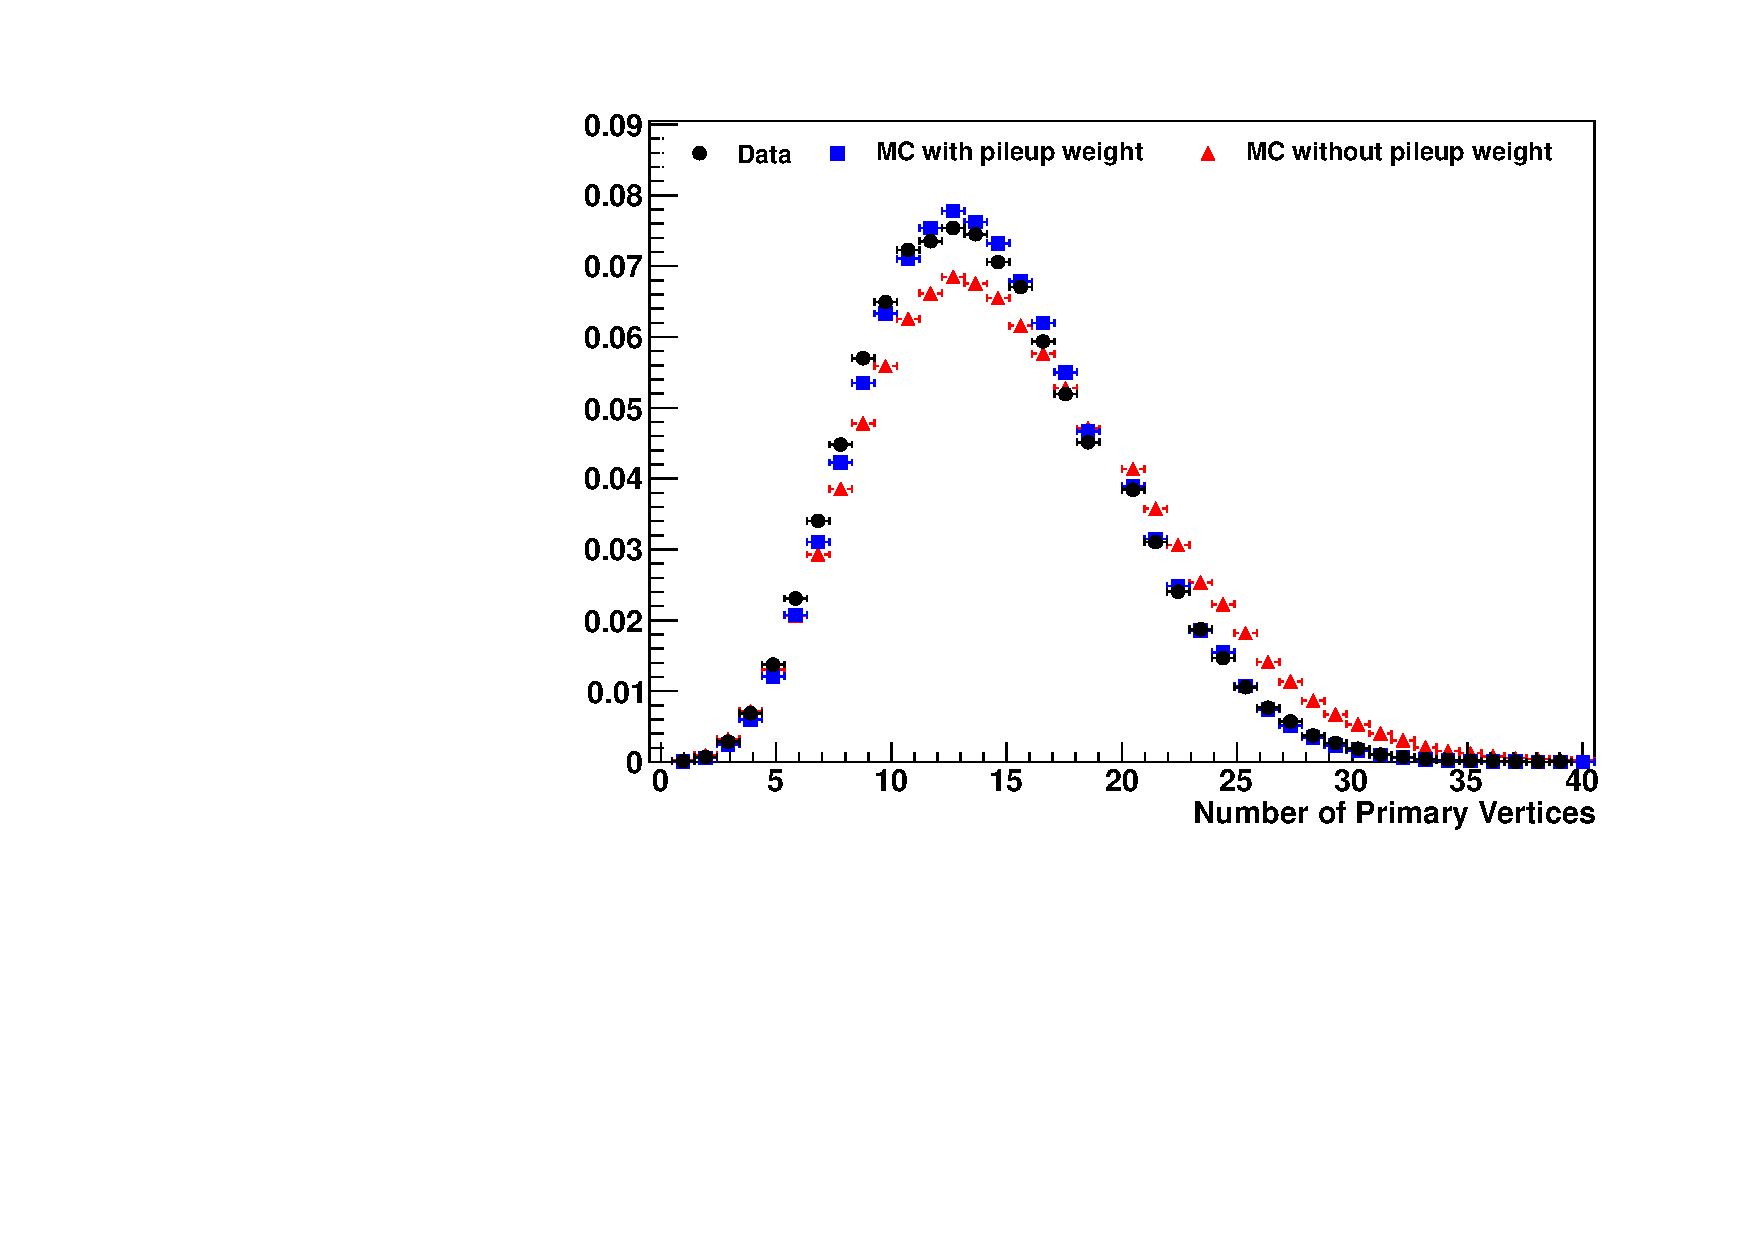
\includegraphics[width=0.5\textwidth]{Figures/Analysis_2_Diagrams/pileUpReWeighting_4Jincl2Tincl.pdf}
   \caption{Comparison of number of reconstructed vertices for data
     (black) and the sum of all background MC samples before (red) and after (blue) pileup
     reweighting.  After pileup reweighting, the MC matches the data well.}
   \label{fig:PUrewgt}
 \end{center}
\end{figure}


\subsection{Top $\pt$ Reweighting}
\label{top_pt_reweighting_overview}

\par It has been observed that the spectra of leptons and jets
produced from top quark decays have softer $\pt$ distribution than are
predicted by the Monte Carlo.  Investigations have show that the \PT
spectra of leptons and jets is softer than data and have traced this
expected to the top quark $\pt$ distribution
\cite{CMS-PAS-TOP-12-028, CMS-PAS-TOP-12-027}.  Measurements of the
differential cross section for top pair production as a function of
the top quark $\pt$, have allowed for the creation of correction
factors for this effect.  These predictions of the $\ttbar+$jets Monte
Carlo are also more consistent with calculations done at approximate
NNLO accuracy.  This correction factor replaces the additional pileup
reweighting factor based on the $H_{T}$ distribution, binned by number
of reconstructed vertices.  

\par The scale factor used to correct the Madgraph top quark $\pt$
distributions are shown in figure \ref{fig:topptsys}.  The associated
uncertainty is a band shown in green, and corresponds to no correction
factor for the down variation, and a doubling of the correction factor
for the up variation.  The scale factors are taken from a polynomial
of the form:

\begin{align*}
SF &= 1.18246 + 2.10061\times 10^{-6} \pt \left(\pt - 2 \times 463.312 \right)
\end{align*}

\noindent For $\pt > 463.312 \GeVc$, a constant scale factor of $0.732$ is used.


\begin{figure}[hbtp]
 \begin{center}
   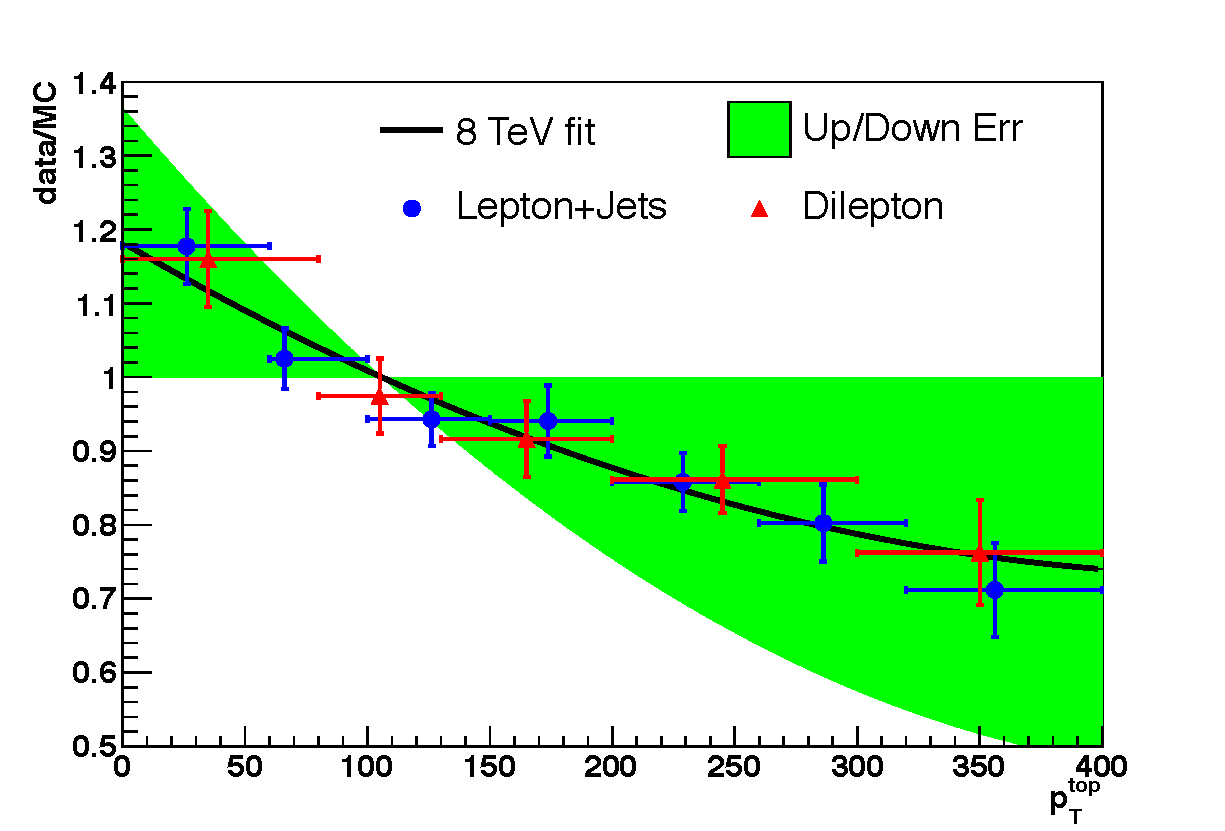
\includegraphics[width=0.7\textwidth]{Figures/Analysis_2_Diagrams/topptsys.pdf}
   \caption{The scale factors from top differential crosse section
     group, the fitting as well as the $\pm1\sigma$
     variations.}
   \label{fig:topptsys}
   \end{center}
\end{figure}


\par The top $\pt$ scale factor improves the agreement
between data and Monte Carlo. Figure \ref{fig:topPtBeforeAfter}
compares the leading jet $\pt$ distributions before and after
reweighting. Before the correction, the
leading jet $\pt$ ratio plot forms a line with a slope, which is
removed after the correction. 

\begin{figure}[hbtp]
 \begin{center}
   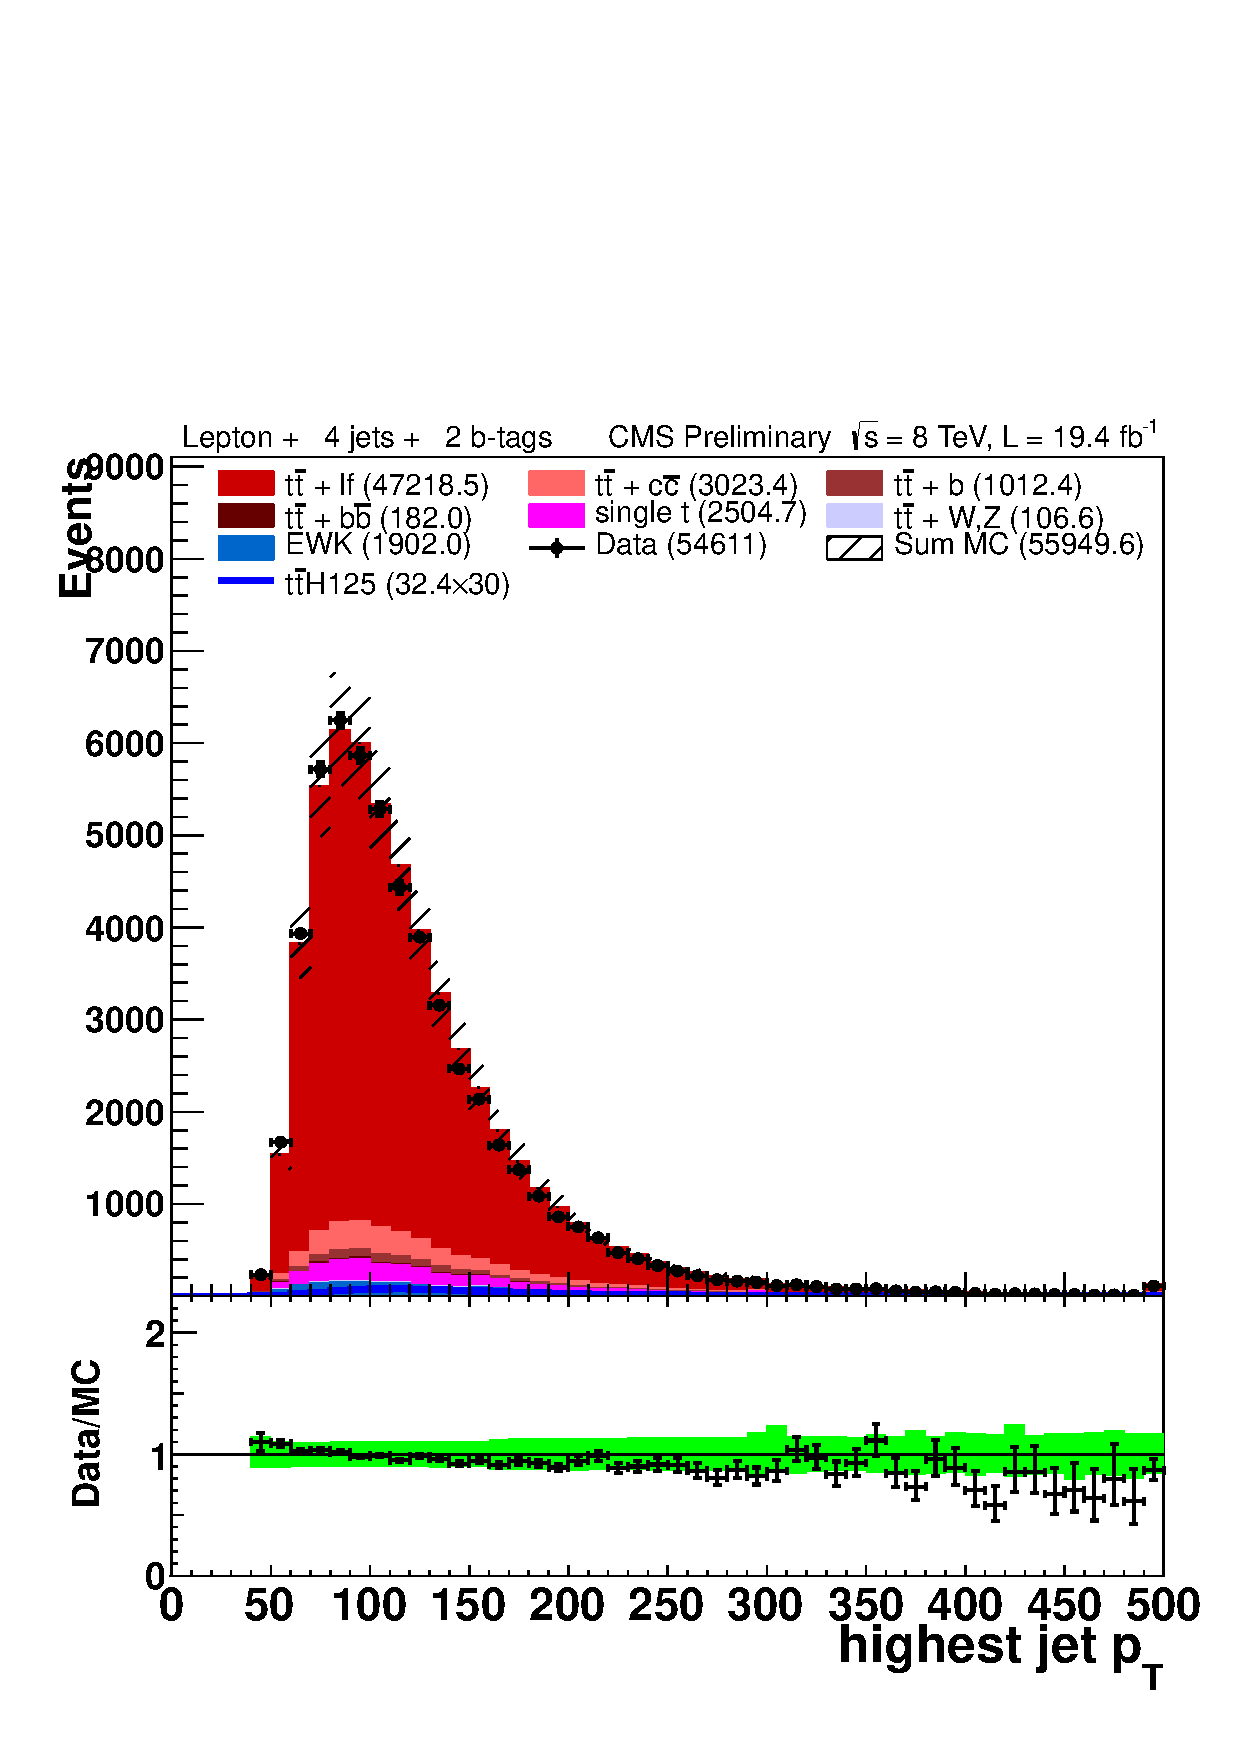
\includegraphics[width=0.45\textwidth]{Figures/Analysis_2_Diagrams/LJ_plots_lep/4j2t/lep_jet_pt_1_noTopPt_4j2t_cumulative_wRatio_lin.pdf}
   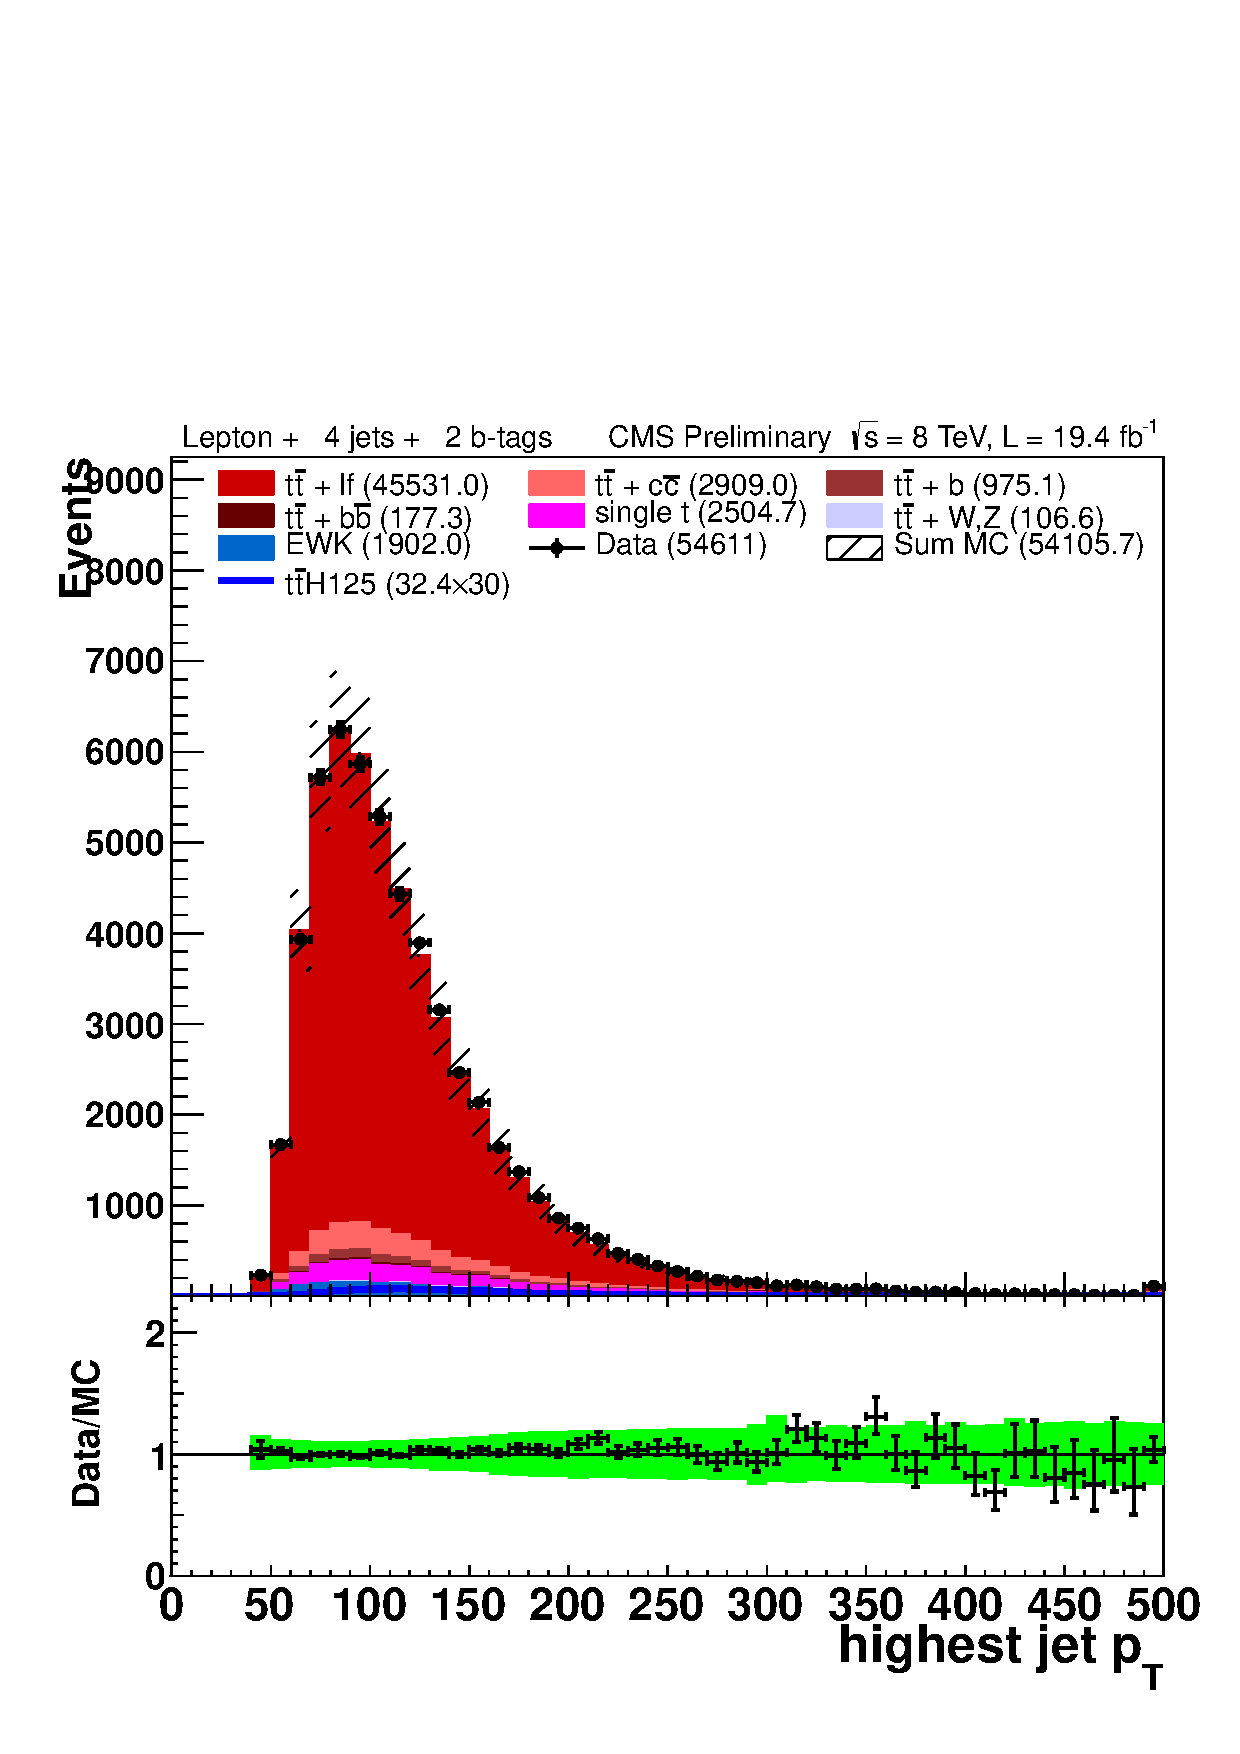
\includegraphics[width=0.45\textwidth]{Figures/Analysis_2_Diagrams/LJ_plots_lep/4j2t/lep_jet_pt_1_4j2t_cumulative_wRatio_lin.pdf}
   \caption{Leading jet $\pt$ distribution for 8 TeV lepton plus jet events with
   $\geq$4 jets and $\geq$2 tags. The left-hand plot shows the
   distribution before top $\pt$ reweighting. The right-hand plot shows the
   distribution after top $\pt$ reweighting. Note that the ratio in the right-hand
   plot is flatter than the left-hand plot.}
   \label{fig:topPtBeforeAfter}
   \end{center}
\end{figure}


\section{Event Selection}
\label{event_selection_II_overview}

\par This section defines the common physics objects and event
selection requirements.  Events are required to pass quality filters,
ensuring optimal operation of electronics and reconstruction, as
described in section \ref{event_cleaning_overview}.  The same lepton
selection is used that was employed in the previous analysis, with
events being selected by triggers described in section
\ref{trigger_II_overview}.  Leptons are classified into two
categories, tight and loose, defined for muons in section
\ref{muon_selection_overview} and for electrons in
\ref{electron_selection_overview}.  For this analysis, exactly one
tight muon or exactly one tight electron is required and events with 
any additional loose leptons are rejected.  Lepton reconstruction
efficiency scale factors are discussed
in \ref{trigger_efficiency_overview}.  The selection for jets is
also the same, with the same procedure for correcting the energy as in
section \ref{jet_selection_overview}.  The only significant change to
the event selection comes from the $b$-tag scale factors used to
calibrate the differences between efficiency in data and simulation
for the CSV algorithm.  

\subsection{$b$-tag discriminant reweighting}
\label{b_tag_reweighting_overveiw}

\par As described in section \ref{btag_overview}, the algorithm used
to tag jets as coming from a $b$-quark, is the Combined Secondary
Vertex (CSV) algorithm.  Differences have been observed in the
measured efficiency for $b$-tagging jets between data and
simulation~\cite{CMS-PAS-BTV-11-004}.  To account for these efficiency
differences, a scale factor to correct the MC $b$-tagging
efficiency. Moreover, we found that the CSV distribution 
of MC doesn't match that of data, there making it necessary to correct
the shape of the discriminant distribution as well.  

\par A $b$-tag CSV reweighting method has been developed to address
not only the difference in efficiency, but the difference in the shape
of the discriminant distribution as well \cite{CMS-AN-2013-130}.  
The method is based on a "tag and probe'' approach.   Events with two
leptons, and exactly two jets are initially selected.  One jet is
required to pass a "tight'' working point, characterized by a CSV
value with $\sim90\%$ efficiency and $\le1\%$ mistag rate.  Then, the
other jet is required to pass the analysis working point to assess the
efficiency there.  The results are binned by $p_{T}$, $\eta$, jet
flavor and CSV value.  

\par For MC the truth is available to assess the efficiency.  For
data, the full 8~TeV DoubleMu, DoubleElectron and MuEG datasets taken
in 2012 are used. The scale factors for heavy flavor jets were derived in the
dilepton channel, using a $t\bar{t}$ enriched control sample dominated
by events which have two $b$ flavor jets from the top pair decay.  The
scale factors for light flavor jets in the dilepton channel, using a
control sample dominated by $Z$+jets events where there are two light
flavor jets. The scale factors for light flavor jets will account for
the mis-tag efficiency discrepancy between data and MC. For events
with one jet passing the tag requirements, the CSV
distribution for the probe jet in given $p_{t}$ and $\eta$ 
bins. The total MC yields are normalized to the data yields. In order to
account for heavy or light flavor contamination, the MC is divided into
samples of heavy flavor and light flavor components and then
non-relevant part from data is subtracted. The scale factor is then
given by the ratio of subtracted data CSV distribution and the relevant MC
CSV distribution, as shown below:

\begin{equation}
SF(CSV, p_{t}, \eta) = \frac{Data - MC_{A}}{MC_{B}} 
\end{equation}

\noindent where A, B = heavy flavor component or light flavor component.

\par Unlike the last analysis, where scale factors where applied to
adjust the value of the CSV distribution, correction factor for this
analysis is an event-by-event weight.  If the jet is a $b$ flavor jet,
a heavy flavor scale factor is assigned to it; if it is a $c$ flavor
jet, a flat scale factor of 1.0 is applied, with the same uncertainty
as a $b$ flavor jet would receive; otherwise, if it is a
light flavor jet, a light flavor scale factor is assigned.  The total
scale factor for the event is the product of all the scale factors of
the jets: 

\begin{equation}
SF_{total} = \prod_{i}^{N_{\mathrm{jets}}} SF_{jet_{i}} = SF_{jet_{1}} \cdot SF_{jet_{2}} \cdot ...
\end{equation}


\subsection{Lepton + Jets Selection}
\label{LJ_selection_II_overview}

\par As with the previous analysis, the final selection requires
events have exactly one tight lepton ($e$ or $\mu$), and at least four
jets. Events with any additional loose or tight leptons are vetoed so
this analysis can later be combined with a diLepton final state,
without double counting events. Additionally, each event must have at
least three jets with $p_{T} > 40$ GeV/c. 

\par As before, events are further categorized by the reconstructed jet, and
$b$-tagged jet multiplicities:

\begin{itemize}
  \item $\ge$6 jets,  $==$2 $b$-tags: At least 6 jets, 2 of which are $b$-tagged 
  \item $==$4 jets, $==$3 $b$-tags: Exactly 4 jets, 3 of which are $b$-tagged 
  \item $==$5 jets, $==$3 $b$-tags: Exactly 5 jets, 3 of which are $b$-tagged 
  \item $\ge$6 jets, $==$3 $b$-tags: At least 6 jets, 3 of which are $b$-tagged 
  \item $==$4 jets, $==$4 $b$-tags: Exactly 4 jets, 4 of which are $b$-tagged 
  \item $==$5 jets, $==$4 $b$-tags: Exactly 5 jets, 4 of which are $b$-tagged 
  \item $\ge$6 jets, $\ge$4 $b$-tags: At least 6 jets, with at least 4 of which are $b$-tagged 
\end{itemize}


\par Table~\ref{tab:dataMC_LJeventyield} gives the event yield for MC
backgrounds, both the total and each contribution, the expected event
yield for signal \(t\bar{t}H\) (\(m_{H}\) = 125 GeV/c$^2$), and the
data observed in each category. Figure~\ref{fig:LJ_numJets_numTags}
shows the data/MC comparison for the number of jets and the number of
tagged jets distributions for events with one lepton (\(e\) or
\(\mu\)), \(\ge\) 4 jets and \(\ge\) 2 b-tags, it also includes a plot
showing the event yields for data and each MC background in each
category. 

\begin{figure}[hbtp]
\begin{center}
 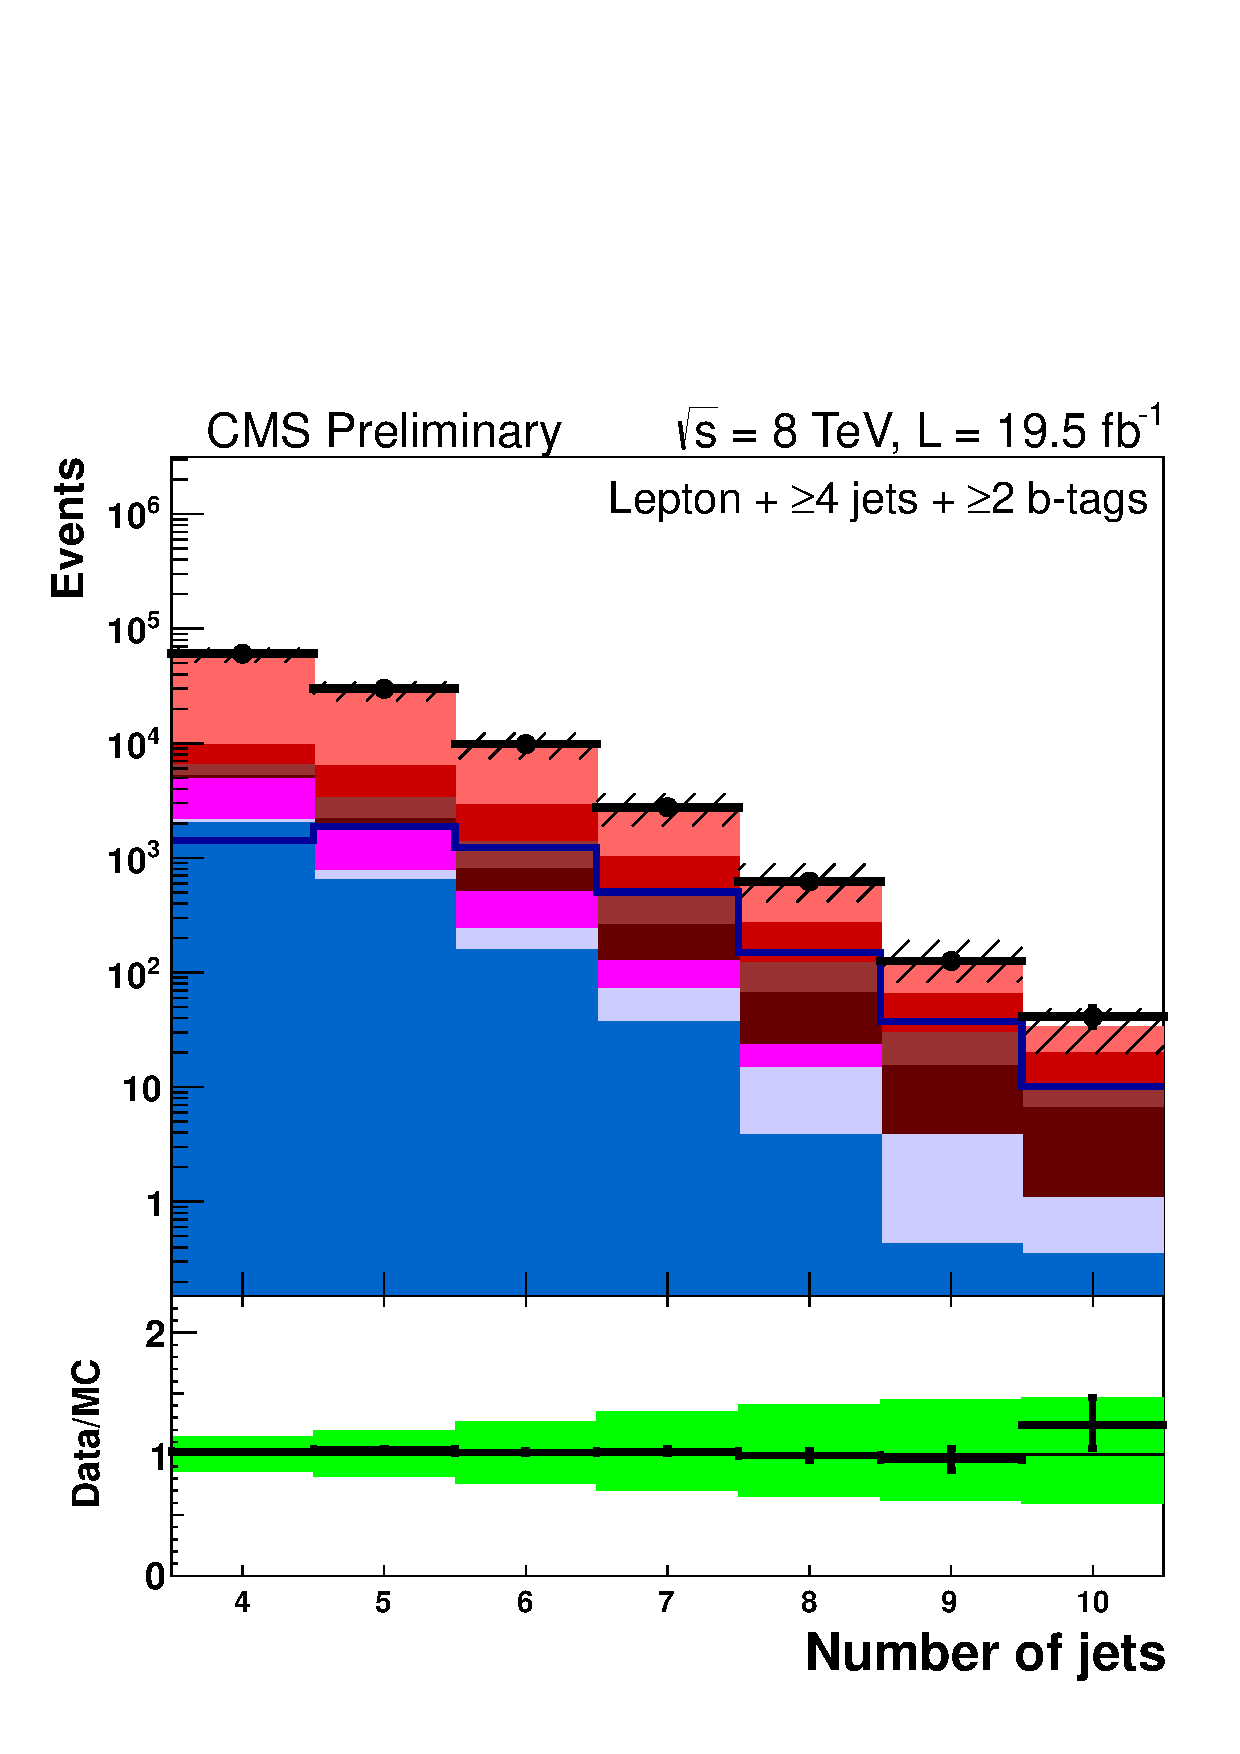
\includegraphics[width=0.45\textwidth]{Figures/Analysis_2_Diagrams/LJ_plots_lep/lep_numJet_cumulative_wRatio_noLegend_log.pdf}
 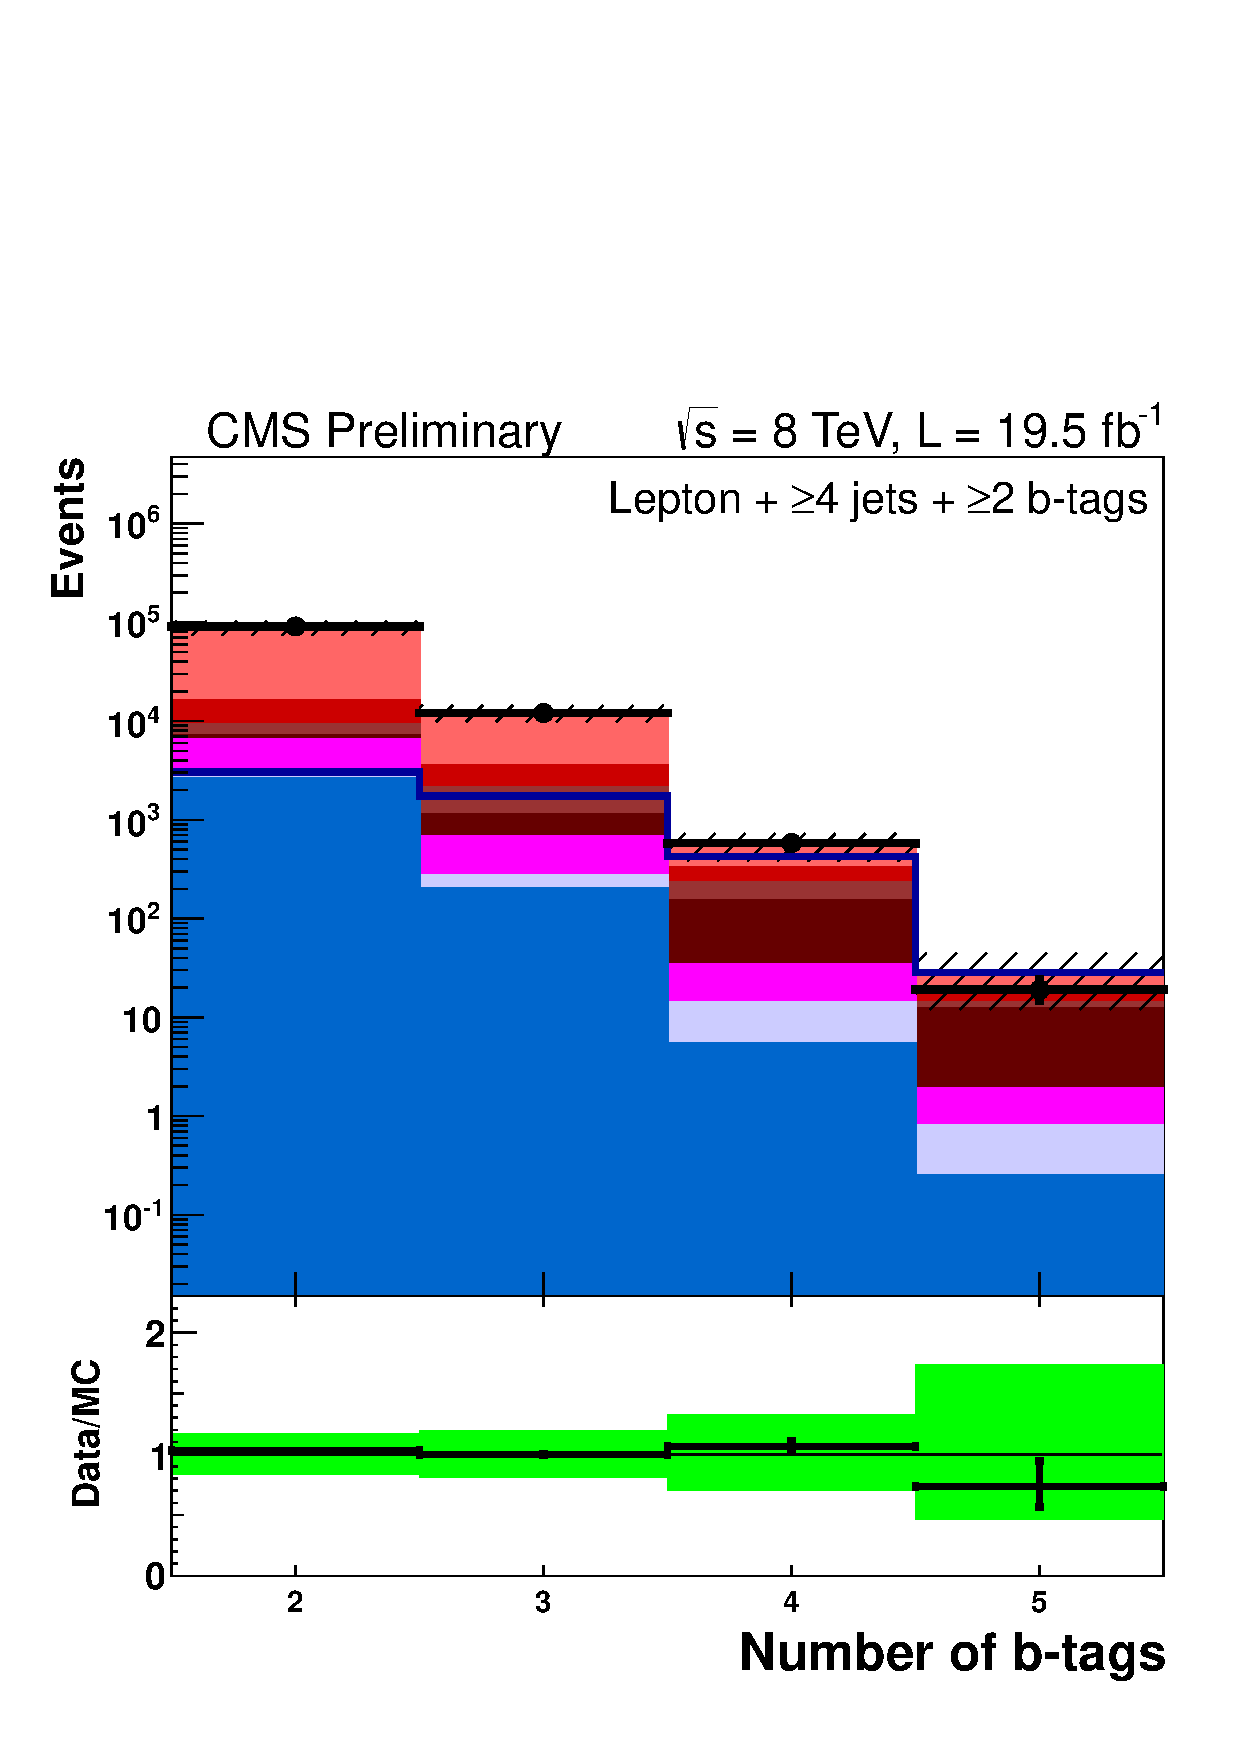
\includegraphics[width=0.45\textwidth]{Figures/Analysis_2_Diagrams/LJ_plots_lep/lep_numTag_cumulative_wRatio_noLegend_log.pdf}
   \caption{Comparison of yields for the different categories (top), number of jets (bottom left), and number of tagged jets (bottom right) in data and Monte Carlo for events
    with one lepton $\mu$ or $e$, $\ge$ 4 jets and $\ge$ 2 tags.  }
   \label{fig:LJ_numJets_numTags}
 \end{center}
\end{figure}


\begin{table}[!ht]
\begin{center}
  \noindent
  \small
    \begin{tabular}{|l|c|c|c|c|c|c|c|} \hline
& $\geq$6 jets & 4 jets & 5 jets & $\geq$6 jets & 4 jets & 5 jets & $\geq$6 jets \\
& 2 tags & 3 tags & 3 tags & 3 tags & 4 tags & $\geq$4 tags & $\geq$4 tags \\ \hline \hline
$t\bar{t}H(125)$ & 33.4 $\pm$ 8.1 & 14.0 $\pm$ 3.0 & 21.1 $\pm$ 4.5 & 23.1 $\pm$ 5.5 & 1.8 $\pm$ 0.5 & 5.2 $\pm$ 1.4 & 8.3 $\pm$ 2.3 \\
 \hline
$t\bar{t}+$lf & 7650 $\pm$ 2000 & 4710 $\pm$ 820 & 2610 $\pm$ 530 & 1260 $\pm$ 340 & 74 $\pm$ 30 & 79 $\pm$ 34 & 71 $\pm$ 36 \\
$t\bar{t}+b$ & 530 $\pm$ 300 & 350 $\pm$ 190 & 360 $\pm$ 200 & 280 $\pm$ 160 & 21 $\pm$ 12 & 29 $\pm$ 17 & 33 $\pm$ 20 \\
$t\bar{t}+b\bar{b}$ & 220 $\pm$ 120 & 99 $\pm$ 52 & 158 $\pm$ 85 & 200 $\pm$ 110 & 13.1 $\pm$ 7.3 & 38 $\pm$ 21 & 78 $\pm$ 47 \\
$t\bar{t}+c\bar{c}$ & 1710 $\pm$ 1110 & 440 $\pm$ 230 & 520 $\pm$ 290 & 470 $\pm$ 280 & 19 $\pm$ 11 & 32 $\pm$ 18 & 52 $\pm$ 31 \\
$t\bar{t}V$ & 99 $\pm$ 27 & 16.2 $\pm$ 3.8 & 23.9 $\pm$ 5.7 & 28.8 $\pm$ 7.4 & 1.1 $\pm$ 0.4 & 2.5 $\pm$ 0.7 & 5.8 $\pm$ 1.8 \\
Single $t$ & 264 $\pm$ 54 & 235 $\pm$ 41 & 116 $\pm$ 22 & 55 $\pm$ 14 & 3.4 $\pm$ 1.6 & 10.3 $\pm$ 5.3 & 7.3 $\pm$ 3.1 \\
$V+$jets & 160 $\pm$ 110 & 122 $\pm$ 95 & 44 $\pm$ 38 & 29 $\pm$ 27 & 2.1 $\pm$ 2.4 & 1.9 $\pm$ 1.7 & 1.2 $\pm$ 1.3 \\
Diboson & 5.9 $\pm$ 1.6 & 6.3 $\pm$ 1.4 & 2.4 $\pm$ 0.7 & 1.0 $\pm$ 0.4 & 0.3 $\pm$ 0.2 & 0.1 $\pm$ 0.1 & 0.2 $\pm$ 0.1 \\
 \hline
Total bkg & 10630 $\pm$ 2790 & 5970 $\pm$ 1060 & 3830 $\pm$ 790 & 2310 $\pm$ 620 & 133 $\pm$ 44 & 193 $\pm$ 62 & 249 $\pm$ 90 \\
 \hline
Data & 10724 & 5667 & 3983 & 2426 & 122 & 219 & 260 \\
\hline
\end{tabular}
    \caption{Observed data event yields, expected event yields in 19.5 fb$^{-1}$ for signal and backgrounds in the lepton+jets channel.}
    \label{tab:dataMC_LJeventyield}
\end{center}
\end{table}

\section{Multivariate Analysis}
\label{mva_II_overview}

\par The MVA technique used to analyze the full 8 TeV dataset is a
Boosted Decision Tree (BDT).  Each jet/tag category is trained with
half of the simulated \ttH events for signal, and half of the
simulated \ttjets events as background.  The top 10 variables, ranked
with the separation figure of merit given in equation
\ref{eq:separation}, are used as input variables.  The BDT
distribution of the discriminant is then used for signal extraction
and limit setting. 


\subsection{Boosted Decision Tree Overview}
\label{bdt_overview}

\par A Boosted Decision Tree (BDT) is a code structure that makes a
sequence of binary decisions to classify events as either signal-like
or background-like \cite{Hocker:2007ht}.  For this analysis, the BDT
uses 10 input variables for each jet/tag category.  The BDT looks at
the distribution of events for signal and background, with 40 bins
with a maximum and minimum value determined by the the largest and
smallest values respectively for either the signal or the background.
Out of these 10 variables, the BDT selects the variable which
maximizes the Ginni Index, which is given by the equation:

\begin{equation}\label{eq:gini_index}
Gini Index = p\times(1 - p)
\end{equation}

\noindent where the purity, $p=s/b$, is the ratio of the integral
number of signal, $s$, events and background, $b$, events above or
below the cut value chosen by the BDT.  This effectively tries to find
a cut on a variable that maximizes the amount signal in sample
afterwards, creating a background-like set of events, and a
signal-like set of events.  After the first cut is chosen, the
distributions for each of the variables above and below the cut value
are are re-examined.  A second cut on a variable, at a point that
maximizes the Ginni Index is found, for each of the signal and
background-like regions formed by the first cut.  This process
continues for a user-defined number of cuts.  Since the input events
are known to be singal-like or background-like, the purity of the
final region that an event is classified as is used as the output for
this set of decisions, known as a decision tree.  Figure
\ref{fig:decision_tree} shows a diagram of the general process.

\begin{figure}[hbtp]
\begin{center}
 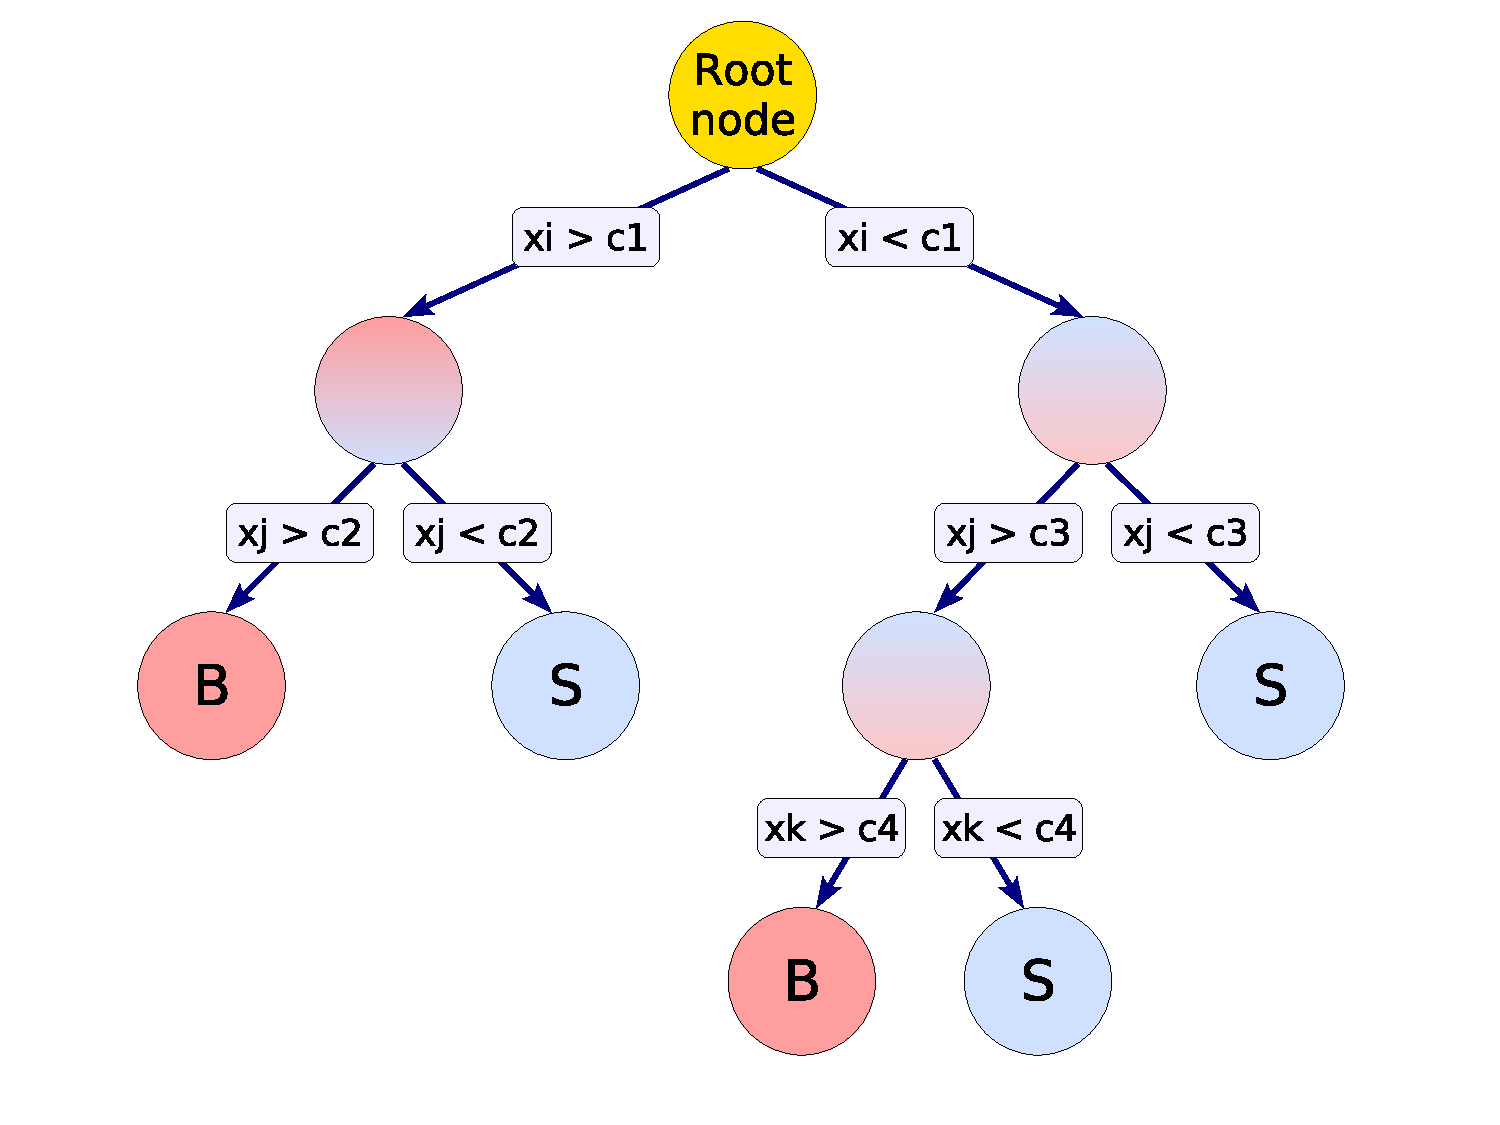
\includegraphics[width=0.45\textwidth]{Figures/Analysis_2_Diagrams/BDT_example.pdf}
   \caption{Example of a decision tree, which chooses a set of
     variables to cut on, in order to produce a region of events with
     high signal purity }
   \label{fig:decision_tree}
 \end{center}
\end{figure}

\noindent  The BDT in this analysis uses 5 cuts for a single tree.
The reason for using a small number, is that the BDT employs a process
known as "boosting'' to enhance its discriminating power.  

\par Boosting is the process of using multiple, or a forest, of
individual decision trees to cast a majority vote for the decision to
classify the event as signal-like or background-like
\cite{Hocker:2007ht}.  Events from the training sample, which were
misclassified, are given a larger weight, making their contribution to
the distributions of the input variable more prominent, making it more
likely for the next decision tree to classify the event correctly.
The final discriminant, $F(\hat{x},P)$, of the forest of decision
trees is given by: 

\begin{equation}\label{eq:bdt_discriminant}
F(\hat{x}, P) = \sum_{m=0}^{M}\beta_{m}f(x;a_{m});
~~~~P\in(\beta_{m};a_{m})_{0}^{M}
\end{equation}

\noindent where $P$ is the set of parameter, whose values are
optimized to create an optimized classification decision.  For $M$
trees in the forest, $\beta_{m}$ is the weight for the output of a
single decision tree, $f(x;a_{m})$, which is the purity, $s/b$ of the
final region of the tree an individual event is classified into.  The
set of input variables for a single decision tree, $m$, is denoted by
$a_{m}$.   

\par This analysis uses the "Gradient'' method of boosting
\cite{Hocker:2007ht}.  After the first tree is has been built, the
"loss function'', $L(F,y)$, is calculated with the function:

\begin{equation}\label{eq:bdt_loss_function}
L(F,y) = ln\left( 1+ e^{-2F(\hat{x})y}\right)
\end{equation}

\noindent where $y$ is the true value of the classification of the
event (1 for signal, 0 for background).  This function has a minimum
value when all of the events have been classified correctly.  The loss
function is then minimized by varying the set of parameters,
$P\in(\beta_{m};a_{m})_{0}^{M}$, using the steepest-descent method.  A
random selection of events are reweighted, and the loss-function is
re-calculated.  The error rate of classifying events for the previous
tree is used to calculate the new weight, $\alpha$, of events for the
next tree: 

\begin{equation}\label{bdt_event_reweight}
\alpha = \frac{1-err}{err}
\end{equation}

\noindent where $err$ is the error rate.  After events are
re-weighted, a new decision tree is created and the process is
repeated, iteratively minimizing the loss function until a desired set
of decision trees are created.  This analysis uses a forest of 100
decision trees to separate the \ttH signal from the \ttjets
background.  

\par  Overtraining was checked in a similar procedure that was used in
the last analysis.  Half the events for the signal and background
samples are used to train the BDT, the other half are used to test
it.  The response to the BDT is calculated for both the testing and
training sample, and the Kolomogrov-Smirnoff statistic is used as a
figure of merit to judge the compatibility of the two samples.  As
seen in figure \ref{fig:bdt_testTrain}, there are no significant
deviations between  the testing and training samples, implying that no
overtraining has occurred.  

\begin{figure}[hbtp]
 \begin{center}
   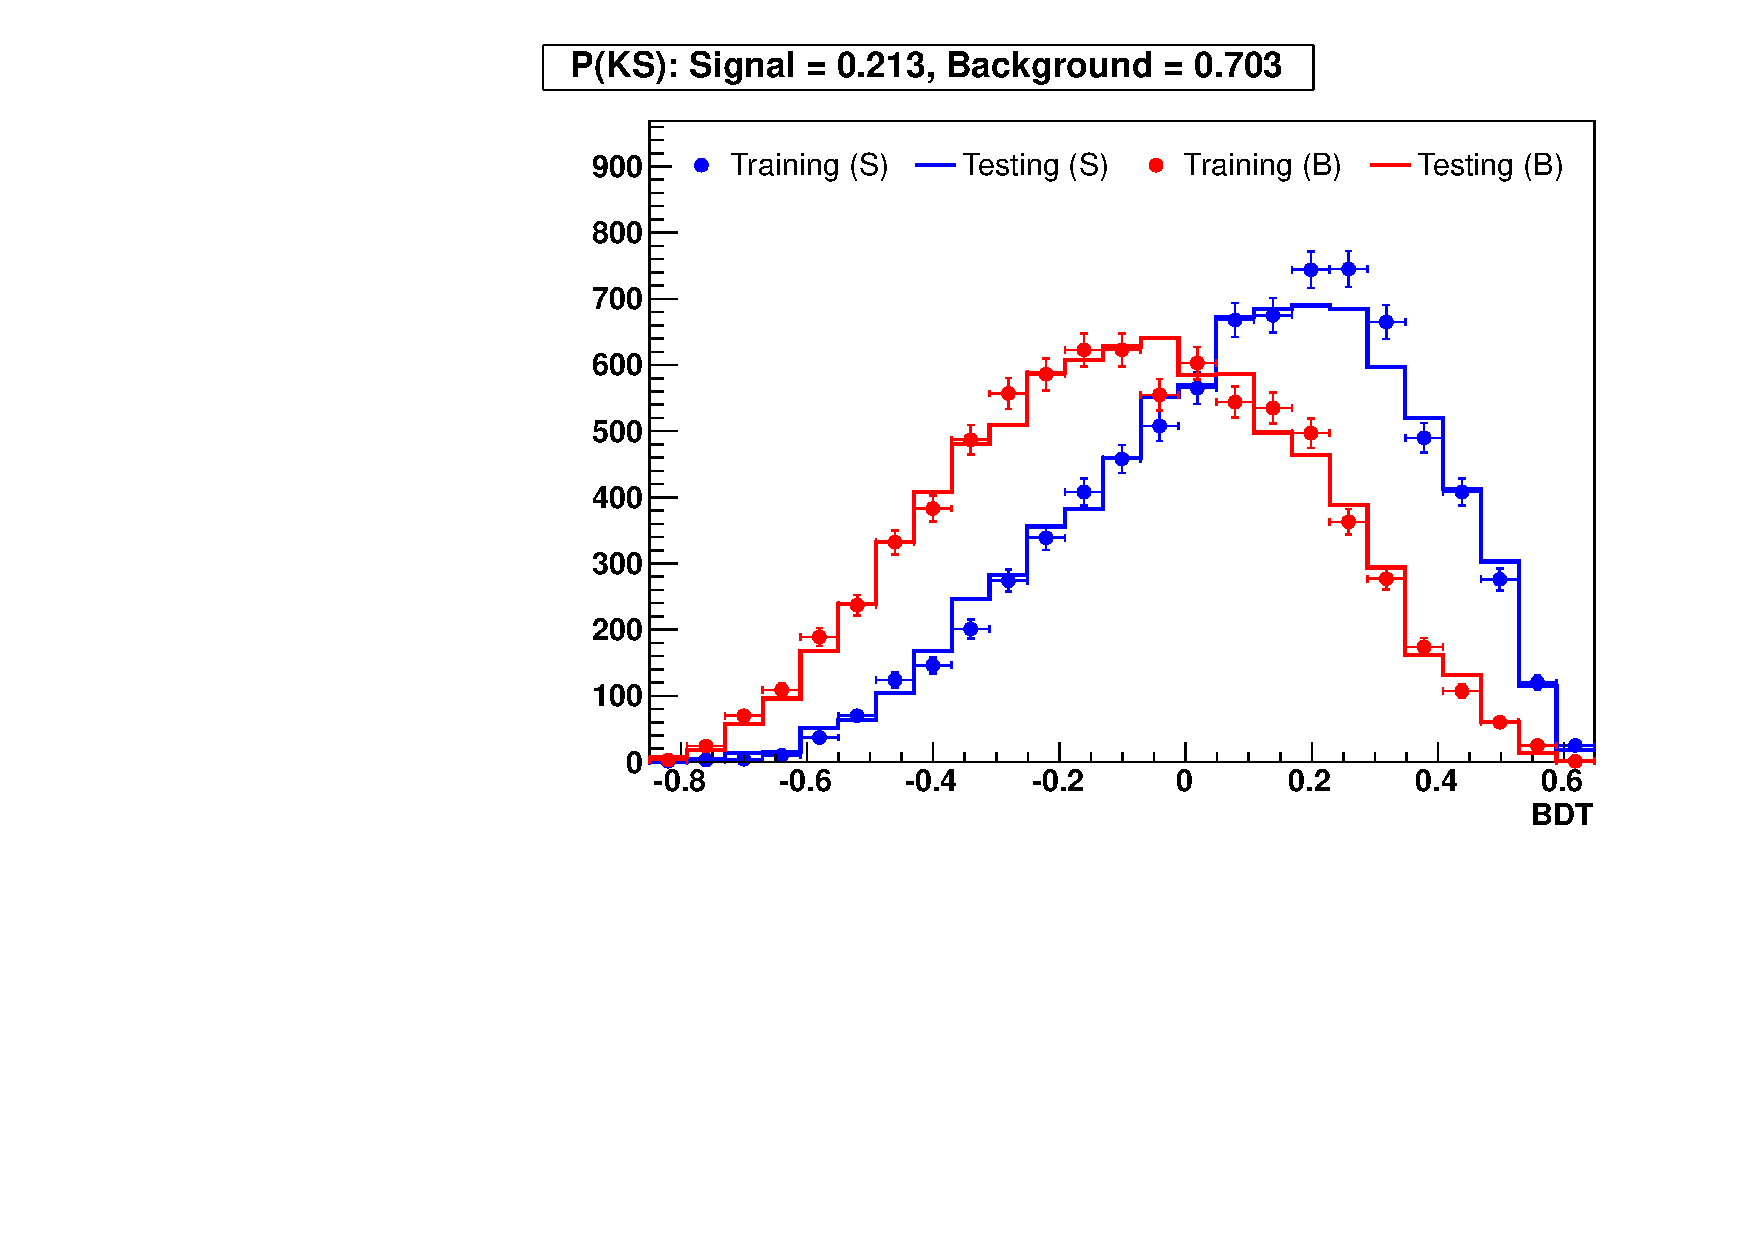
\includegraphics[width=0.45\textwidth]{Figures/Analysis_2_Diagrams/LJ_plots_lep/training/BDT_training_623.pdf}
   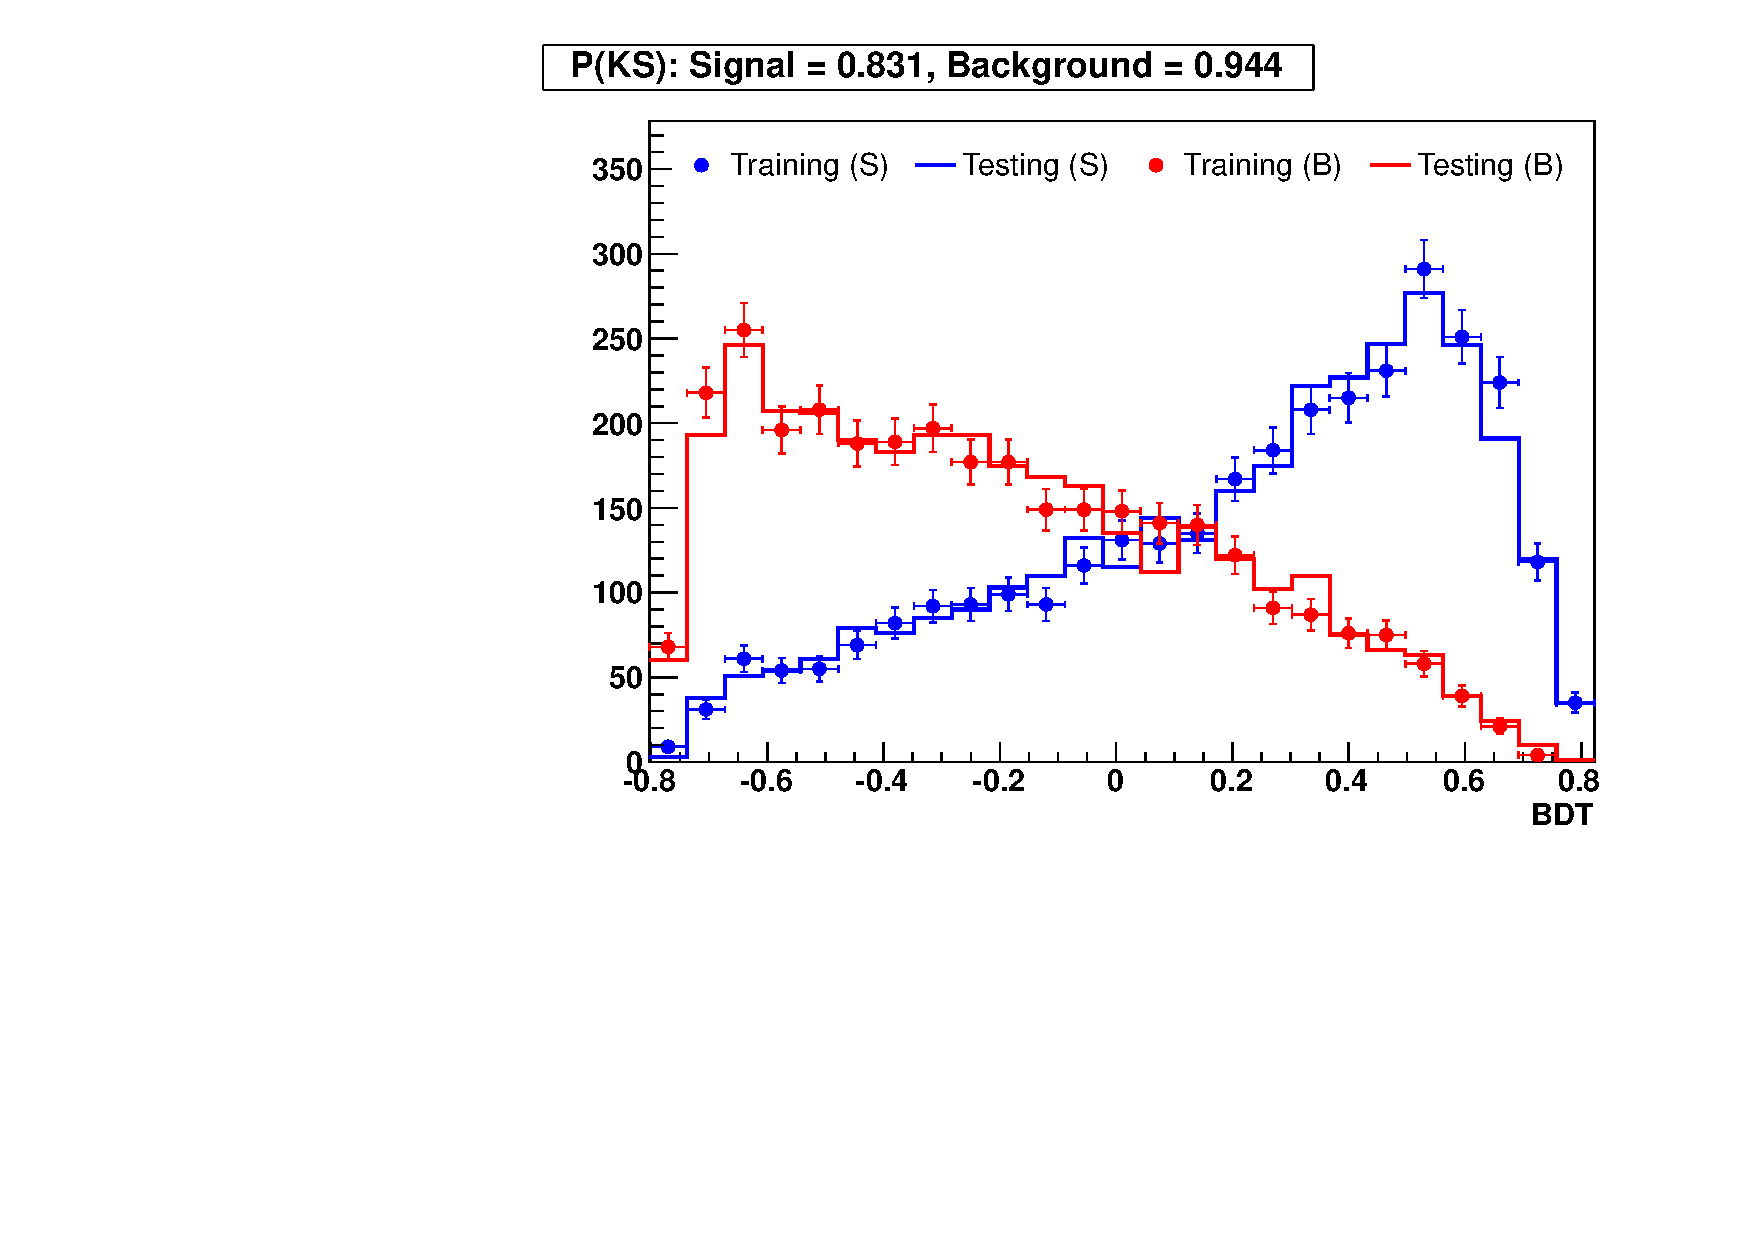
\includegraphics[width=0.45\textwidth]{Figures/Analysis_2_Diagrams/LJ_plots_lep/training/BDT_training_433.pdf}
   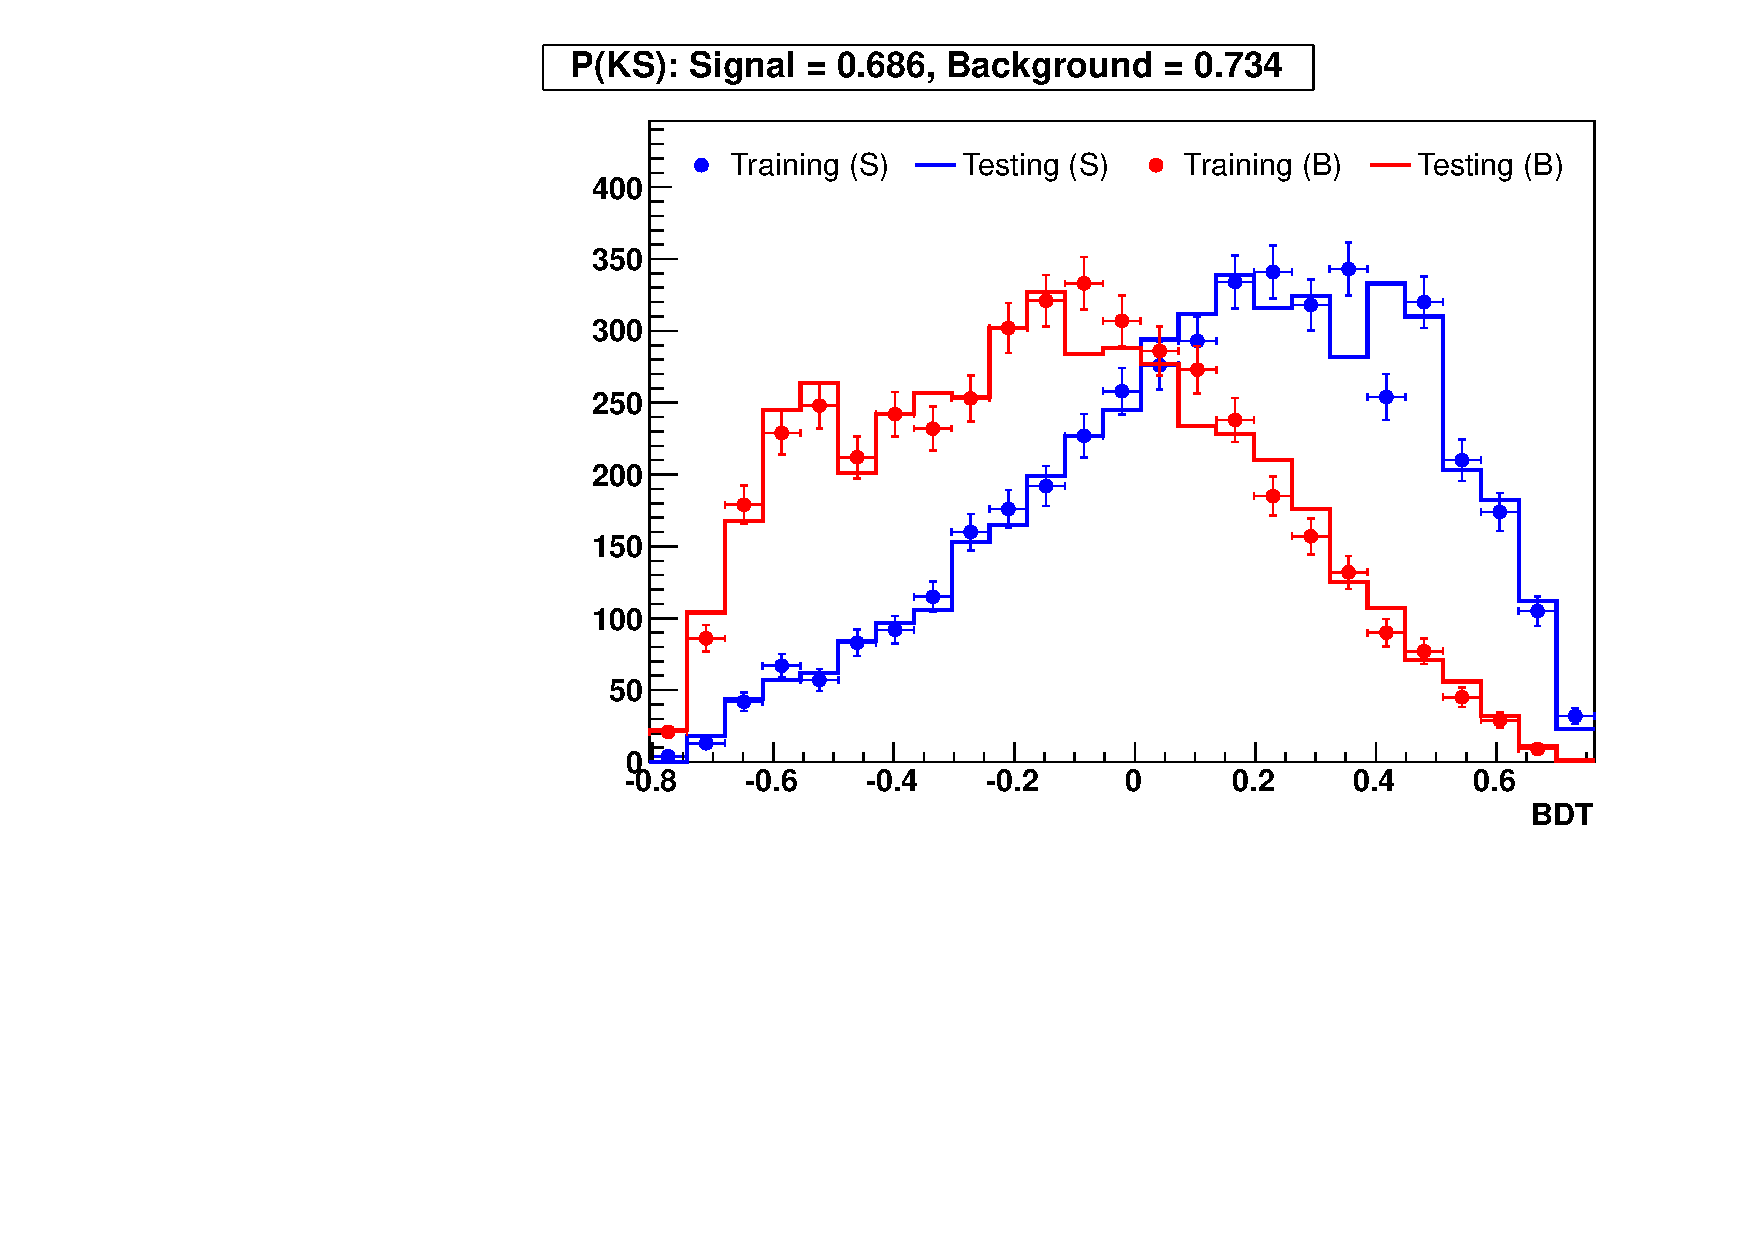
\includegraphics[width=0.45\textwidth]{Figures/Analysis_2_Diagrams/LJ_plots_lep/training/BDT_training_533.pdf}
   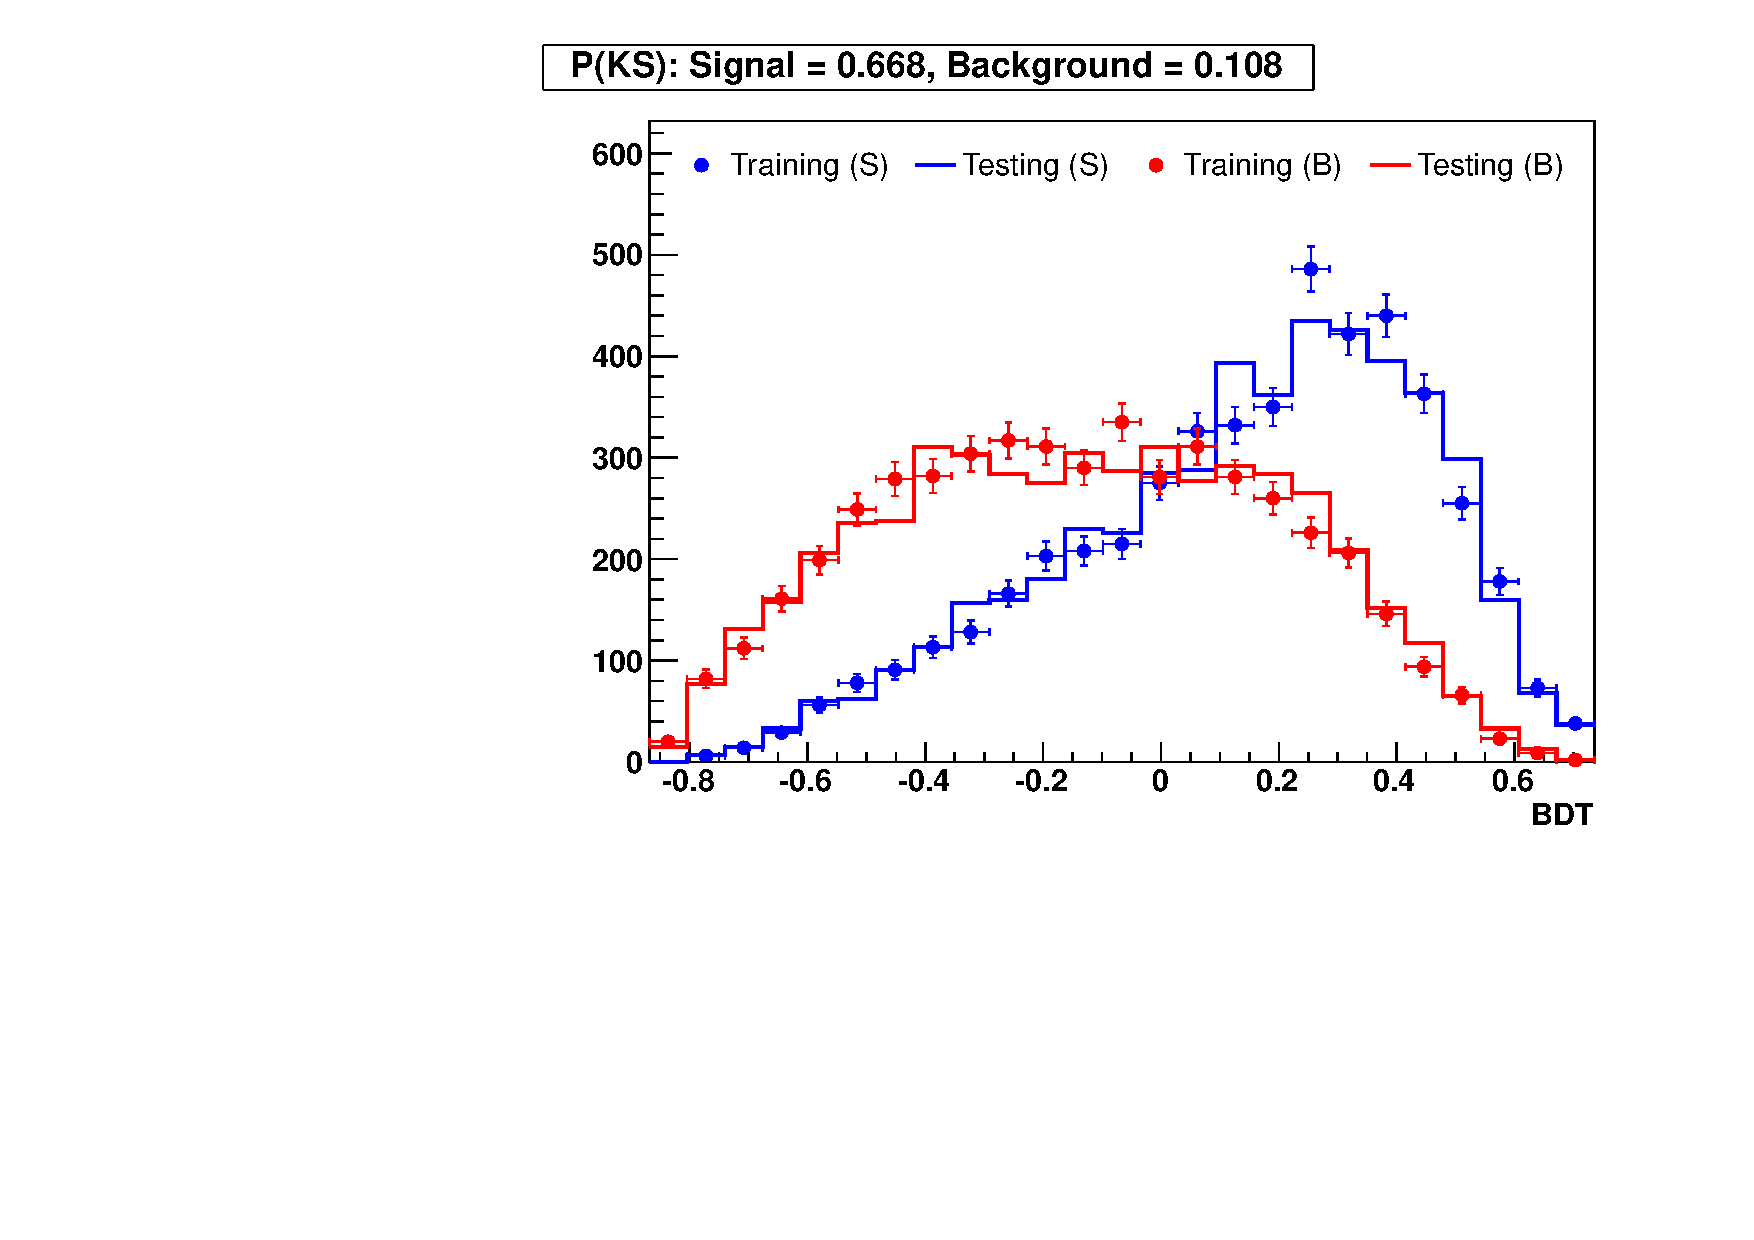
\includegraphics[width=0.45\textwidth]{Figures/Analysis_2_Diagrams/LJ_plots_lep/training/BDT_training_633.pdf}
   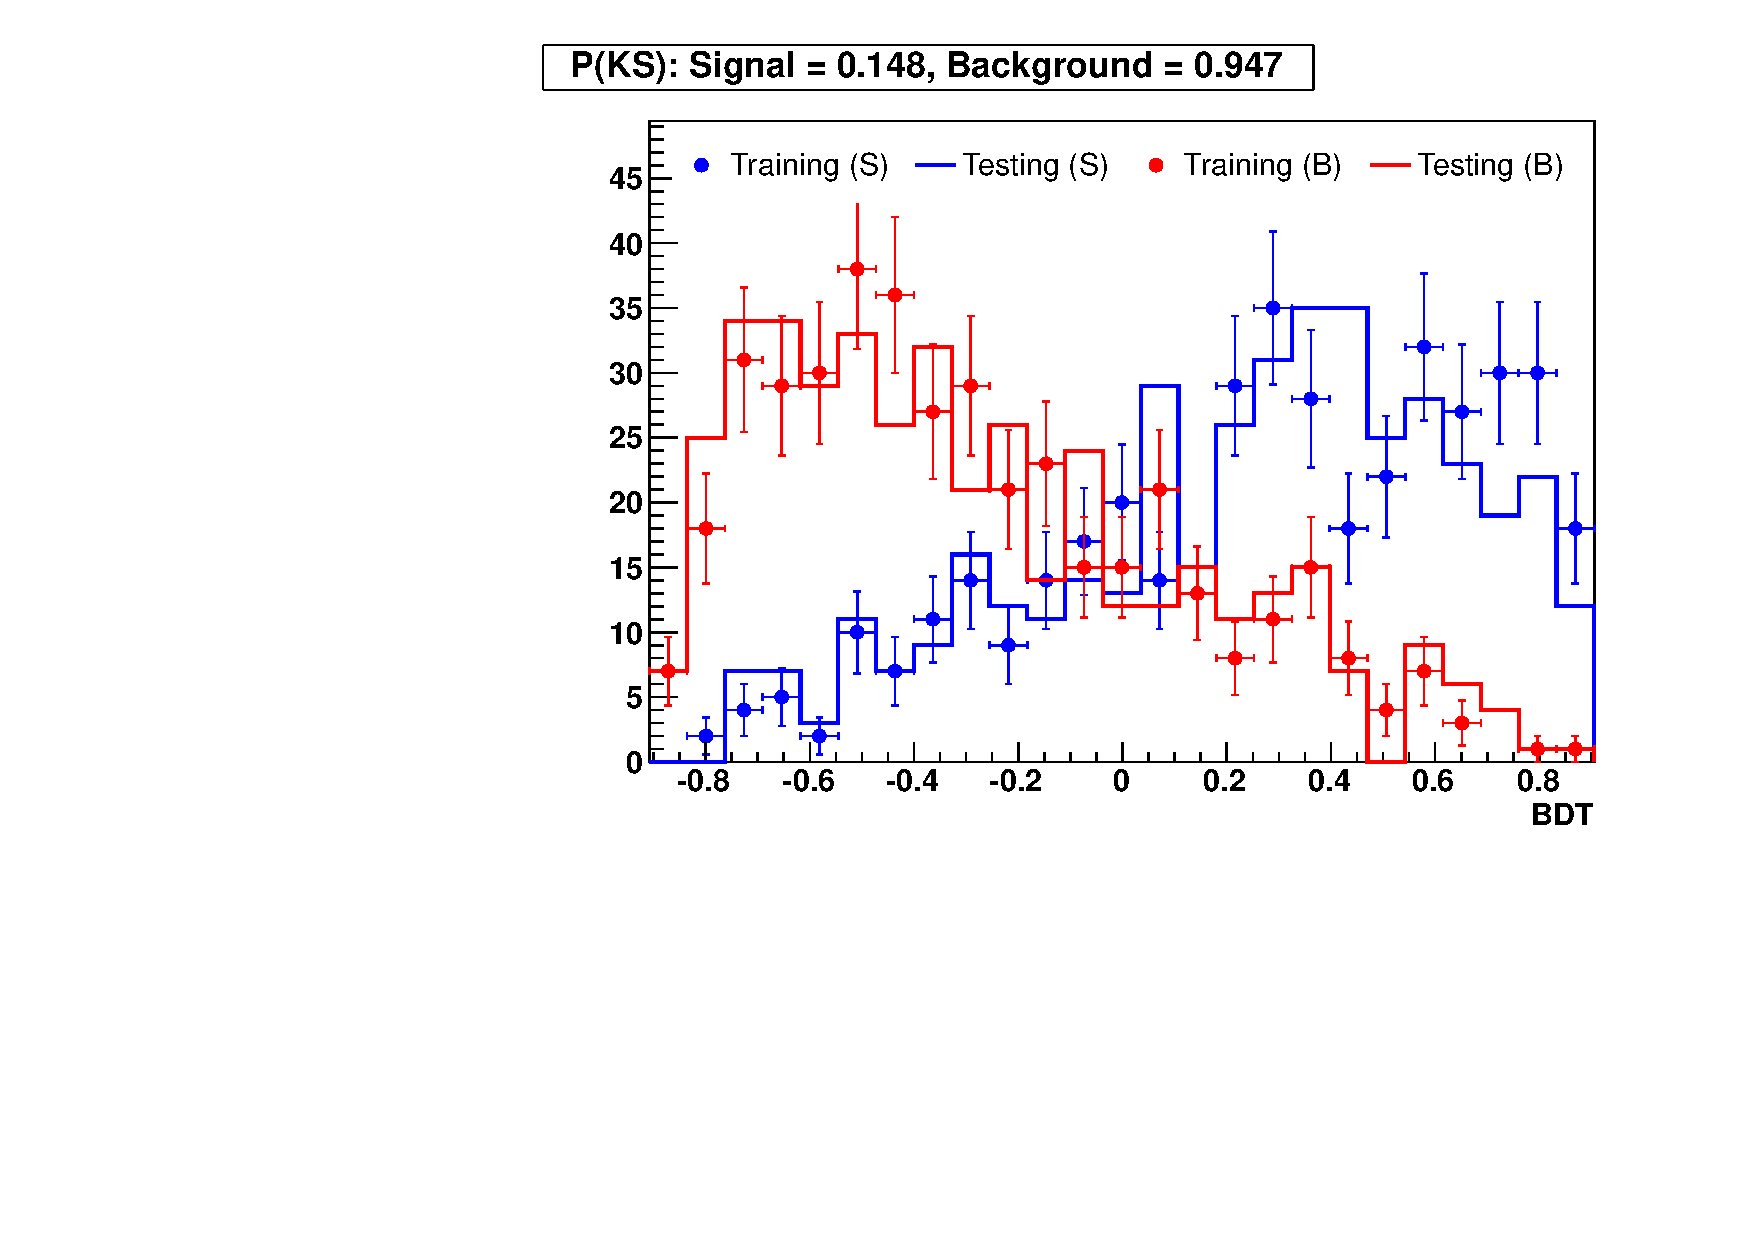
\includegraphics[width=0.45\textwidth]{Figures/Analysis_2_Diagrams/LJ_plots_lep/training/BDT_training_443.pdf}
   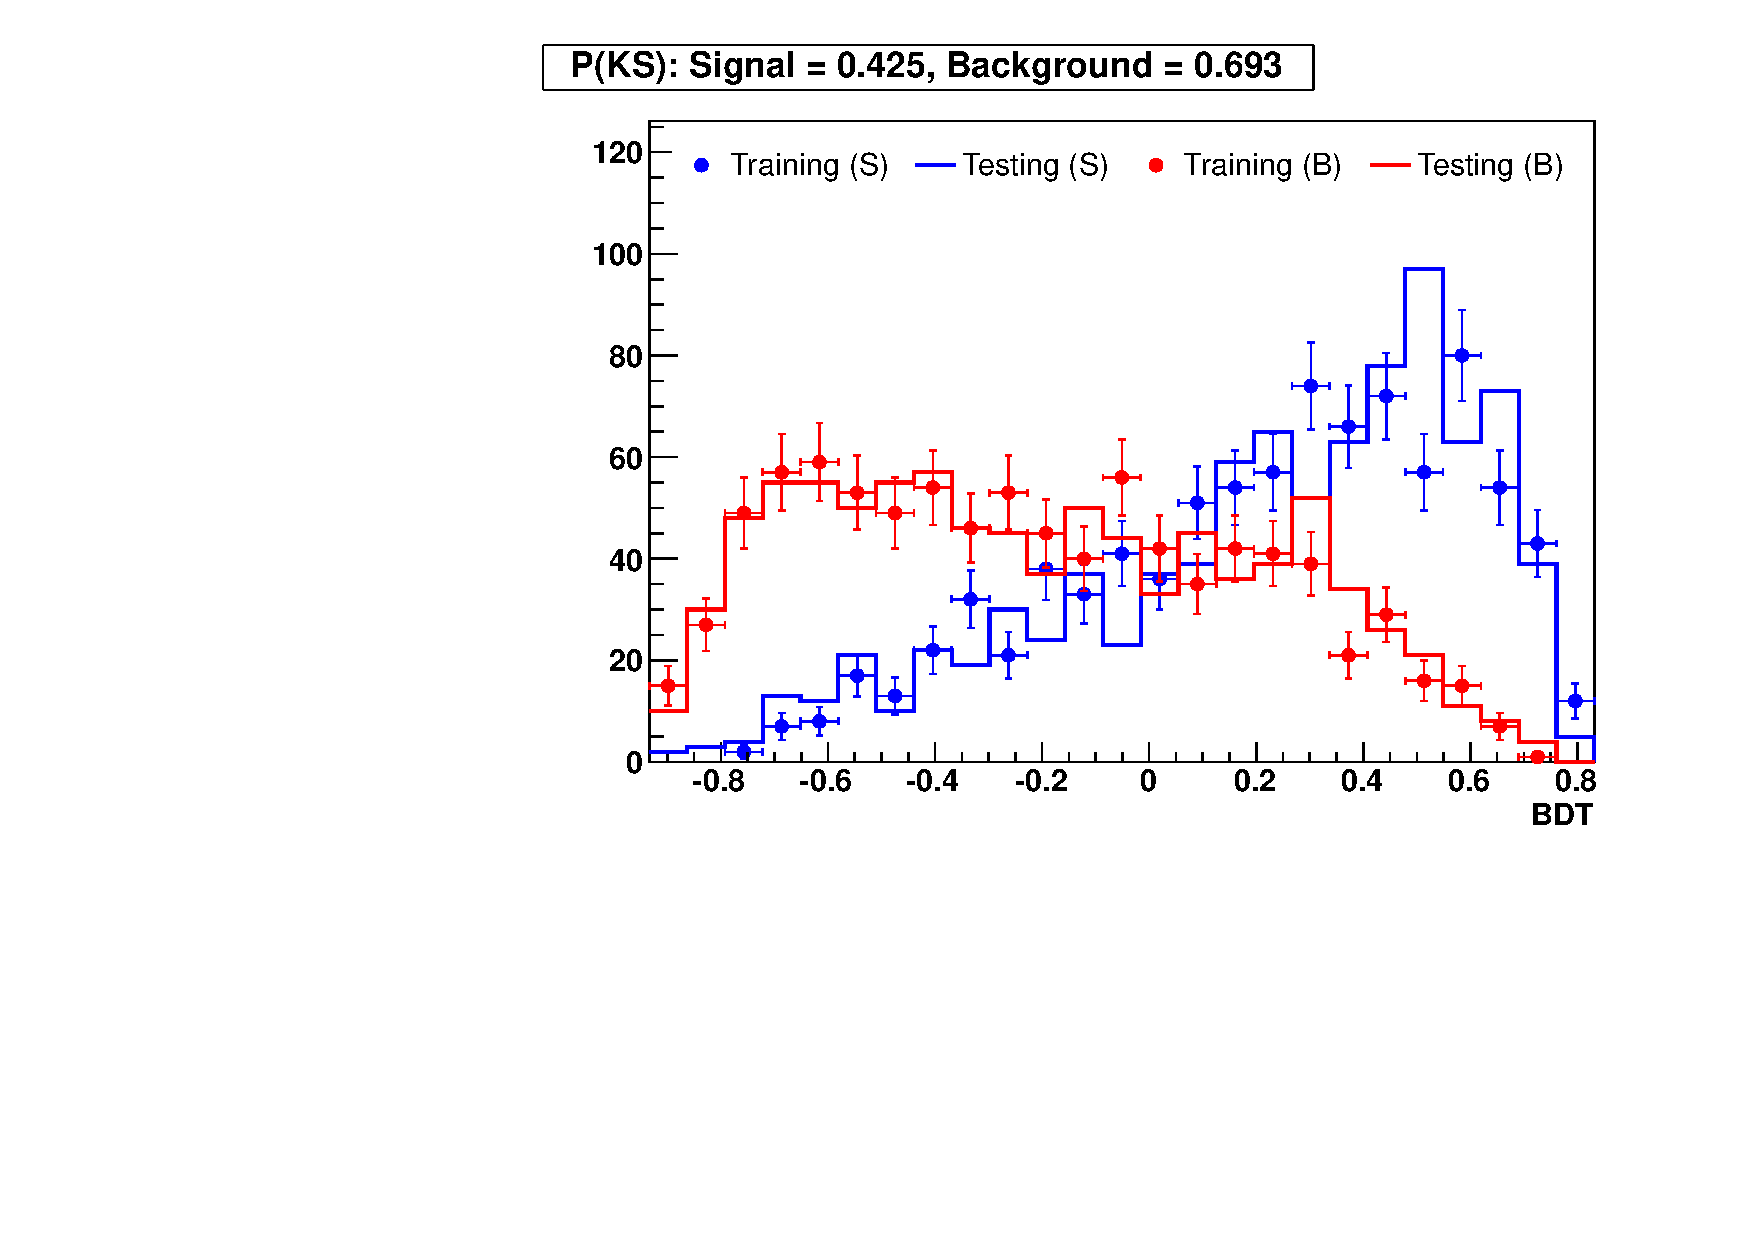
\includegraphics[width=0.45\textwidth]{Figures/Analysis_2_Diagrams/LJ_plots_lep/training/BDT_training_543.pdf}
   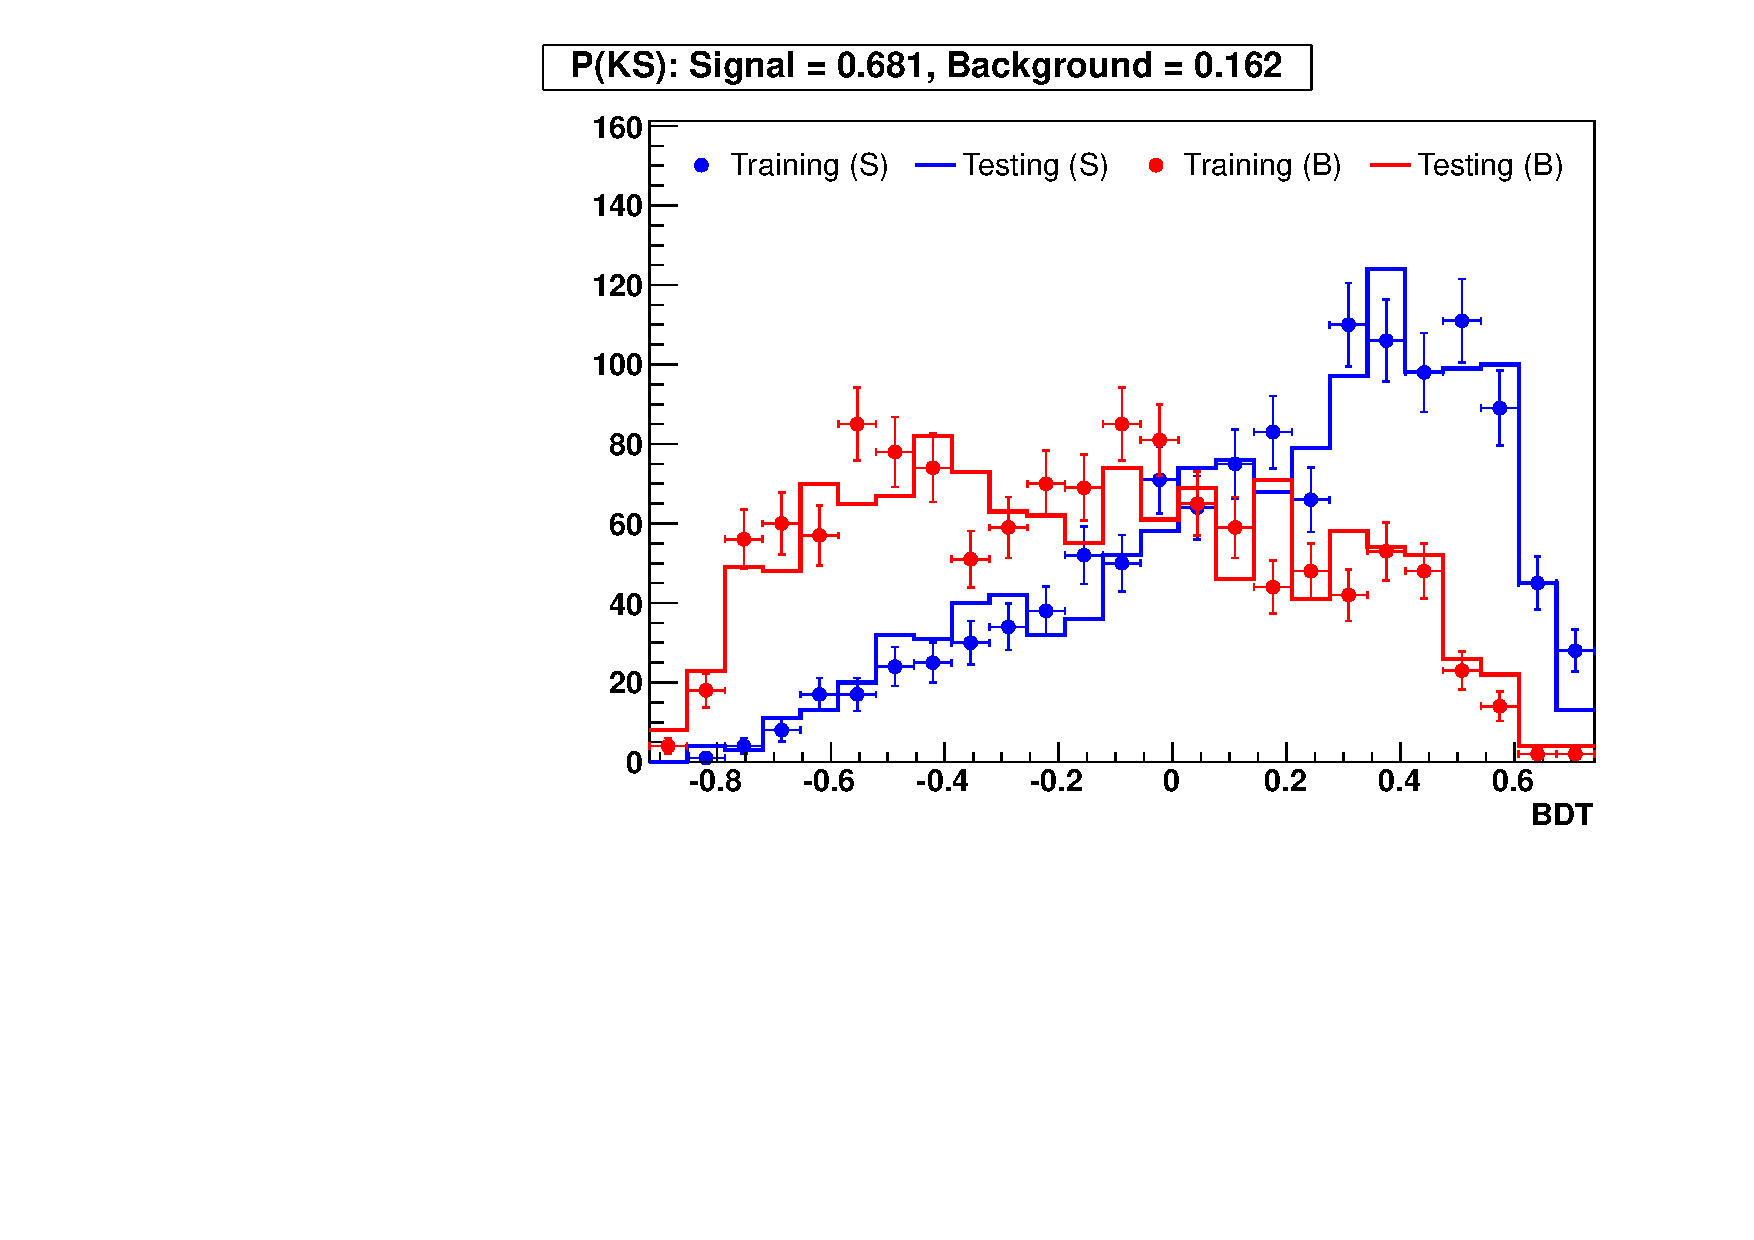
\includegraphics[width=0.45\textwidth]{Figures/Analysis_2_Diagrams/LJ_plots_lep/training/BDT_training_643.pdf}
   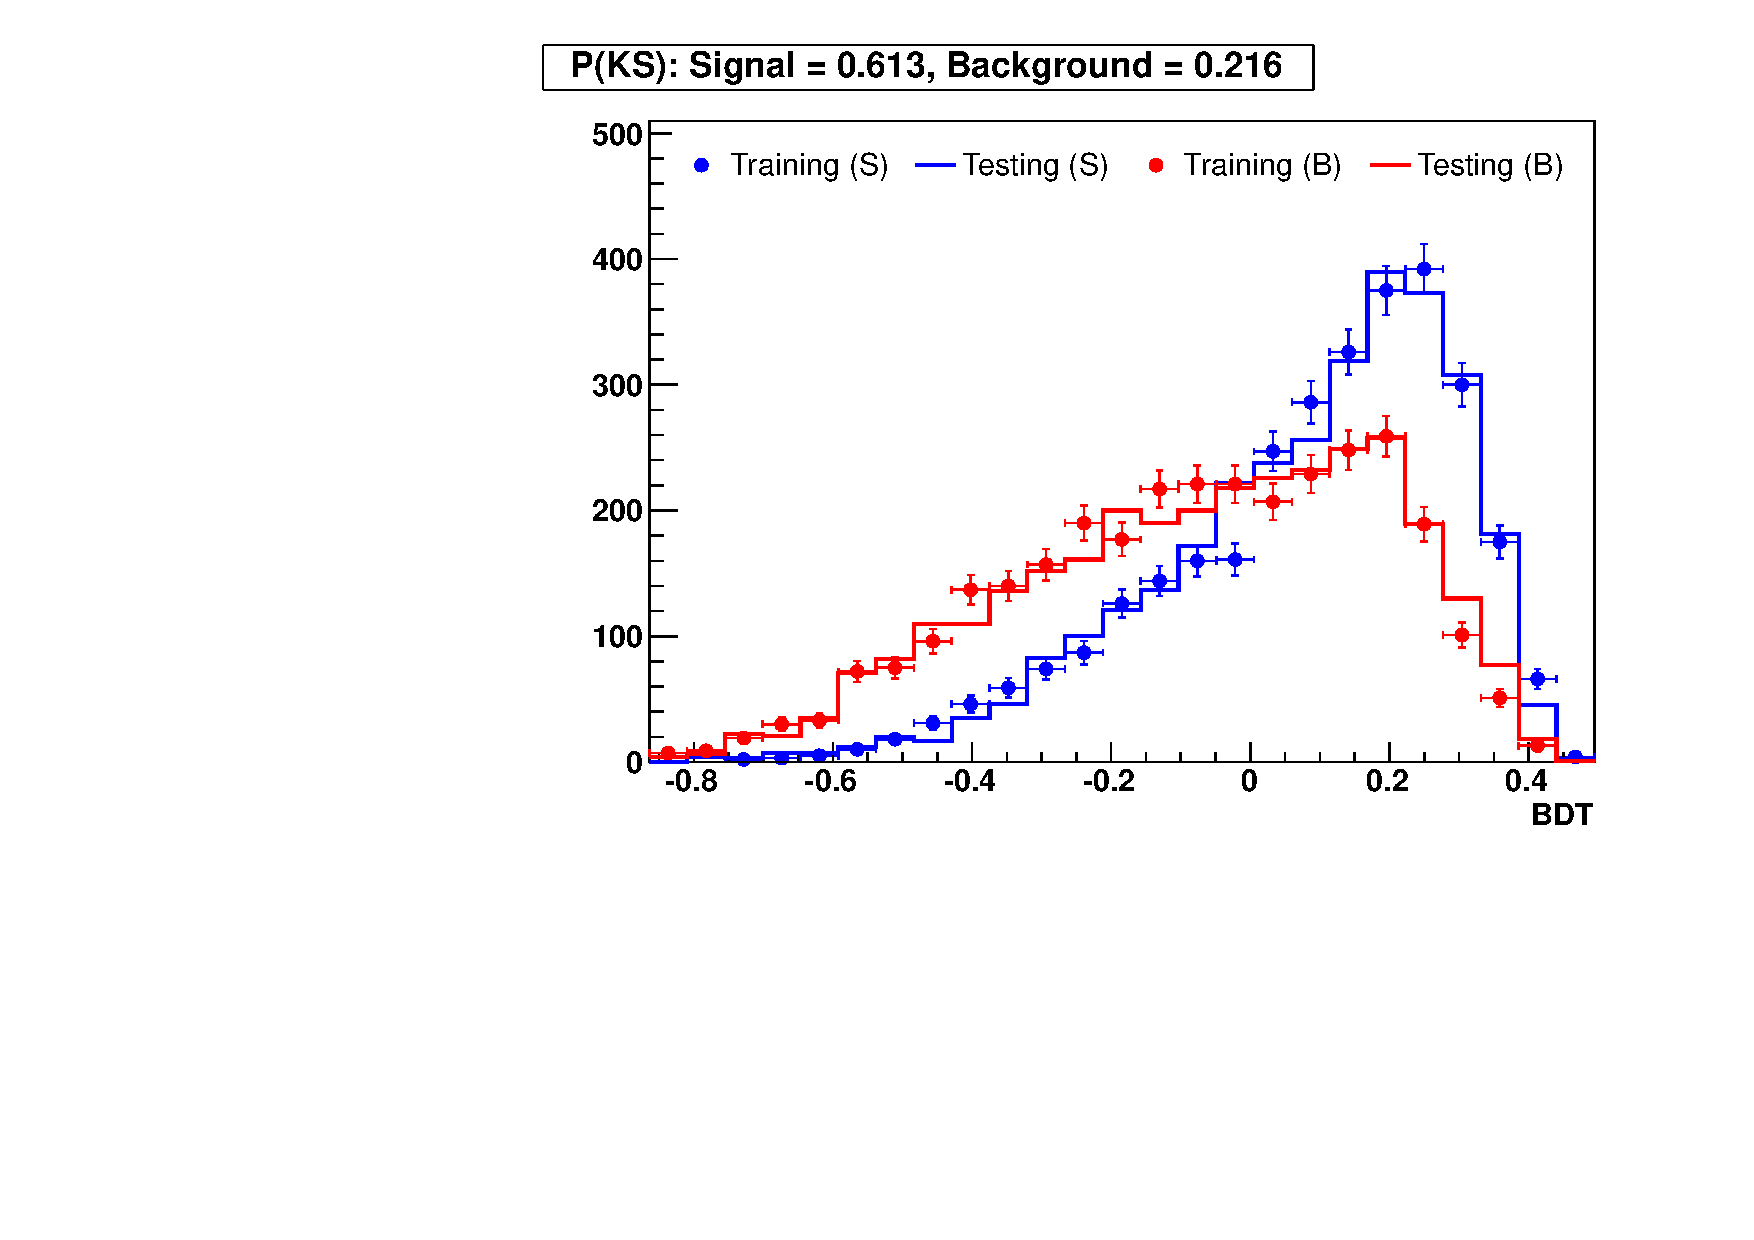
\includegraphics[width=0.45\textwidth]{Figures/Analysis_2_Diagrams/LJ_plots_lep/training/BDT_training_630000.pdf}
   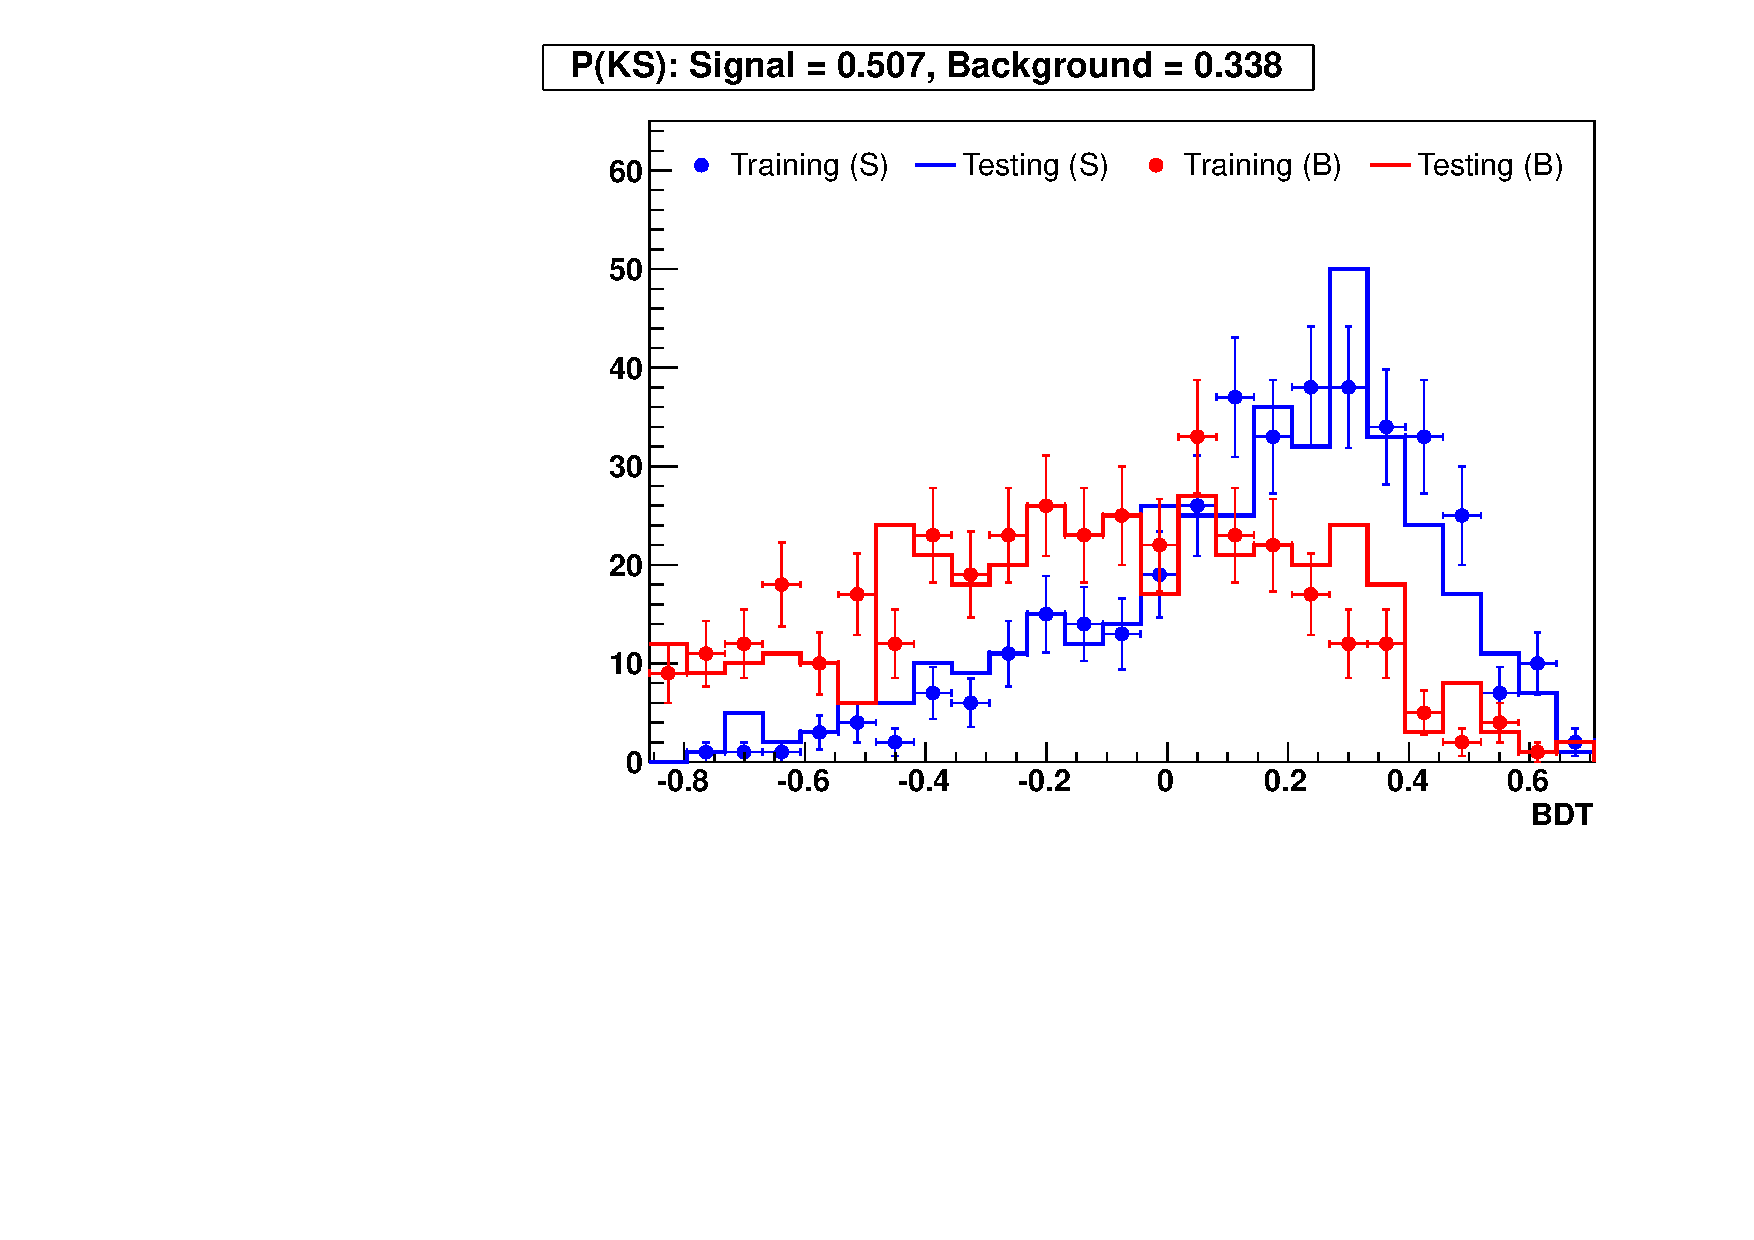
\includegraphics[width=0.45\textwidth]{Figures/Analysis_2_Diagrams/LJ_plots_lep/training/BDT_training_540000.pdf}
   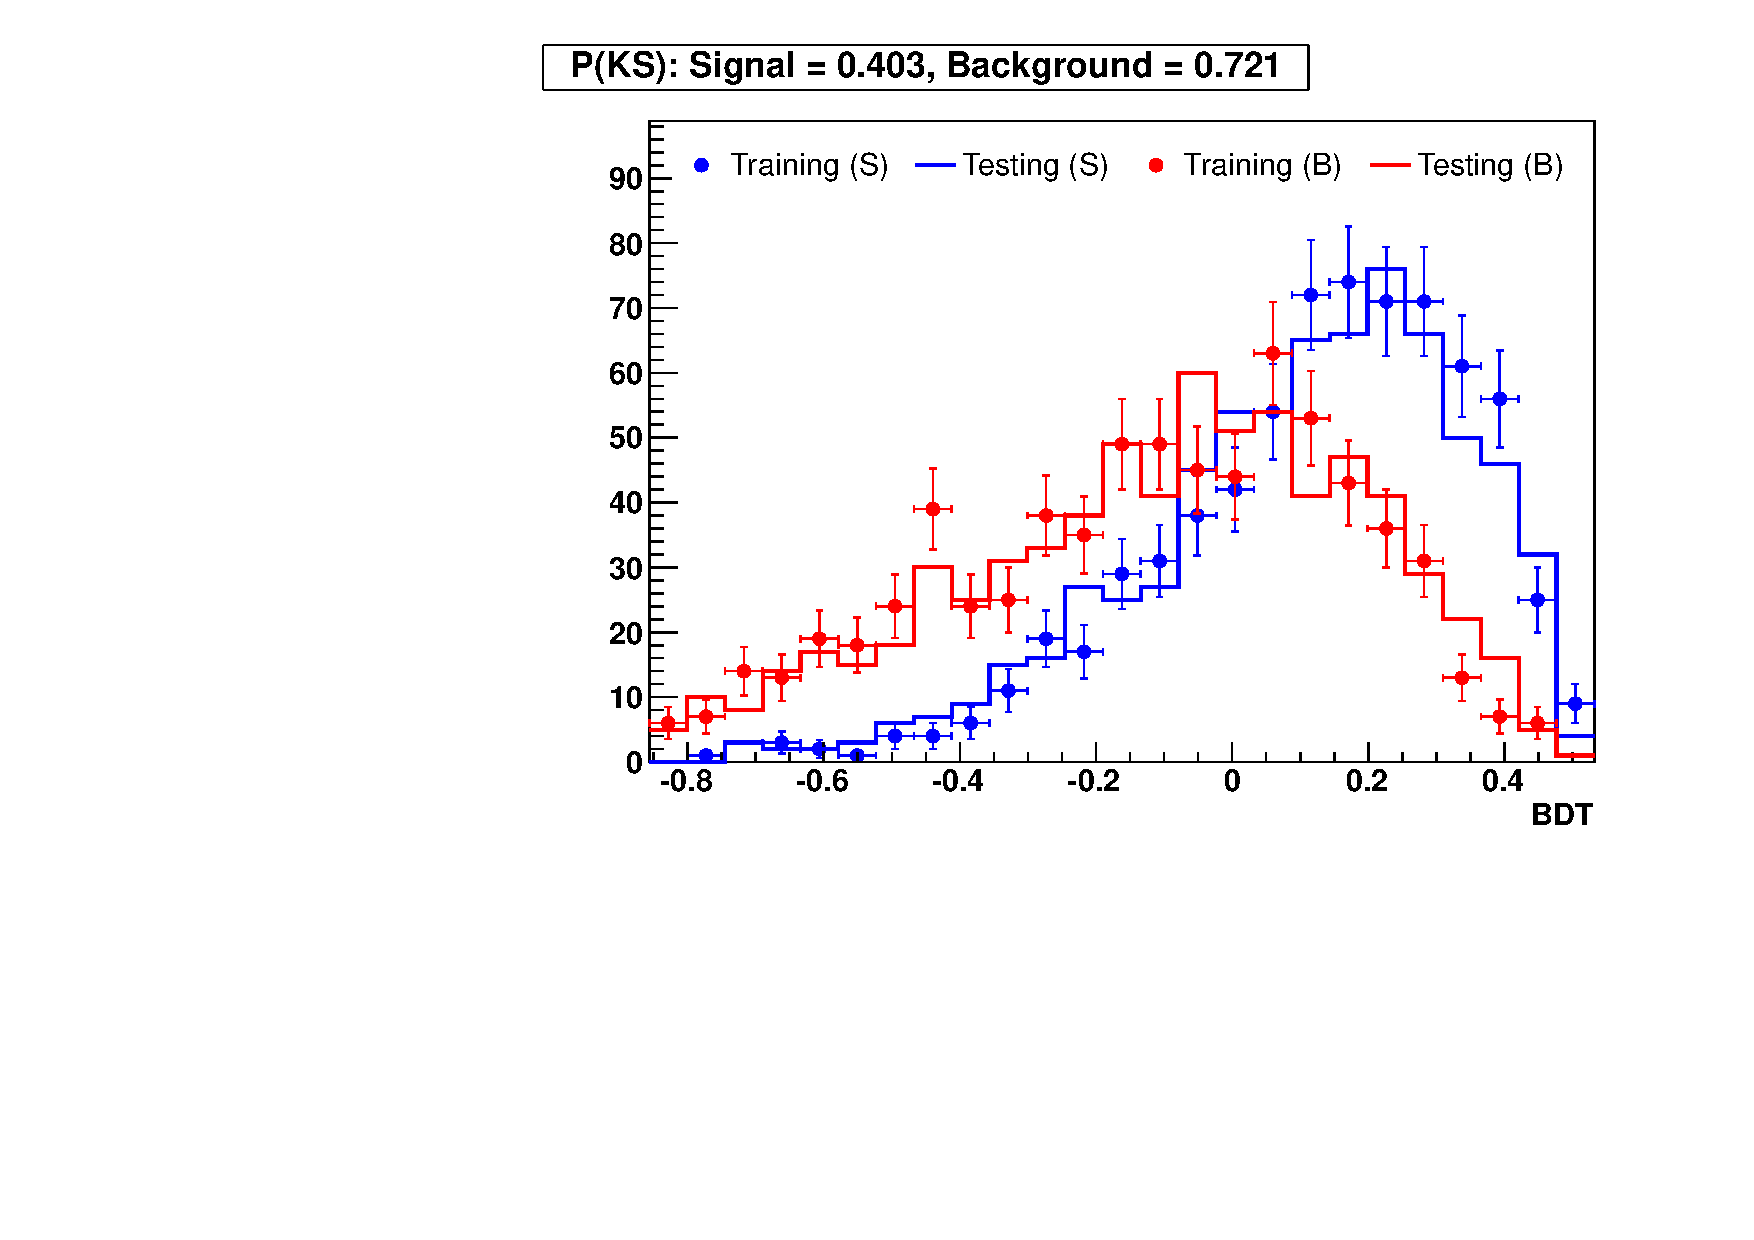
\includegraphics[width=0.45\textwidth]{Figures/Analysis_2_Diagrams/LJ_plots_lep/training/BDT_training_640203.pdf}
      \caption{Comparisons of the testing and training samples used to
      optimize the BDT weights for each jet/tag category}
   \label{fig:bdt_testTrain}
 \end{center}
\end{figure}


\subsection{MVA Input Variables, Data to Monte Carlo Comparisons}
\label{mva_input_vars_data_to_mc_II_overview}

\par The set of 10 input variables for each jet/tag category were
chosen through their ranking using the separation figure of merit
given in equation \ref{eq:separation}.  The categories most sensitive
to signal, 5 jets, $\ge$4 $b$-tags; $\ge$6 jets, $\ge$3 $b$-tags; and
$\ge$6 jets, $\ge$4 $b$-tags all include a variable, which is the
output discriminant of a dedicated BDT trained to separate \ttH signal
from \ttbb background.  Table \ref{tab:bdt_input_vars} gives a
description of each of the input variables used.  Table
\ref{tab:vars_by_category} describes which variables are used in each
jet/tag category, and table \ref{tab:ttbb_tth_disc_input_vars} lists
the variables used in the dedicated \ttH, \ttbb BDT.  

\begin{table}[hbtp]\footnotesize
 \centering 
 \caption{Event variables used in dilepton and lepton+jets BDT training and their descriptions.}
 \label{tab:bdt_input_vars}
 \begin{tabular}{| l | p{10cm} |}
   \hline
   abs \(\Delta \eta\) (leptonic top, bb)      					&  Delta-R between the leptonic top reconstructed by the best Higgs mass algorithm and the $b$-jet pair chosen by the algorithm \\
   abs \(\Delta \eta\) (hadronic top, bb)						&  Delta-R between the hadronic top reconstructed by the best Higgs mass algorithm and the $b$-jet pair chosen by the algorithm \\
   aplanarity  									&  Event shape variable equal to \(\frac{3}{2}(\lambda_{3})\), where \(\lambda_{3}\) is the third eigenvalue of the sphericity tensor as described in~\cite{PhysRevD.1.1416}. \\
   ave CSV (tags/non-tags)    							&  Average $b$-tag discriminant value for $b$-tagged/non-$b$-tagged jets \\
   ave \(\Delta R\)(tag,tag)  							&  Average \(\Delta R\) between $b$-tagged jets \\
   best Higgs mass   								&  A minimum-chi-squared fit to event kinematics is used to select two $b$-tagged jets as top-decay products. Of the remaining $b$-tags, the invariant mass of the two with highest $E_{t}$ is saved. \\
   best \(\Delta R\)(b,b)								& The \(\Delta R\) between the two $b$-jets chosen by the best Higgs mass algorithm \\
   closest tagged dijet mass  							&  The invariant mass of the two $b$-tagged jets that are closest in \(\Delta R\)  \\
   dev from ave CSV (tags)  							&  The square of the difference between the $b$-tag discriminant value of a given $b$-tagged jet and the average $b$-tag discriminant value among $b$-tagged jets, summed over all $b$-tagged jets \\
   highest CSV (tags)  								&  Highest $b$-tag discriminant value among $b$-tagged jets \\
   $H_{0}$, $H_{1}$, $H_{2}$, $H_{3}$  						&  The first few Fox-Wolfram moments ~\cite{tagkey1979543} (event shape variables)  \\
   HT										& Scalar sum of transverse momentum for all jets with \(p_{T}~>~30\) GeV/c \\
\(\sum p_{T}\)(jets,leptons,MET)  						&  The sum of the \(p_{T}\) of all jets, leptons, and MET \\
   \(\sum p_{T}\)(jets,leptons)  							&  The sum of the \(p_{T}\) of all jets, leptons \\
   jet 1, 2, 3, 4 \(p_{T}\)  							&  The transverse momentum of a given jet, where the jet numbers correspond to rank by \(p_{T}\) \\
   % lepton \(p_{T}\)  								&  The transverse momentum of the lepton (LJ channel) \\
   lowest CSV (tags)  								&  Lowest $b$-tag discriminant value among $b$-tagged jets \\
   mass(lepton,jet,MET)  								&  The invariant mass of the 4-vector sum of all jets, leptons, and MET \\
   mass(lepton,closest tag) 							& The invariant mass of the lepton and the closest $b$-tagged jet in \(\Delta R\) \\
   max \(\Delta \eta\) (jet, ave jet \(\eta\))  					&  max difference between jet eta and avg delta eta between jets \\
   max \(\Delta \eta\) (tag, ave jet \(\eta\)) 					&  max difference between tag eta and avg delta eta between jets \\
   max \(\Delta \eta\) (tag, ave tag \(\eta\)) 					&  max difference between tag eta and avg delta eta between tags \\
   median inv. mass (tag pairs)							&  median invariant mass of all combinations of $b$-tag pairs \\
   M3										& The invariant mass of the 3-jet system with the largest transverse momentum. \\
   MHT  										&  Vector sum of transverse momentum for all jets with \(p_{T}~>~30\) GeV/c \\
   MET  										&  Missing transverse energy \\
   min \(\Delta R\)(lepton,jet)  							&  The \(\Delta R\) between the lepton and the closest jet (LJ channel)  \\
   min \(\Delta R\)(tag,tag) 	 						&  The \(\Delta R\) between the two closest $b$-tagged jets \\
   min \(\Delta R\)(jet,jet)  							&  The \(\Delta R\) between the two closest jets \\
   $\sqrt{\Delta \eta(t^{lep}, bb) \times \Delta \eta(t^{had}, bb)}$		&  square root of the product of abs \(\Delta \eta\) (leptonic top, bb) and abs \(\Delta \eta\) (hadronic top, bb) \\
   second-highest CSV (tags)  							&  Second-highest $b$-tag discriminant value among $b$-tagged jets \\
   sphericity  									&  Event shape variable equal to $\frac{3}{2} (\lambda_{2} + \lambda_{3})$, where $\lambda_{2}$ and $\lambda_{3}$ are the second and third eigenvalues of the sphericity tensor as described in~\cite{PhysRevD.1.1416} \\
   (\(\Sigma\) jet \(p_{T}\))/(\(\Sigma\) jet E)					& The ratio of the sum of the transverse momentum of all jets and the sum of the energy of all jets \\
   tagged dijet mass closest to 125						& The invariant mass of the $b$-tagged pair closest to 125 GeV/$c^2$ \\
   \(t\bar{t}b\bar{b}\)/\(t\bar{t}H\) BDT						& BDT used to discriminate between \(t\bar{t}b\bar{b}\) and \(t\bar{t}H\) in the LJ $\geq$ 6 jets, $\geq$ 4 tags, $\geq$6 jets + 3 tags, and 5 jets + $\geq$4 tags categories. See text for description and table~\ref{tab:ttbb_tth_disc_input_vars} for list of variables.\\
   \hline
 \end{tabular}
\end{table}


\begin{table}
\begin{tabular}{ c | c | c |}
% \multicolumn{2}{c|}{}
\cline{2-3}
  &  4 jets, 3 tags  					&  4 jets, 4 tags \\
\cline{2-3}
  &  jet 1 \(p_{T}\)  					&  jet 1 \(p_{T}\)    \\
  &  jet 2 \(p_{T}\) 					&  jet 2 \(p_{T}\)   \\
  &  jet 3 \(p_{T}\)  					&  jet 4 \(p_{T}\)   \\
  &  jet 4 \(p_{T}\)  					&  HT  \\ 
  & M3  						&  \(\sum p_{T}\)(jets,lepton,MET)   \\
  & \(\sum p_{T}\)(jets,lepton,MET)  			&  M3  \\ 
  & HT 							&  ave CSV (tags)   \\
  & lowest CSV (tags)  					&  second-highest CSV (tags) \\
  & MHT   						&  third-highest CSV (tags)  \\
  & MET   						&  lowest CSV (tags)  \\ 
\cline{2-3}

\cline{2-3}
  &  5 jets, 3 tags  					&  5 jets, $\geq$ 4 tags \\
\cline{2-3}
  &  jet 1 \(p_{T}\)   					&  max \(\Delta \eta\) (tag, ave jet \(\eta\))   \\
  &  jet 2 \(p_{T}\)   					&  \(\sum p_{T}\)(jets,lepton,MET)   \\
  &  jet 3 \(p_{T}\)   					&  (\(\Sigma\) jet \(p_{T}\))/(\(\Sigma\) jet E)   \\
  & jet 4 \(p_{T}\)  					&  ave \(\Delta R\)(tag,tag)   \\
  & \(\sum p_{T}\)(jets,lepton,MET) 			&  ave CSV (tags)   \\
  & (\(\Sigma\) jet \(p_{T}\))/(\(\Sigma\) jet E)   	&  dev from ave CSV (tags)   \\
  &  HT  						&  second-highest CSV (tags)   \\
  &  ave CSV (tags)  					& third-highest CSV (tags)   \\
  & third-highest CSV (tags) 				& lowest CSV (tags) \\
  &  fourth-highest CSV (jets)  			& ttbb/ttH BDT \\
\cline{2-3}

\hline
  \multicolumn{1}{|c|}{$\geq$ 6 jets, 2 tags}  				& $\geq$ 6 jets, 3 tags  			&  $\geq$ 6 jets, $\geq$ 4 tags \\
\hline
  \multicolumn{1}{|c|}{\(\sum p_{T}\)(jets,lepton,MET)}  		&  $H_{0}$  					&  (\(\Sigma\) jet \(p_{T}\))/(\(\Sigma\) jet E) \\
  \multicolumn{1}{|c|}{HT}  						&  sphericity					&  ave \(\Delta R\)(tag,tag) \\
  \multicolumn{1}{|c|}{mass(lepton,closest tag)} 			&  (\(\Sigma\) jet \(p_{T}\))/(\(\Sigma\) jet E)&  product(\(\Delta \eta\)(leptonic top, bb), \(\Delta \eta\)(hadronic top, bb)) \\
  \multicolumn{1}{|c|}{max \(\Delta \eta\) (jet, ave jet \(\eta\))}  	&  max \(\Delta \eta\) (jet, ave jet \(\eta\)) 	&  closest tag mass \\
  \multicolumn{1}{|c|}{min \(\Delta R\)(lepton,jet)} 			&  \(\sum p_{T}\)(jets,lepton,MET)  		&  max \(\Delta \eta\) (tag, ave tag \(\eta\)) \\
  \multicolumn{1}{|c|}{\(H_{2}\)} 					&  ave CSV (tags)  				&  ave CSV (tags) \\
  \multicolumn{1}{|c|}{sphericity} 					&  second-highest CSV (tags)			&  third-highest CSV (tags) \\
  \multicolumn{1}{|c|}{(\(\Sigma\) jet \(p_{T}\))/(\(\Sigma\) jet E)} 	&  third-highest CSV (tags) 			&  fourth-highest CSV (tags) \\
  \multicolumn{1}{|c|}{third-highest CSV (jets)} 			&  fourth-highest CSV (jets)  			&  best Higgs mass \\
  \multicolumn{1}{|c|}{fourth-highest CSV (jets)} 			&  ttbb/ttH BDT  				&  ttbb/ttH BDT \\

\hline
\end{tabular}
\caption{BDT input variable assignments for the lepton+jets categories.}
\label{tab:vars_by_category}
\end{table}



\begin{table}[hbtp]\footnotesize
  \centering
  \begin{tabular}{| c | c | c |}
    \hline
    5 jets, $\geq$ 4 tags						&  $\geq$ 6 jets, 3 tags						&  $\geq$ 6 jets, $\geq$ 4 tags \\				                       
    \hline																									                       
    ave \(\Delta R\)(tag,tag)    	    				& tagged dijet mass closest to 125					&  $H_{3}$ \\						                               
    max \(\Delta \eta\) (tag, ave tag \(\eta\))    	    		& (\(\Sigma\) jet \(p_{T}\))/(\(\Sigma\) jet E)				&  ave \(\Delta R\)(tag,tag) \\				                               
(\(\Sigma\) jet \(p_{T}\))/(\(\Sigma\) jet E)    	    	& $\sqrt{\Delta \eta(t^{lep}, bb) \times \Delta \eta(t^{had}, bb)}$	&  closest tagged dijet mass \\				                               
tagged dijet mass closest to 125    	    			& $H_{1}$								&  sphericity \\						                       
$H_{1}$    	    						& $H_{3}$								&  max \(\Delta \eta\) (tag, ave jet \(\eta\)) \\		                       
$H_{3}$    	    						& M3									&  max \(\Delta \eta\) (tag, ave tag \(\eta\)) \\		                       
\(\sum p_{T}\)(jets,lepton,MET)    	    			& max \(\Delta \eta\) (tag, ave tag \(\eta\))				&  mass(lepton,jet,MET) \\  				                               
fourth-highest CSV (tags)    	    				& max \(\Delta \eta\) (tag, ave jet \(\eta\))				&  (\(\Sigma\) jet \(p_{T}\))/(\(\Sigma\) jet E) \\ 	                               
aplanarity    	    						& max \(\Delta \eta\) (jet, ave jet \(\eta\))				&  abs \(\Delta \eta\) (leptonic top, bb) \\			                       
MET    	    							& abs \(\Delta \eta\) (hadronic top, bb)				&  abs \(\Delta \eta\) (hadronic top, bb) \\			                       
 	    							& abs \(\Delta \eta\) (leptonic top, bb)				&  $\sqrt{\Delta \eta(t^{lep}, bb) \times \Delta \eta(t^{had}, bb)}$ \\                
     	    							& sphericity								&  ave CSV (tags) \\					                               
     	    							& aplanarity								&  best \(\Delta R\)(b,b) \\				                               
     	    							& min \(\Delta R\)(tag,tag)						&  best Higgs mass \\					                               
     	   	 						& jet 3 \(p_{T}\)							&  median inv. mass (tag pairs) \\  			                               
\hline
\end{tabular}
\caption{List of variables used as inputs in each of the ttbb/ttH BDTs. See table~\ref{tab:bdt_input_vars} for definitions.}
\label{tab:ttbb_tth_disc_input_vars}
\end{table}


\par The modeling of the input variables is compared against data for
each of the jet/tag diagrams in the the following figures: 

\begin{itemize}
  \item $\ge$6 jets,  $==$2 $b$-tags: Figure
    \ref{fig:lj_input_II_6j2t}
  \item $==$4 jets, $==$3 $b$-tags: Figure
    \ref{fig:lj_input_II_4j3t}
  \item $==$5 jets, $==$3 $b$-tags: Figure
    \ref{fig:lj_input_II_5j3t}
  \item $\ge$6 jets, $==$3 $b$-tags: Figure
    \ref{fig:lj_input_II_6j3t_1}, and Figure \ref{fig:lj_input_II_6j3t_2}
  \item $==$4 jets, $==$4 $b$-tags: Figure
    \ref{fig:lj_input_II_4j4t}
  \item $==$5 jets, $==$4 $b$-tags: Figure
    \ref{fig:lj_input_II_5j4t_1}, and Figure \ref{fig:lj_input_II_5j4t_2}
  \item $\ge$6 jets, $\ge$4 $b$-tags: Figure
    \ref{fig:lj_input_II_6j4t_1}, and Figure \ref{fig:lj_input_II_6j4t_2}
\end{itemize}


\begin{figure}[hbtp]
 \begin{center}
   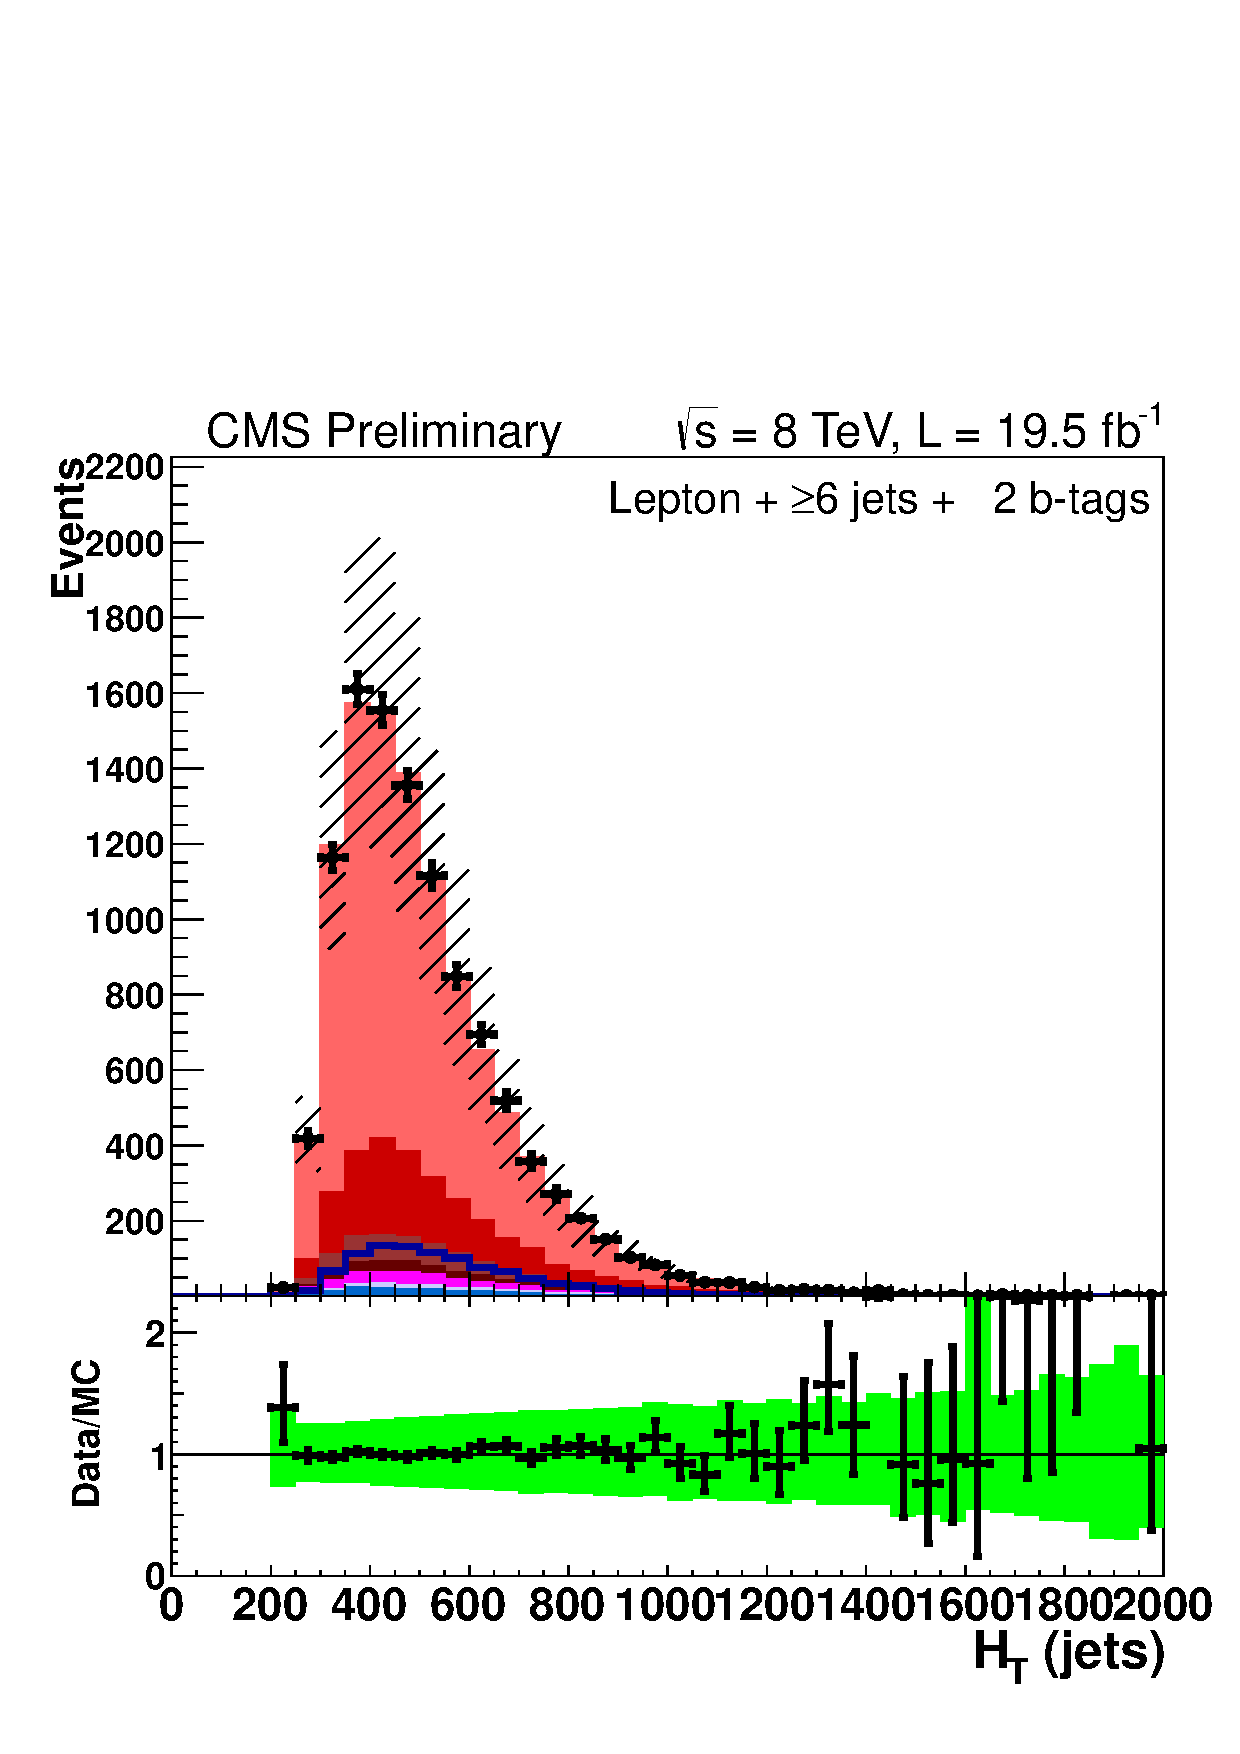
\includegraphics[width=0.31\textwidth]{Figures/Analysis_2_Diagrams/LJ_plots_lep/6j2t/lep_HT_6j2t_cumulative_wRatio_noLegend_lin.pdf}
   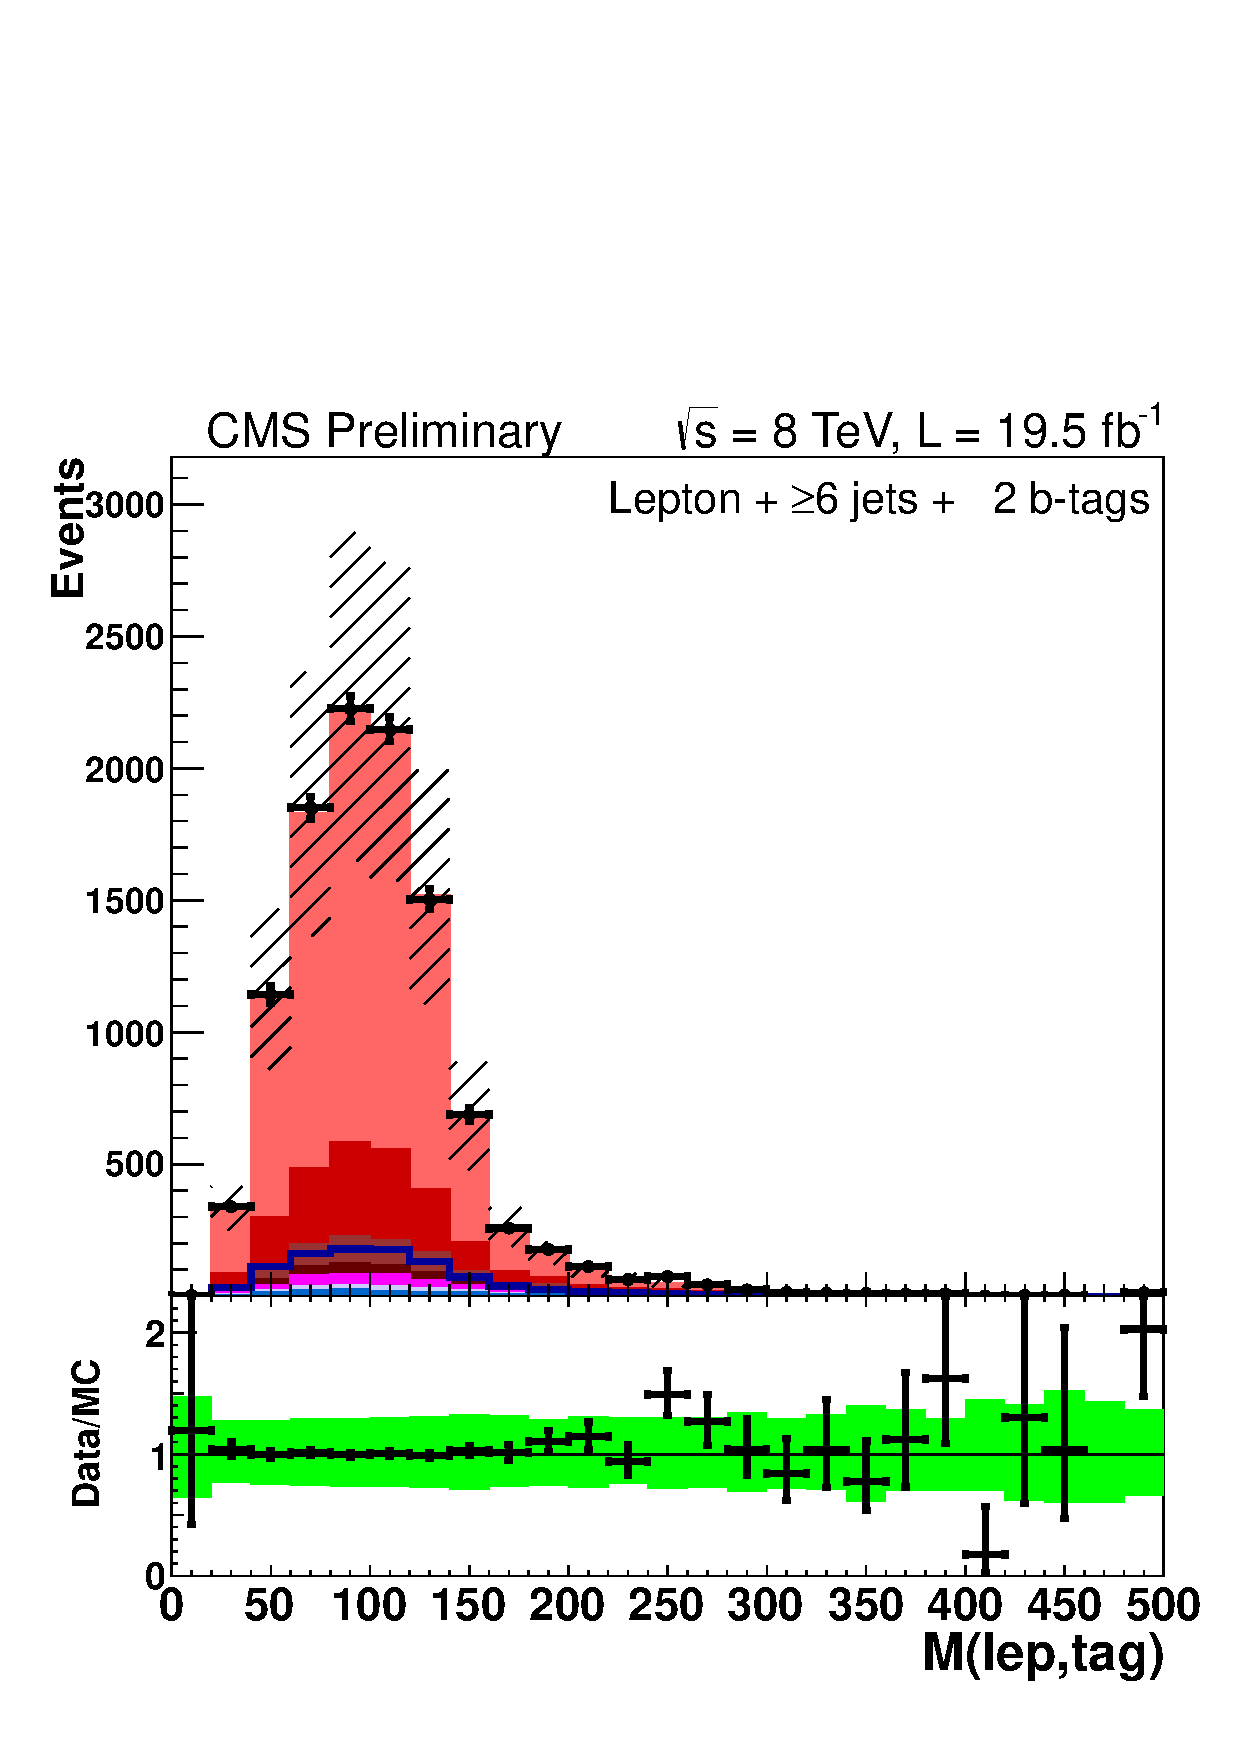
\includegraphics[width=0.31\textwidth]{Figures/Analysis_2_Diagrams/LJ_plots_lep/6j2t/lep_Mlb_6j2t_cumulative_wRatio_noLegend_lin.pdf}
   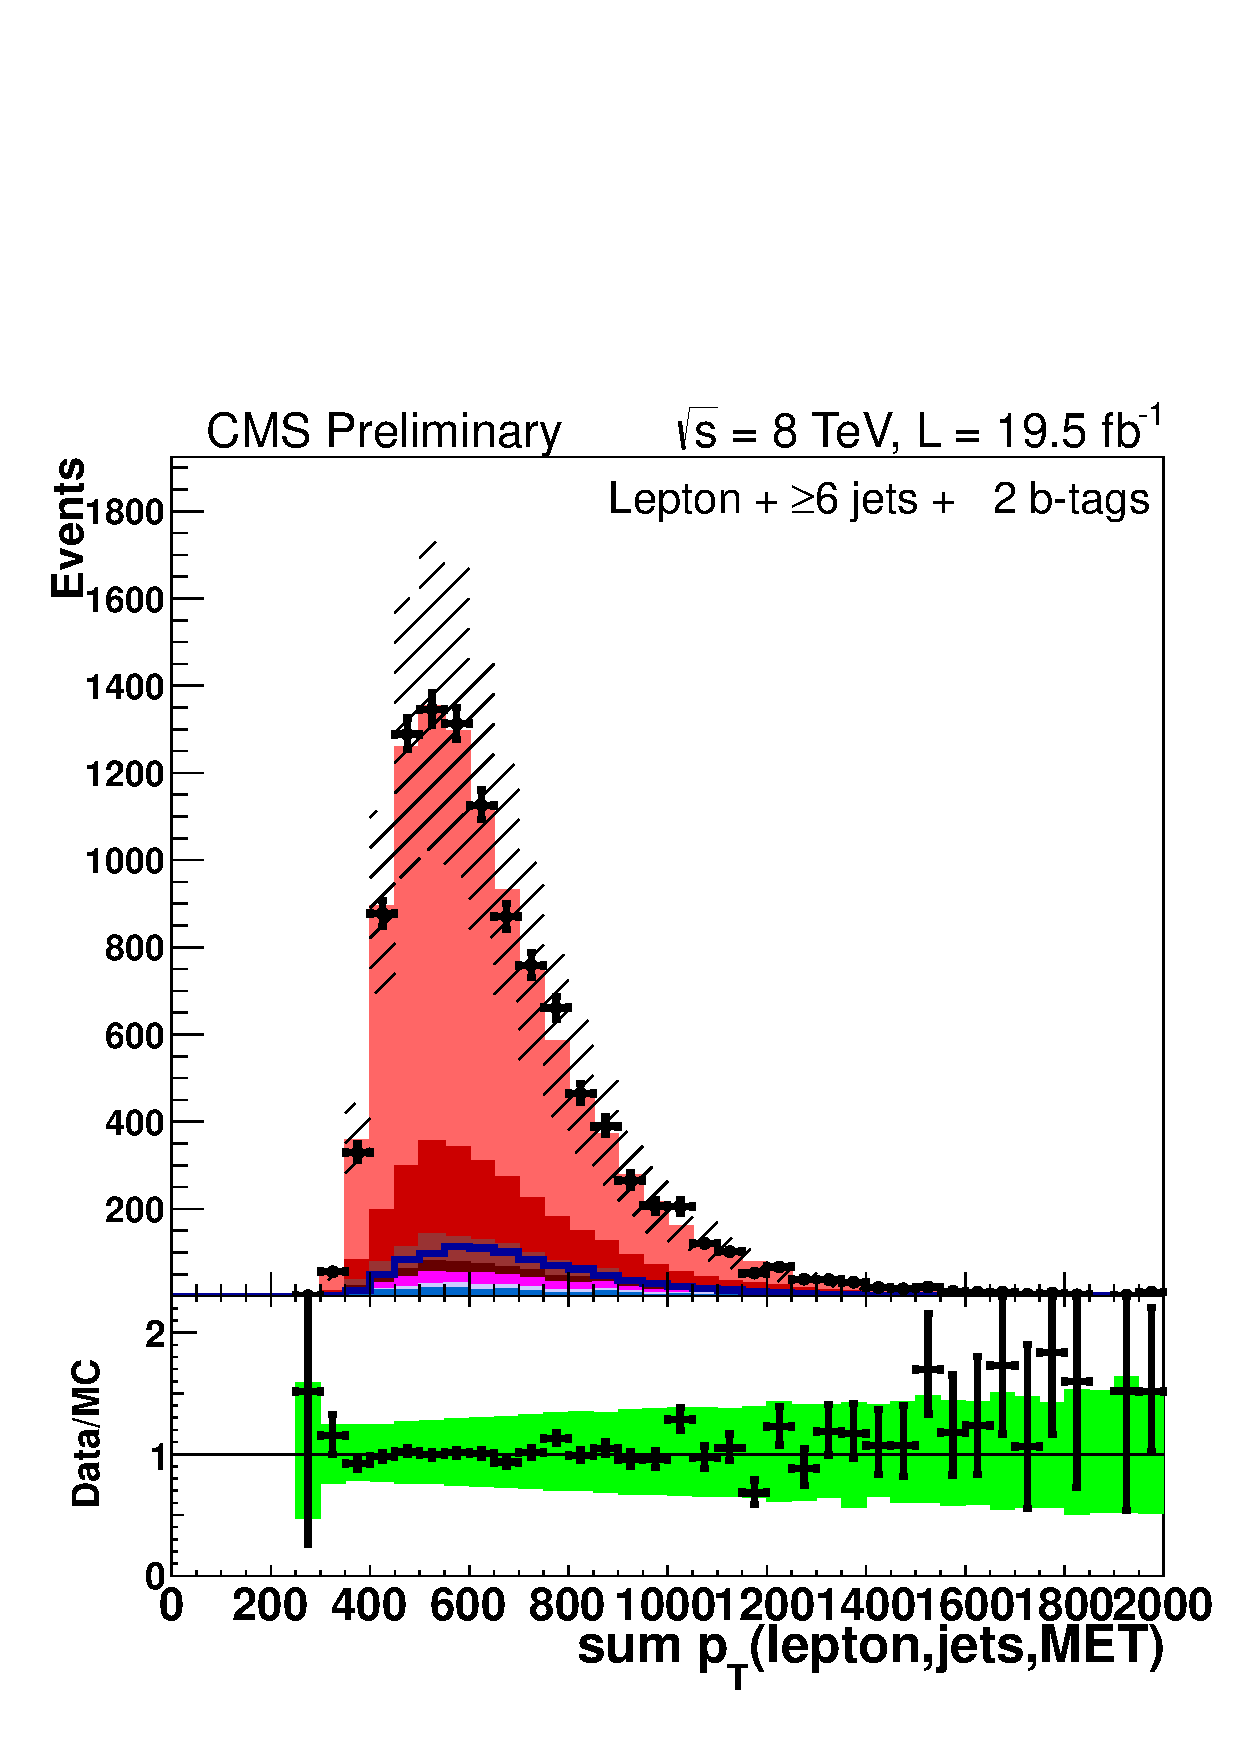
\includegraphics[width=0.31\textwidth]{Figures/Analysis_2_Diagrams/LJ_plots_lep/6j2t/lep_all_sum_pt_with_met_6j2t_cumulative_wRatio_noLegend_lin.pdf}
   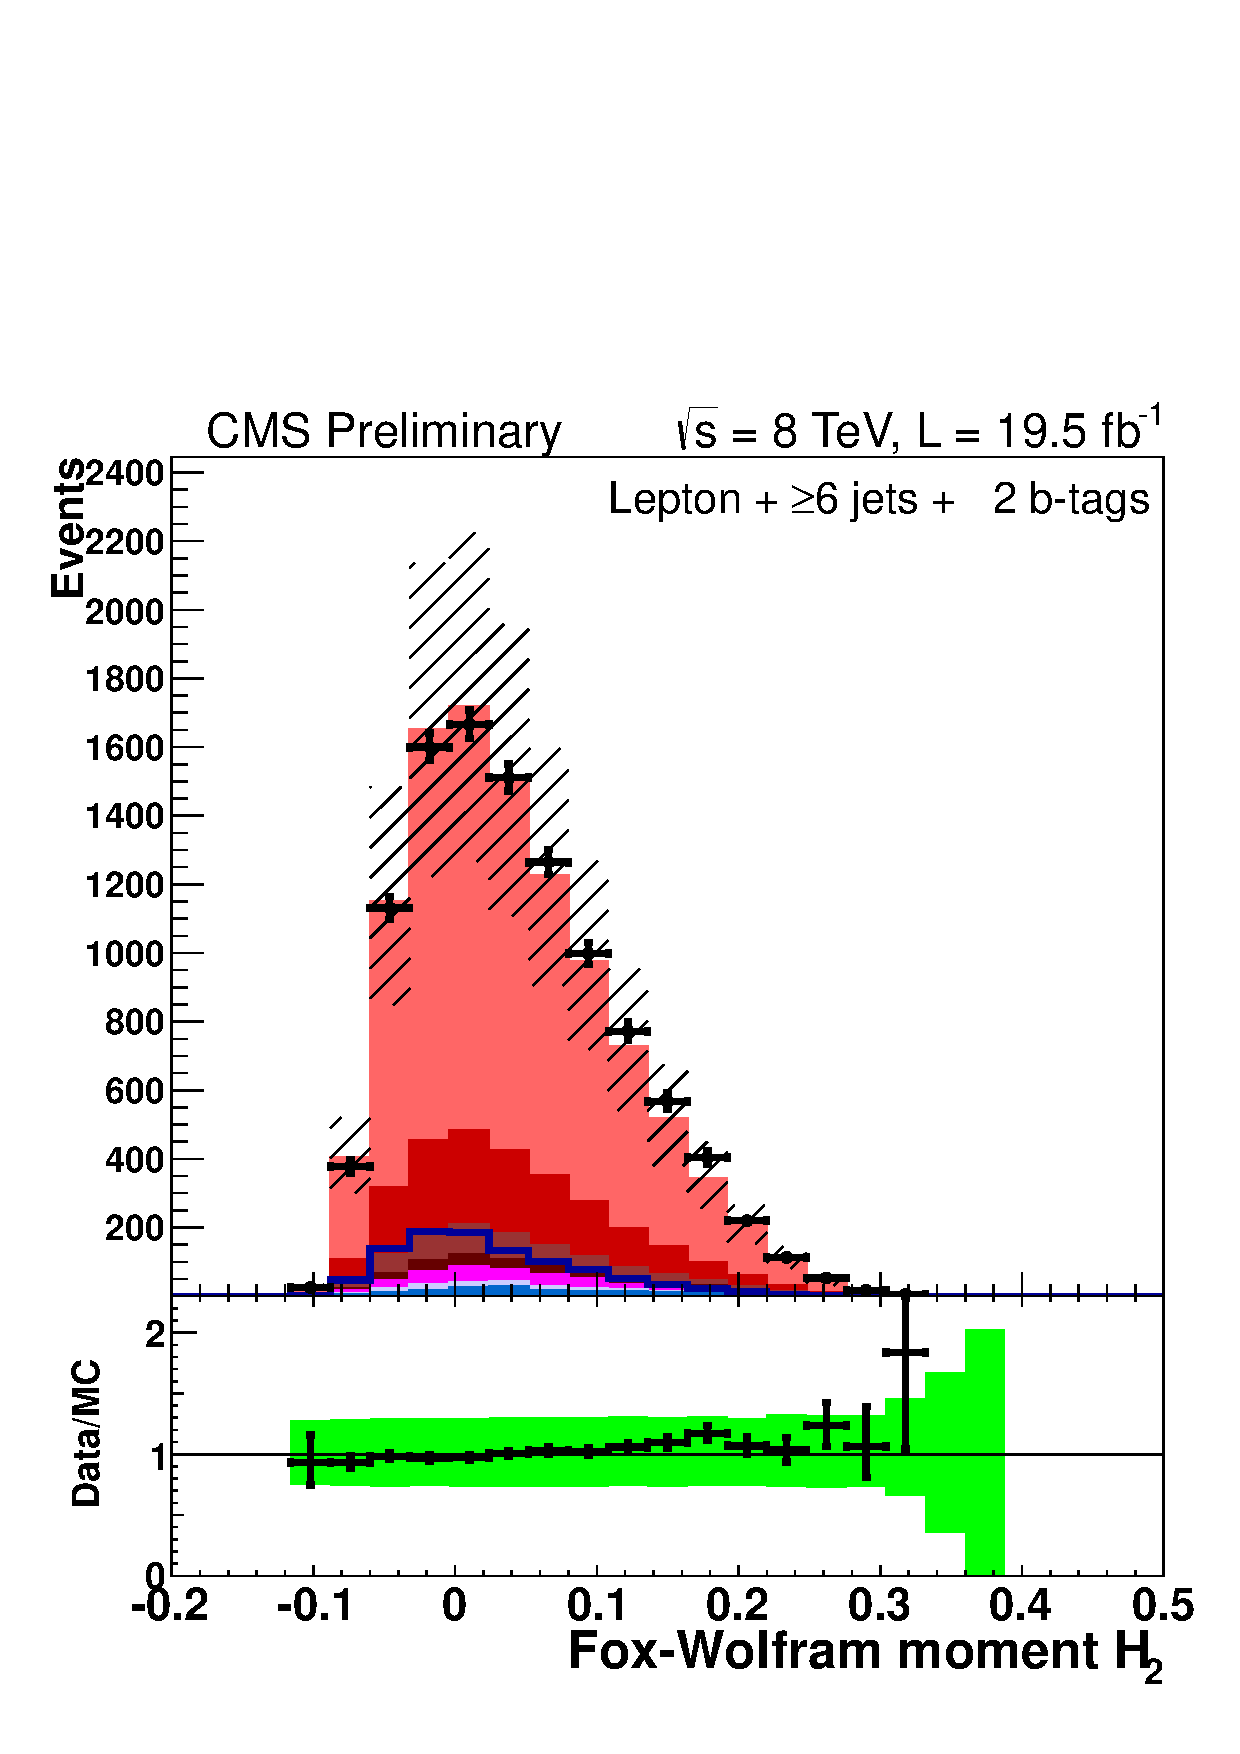
\includegraphics[width=0.31\textwidth]{Figures/Analysis_2_Diagrams/LJ_plots_lep/6j2t/lep_h2_6j2t_cumulative_wRatio_noLegend_lin.pdf}
   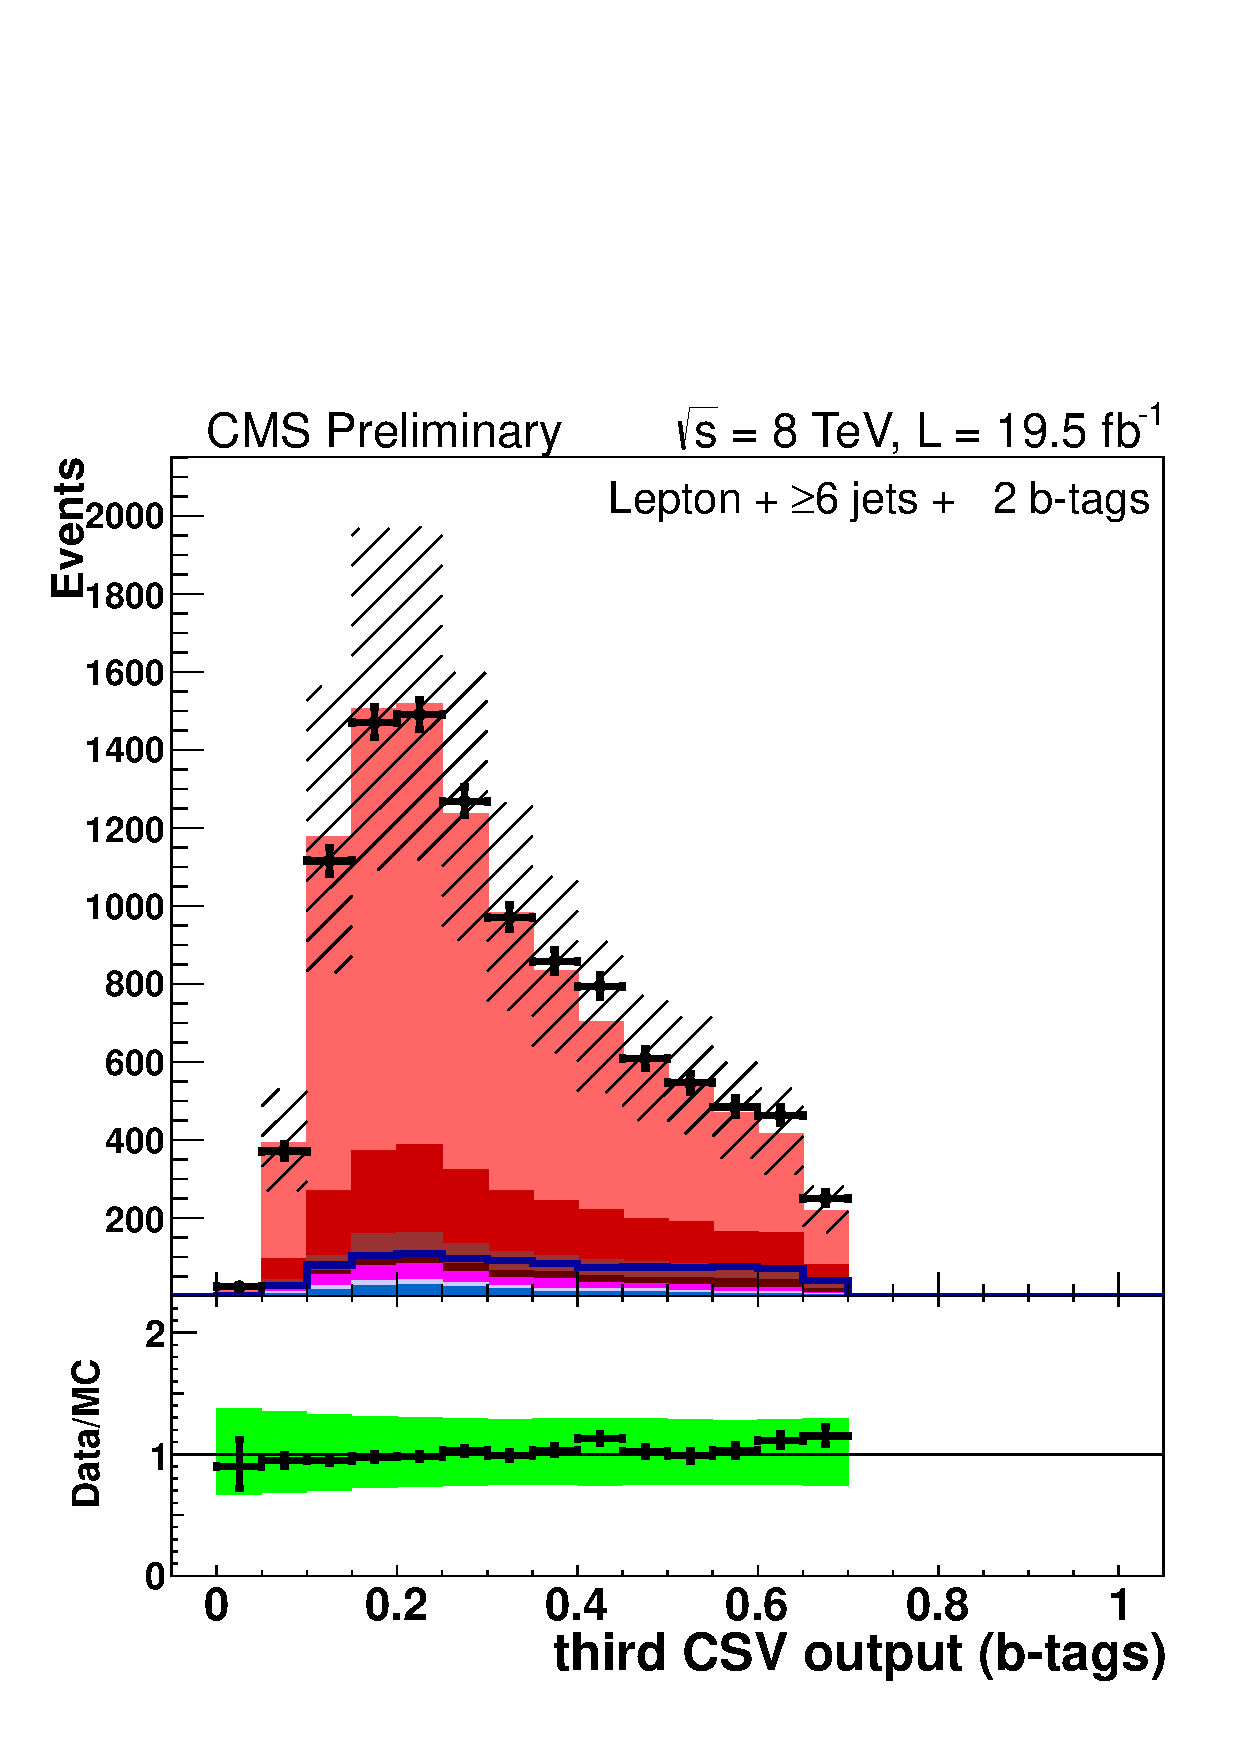
\includegraphics[width=0.31\textwidth]{Figures/Analysis_2_Diagrams/LJ_plots_lep/6j2t/lep_jet_csv_3_6j2t_cumulative_wRatio_noLegend_lin.pdf}
   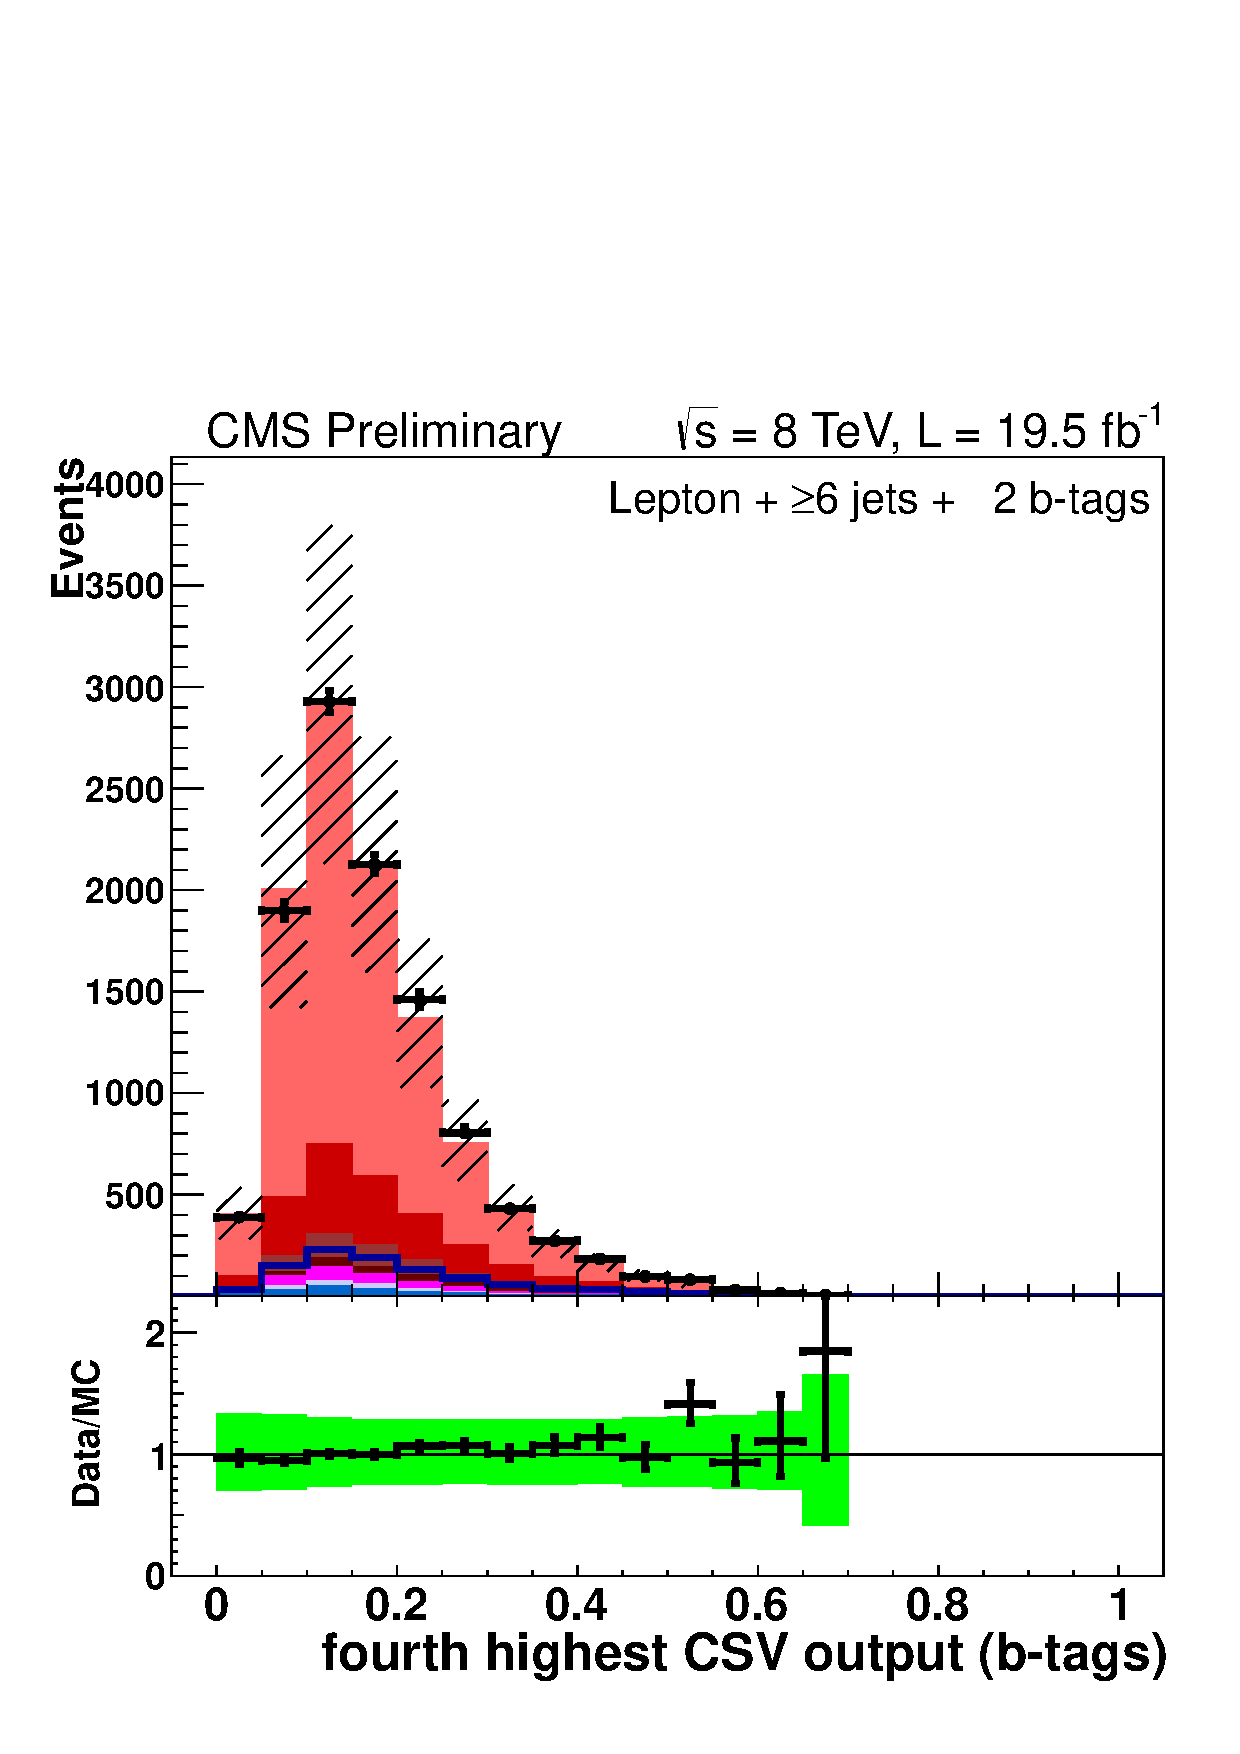
\includegraphics[width=0.31\textwidth]{Figures/Analysis_2_Diagrams/LJ_plots_lep/6j2t/lep_jet_csv_4_6j2t_cumulative_wRatio_noLegend_lin.pdf}
   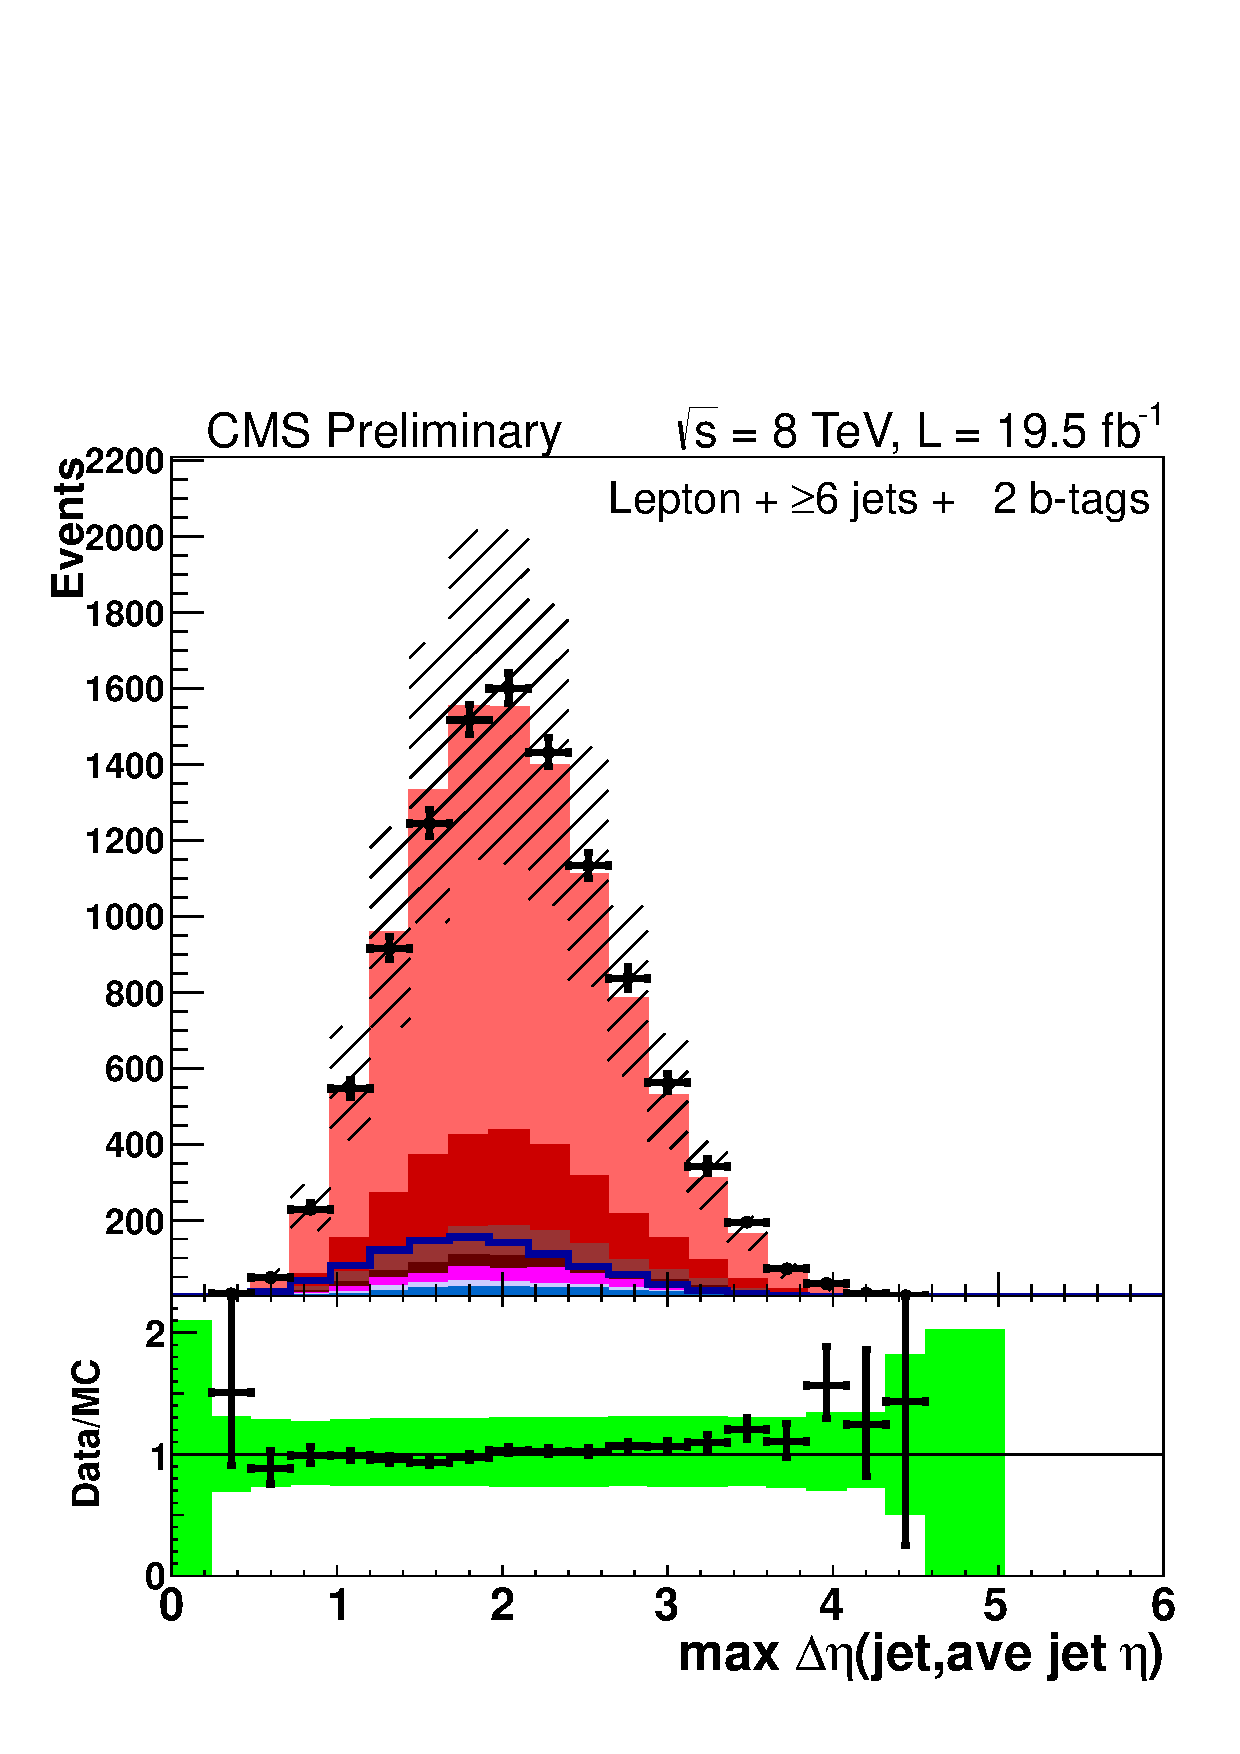
\includegraphics[width=0.31\textwidth]{Figures/Analysis_2_Diagrams/LJ_plots_lep/6j2t/lep_maxeta_jet_jet_6j2t_cumulative_wRatio_noLegend_lin.pdf}
   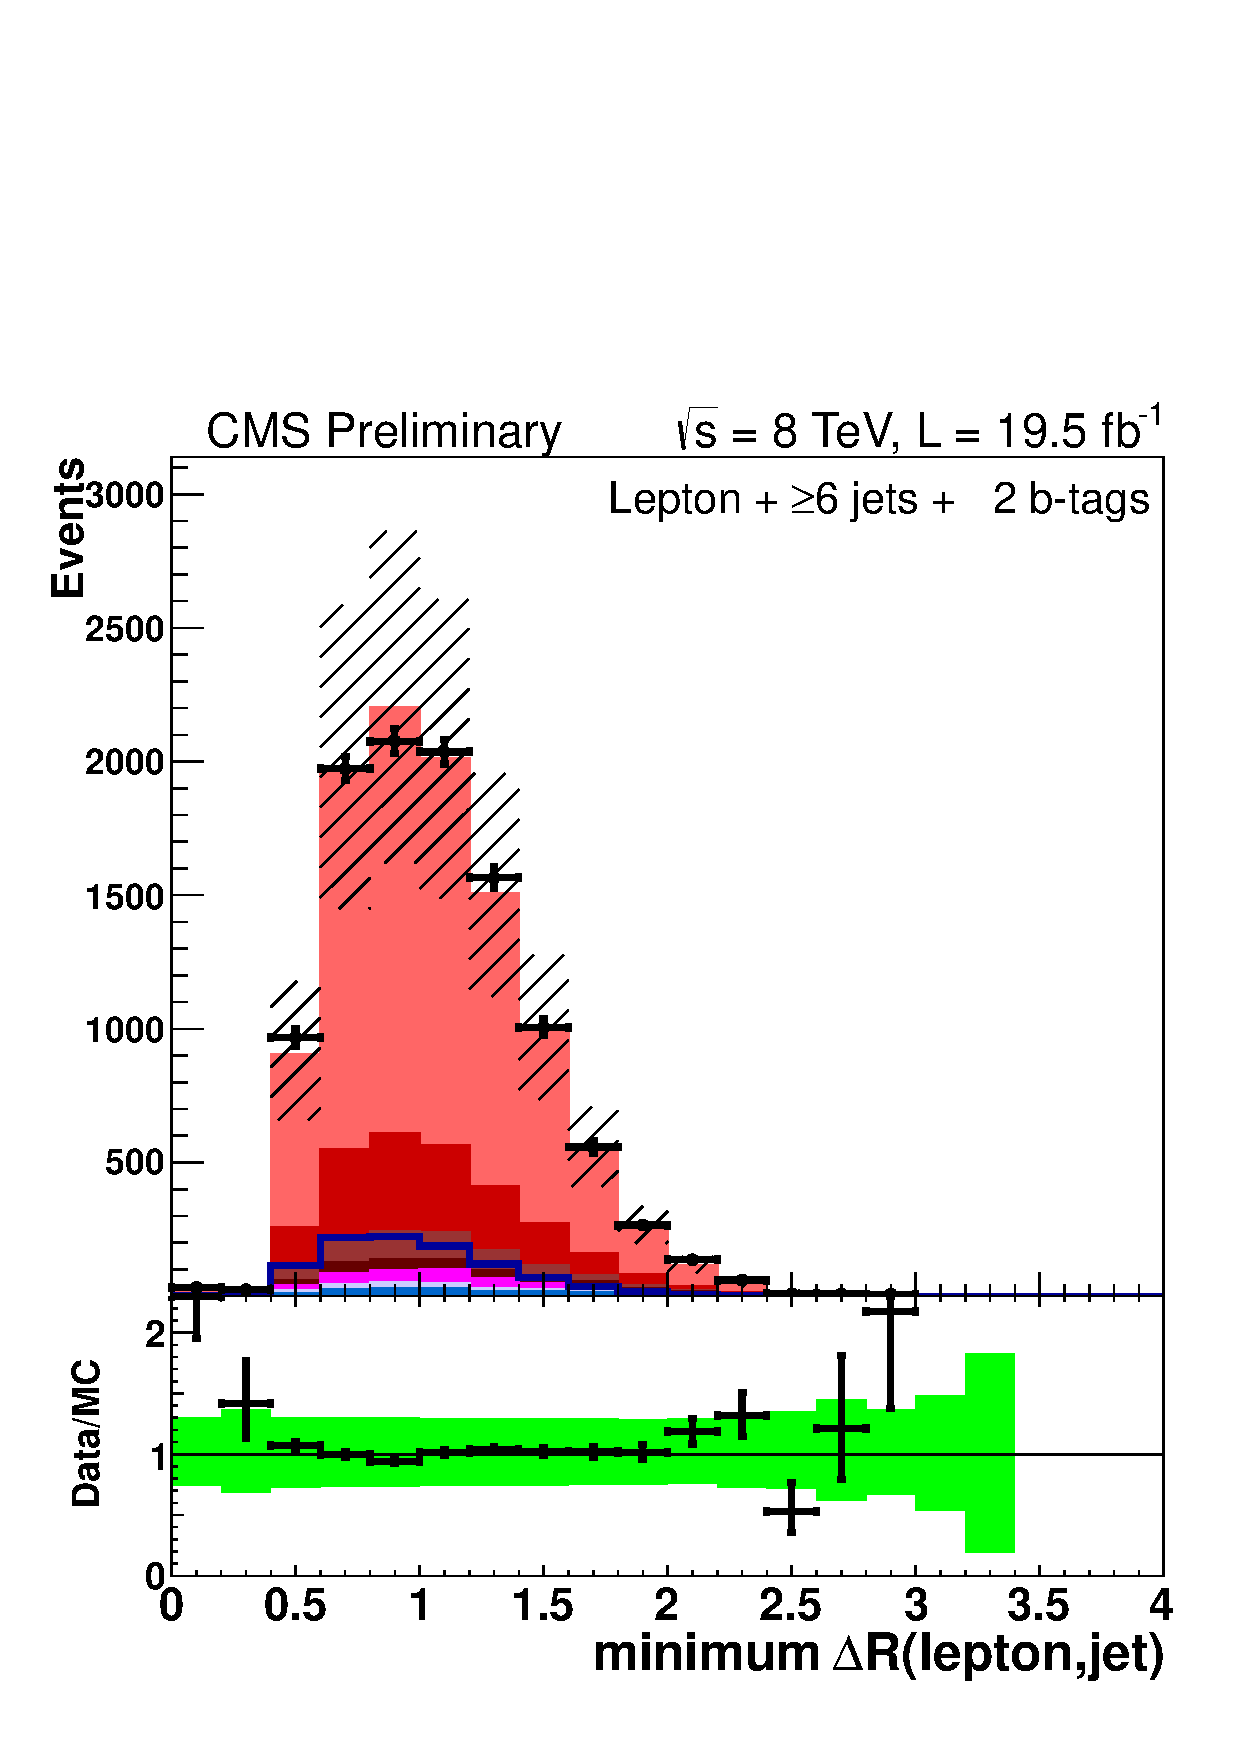
\includegraphics[width=0.31\textwidth]{Figures/Analysis_2_Diagrams/LJ_plots_lep/6j2t/lep_min_dR_lep_jet_6j2t_cumulative_wRatio_noLegend_lin.pdf}
   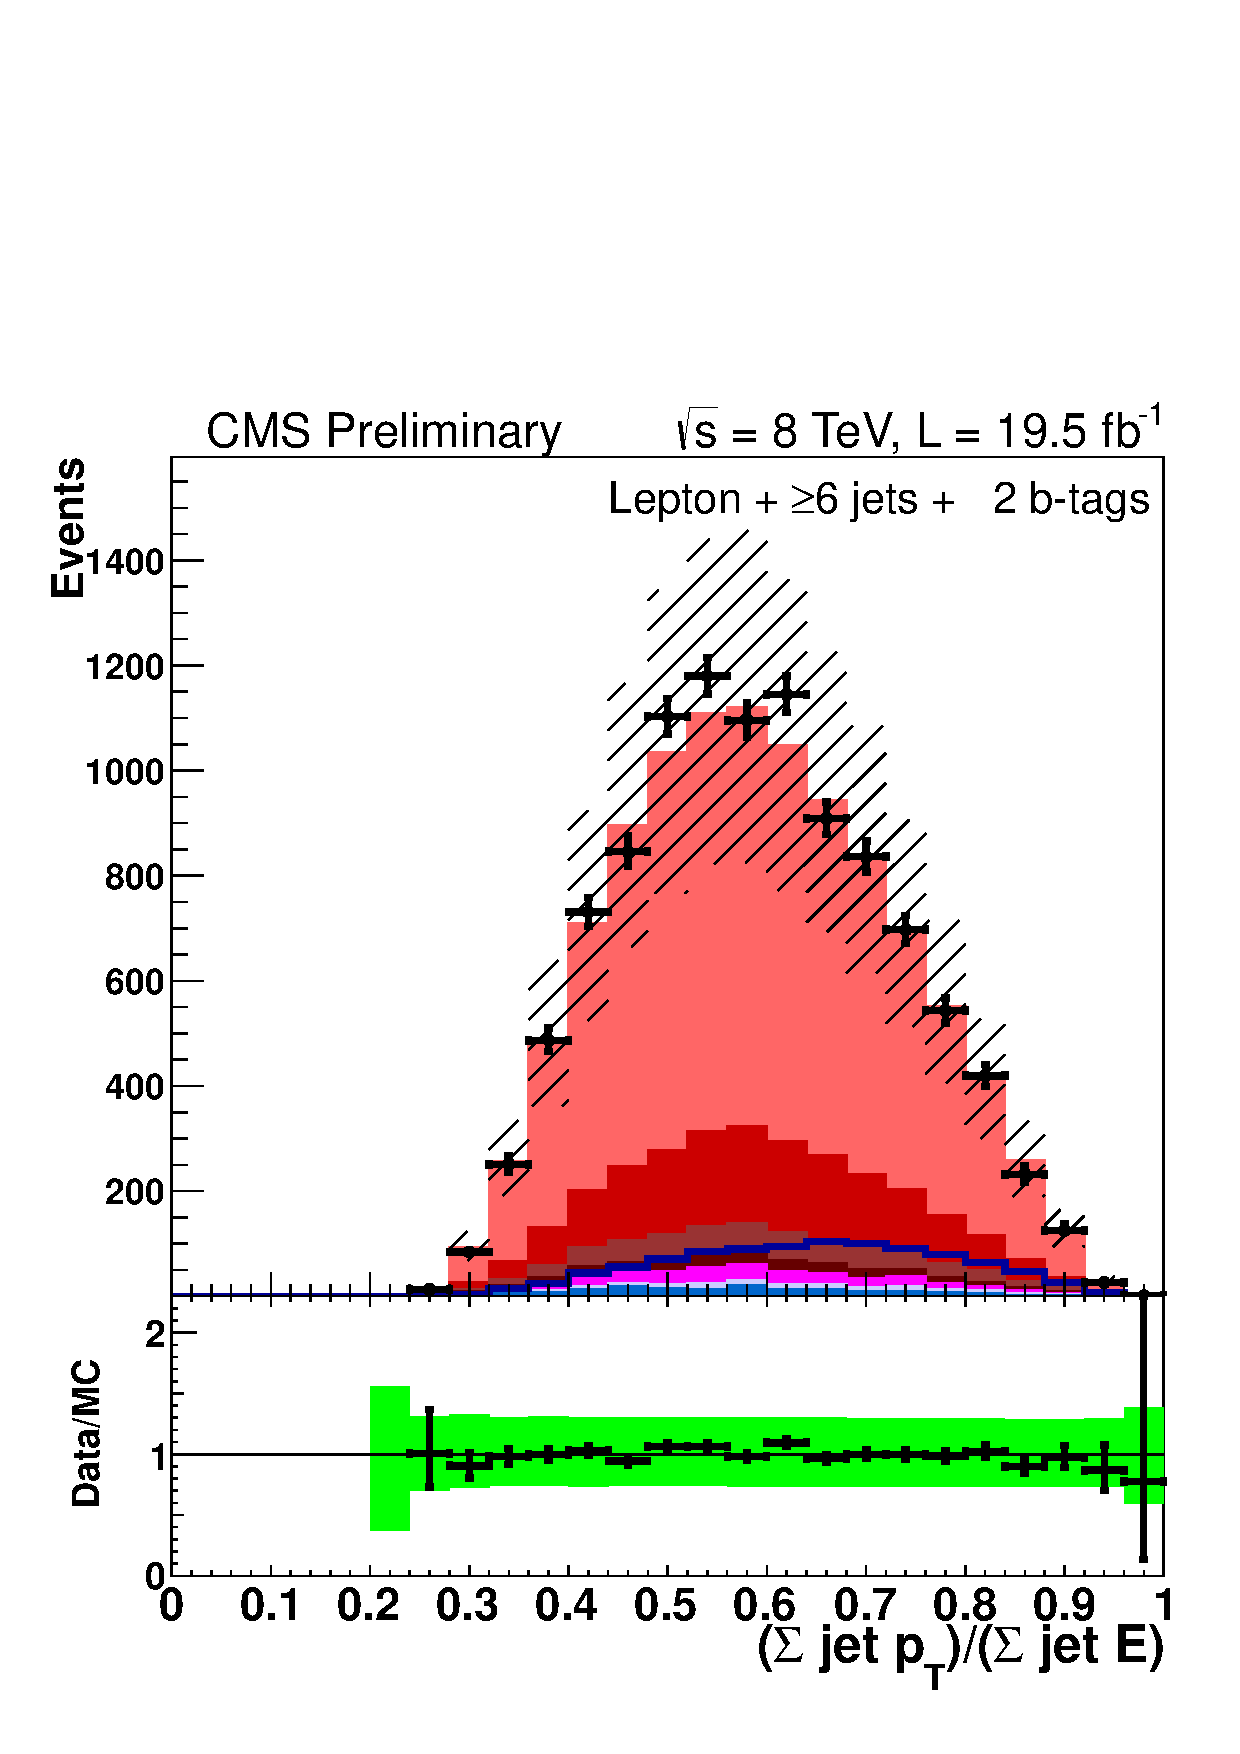
\includegraphics[width=0.31\textwidth]{Figures/Analysis_2_Diagrams/LJ_plots_lep/6j2t/lep_pt_all_jets_over_E_all_jets_6j2t_cumulative_wRatio_noLegend_lin.pdf}
   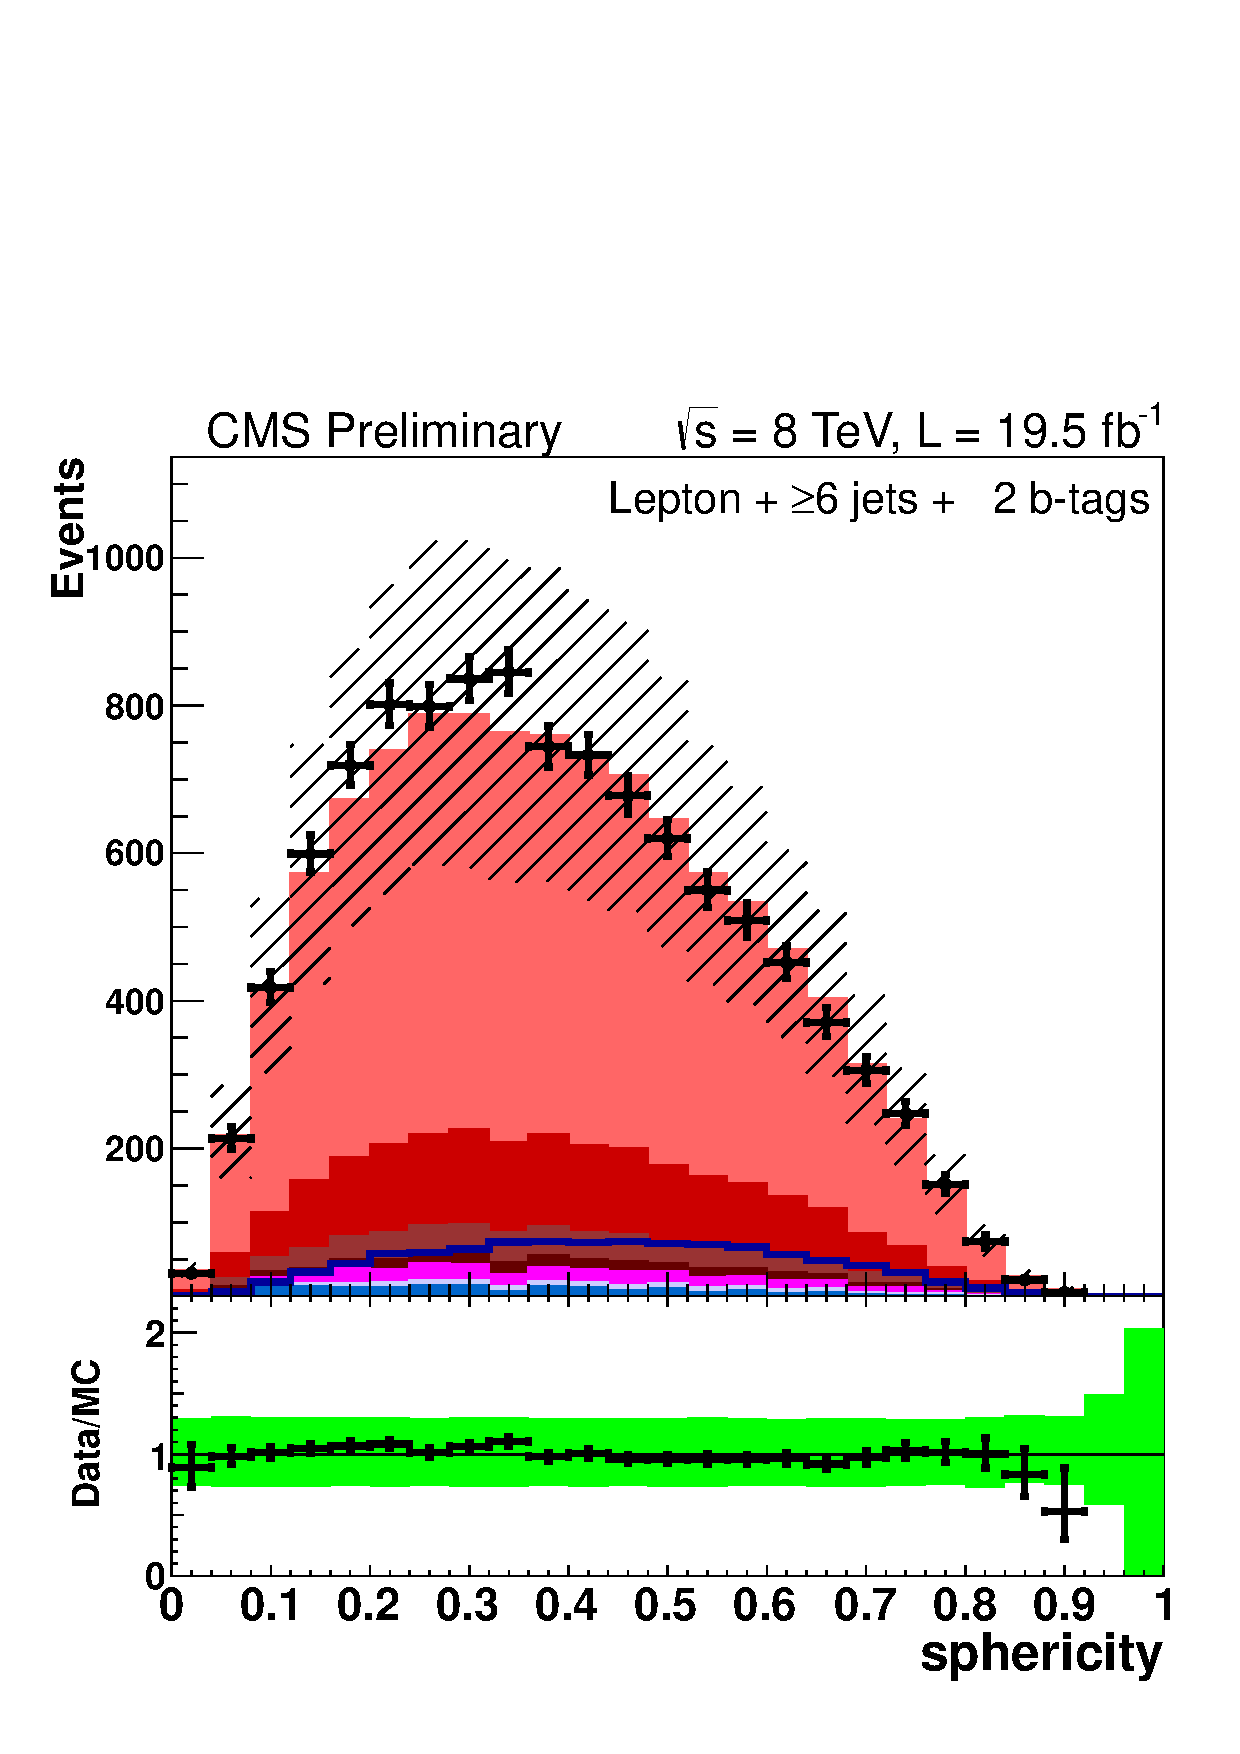
\includegraphics[width=0.31\textwidth]{Figures/Analysis_2_Diagrams/LJ_plots_lep/6j2t/lep_sphericity_6j2t_cumulative_wRatio_noLegend_lin.pdf}
   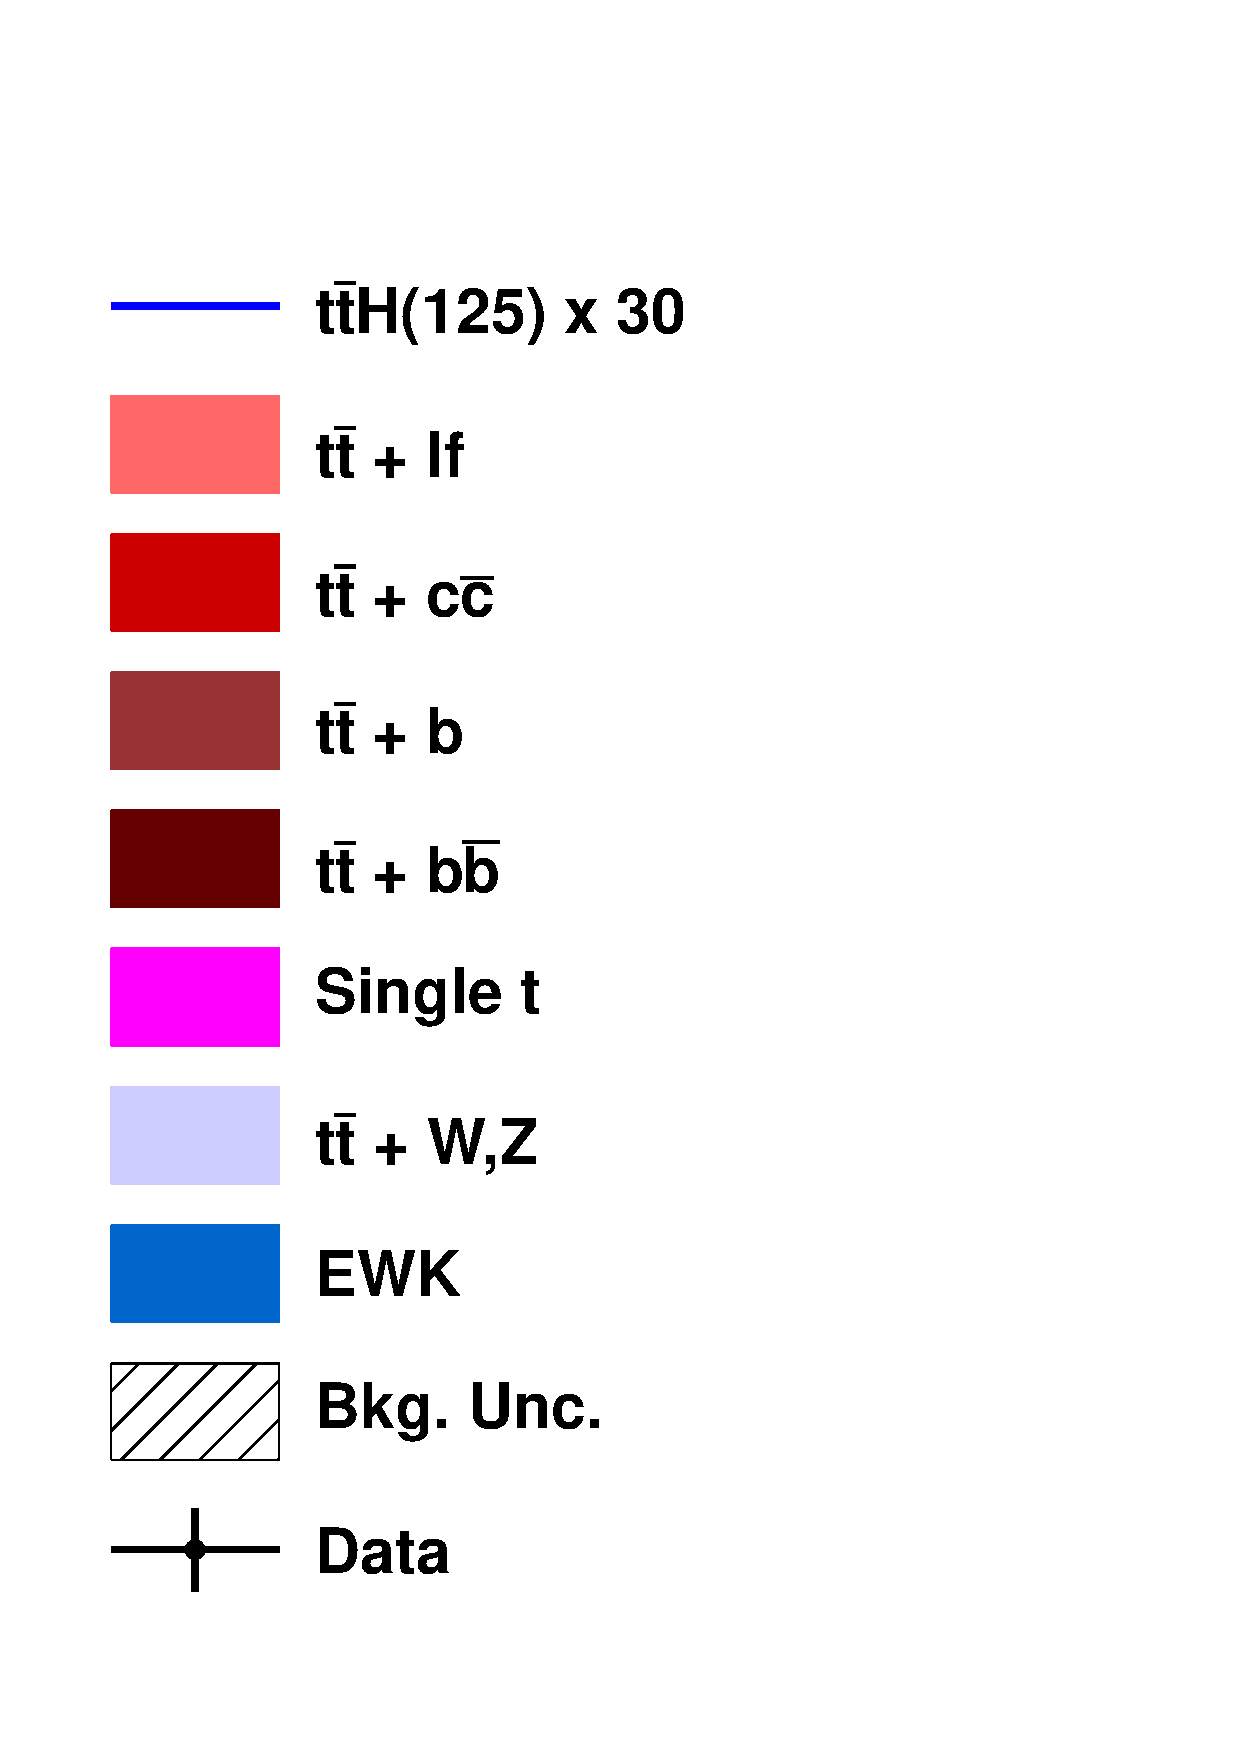
\includegraphics[width=0.15\textwidth]{Figures/Analysis_2_Diagrams/LJ_plots_lep/ttH_legend_1columns.pdf}
   \caption{Data/MC comparisons for events with one lepton and $\ge$6 jets + 2b- tags.  The uncertainty band includes statistical and systematic uncertainties that affect both the rate and shape of the background distributions.}
   \label{fig:lj_input_II_6j2t}
 \end{center}
\end{figure}

\clearpage


\begin{figure}[hbtp]
 \begin{center}
   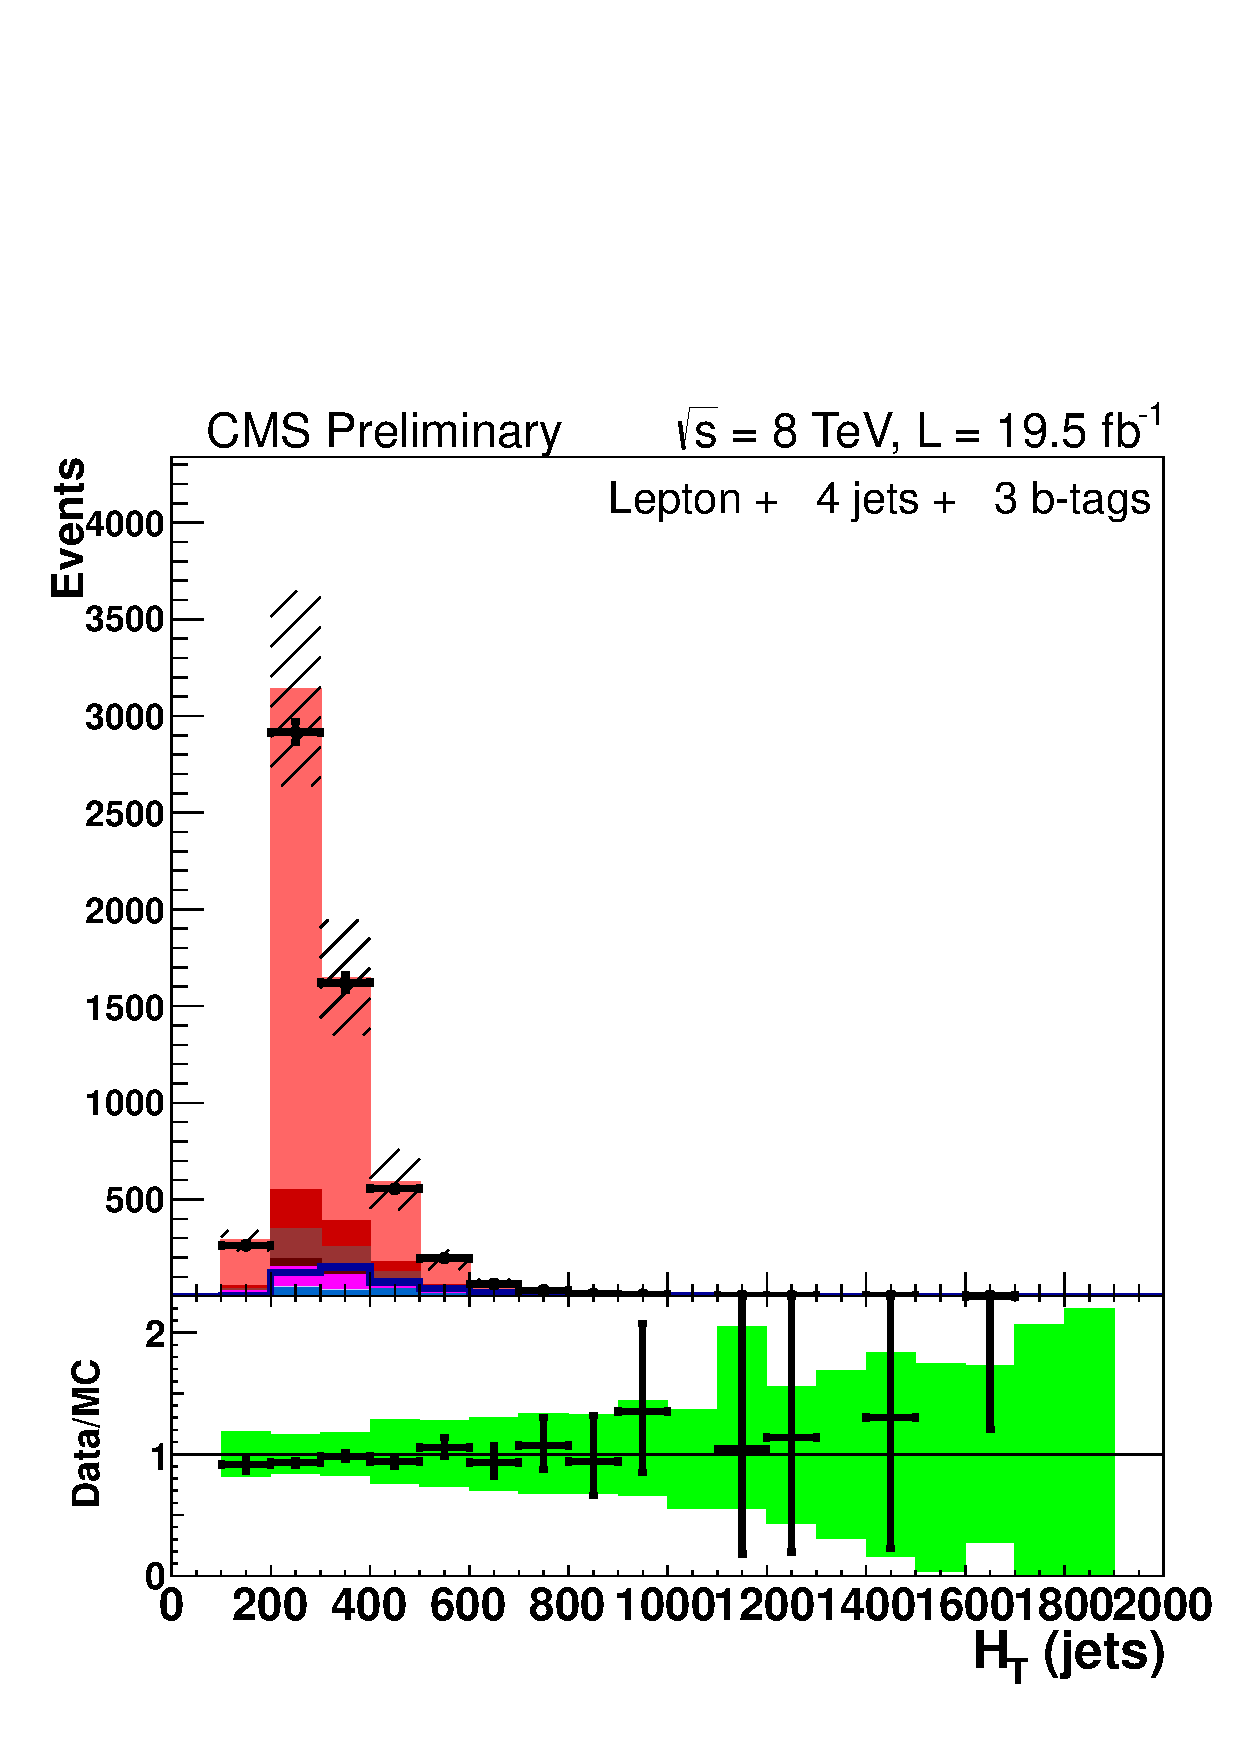
\includegraphics[width=0.31\textwidth]{Figures/Analysis_2_Diagrams/LJ_plots_lep/4j3t/lep_HT_4j3t_cumulative_wRatio_noLegend_lin.pdf}
   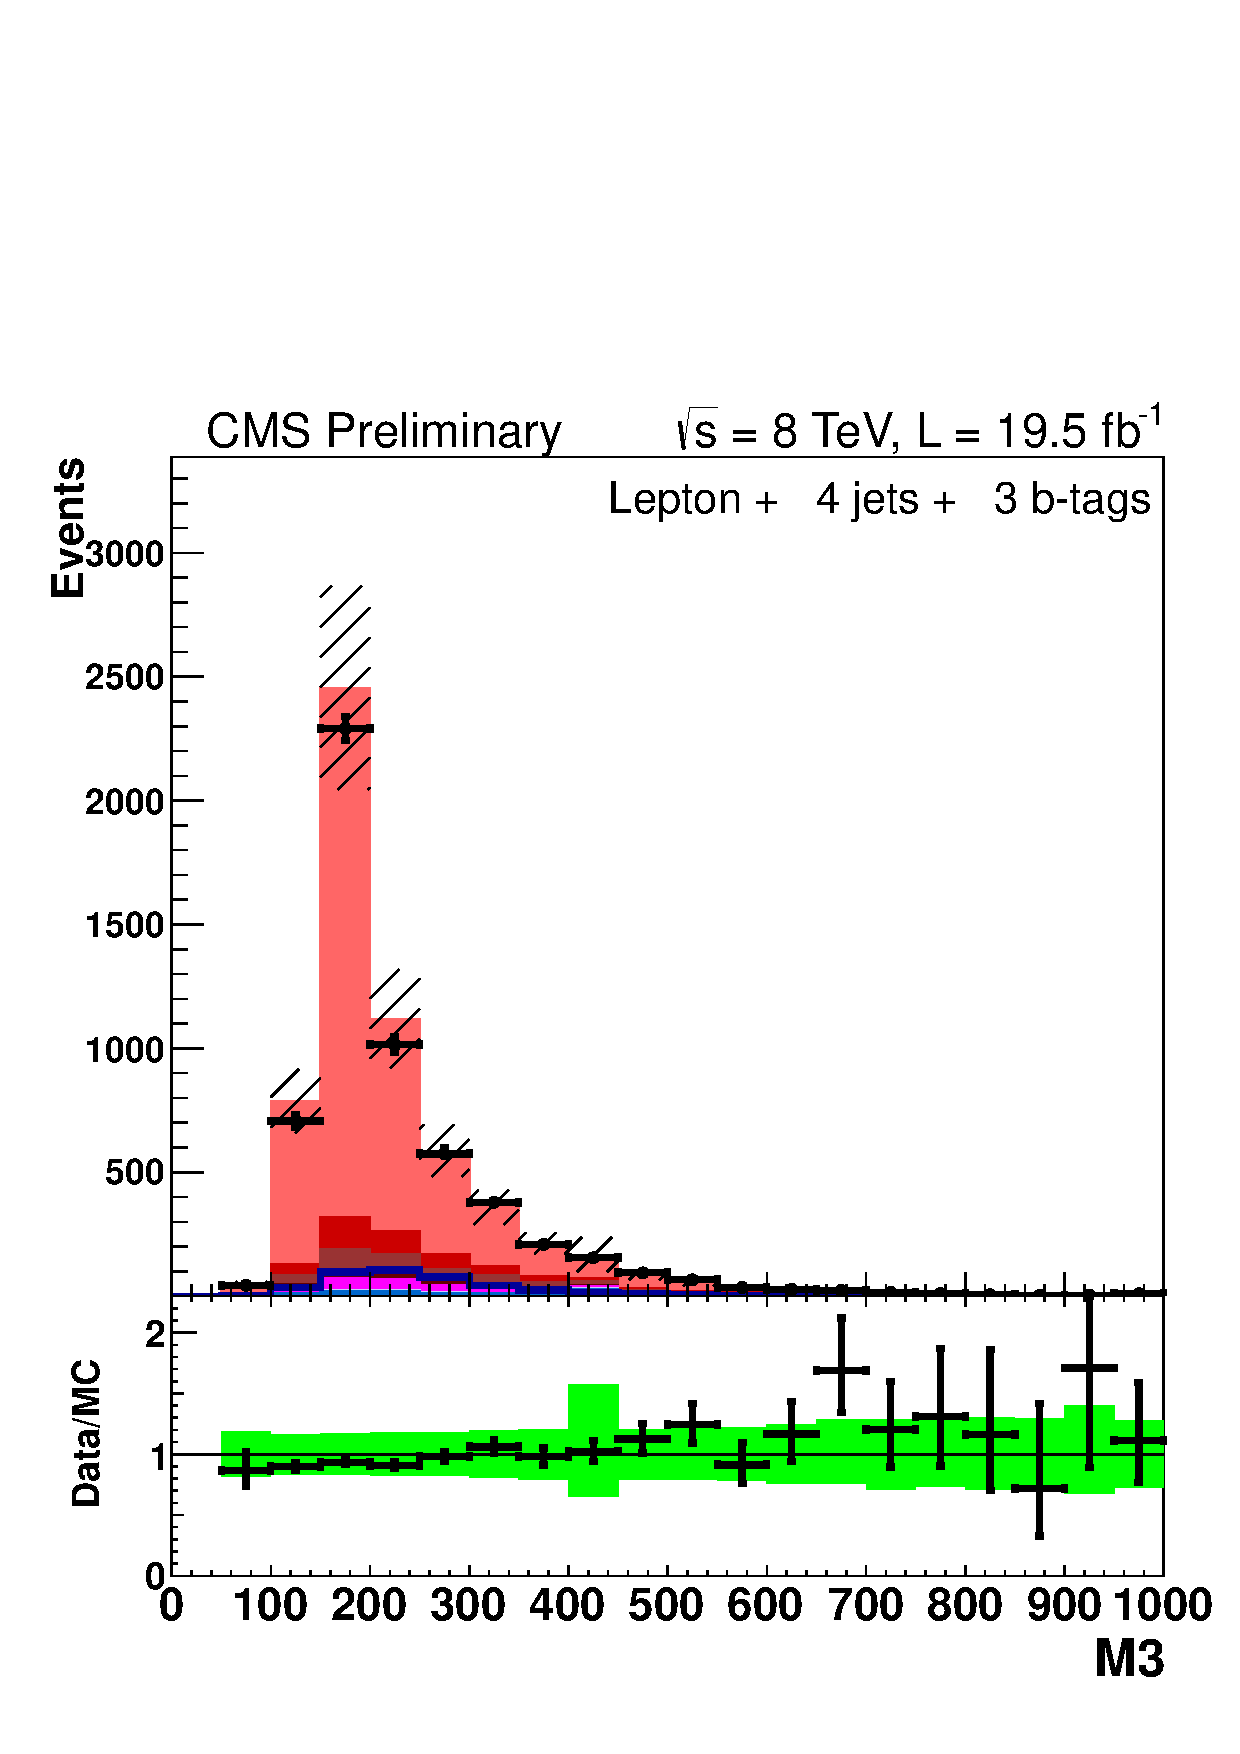
\includegraphics[width=0.31\textwidth]{Figures/Analysis_2_Diagrams/LJ_plots_lep/4j3t/lep_M3_4j3t_cumulative_wRatio_noLegend_lin.pdf}
   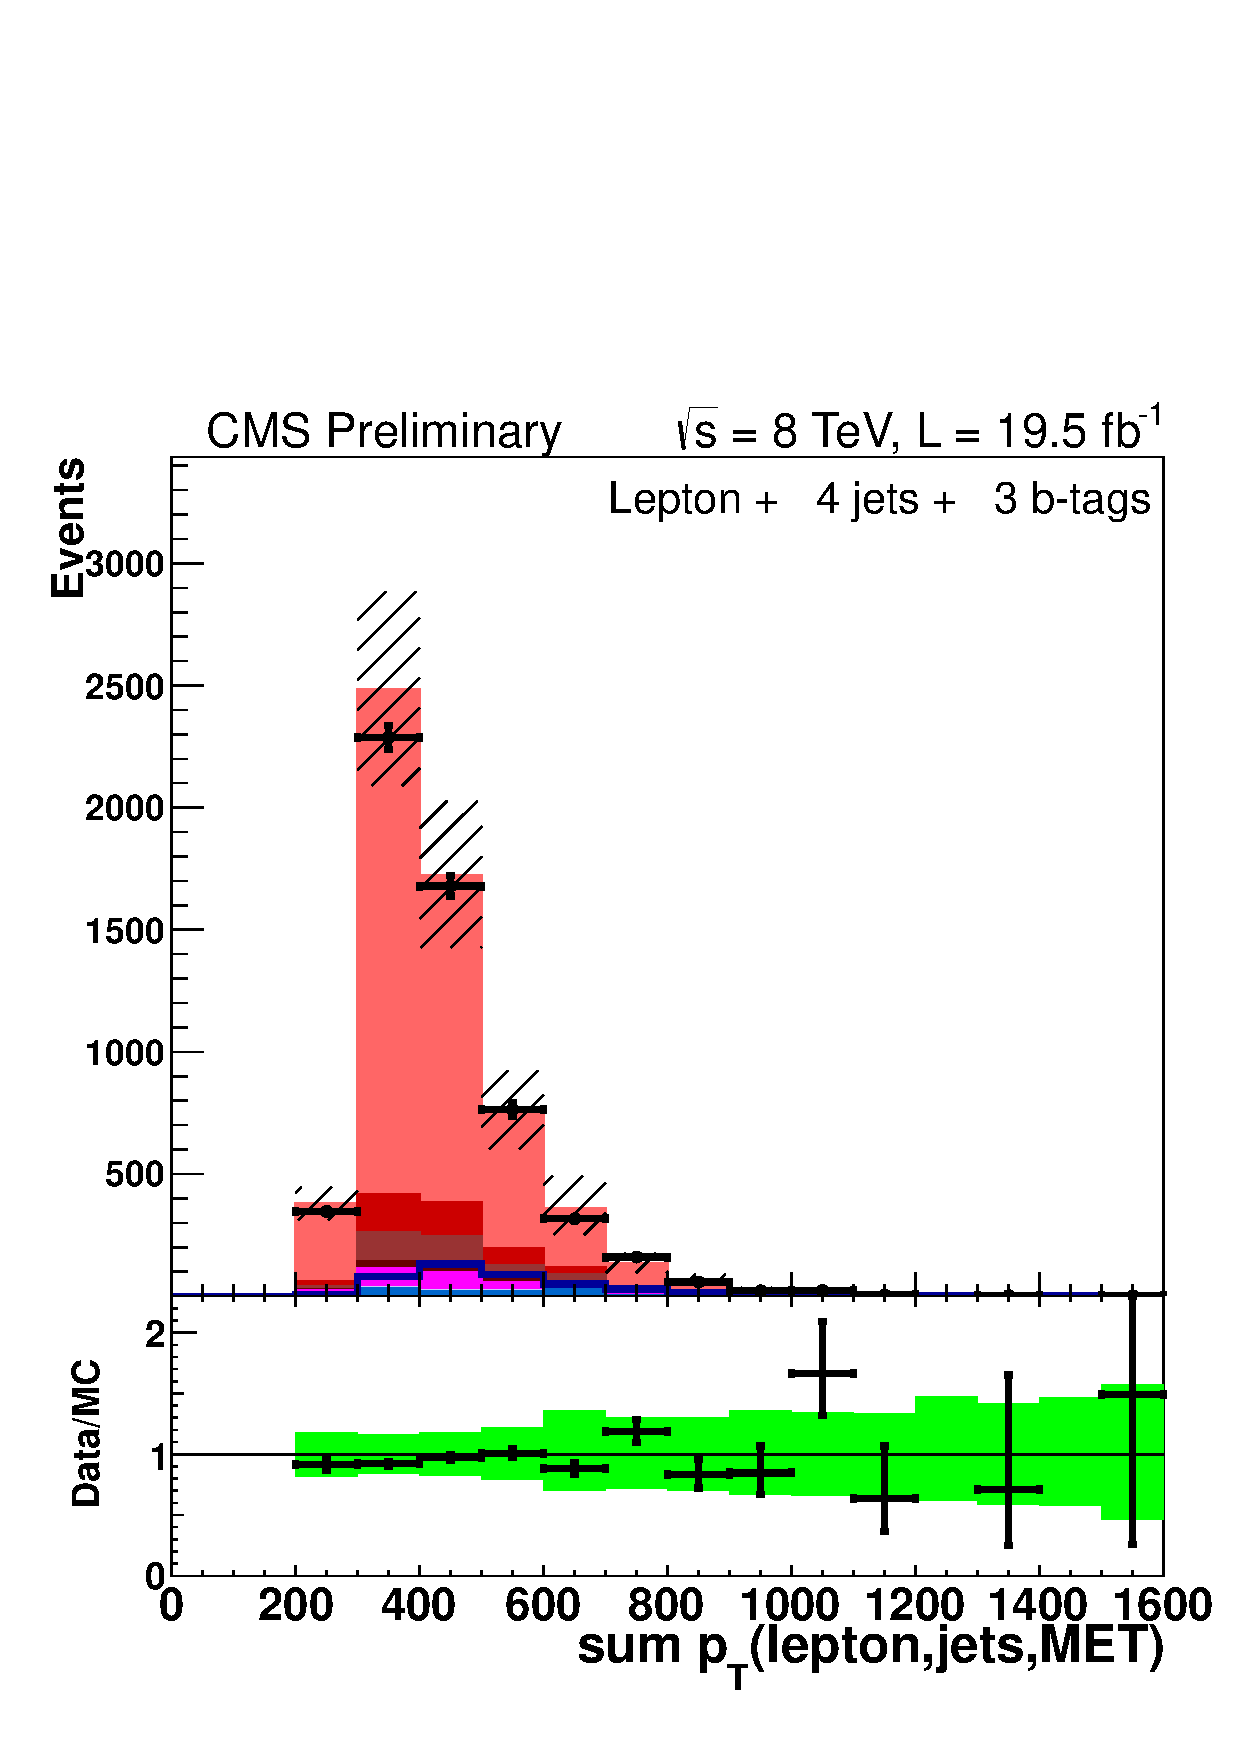
\includegraphics[width=0.31\textwidth]{Figures/Analysis_2_Diagrams/LJ_plots_lep/4j3t/lep_all_sum_pt_with_met_4j3t_cumulative_wRatio_noLegend_lin.pdf}
   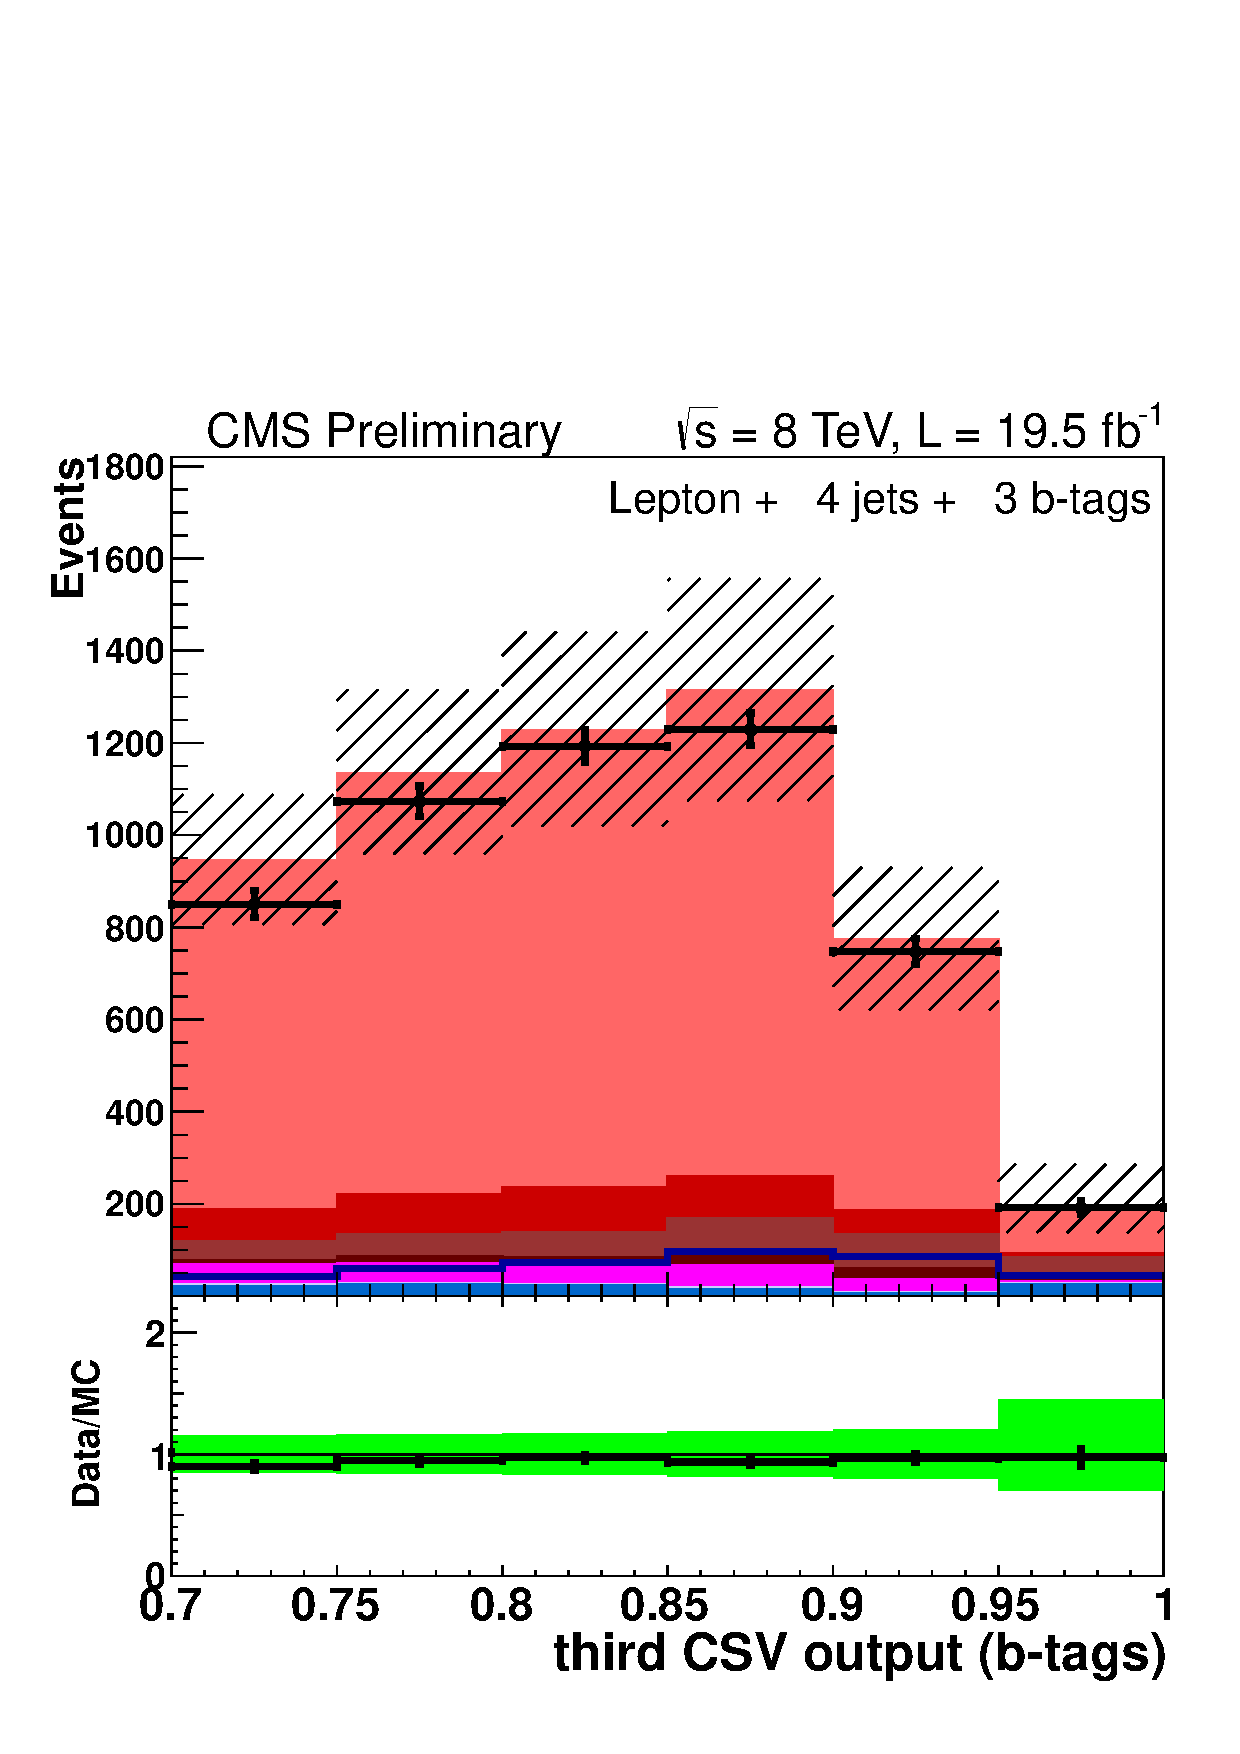
\includegraphics[width=0.31\textwidth]{Figures/Analysis_2_Diagrams/LJ_plots_lep/4j3t/lep_jet_csv_3_4j3t_cumulative_wRatio_noLegend_lin.pdf}
   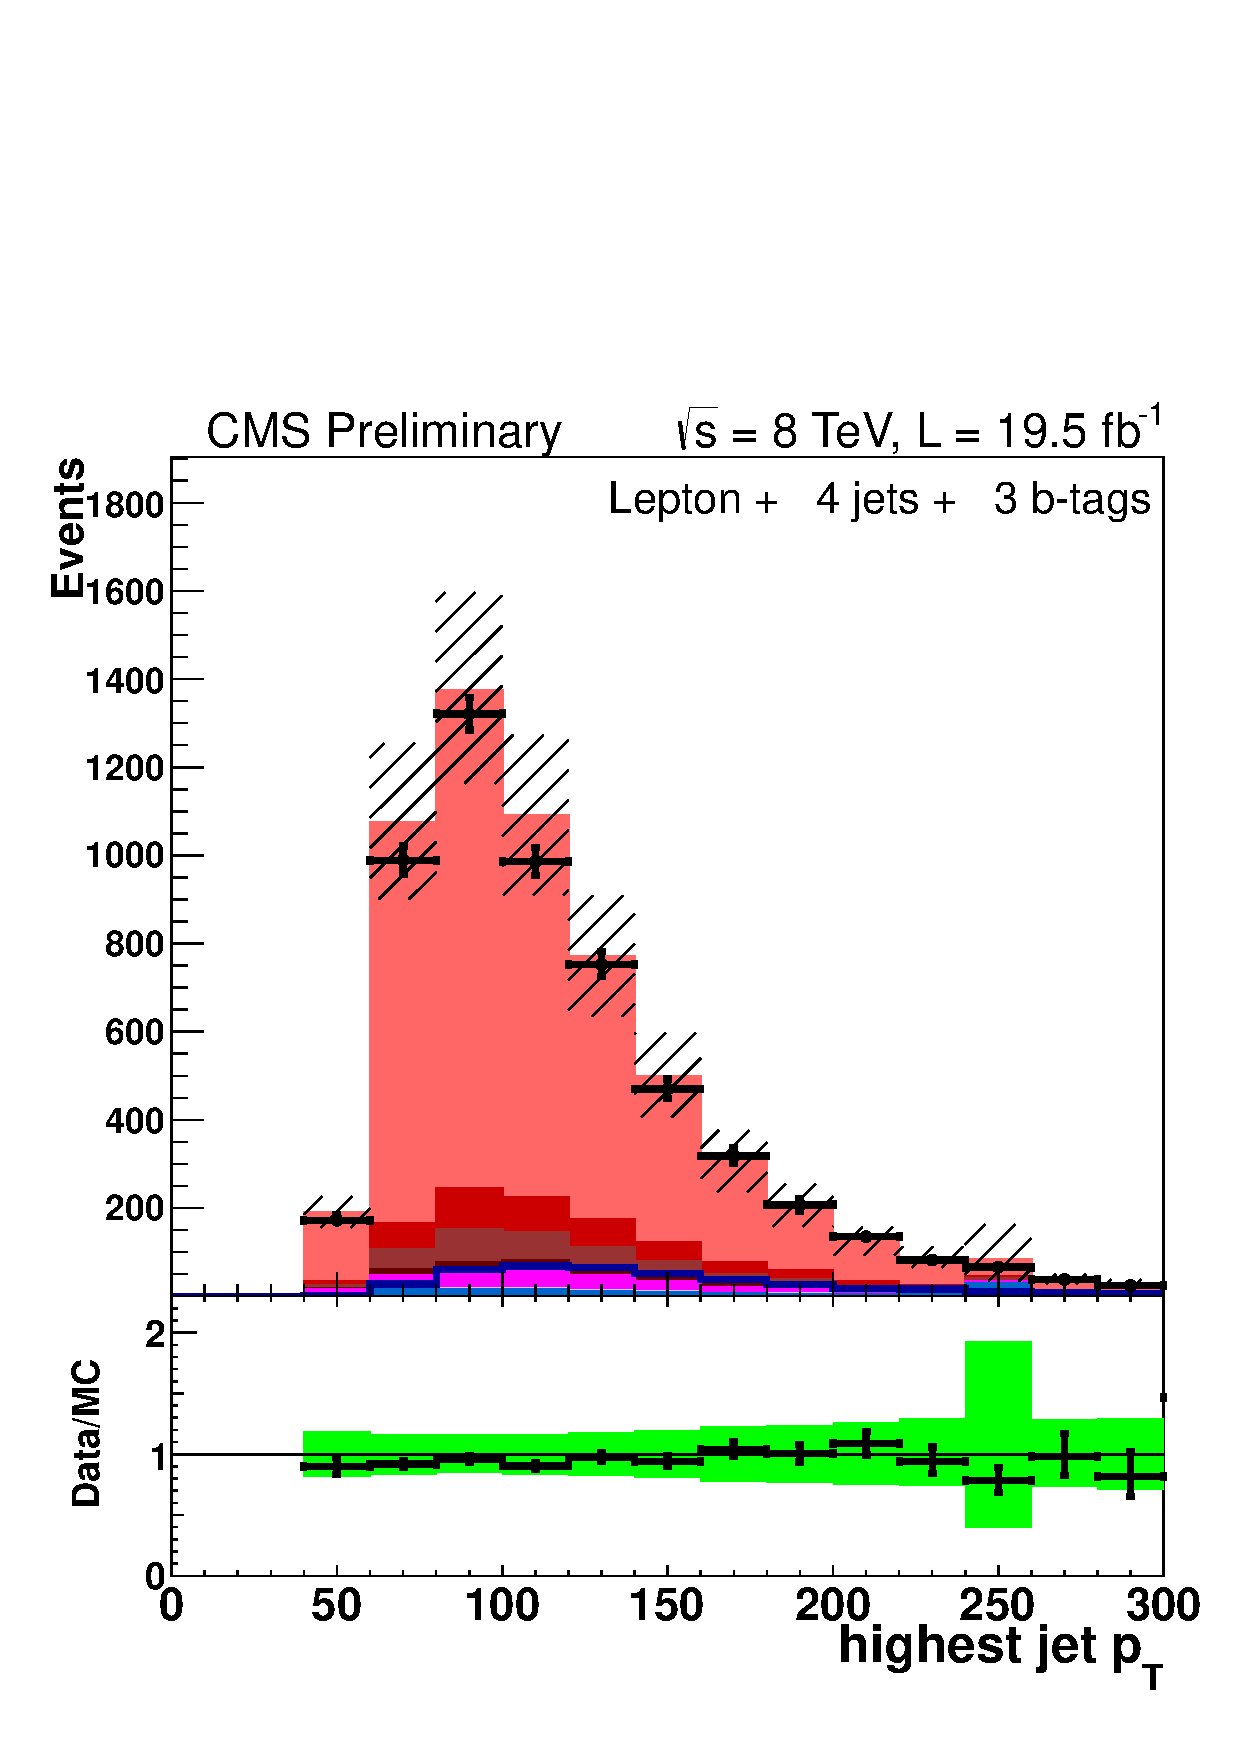
\includegraphics[width=0.31\textwidth]{Figures/Analysis_2_Diagrams/LJ_plots_lep/4j3t/lep_jet_pt_1_4j3t_cumulative_wRatio_noLegend_lin.pdf}
   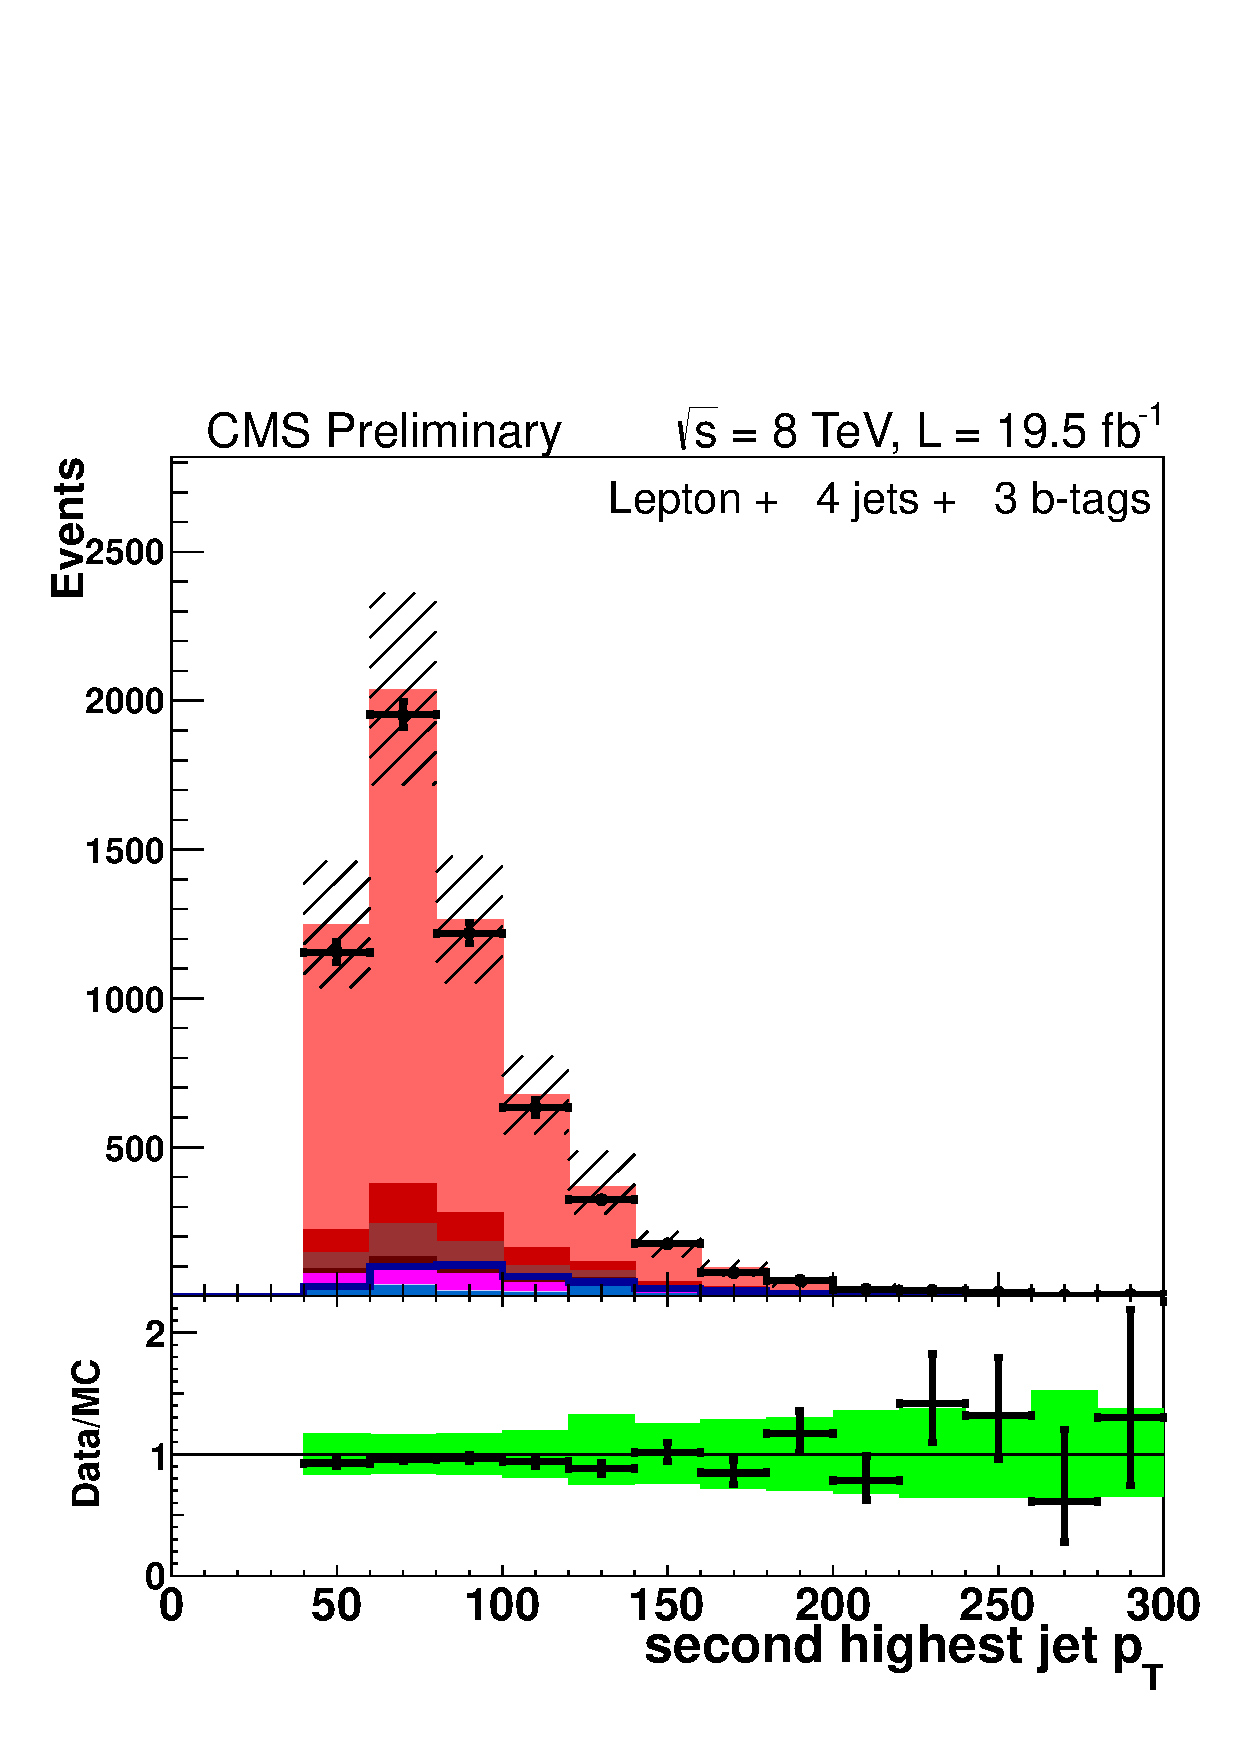
\includegraphics[width=0.31\textwidth]{Figures/Analysis_2_Diagrams/LJ_plots_lep/4j3t/lep_jet_pt_2_4j3t_cumulative_wRatio_noLegend_lin.pdf}
   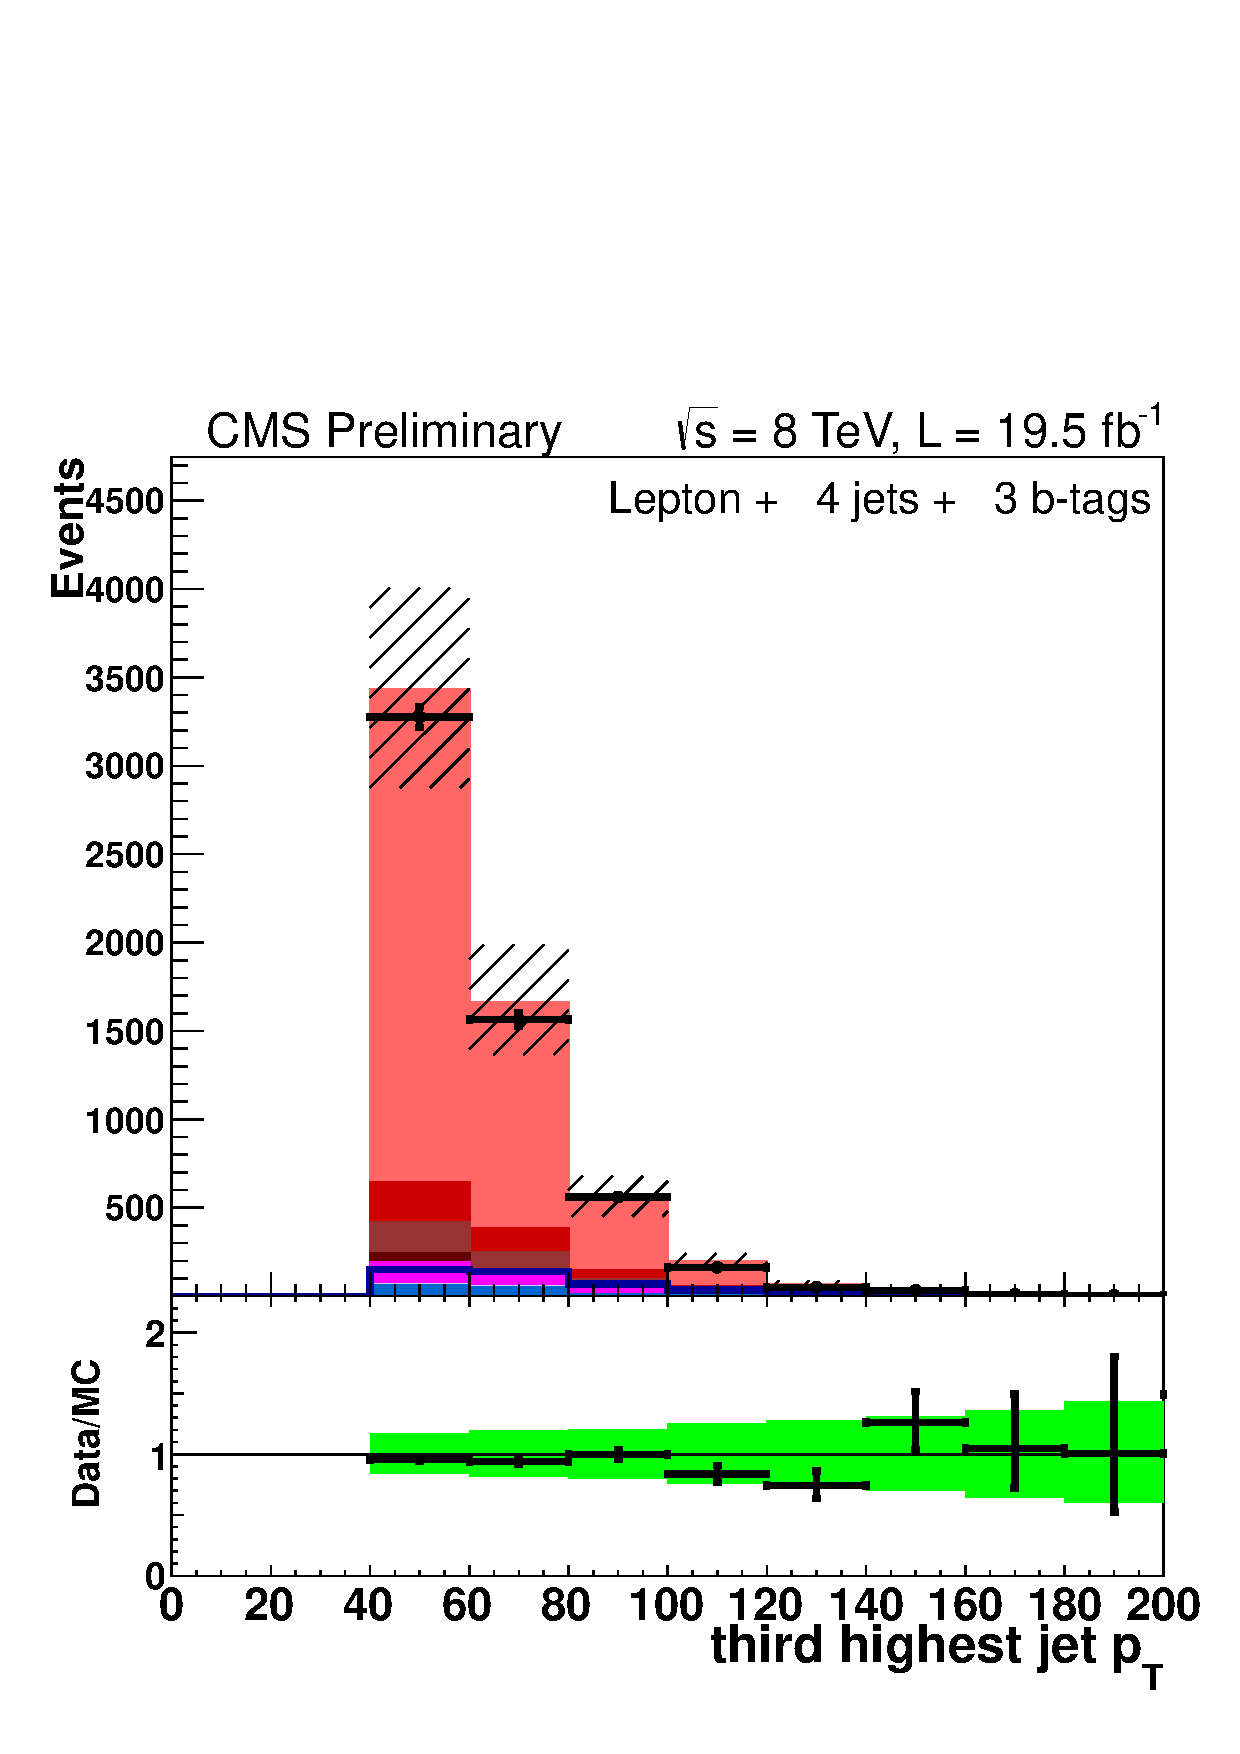
\includegraphics[width=0.31\textwidth]{Figures/Analysis_2_Diagrams/LJ_plots_lep/4j3t/lep_jet_pt_3_4j3t_cumulative_wRatio_noLegend_lin.pdf}
   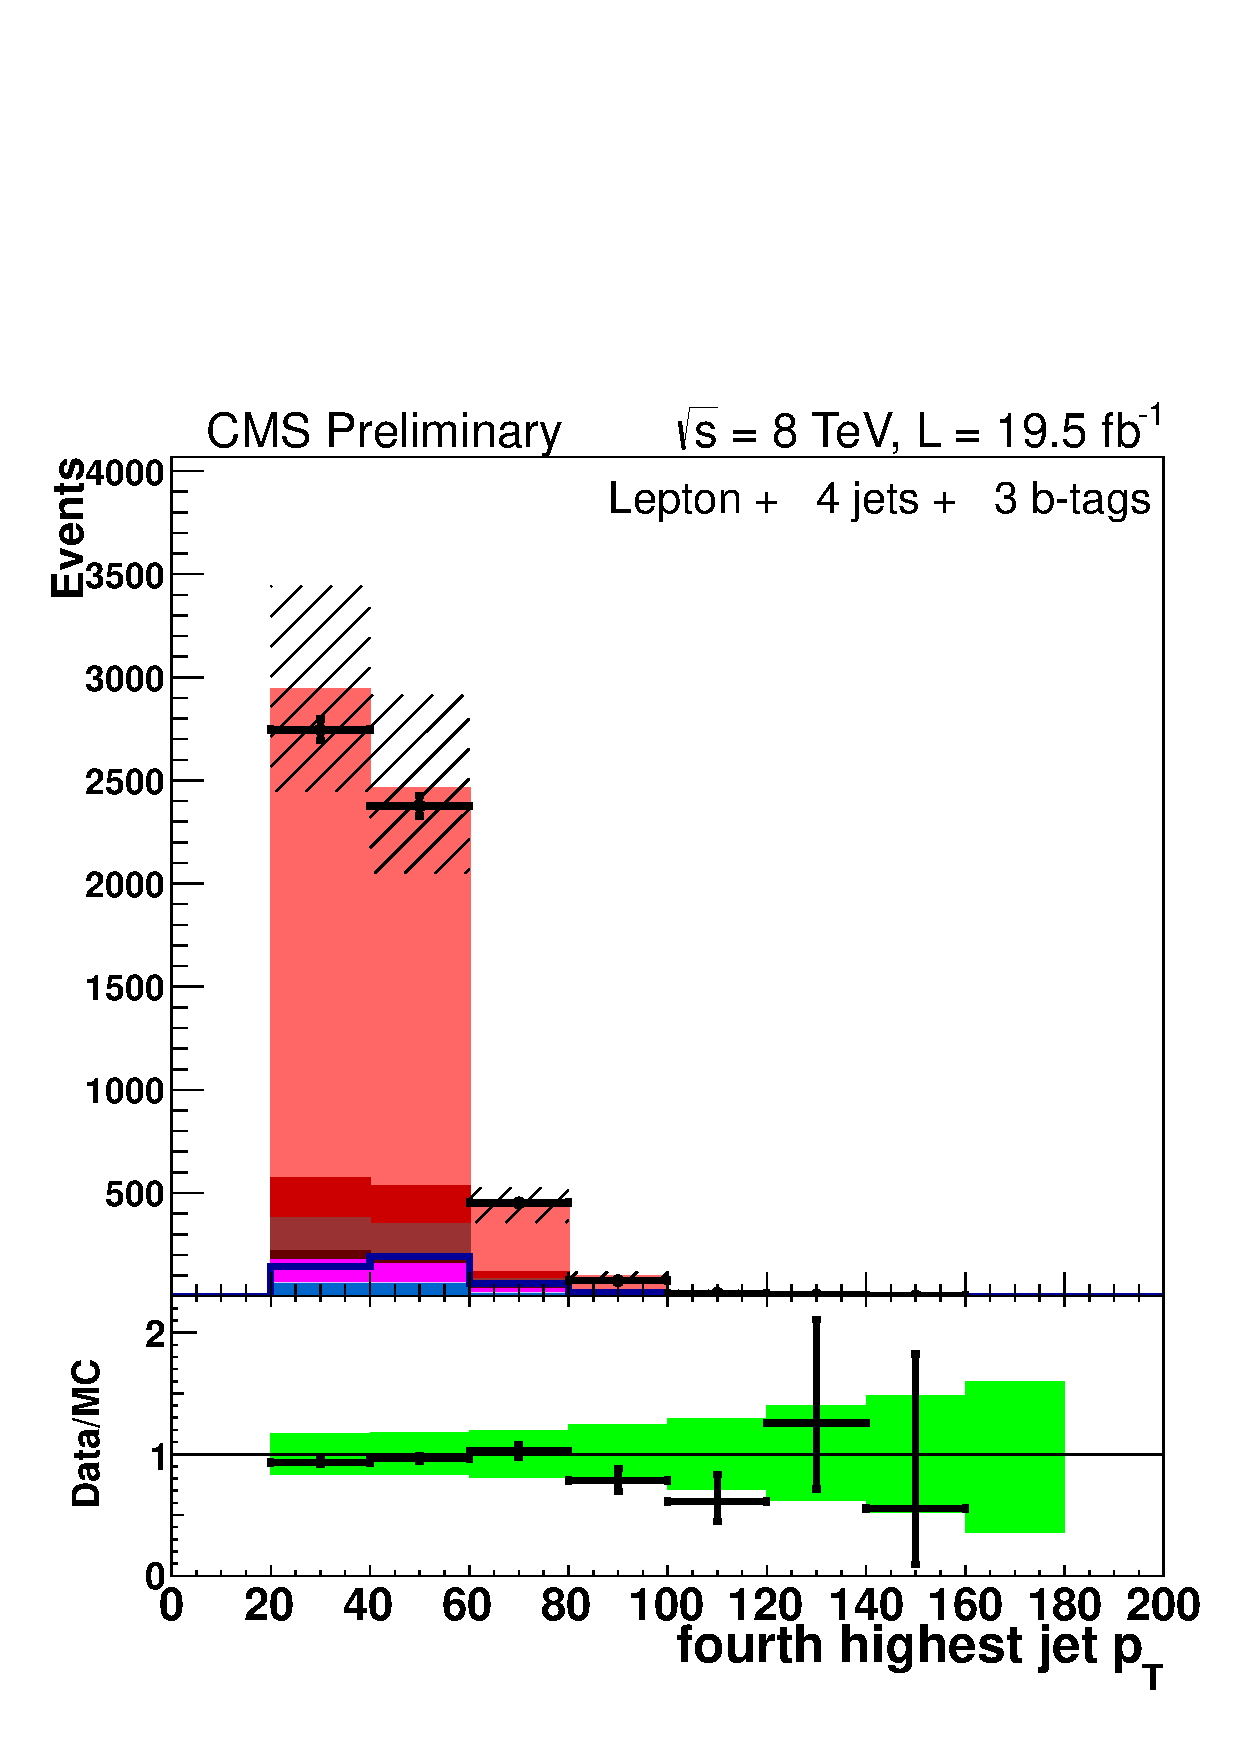
\includegraphics[width=0.31\textwidth]{Figures/Analysis_2_Diagrams/LJ_plots_lep/4j3t/lep_jet_pt_4_4j3t_cumulative_wRatio_noLegend_lin.pdf}
   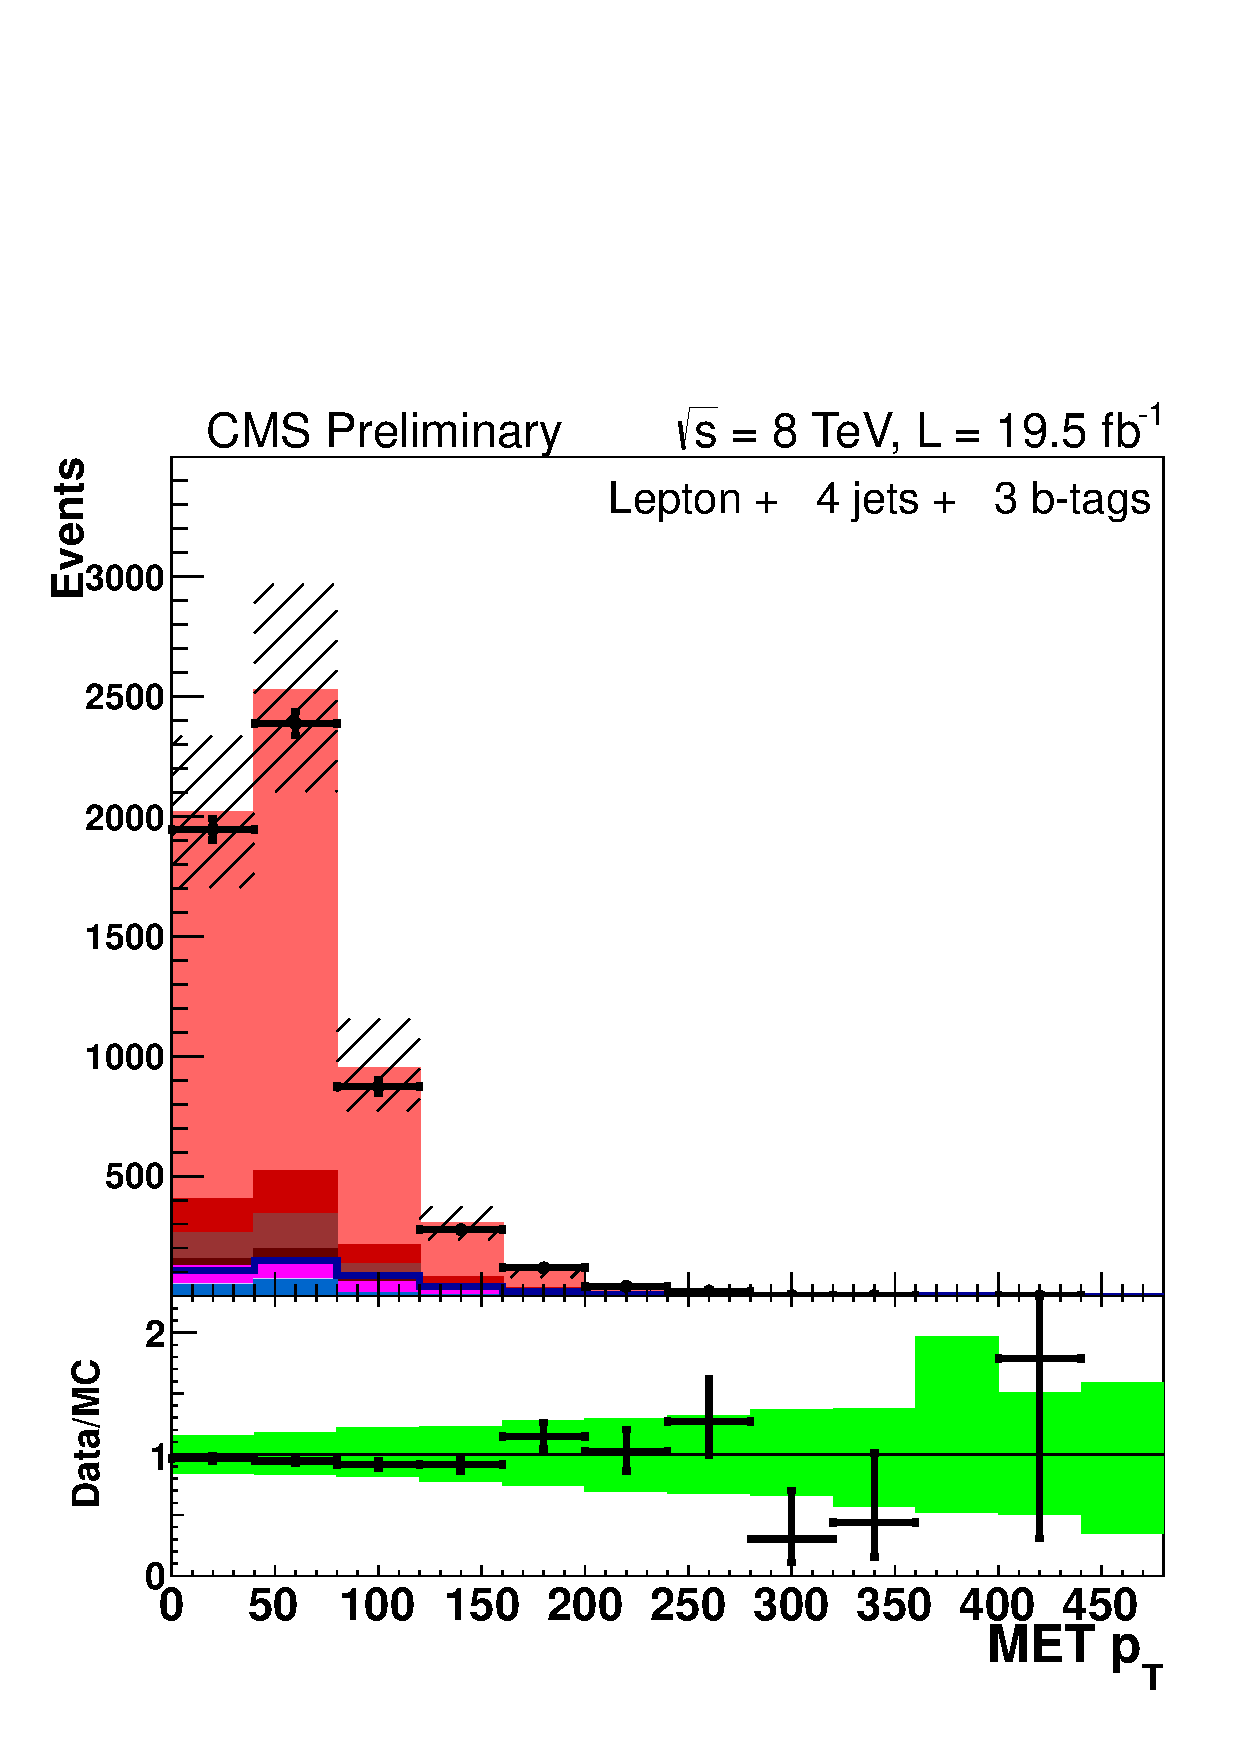
\includegraphics[width=0.31\textwidth]{Figures/Analysis_2_Diagrams/LJ_plots_lep/4j3t/lep_met_pt_4j3t_cumulative_wRatio_noLegend_lin.pdf}
   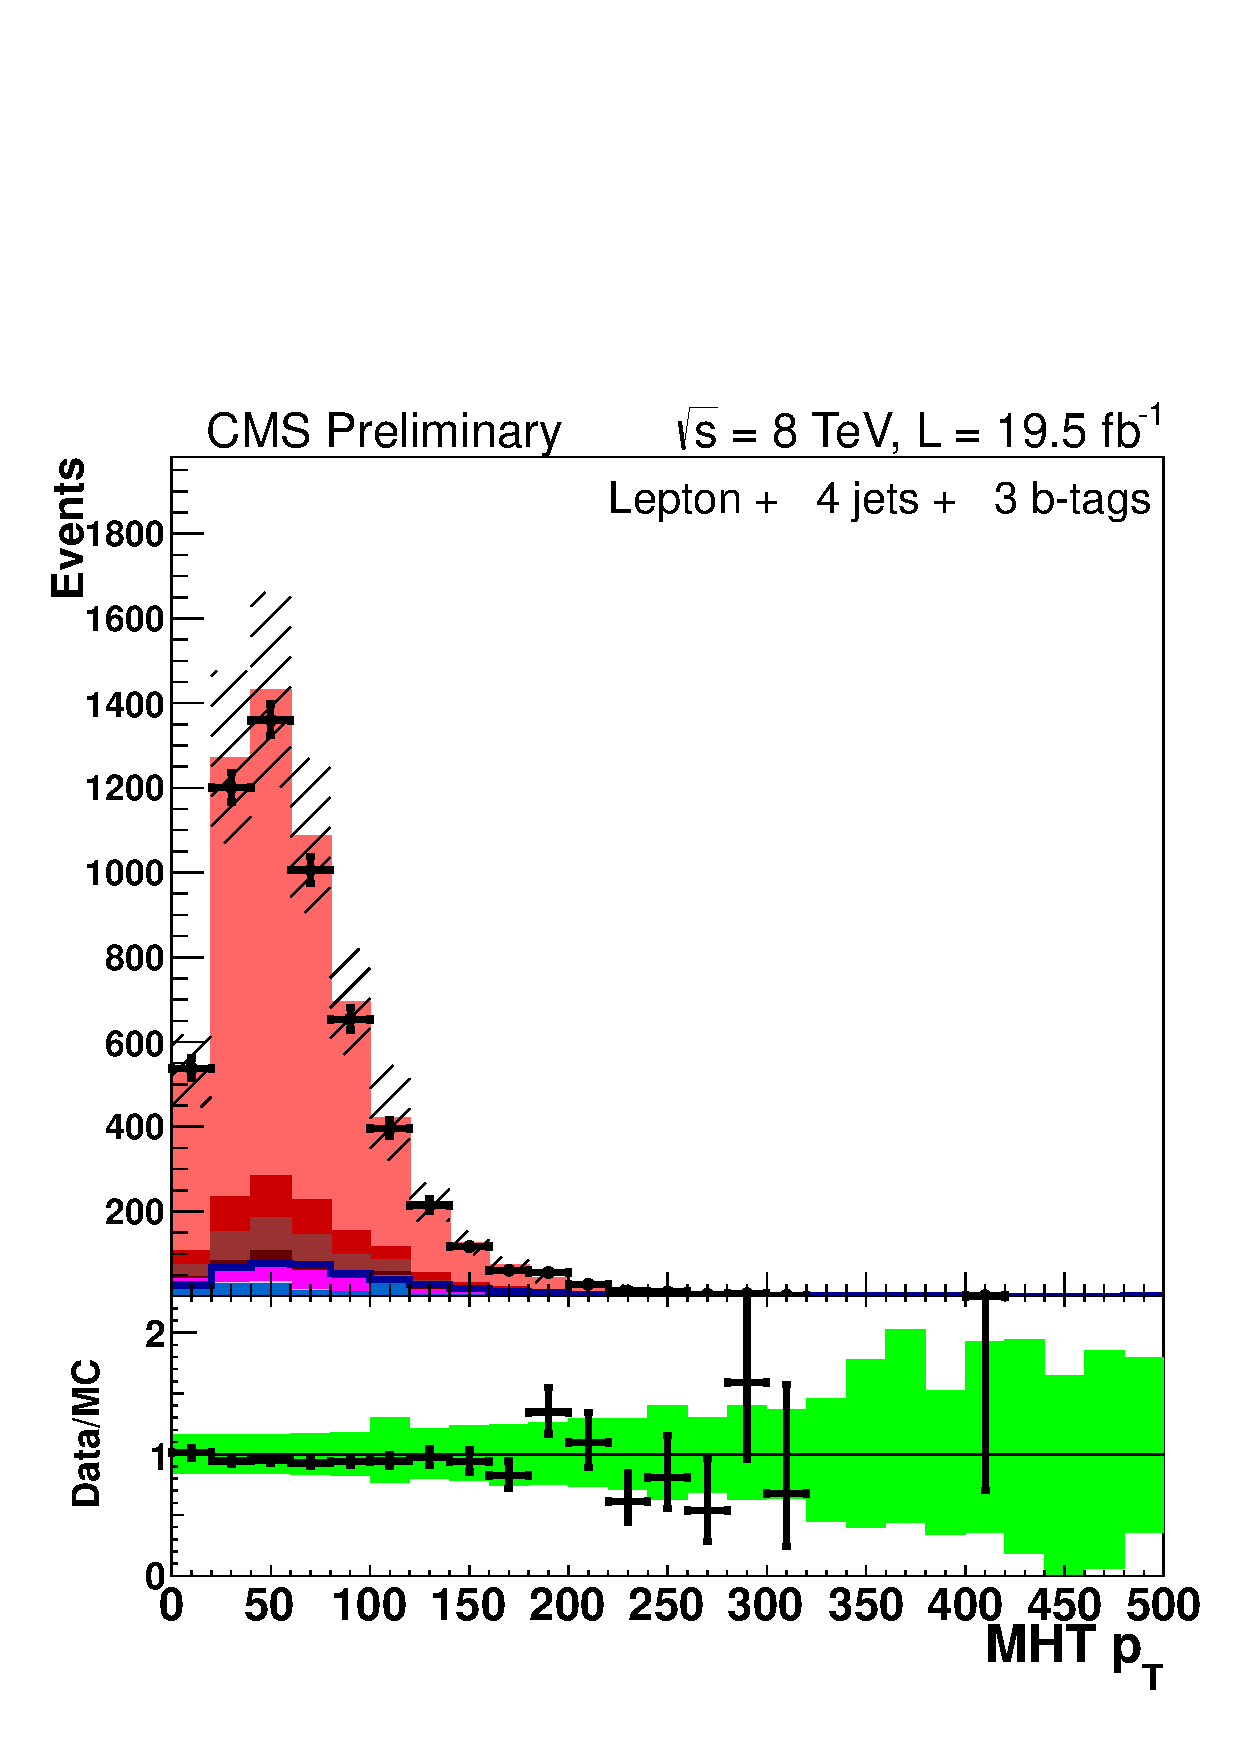
\includegraphics[width=0.31\textwidth]{Figures/Analysis_2_Diagrams/LJ_plots_lep/4j3t/lep_mht_pt_4j3t_cumulative_wRatio_noLegend_lin.pdf}
   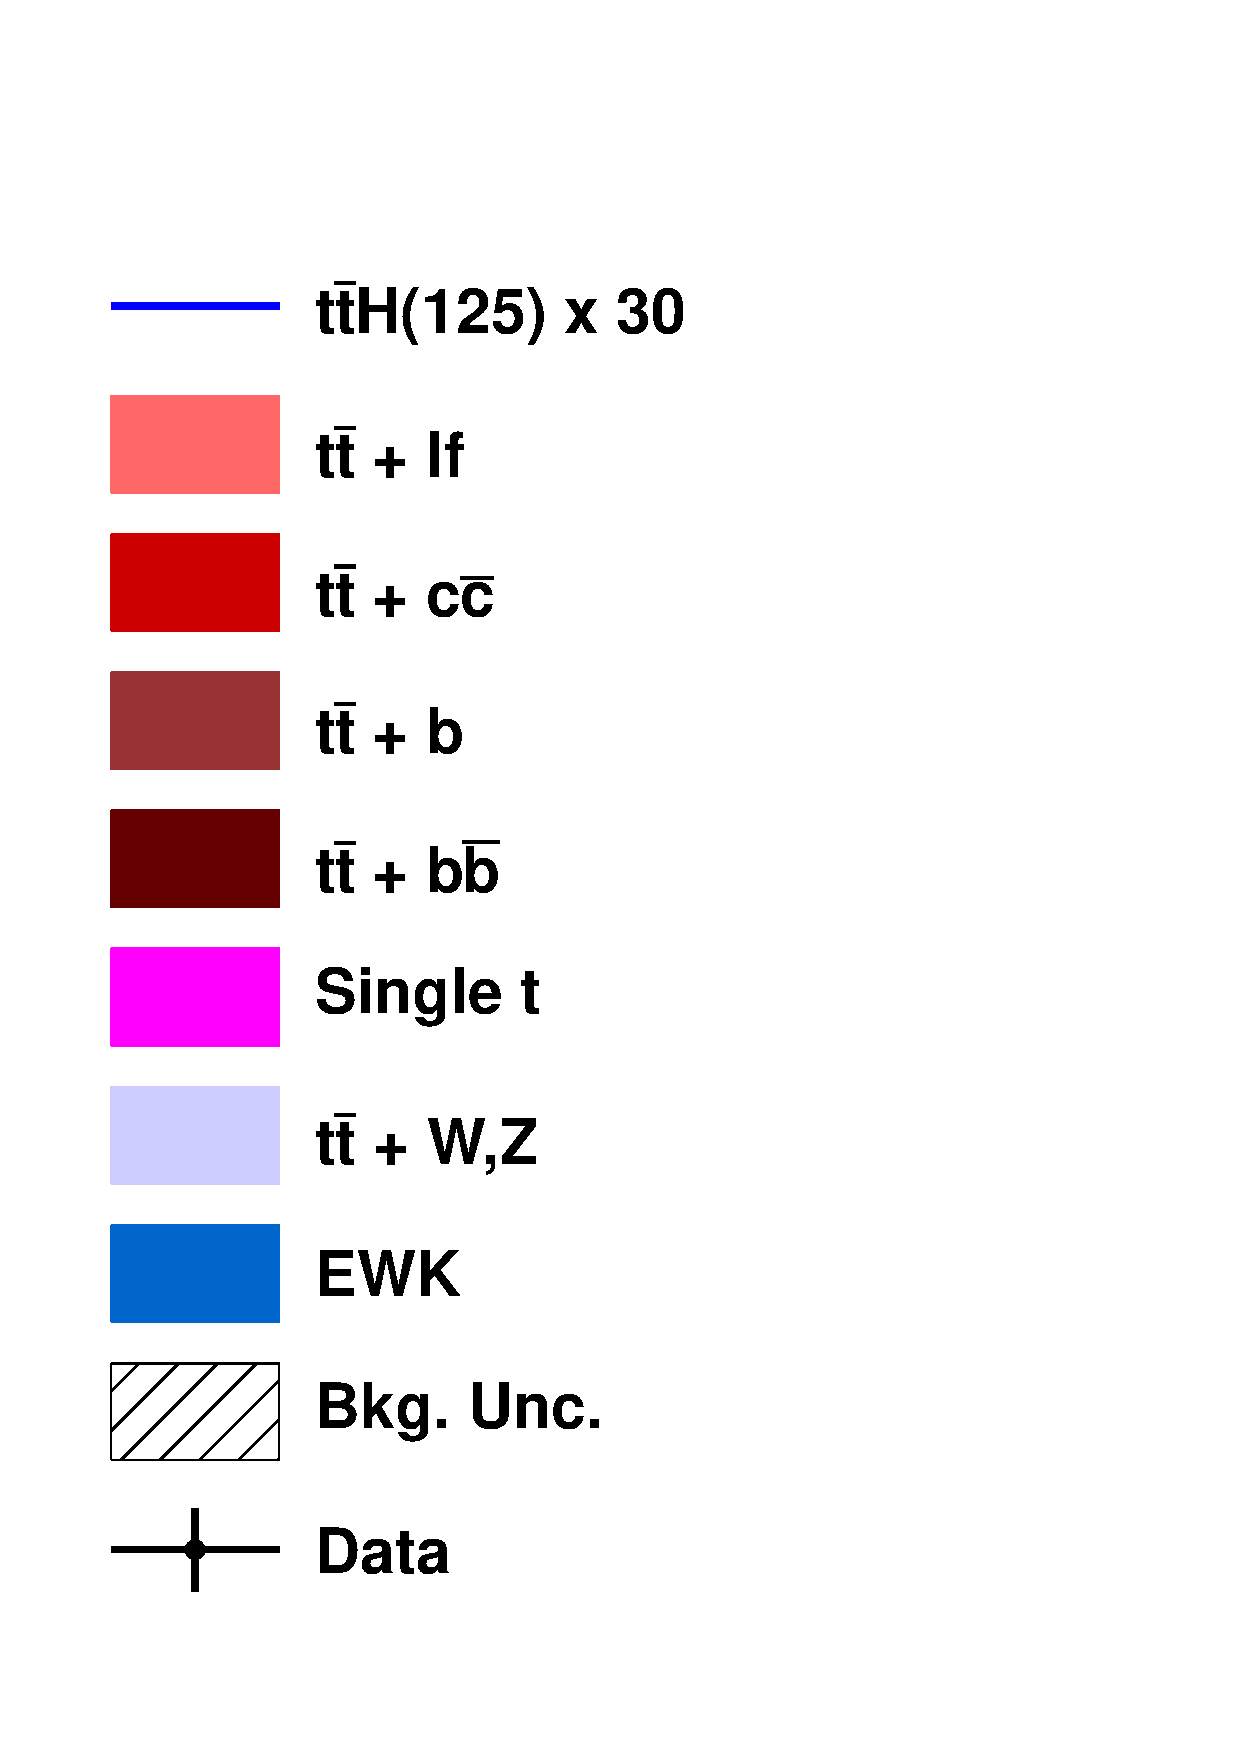
\includegraphics[width=0.15\textwidth]{Figures/Analysis_2_Diagrams/LJ_plots_lep/ttH_legend_1columns.pdf}
   \caption{Data/MC comparisons for events with one lepton and 4 jets + 3 b-tags.  The uncertainty band includes statistical and systematic uncertainties that affect both the rate and shape of the background distributions.}
   \label{fig:lj_input_II_4j3t}
 \end{center}
\end{figure}

\clearpage


\begin{figure}[hbtp]
 \begin{center}
   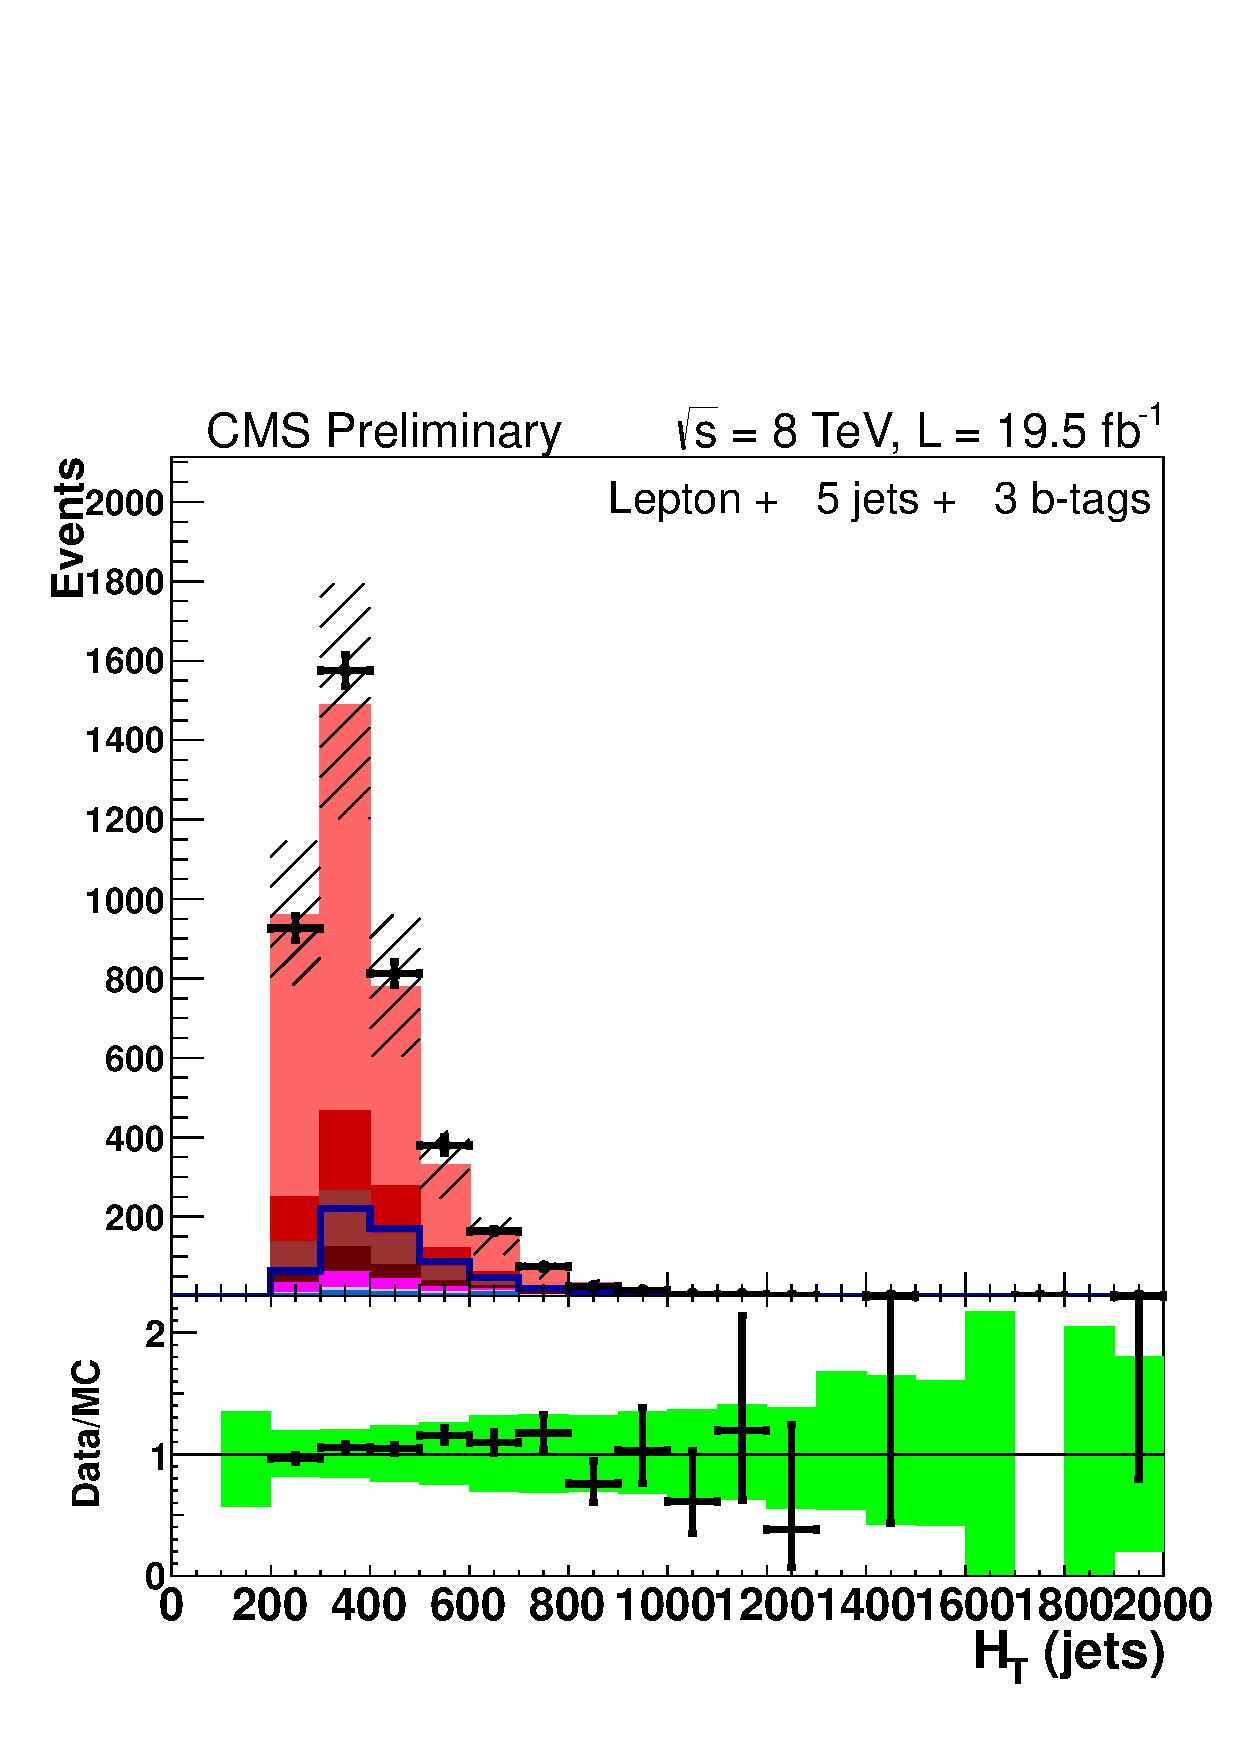
\includegraphics[width=0.31\textwidth]{Figures/Analysis_2_Diagrams/LJ_plots_lep/5j3t/lep_HT_5j3t_cumulative_wRatio_noLegend_lin.pdf}
   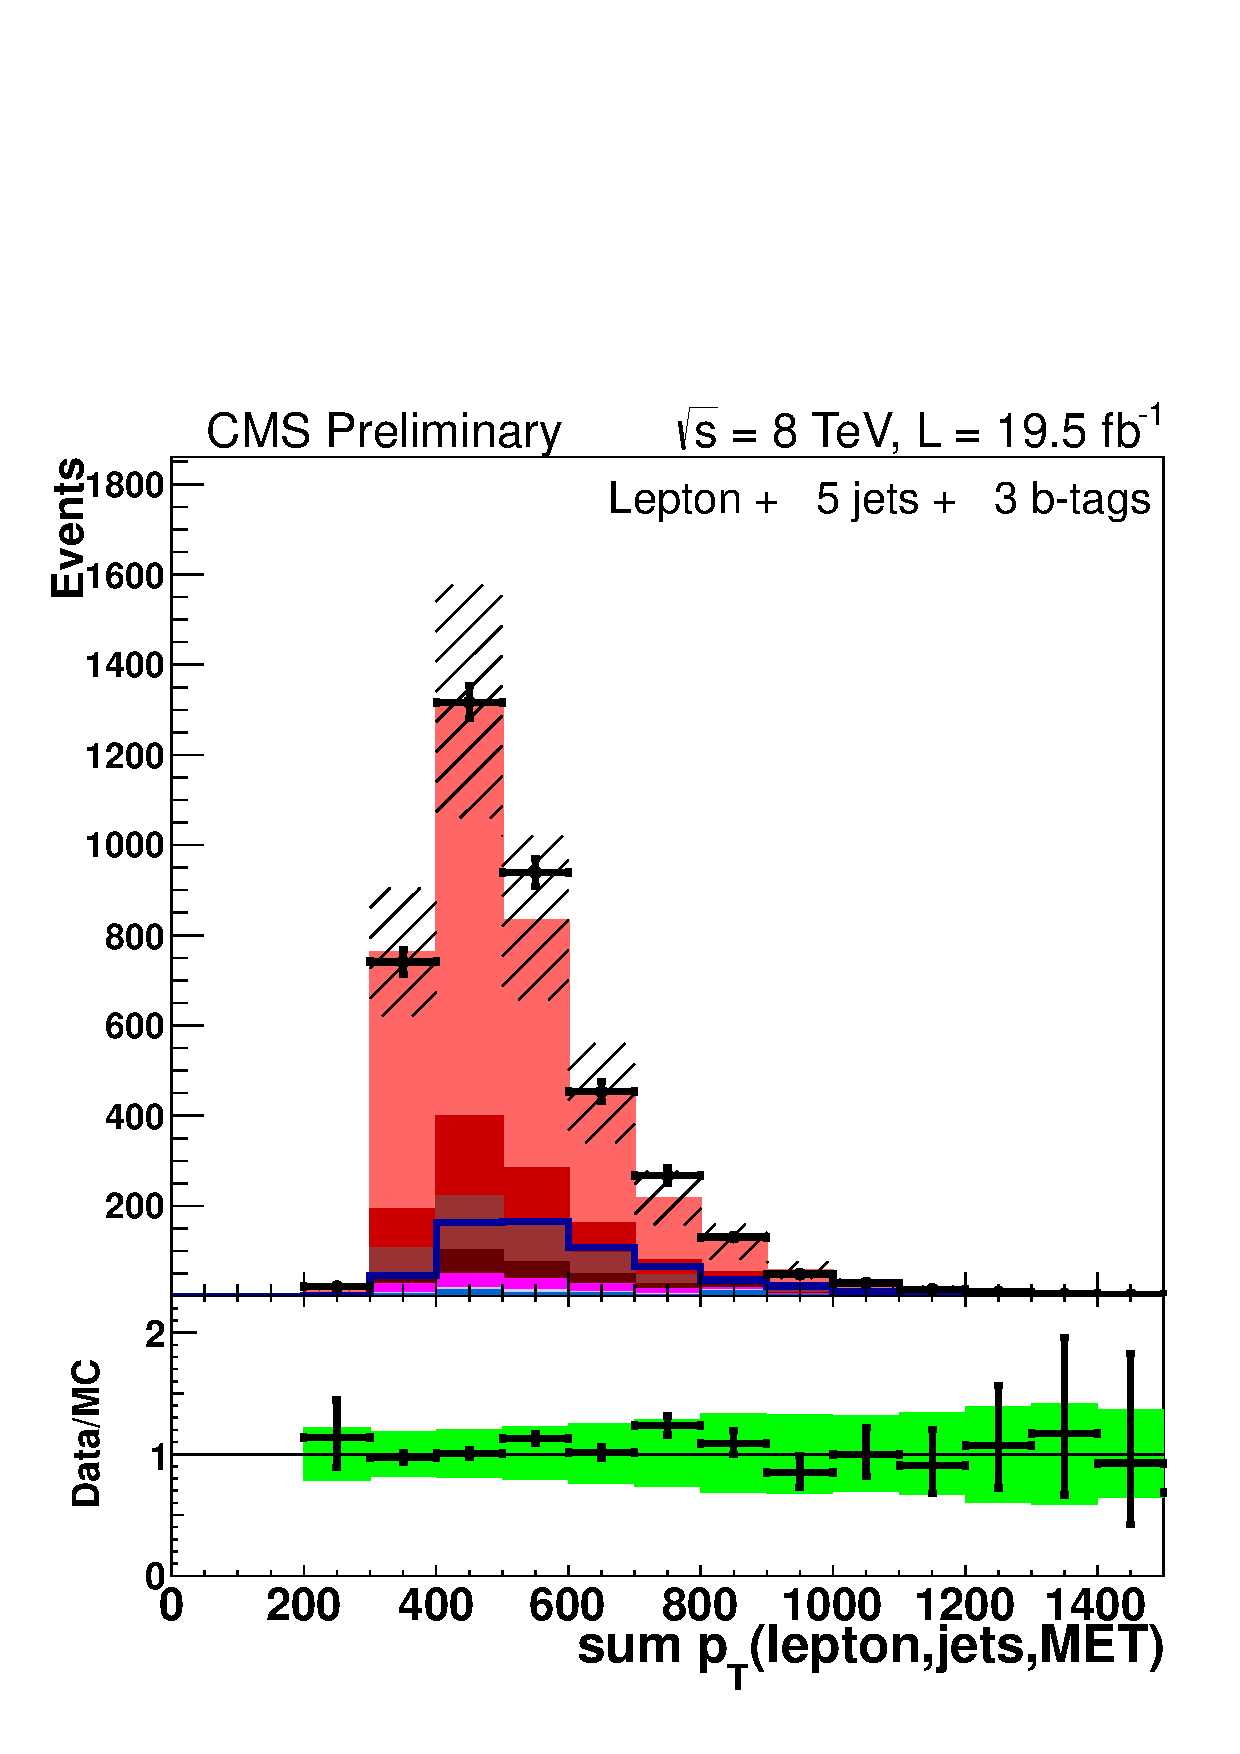
\includegraphics[width=0.31\textwidth]{Figures/Analysis_2_Diagrams/LJ_plots_lep/5j3t/lep_all_sum_pt_with_met_5j3t_cumulative_wRatio_noLegend_lin.pdf}
   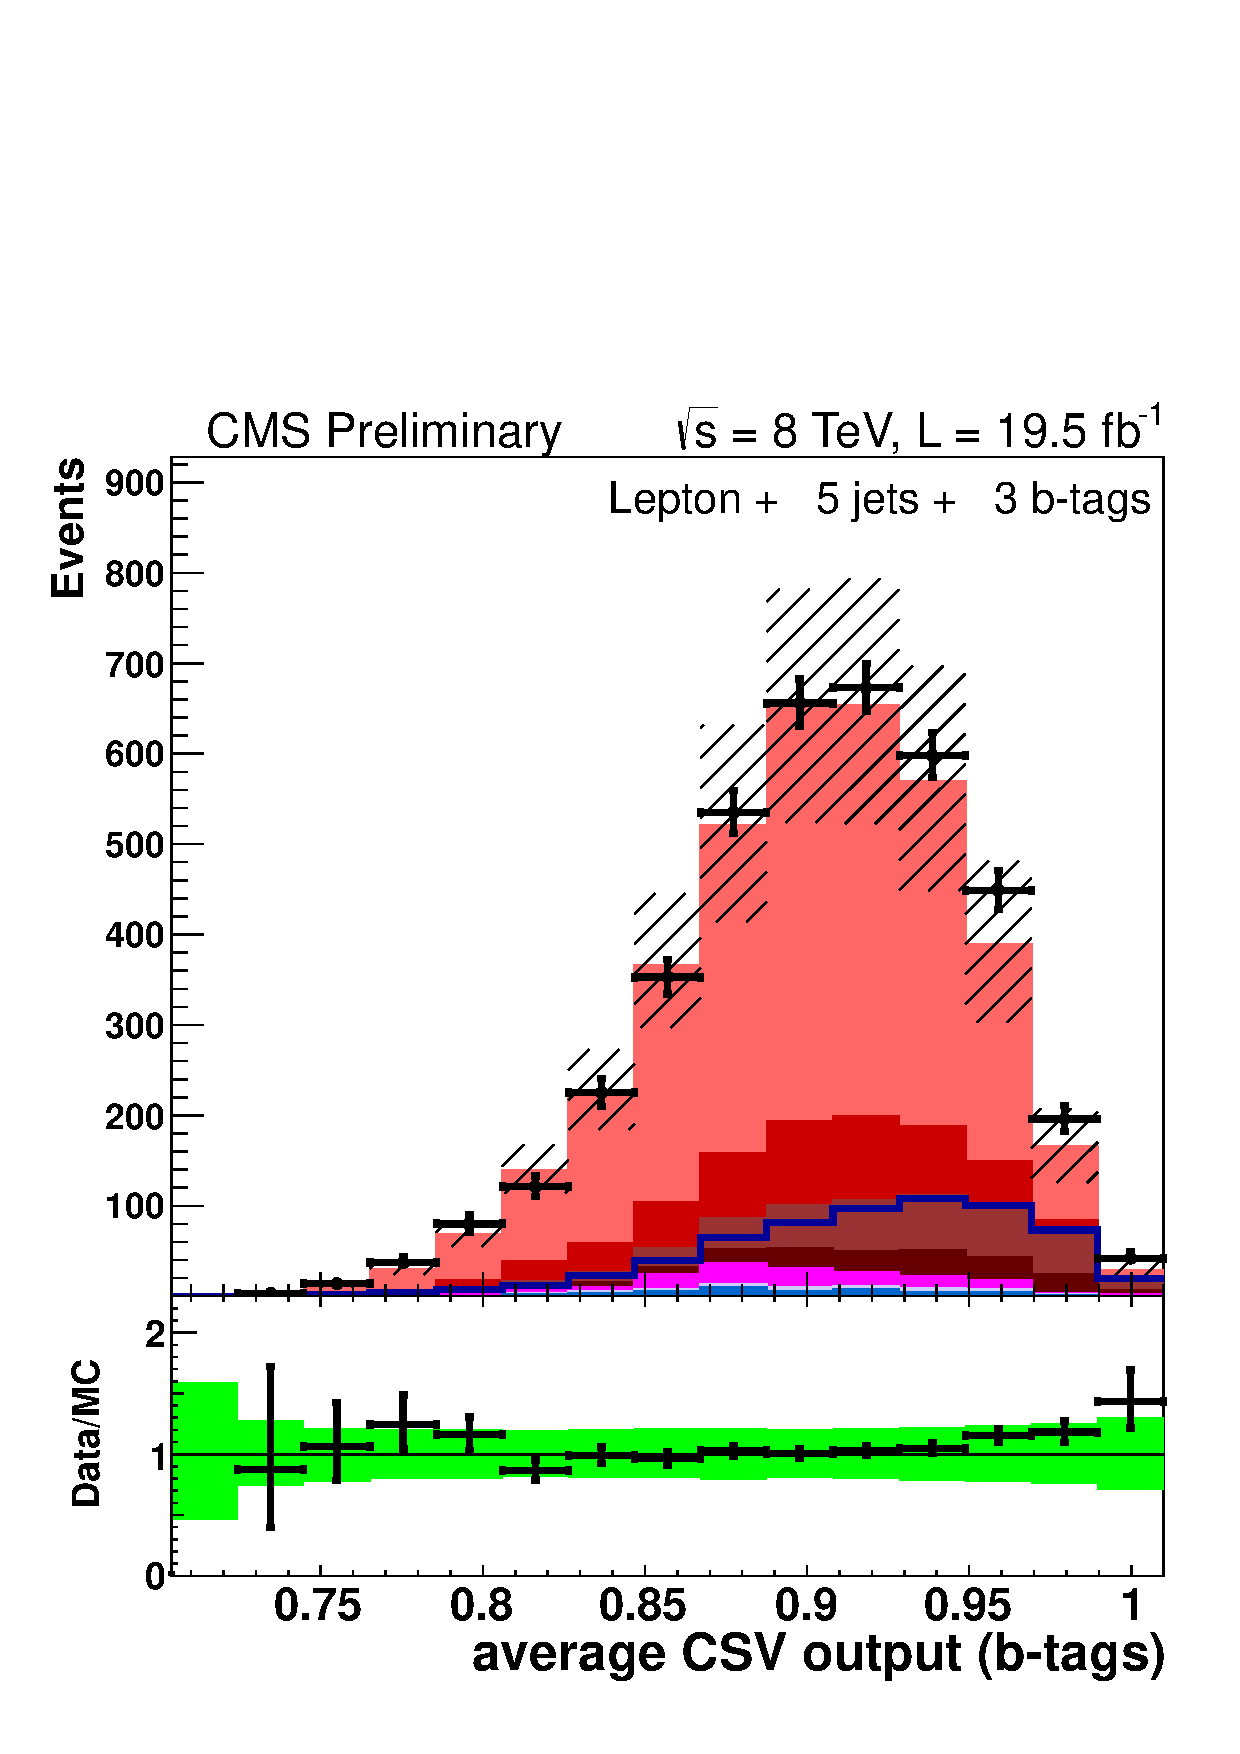
\includegraphics[width=0.31\textwidth]{Figures/Analysis_2_Diagrams/LJ_plots_lep/5j3t/lep_avg_btag_disc_btags_5j3t_cumulative_wRatio_noLegend_lin.pdf}
   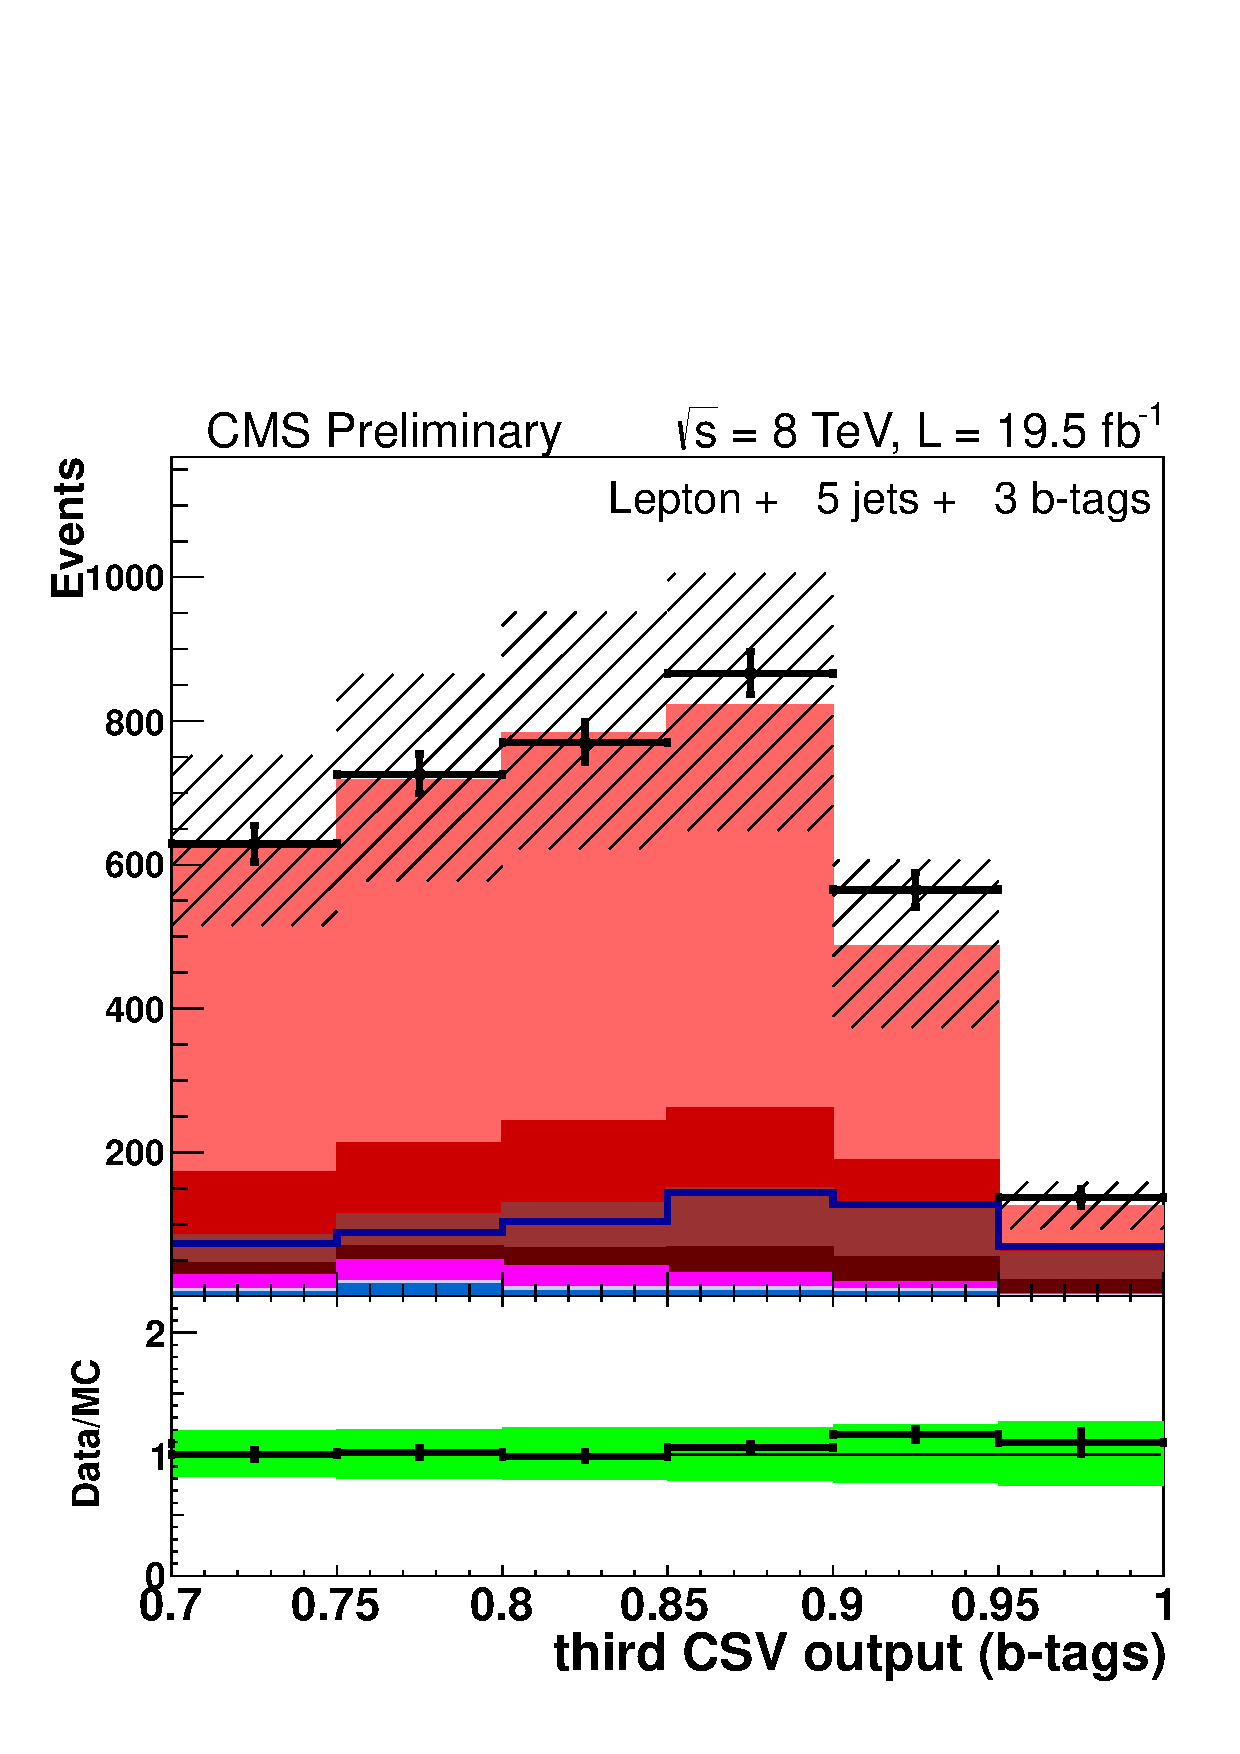
\includegraphics[width=0.31\textwidth]{Figures/Analysis_2_Diagrams/LJ_plots_lep/5j3t/lep_jet_csv_3_5j3t_cumulative_wRatio_noLegend_lin.pdf}
   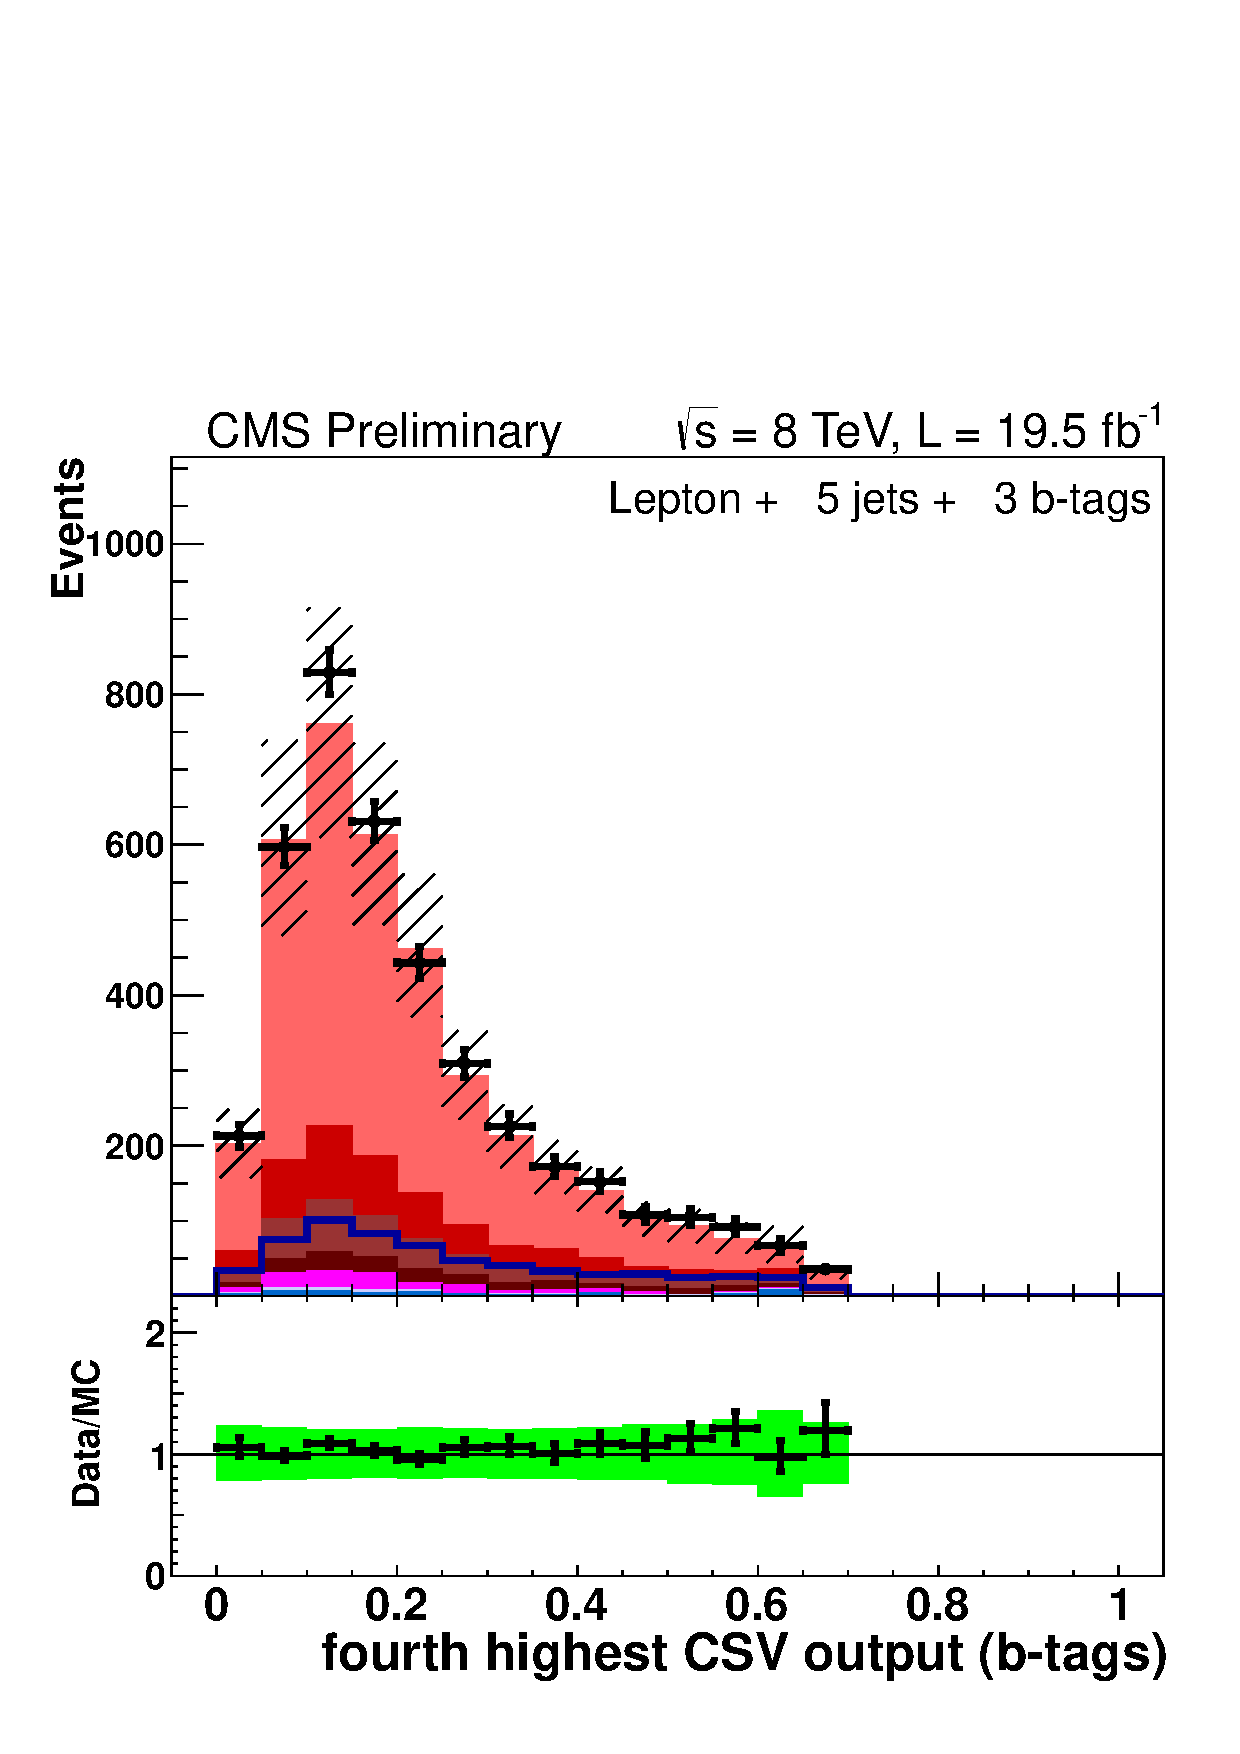
\includegraphics[width=0.31\textwidth]{Figures/Analysis_2_Diagrams/LJ_plots_lep/5j3t/lep_jet_csv_4_5j3t_cumulative_wRatio_noLegend_lin.pdf}
   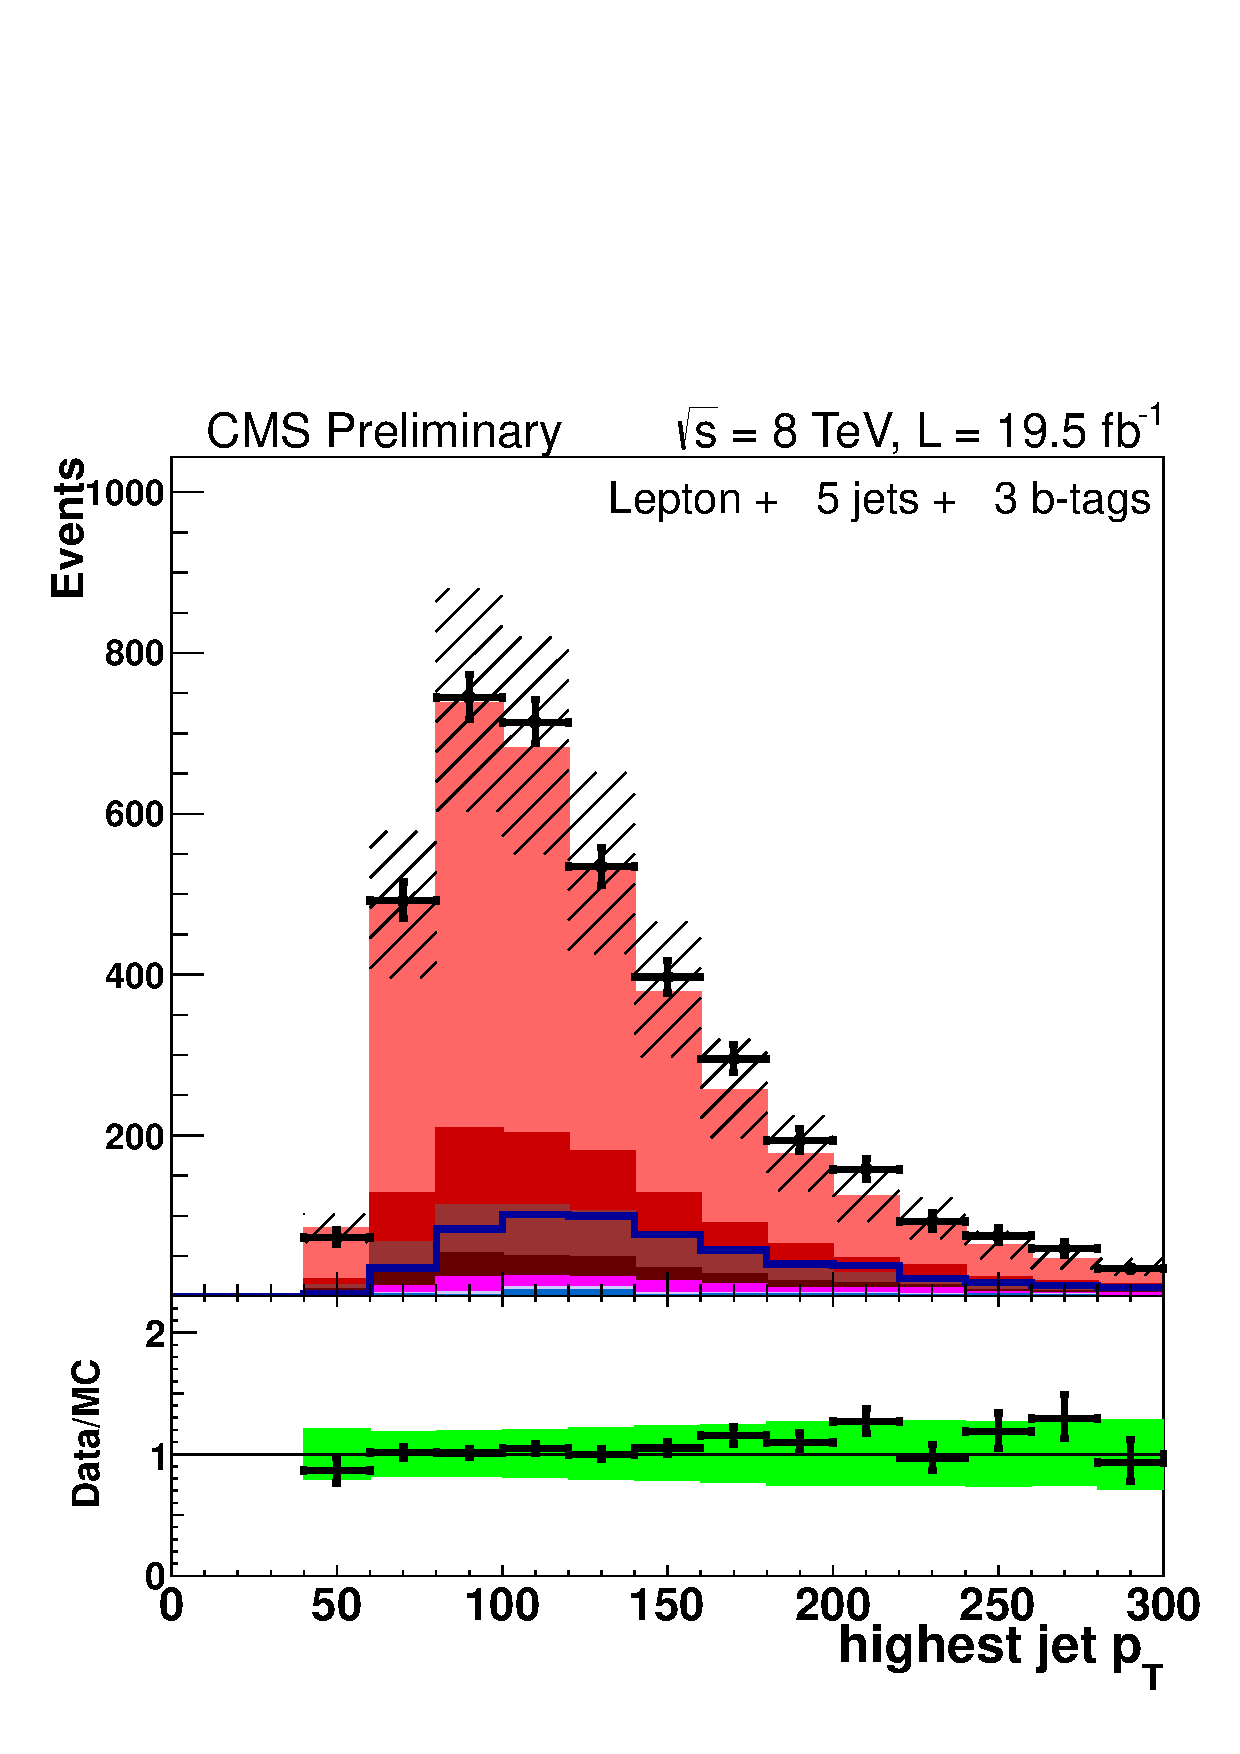
\includegraphics[width=0.31\textwidth]{Figures/Analysis_2_Diagrams/LJ_plots_lep/5j3t/lep_jet_pt_1_5j3t_cumulative_wRatio_noLegend_lin.pdf}
   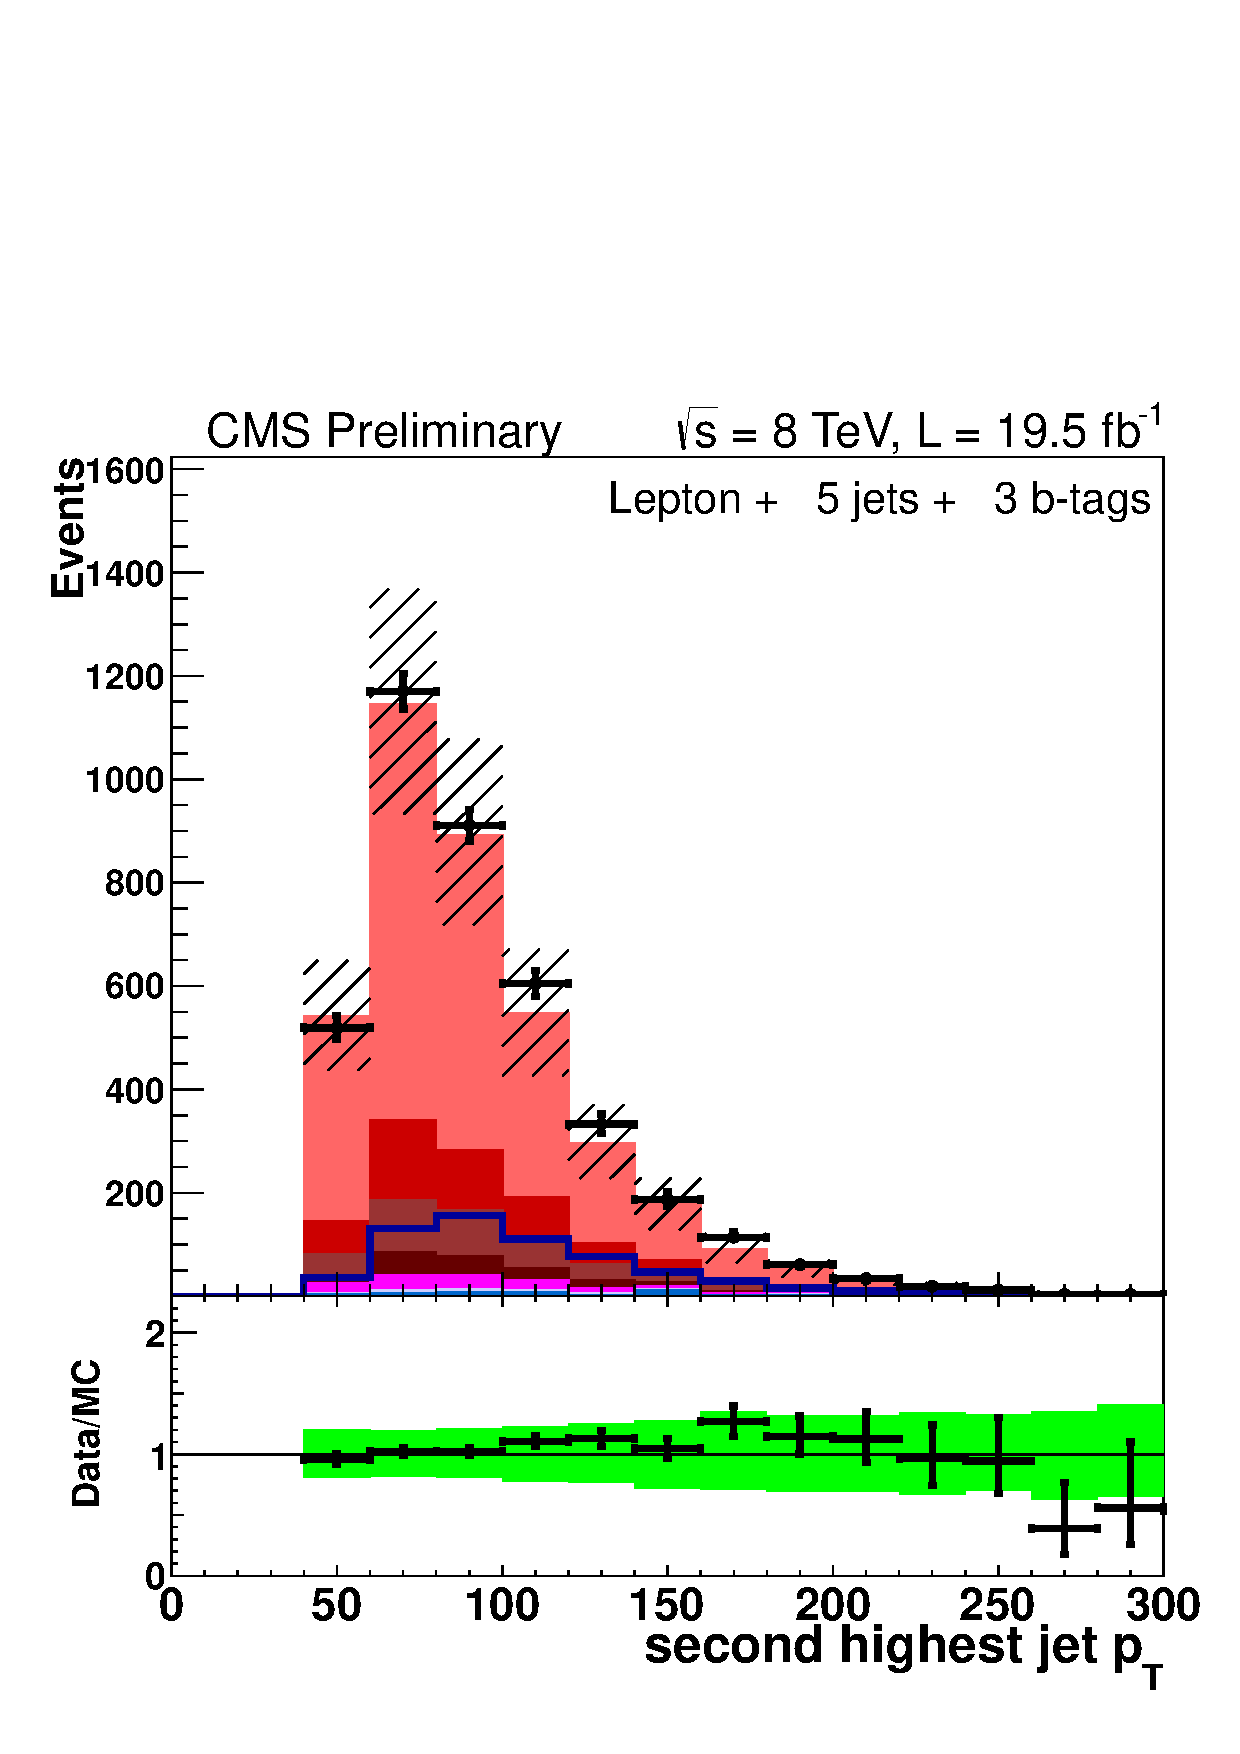
\includegraphics[width=0.31\textwidth]{Figures/Analysis_2_Diagrams/LJ_plots_lep/5j3t/lep_jet_pt_2_5j3t_cumulative_wRatio_noLegend_lin.pdf}
   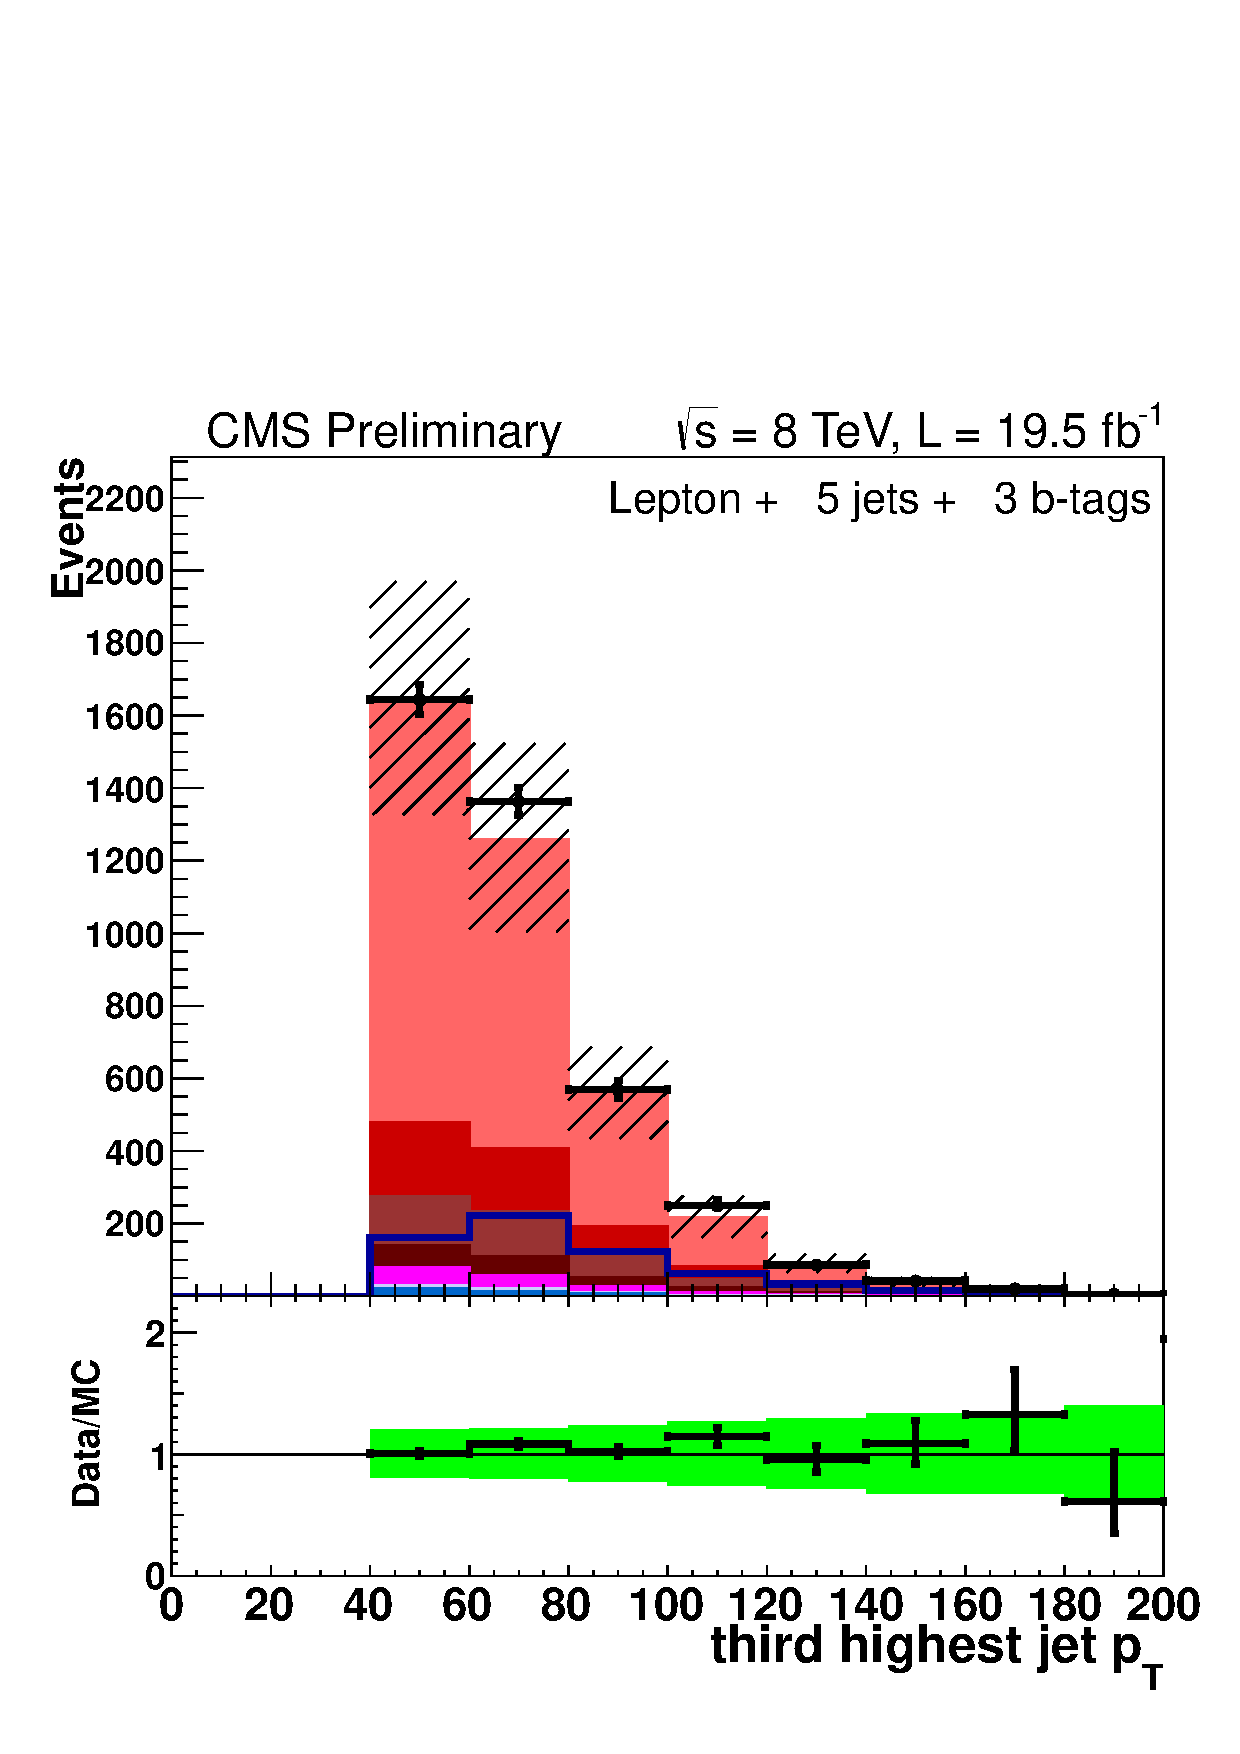
\includegraphics[width=0.31\textwidth]{Figures/Analysis_2_Diagrams/LJ_plots_lep/5j3t/lep_jet_pt_3_5j3t_cumulative_wRatio_noLegend_lin.pdf}
   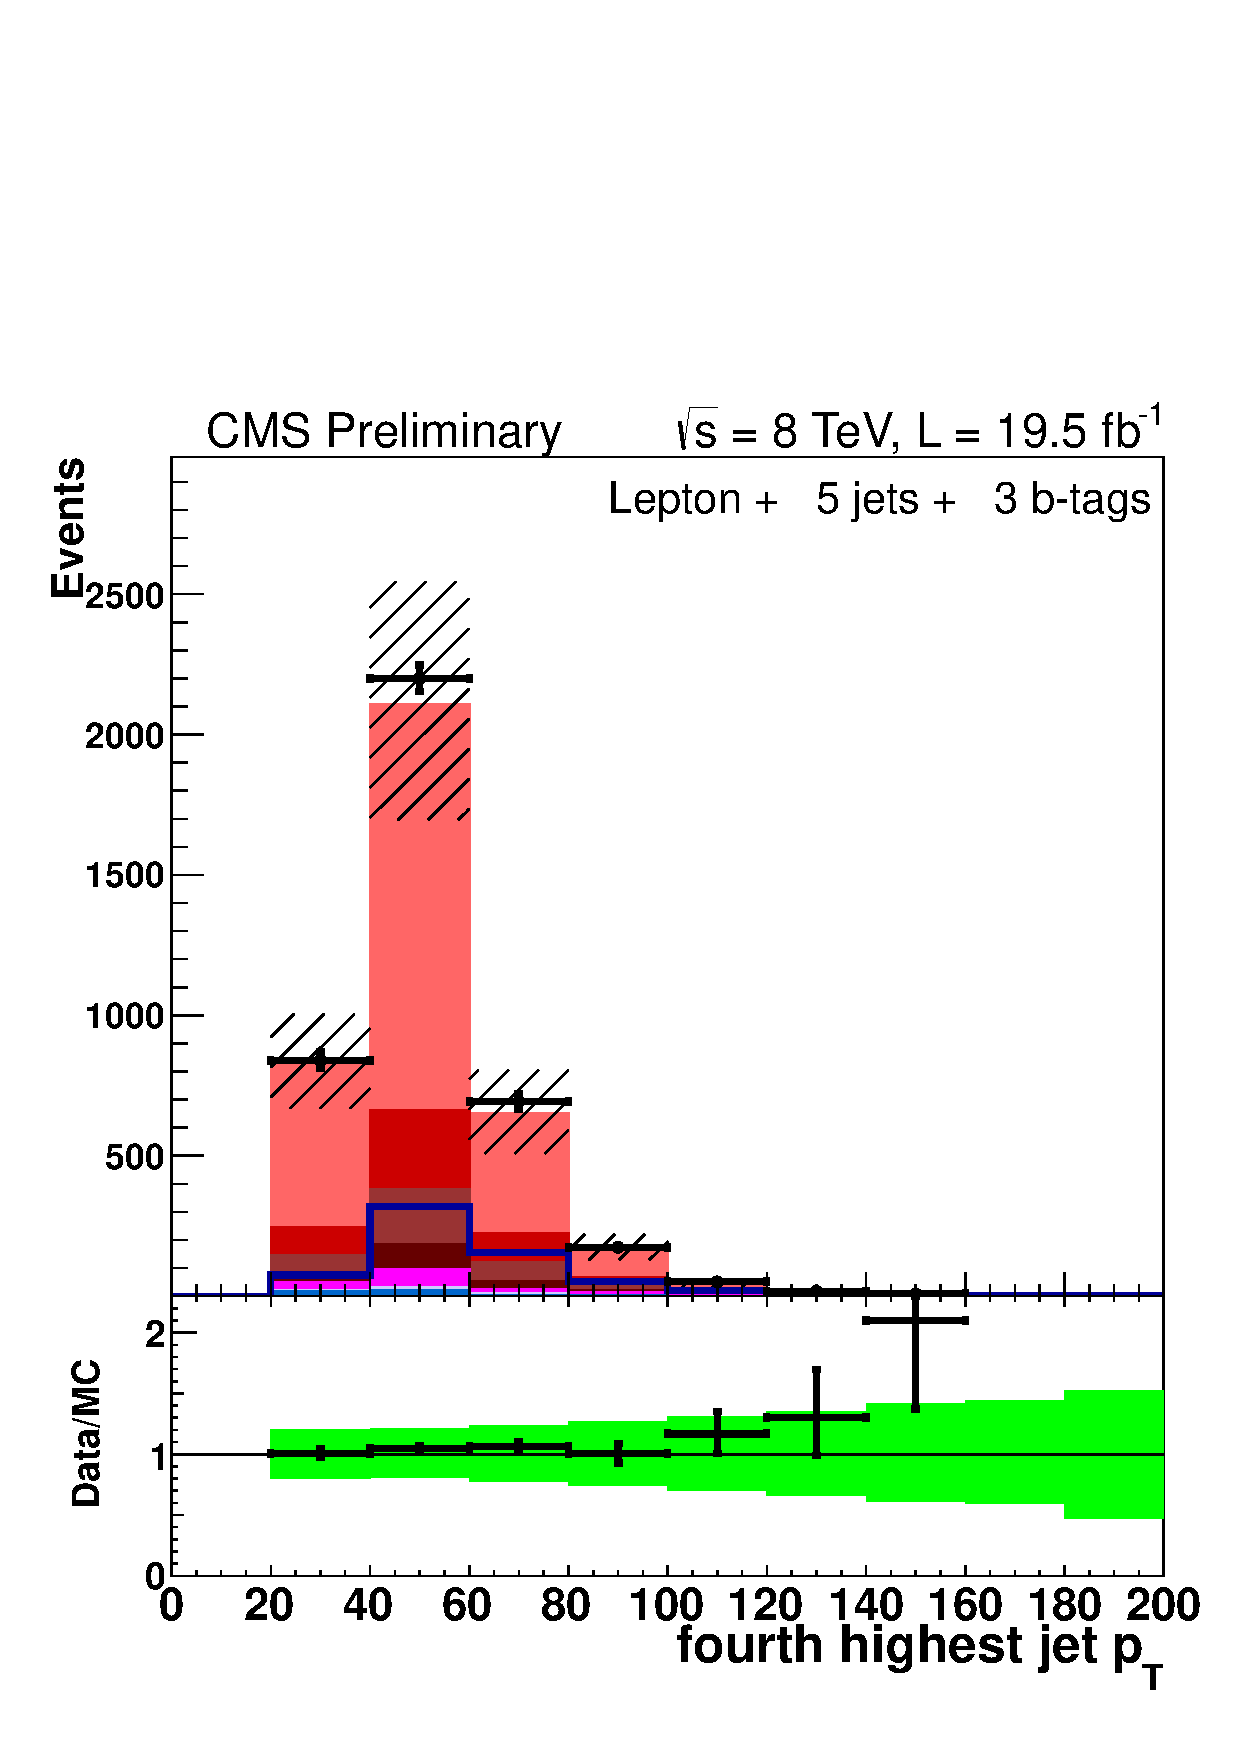
\includegraphics[width=0.31\textwidth]{Figures/Analysis_2_Diagrams/LJ_plots_lep/5j3t/lep_jet_pt_4_5j3t_cumulative_wRatio_noLegend_lin.pdf}
   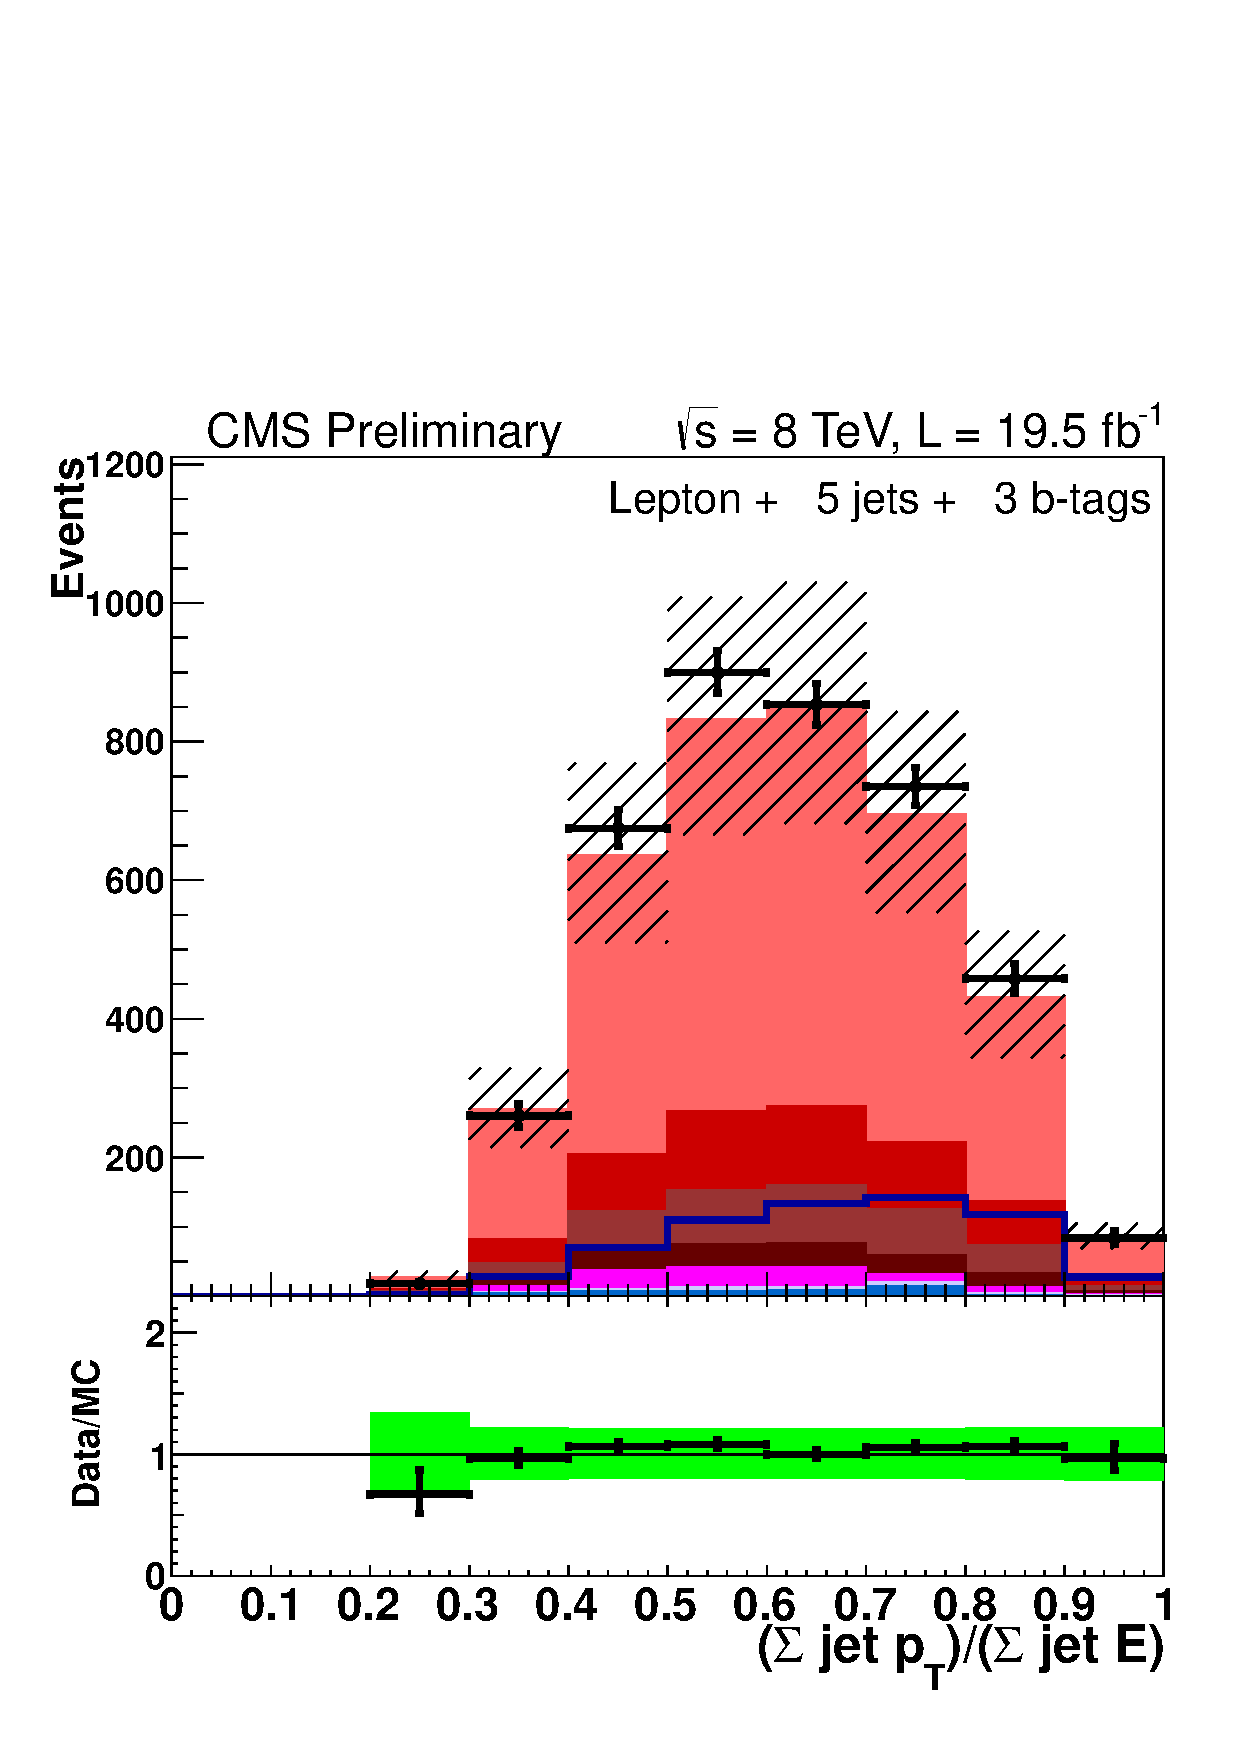
\includegraphics[width=0.31\textwidth]{Figures/Analysis_2_Diagrams/LJ_plots_lep/5j3t/lep_pt_all_jets_over_E_all_jets_5j3t_cumulative_wRatio_noLegend_lin.pdf}
   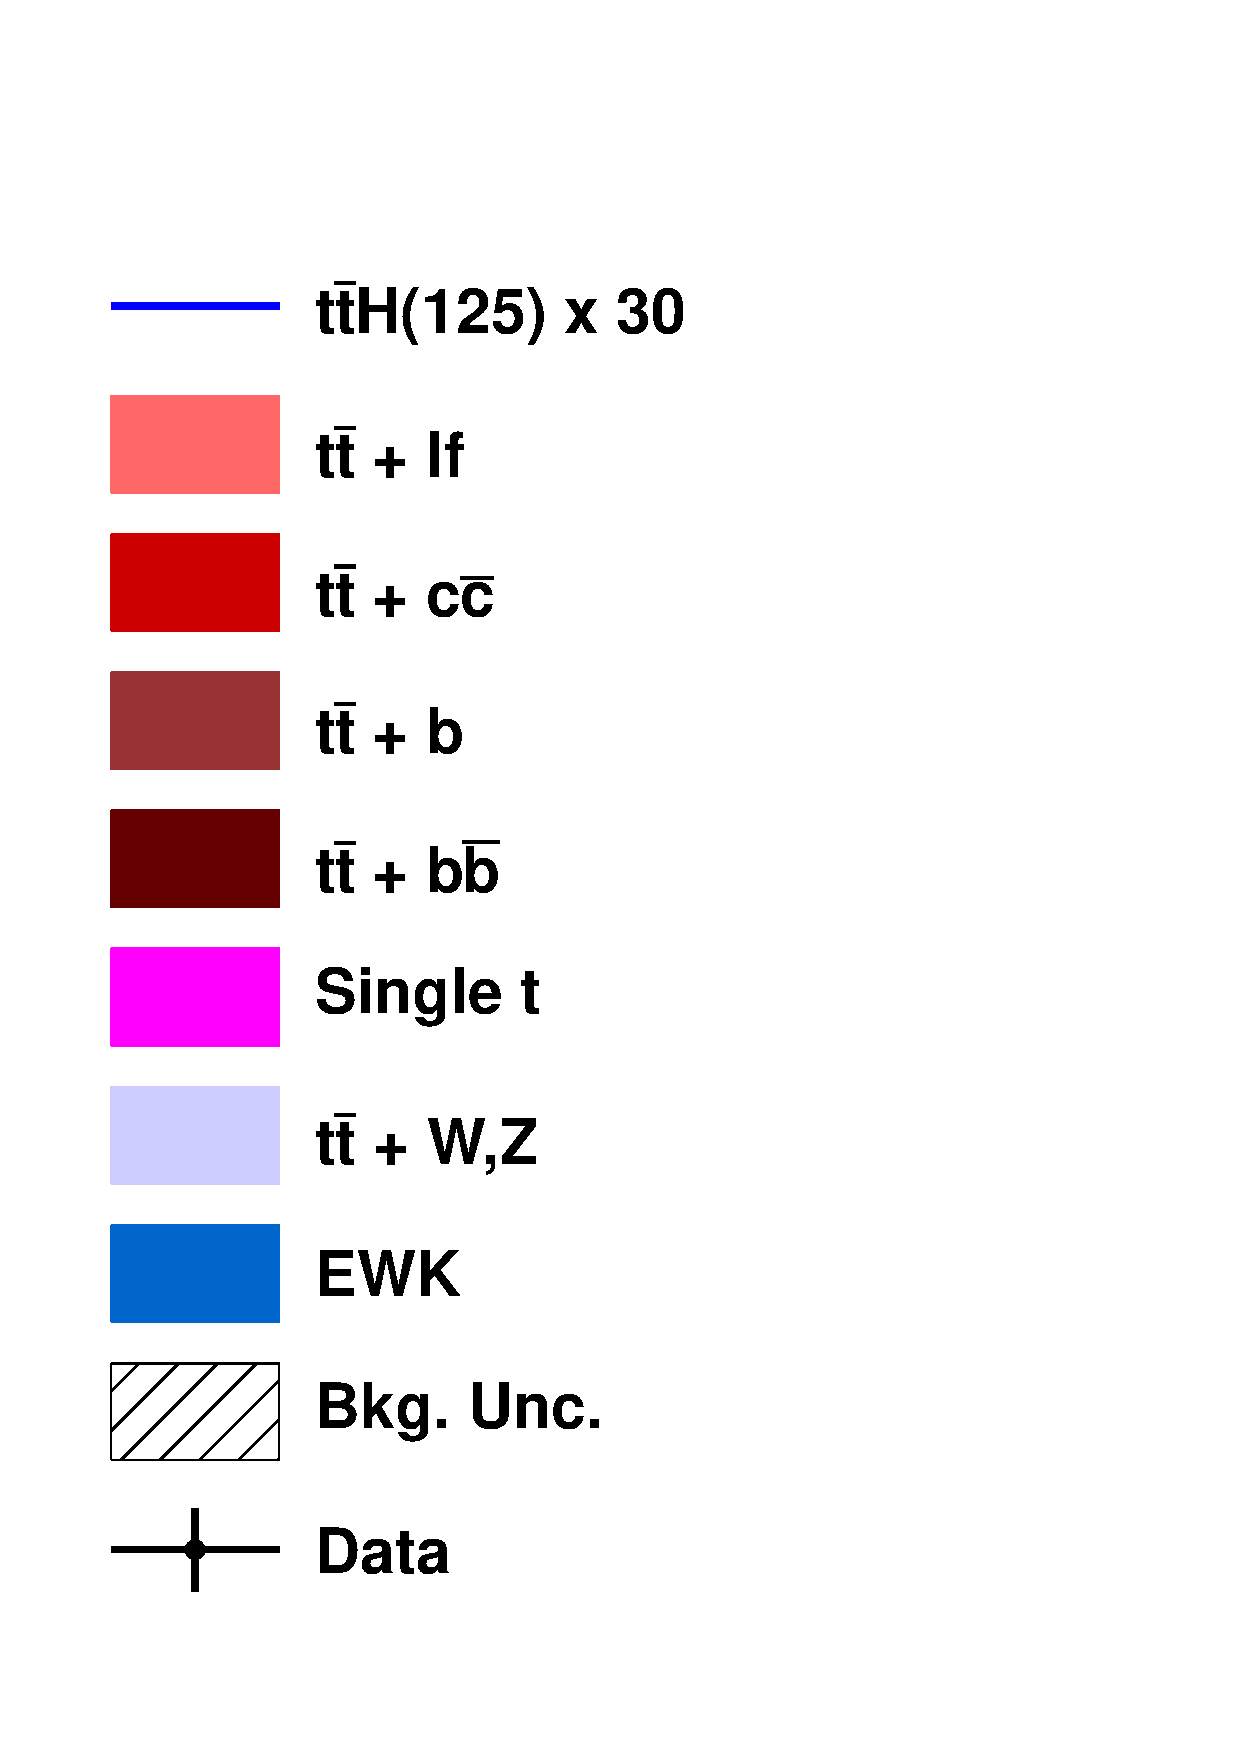
\includegraphics[width=0.15\textwidth]{Figures/Analysis_2_Diagrams/LJ_plots_lep/ttH_legend_1columns.pdf}
   \caption{Data/MC comparisons for events with one lepton and 5 jets + 3 b-tags.  The uncertainty band includes statistical and systematic uncertainties that affect both the rate and shape of the background distributions.}
   \label{fig:lj_input_II_5j3t}
 \end{center}
\end{figure}

\clearpage


\begin{figure}[hbtp]
 \begin{center}
   \includegraphics[width=0.31\textwidth]{Figures/Analysis_2_Diagrams/LJ_plots_lep/6j3t/lep_all_sum_pt_with_met_6j3t_cumulative_wRatio_noLegend_lin.pdf}
   \includegraphics[width=0.31\textwidth]{Figures/Analysis_2_Diagrams/LJ_plots_lep/6j3t/lep_avg_btag_disc_btags_6j3t_cumulative_wRatio_noLegend_lin.pdf}
   \includegraphics[width=0.31\textwidth]{Figures/Analysis_2_Diagrams/LJ_plots_lep/6j3t/lep_h0_6j3t_cumulative_wRatio_noLegend_lin.pdf}
   \includegraphics[width=0.31\textwidth]{Figures/Analysis_2_Diagrams/LJ_plots_lep/6j3t/lep_h1_6j3t_cumulative_wRatio_noLegend_lin.pdf}
   \includegraphics[width=0.31\textwidth]{Figures/Analysis_2_Diagrams/LJ_plots_lep/6j3t/lep_jet_csv_2_6j3t_cumulative_wRatio_noLegend_lin.pdf}
   \includegraphics[width=0.31\textwidth]{Figures/Analysis_2_Diagrams/LJ_plots_lep/6j3t/lep_jet_csv_3_6j3t_cumulative_wRatio_noLegend_lin.pdf}
   \includegraphics[width=0.31\textwidth]{Figures/Analysis_2_Diagrams/LJ_plots_lep/6j3t/lep_jet_csv_4_6j3t_cumulative_wRatio_noLegend_lin.pdf}
   \includegraphics[width=0.31\textwidth]{Figures/Analysis_2_Diagrams/LJ_plots_lep/6j3t/lep_maxeta_jet_jet_6j3t_cumulative_wRatio_noLegend_lin.pdf}
   \includegraphics[width=0.31\textwidth]{Figures/Analysis_2_Diagrams/LJ_plots_lep/6j3t/lep_pt_all_jets_over_E_all_jets_6j3t_cumulative_wRatio_noLegend_lin.pdf}
   \includegraphics[width=0.31\textwidth]{Figures/Analysis_2_Diagrams/LJ_plots_lep/6j3t/lep_sphericity_6j3t_cumulative_wRatio_noLegend_lin.pdf}
   \includegraphics[width=0.31\textwidth]{Figures/Analysis_2_Diagrams/LJ_plots_lep/6j3t/lep_disc_ttH_ttbb_6j3t_8TeV_CFMlpANN_BDT_6j3t_cumulative_wRatio_noLegend_lin.pdf}
   \includegraphics[width=0.15\textwidth]{Figures/Analysis_2_Diagrams/LJ_plots_lep/ttH_legend_1columns.pdf}
   \caption{Data/MC comparisons for events with one lepton and $\ge$6 jets + 3 b-tags.  The uncertainty band includes statistical and systematic uncertainties that affect both the rate and shape of the background distributions.}
   \label{fig:lj_input_II_6j3t_1}
 \end{center}
\end{figure}

\clearpage



\begin{figure}[hbtp]
 \begin{center}
   \includegraphics[width=0.31\textwidth]{Figures/Analysis_2_Diagrams/LJ_plots_lep/6j3t/lep_h3_6j3t_cumulative_wRatio_noLegend_lin.pdf}
   \includegraphics[width=0.31\textwidth]{Figures/Analysis_2_Diagrams/LJ_plots_lep/6j3t/lep_maxeta_tag_tag_6j3t_cumulative_wRatio_noLegend_lin.pdf}
   \includegraphics[width=0.31\textwidth]{Figures/Analysis_2_Diagrams/LJ_plots_lep/6j3t/lep_dEta_fn_6j3t_cumulative_wRatio_noLegend_lin.pdf}
   \includegraphics[width=0.31\textwidth]{Figures/Analysis_2_Diagrams/LJ_plots_lep/6j3t/lep_abs_dEta_hadtop_bb_6j3t_cumulative_wRatio_noLegend_lin.pdf}
   \includegraphics[width=0.31\textwidth]{Figures/Analysis_2_Diagrams/LJ_plots_lep/6j3t/lep_tagged_dijet_mass_closest_to_125_6j3t_cumulative_wRatio_noLegend_lin.pdf}
   \includegraphics[width=0.31\textwidth]{Figures/Analysis_2_Diagrams/LJ_plots_lep/6j3t/lep_M3_6j3t_cumulative_wRatio_noLegend_lin.pdf}
   \includegraphics[width=0.31\textwidth]{Figures/Analysis_2_Diagrams/LJ_plots_lep/6j3t/lep_maxeta_jet_tag_6j3t_cumulative_wRatio_noLegend_lin.pdf}
   \includegraphics[width=0.31\textwidth]{Figures/Analysis_2_Diagrams/LJ_plots_lep/6j3t/lep_abs_dEta_leptop_bb_6j3t_cumulative_wRatio_noLegend_lin.pdf}
   \includegraphics[width=0.31\textwidth]{Figures/Analysis_2_Diagrams/LJ_plots_lep/6j3t/lep_aplanarity_6j3t_cumulative_wRatio_noLegend_lin.pdf}
   \includegraphics[width=0.31\textwidth]{Figures/Analysis_2_Diagrams/LJ_plots_lep/6j3t/lep_min_dR_tag_tag_6j3t_cumulative_wRatio_noLegend_lin.pdf}
   \includegraphics[width=0.31\textwidth]{Figures/Analysis_2_Diagrams/LJ_plots_lep/6j3t/lep_jet_pt_3_6j3t_cumulative_wRatio_noLegend_lin.pdf}
   \includegraphics[width=0.15\textwidth]{Figures/Analysis_2_Diagrams/LJ_plots_lep/ttH_legend_1columns.pdf}
   \caption{Data/MC comparisons for events with one lepton and $\ge$6 jets + 3 b-tags.  The uncertainty band includes statistical and systematic uncertainties that affect both the rate and shape of the background distributions.}
   \label{fig:lj_input_II_6j3t_2}
 \end{center}
\end{figure}

\clearpage





\begin{figure}[hbtp]
 \begin{center}
   \includegraphics[width=0.31\textwidth]{Figures/Analysis_2_Diagrams/LJ_plots_lep/4j4t/lep_HT_4j4t_cumulative_wRatio_noLegend_lin.pdf}
   \includegraphics[width=0.31\textwidth]{Figures/Analysis_2_Diagrams/LJ_plots_lep/4j4t/lep_M3_4j4t_cumulative_wRatio_noLegend_lin.pdf}
   \includegraphics[width=0.31\textwidth]{Figures/Analysis_2_Diagrams/LJ_plots_lep/4j4t/lep_all_sum_pt_with_met_4j4t_cumulative_wRatio_noLegend_lin.pdf}
   \includegraphics[width=0.31\textwidth]{Figures/Analysis_2_Diagrams/LJ_plots_lep/4j4t/lep_avg_btag_disc_btags_4j4t_cumulative_wRatio_noLegend_lin.pdf}
   \includegraphics[width=0.31\textwidth]{Figures/Analysis_2_Diagrams/LJ_plots_lep/4j4t/lep_jet_csv_2_4j4t_cumulative_wRatio_noLegend_lin.pdf}
   \includegraphics[width=0.31\textwidth]{Figures/Analysis_2_Diagrams/LJ_plots_lep/4j4t/lep_jet_csv_3_4j4t_cumulative_wRatio_noLegend_lin.pdf}
   \includegraphics[width=0.31\textwidth]{Figures/Analysis_2_Diagrams/LJ_plots_lep/4j4t/lep_jet_csv_4_4j4t_cumulative_wRatio_noLegend_lin.pdf}
   \includegraphics[width=0.31\textwidth]{Figures/Analysis_2_Diagrams/LJ_plots_lep/4j4t/lep_jet_pt_1_4j4t_cumulative_wRatio_noLegend_lin.pdf}
   \includegraphics[width=0.31\textwidth]{Figures/Analysis_2_Diagrams/LJ_plots_lep/4j4t/lep_jet_pt_2_4j4t_cumulative_wRatio_noLegend_lin.pdf}
   \includegraphics[width=0.31\textwidth]{Figures/Analysis_2_Diagrams/LJ_plots_lep/4j4t/lep_jet_pt_4_4j4t_cumulative_wRatio_noLegend_lin.pdf}
   \includegraphics[width=0.15\textwidth]{Figures/Analysis_2_Diagrams/LJ_plots_lep/ttH_legend_1columns.pdf}
   \caption{Data/MC comparisons for events with one lepton and 4 jets + 4 b-tags.  The uncertainty band includes statistical and systematic uncertainties that affect both the rate and shape of the background distributions.}
   \label{fig:lj_input_II_4j4t}
 \end{center}
\end{figure}

\clearpage


\begin{figure}[hbtp]
 \begin{center}
   \includegraphics[width=0.31\textwidth]{Figures/Analysis_2_Diagrams/LJ_plots_lep/5j4t/lep_all_sum_pt_with_met_5j4t_cumulative_wRatio_noLegend_lin.pdf}
   \includegraphics[width=0.31\textwidth]{Figures/Analysis_2_Diagrams/LJ_plots_lep/5j4t/lep_ave_dR_tag_tag_5j4t_cumulative_wRatio_noLegend_lin.pdf}
   \includegraphics[width=0.31\textwidth]{Figures/Analysis_2_Diagrams/LJ_plots_lep/5j4t/lep_avg_btag_disc_btags_5j4t_cumulative_wRatio_noLegend_lin.pdf}
   \includegraphics[width=0.31\textwidth]{Figures/Analysis_2_Diagrams/LJ_plots_lep/5j4t/lep_dev_from_avg_disc_btags_5j4t_cumulative_wRatio_noLegend_lin.pdf}
   \includegraphics[width=0.31\textwidth]{Figures/Analysis_2_Diagrams/LJ_plots_lep/5j4t/lep_jet_csv_2_5j4t_cumulative_wRatio_noLegend_lin.pdf}
   \includegraphics[width=0.31\textwidth]{Figures/Analysis_2_Diagrams/LJ_plots_lep/5j4t/lep_jet_csv_3_5j4t_cumulative_wRatio_noLegend_lin.pdf}
   \includegraphics[width=0.31\textwidth]{Figures/Analysis_2_Diagrams/LJ_plots_lep/5j4t/lep_lowest_btag_5j4t_cumulative_wRatio_noLegend_lin.pdf}
   %\includegraphics[width=0.31\textwidth]{Figures/Analysis_2_Diagrams/LJ_plots_lep/5j4t/lep_maxeta_jet_tag_5j4t_cumulative_wRatio_noLegend_lin.pdf}
   %\includegraphics[width=0.31\textwidth]{Figures/Analysis_2_Diagrams/LJ_plots_lep/5j4t/lep_maxeta_tag_tag_5j4t_cumulative_wRatio_noLegend_lin.pdf}
   \includegraphics[width=0.31\textwidth]{Figures/Analysis_2_Diagrams/LJ_plots_lep/5j4t/lep_pt_all_jets_over_E_all_jets_5j4t_cumulative_wRatio_noLegend_lin.pdf}
   \includegraphics[width=0.31\textwidth]{Figures/Analysis_2_Diagrams/LJ_plots_lep/5j4t/lep_disc_ttH_ttbb_5j4t_8TeV_CFMlpANN_BDT_5j4t_cumulative_wRatio_noLegend_lin.pdf}
   \includegraphics[width=0.15\textwidth]{Figures/Analysis_2_Diagrams/LJ_plots_lep/ttH_legend_1columns.pdf}
   \caption{Data/MC comparisons for events with one lepton and 5 jets +$\ge$4 b-tags.  The uncertainty band includes statistical and systematic uncertainties that affect both the rate and shape of the background distributions.}
   \label{fig:lj_input_II_5j4t_1}
 \end{center}
\end{figure}

\clearpage


\begin{figure}[hbtp]
 \begin{center}
   \includegraphics[width=0.31\textwidth]{Figures/Analysis_2_Diagrams/LJ_plots_lep/5j4t/lep_maxeta_jet_tag_5j4t_cumulative_wRatio_noLegend_lin.pdf}
   \includegraphics[width=0.31\textwidth]{Figures/Analysis_2_Diagrams/LJ_plots_lep/5j4t/lep_maxeta_tag_tag_5j4t_cumulative_wRatio_noLegend_lin.pdf}
   \includegraphics[width=0.31\textwidth]{Figures/Analysis_2_Diagrams/LJ_plots_lep/5j4t/lep_h1_5j4t_cumulative_wRatio_noLegend_lin.pdf}
   \includegraphics[width=0.31\textwidth]{Figures/Analysis_2_Diagrams/LJ_plots_lep/5j4t/lep_tagged_dijet_mass_closest_to_125_5j4t_cumulative_wRatio_noLegend_lin.pdf}  
   \includegraphics[width=0.31\textwidth]{Figures/Analysis_2_Diagrams/LJ_plots_lep/5j4t/lep_jet_csv_4_5j4t_cumulative_wRatio_noLegend_lin.pdf}
   \includegraphics[width=0.31\textwidth]{Figures/Analysis_2_Diagrams/LJ_plots_lep/5j4t/lep_aplanarity_5j4t_cumulative_wRatio_noLegend_lin.pdf}
   \includegraphics[width=0.31\textwidth]{Figures/Analysis_2_Diagrams/LJ_plots_lep/5j4t/lep_h3_5j4t_cumulative_wRatio_noLegend_lin.pdf}
   \includegraphics[width=0.31\textwidth]{Figures/Analysis_2_Diagrams/LJ_plots_lep/5j4t/lep_met_pt_5j4t_cumulative_wRatio_noLegend_lin.pdf}
   \includegraphics[width=0.15\textwidth]{Figures/Analysis_2_Diagrams/LJ_plots_lep/ttH_legend_1columns.pdf}
   \caption{Data/MC comparisons for events with one lepton and 5 jets +$\ge$4 b-tags.  The uncertainty band includes statistical and systematic uncertainties that affect both the rate and shape of the background distributions.}
   \label{fig:lj_input_II_5j4t_2}
 \end{center}
\end{figure}

\clearpage





\begin{figure}[hbtp]
 \begin{center}
   \includegraphics[width=0.31\textwidth]{Figures/Analysis_2_Diagrams/LJ_plots_lep/6j4t/lep_abs_dEta_hadtop_bb_6j4t_cumulative_wRatio_noLegend_lin.pdf}
   \includegraphics[width=0.31\textwidth]{Figures/Analysis_2_Diagrams/LJ_plots_lep/6j4t/lep_abs_dEta_leptop_bb_6j4t_cumulative_wRatio_noLegend_lin.pdf}
   \includegraphics[width=0.31\textwidth]{Figures/Analysis_2_Diagrams/LJ_plots_lep/6j4t/lep_ave_dR_tag_tag_6j4t_cumulative_wRatio_noLegend_lin.pdf}
   \includegraphics[width=0.31\textwidth]{Figures/Analysis_2_Diagrams/LJ_plots_lep/6j4t/lep_avg_btag_disc_btags_6j4t_cumulative_wRatio_noLegend_lin.pdf}
   \includegraphics[width=0.31\textwidth]{Figures/Analysis_2_Diagrams/LJ_plots_lep/6j4t/lep_best_higgs_mass_6j4t_cumulative_wRatio_noLegend_lin.pdf}
   \includegraphics[width=0.31\textwidth]{Figures/Analysis_2_Diagrams/LJ_plots_lep/6j4t/lep_closest_tagged_dijet_mass_6j4t_cumulative_wRatio_noLegend_lin.pdf}
   \includegraphics[width=0.31\textwidth]{Figures/Analysis_2_Diagrams/LJ_plots_lep/6j4t/lep_dEta_fn_6j4t_cumulative_wRatio_noLegend_lin.pdf}
   \includegraphics[width=0.31\textwidth]{Figures/Analysis_2_Diagrams/LJ_plots_lep/6j4t/lep_dRbb_6j4t_cumulative_wRatio_noLegend_lin.pdf}
   \includegraphics[width=0.31\textwidth]{Figures/Analysis_2_Diagrams/LJ_plots_lep/6j4t/lep_disc_ttH_ttbb_best15_8TeV_CFMlpANN_BDT_6j4t_cumulative_wRatio_noLegend_lin.pdf}
   \includegraphics[width=0.15\textwidth]{Figures/Analysis_2_Diagrams/LJ_plots_lep/ttH_legend_1columns.pdf}
   \caption{Data/MC comparisons for events with one lepton and $\ge$6 jets + $\ge$4 b-tags.  The uncertainty band includes statistical and systematic uncertainties that affect both the rate and shape of the background distributions.}
   \label{fig:lj_input_II_6j4t_1}
 \end{center}
\end{figure}			

\clearpage


\begin{figure}[hbtp]
 \begin{center}
   \includegraphics[width=0.31\textwidth]{Figures/Analysis_2_Diagrams/LJ_plots_lep/6j4t/lep_h3_6j4t_cumulative_wRatio_noLegend_lin.pdf}
   \includegraphics[width=0.31\textwidth]{Figures/Analysis_2_Diagrams/LJ_plots_lep/6j4t/lep_invariant_mass_of_everything_6j4t_cumulative_wRatio_noLegend_lin.pdf}
   \includegraphics[width=0.31\textwidth]{Figures/Analysis_2_Diagrams/LJ_plots_lep/6j4t/lep_jet_csv_3_6j4t_cumulative_wRatio_noLegend_lin.pdf}
   \includegraphics[width=0.31\textwidth]{Figures/Analysis_2_Diagrams/LJ_plots_lep/6j4t/lep_jet_csv_4_6j4t_cumulative_wRatio_noLegend_lin.pdf}
   \includegraphics[width=0.31\textwidth]{Figures/Analysis_2_Diagrams/LJ_plots_lep/6j4t/lep_maxeta_jet_tag_6j4t_cumulative_wRatio_noLegend_lin.pdf}
   \includegraphics[width=0.31\textwidth]{Figures/Analysis_2_Diagrams/LJ_plots_lep/6j4t/lep_maxeta_tag_tag_6j4t_cumulative_wRatio_noLegend_lin.pdf}
   \includegraphics[width=0.31\textwidth]{Figures/Analysis_2_Diagrams/LJ_plots_lep/6j4t/lep_median_bb_mass_6j4t_cumulative_wRatio_noLegend_lin.pdf}
   \includegraphics[width=0.31\textwidth]{Figures/Analysis_2_Diagrams/LJ_plots_lep/6j4t/lep_pt_all_jets_over_E_all_jets_6j4t_cumulative_wRatio_noLegend_lin.pdf}
   \includegraphics[width=0.31\textwidth]{Figures/Analysis_2_Diagrams/LJ_plots_lep/6j4t/lep_sphericity_6j4t_cumulative_wRatio_noLegend_lin.pdf}
   \includegraphics[width=0.15\textwidth]{Figures/Analysis_2_Diagrams/LJ_plots_lep/ttH_legend_1columns.pdf}
   \caption{Data/MC comparisons for events with one lepton and $\ge$6 jets + $\ge$4 b-tags.  The uncertainty band includes statistical and systematic uncertainties that affect both the rate and shape of the background distributions.}
   \label{fig:lj_input_II_6j4t_2}
 \end{center}
\end{figure}

\clearpage




\subsection{MVA Output, Data to Monte Carlo Comparisons}
\label{mva_input_vars_data_to_mc_II_overview}

\par The distributions of the BDT output discriminators in each category are shown in
Fig.~\ref{fig:lj_BDToutput_comb}.  For these figures, the uncertainty band includes
statistical and systematic uncertainties, e.g. JES and $b$-tag SF
uncertainties, that are described in section \ref{systematics_II_overview}.

\begin{figure}[hbtp]
  \centering
  
  \begin{subfigure}[hbtp]{0.31\textwidth}
     \includegraphics[width=\textwidth]{Figures/Analysis_2_Diagrams/LJ_plots_lep/4j3t/lep_disc_final10v16_8TeV_CFMlpANN_BDT_4j3t_cumulative_wRatio_noLegend_lin.pdf}
     \caption{4 jets, 3 $b$-tags}\label{lj_BDToutput_8TeV_1}
   \end{subfigure}
   ~ %add desired spacing between images, e. g. ~, \quad, \qquad, \hfill etc.
      % (or a blank line to force the subfigure onto a new line)
   \begin{subfigure}[hbtp]{0.31\textwidth}
     \includegraphics[width=\textwidth]{Figures/Analysis_2_Diagrams/LJ_plots_lep/4j4t/lep_disc_final10v16_8TeV_CFMlpANN_BDT_4j4t_cumulative_wRatio_noLegend_lin.pdf}
     \caption{4 jets, 4 $b$-tags}\label{lj_BDToutput_8TeV_2}
   \end{subfigure}
   ~ %add desired spacing between images, e. g. ~, \quad, \qquad, \hfill etc.
      % (or a blank line to force the subfigure onto a new line)
   \begin{subfigure}[hbtp]{0.31\textwidth}
     \includegraphics[width=\textwidth]{Figures/Analysis_2_Diagrams/LJ_plots_lep/5j3t/lep_disc_final10v16_8TeV_CFMlpANN_BDT_5j3t_cumulative_wRatio_noLegend_lin.pdf}
     \caption{5 jets, 3 $b$-tags}\label{lj_BDToutput_8TeV_3}
   \end{subfigure}
   ~ %add desired spacing between images, e. g. ~, \quad, \qquad, \hfill etc.
      % (or a blank line to force the subfigure onto a new line)
   \begin{subfigure}[hbtp]{0.31\textwidth}
     \includegraphics[width=\textwidth]{Figures/Analysis_2_Diagrams/LJ_plots_lep/5j4t/lep_disc_final10v16_8TeV_CFMlpANN_BDT_5j4t_cumulative_wRatio_noLegend_lin.pdf}
     \caption{5 jets, $\ge$4 $b$-tags}\label{lj_BDToutput_8TeV_4}
   \end{subfigure}
   ~ %add desired spacing between images, e. g. ~, \quad, \qquad, \hfill etc.
      % (or a blank line to force the subfigure onto a new line)
   \begin{subfigure}[hbtp]{0.31\textwidth}
     \includegraphics[width=\textwidth]{Figures/Analysis_2_Diagrams/LJ_plots_lep/6j2t/lep_disc_final10v16_8TeV_CFMlpANN_BDT_6j2t_cumulative_wRatio_noLegend_lin.pdf}
     \caption{$\ge$6 jets, 3 $b$-tags}\label{lj_BDToutput_8TeV_5}
   \end{subfigure}
   ~ %add desired spacing between images, e. g. ~, \quad, \qquad, \hfill etc.
   % (or a blank line to force the subfigure onto a new line)
   \begin{subfigure}[hbtp]{0.31\textwidth} 
     \includegraphics[width=\textwidth]{Figures/Analysis_2_Diagrams/LJ_plots_lep/6j3t/lep_disc_final10v16_8TeV_CFMlpANN_BDT_6j3t_cumulative_wRatio_noLegend_lin.pdf}
     \caption{$\ge$6 jets, 3 $b$-tags}\label{lj_BDToutput_8TeV_6}
   \end{subfigure}
   ~ %add desired spacing between images, e. g. ~, \quad, \qquad, \hfill etc.
      % (or a blank line to force the subfigure onto a new line)
   \begin{subfigure}[hbtp]{0.31\textwidth} 
     \includegraphics[width=\textwidth]{Figures/Analysis_2_Diagrams/LJ_plots_lep/6j4t/lep_disc_final10v16_8TeV_CFMlpANN_BDT_6j4t_cumulative_wRatio_noLegend_lin.pdf}
     \caption{$\ge$6 jets, $\ge$4 $b$-tags}\label{lj_BDToutput_8TeV_7}
   \end{subfigure}
   ~ %add desired spacing between images, e. g. ~, \quad, \qquad, \hfill etc.
      % (or a blank line to force the subfigure onto a new line)
   \begin{subfigure}[hbtp]{0.15\textwidth}
     \raisebox{0.1\height}{\includegraphics[width=\textwidth]{Figures/Analysis_2_Diagrams/LJ_plots_lep/ttH_legend_1columns.pdf}}
     \caption{Legend}\label{lj_ANNinput_8TeV_leg5}
   \end{subfigure}
   %\hspace{0.1\textwidth}
   

   \caption{Final BDT output for lepton + jet events. Background-like
   events have a low BDT output value. Signal-like events
   have a high BDT output value.  The uncertainty band
   includes statistical and systematic uncertainties that affect both
   the rate and shape of the background distributions. The top, middle
   and, bottom rows are events with 4, 5, and $\ge$6 jets,
   respectively, while the left, middle, and right-hand columns are
   events with 2, 3, and $\ge$4 b-tags, respectively. The
   $t\bar{t}H$ signal $(m_{H} = 125 \GeV)$ is
   normalized to 30 $\times$ SM expectation.}
   \label{fig:lj_BDToutput_comb} 
\end{figure}





\section{Systematic Uncertainties}
\label{systematics_II_overview}

\par The evaluation of several of the systematic uncertainties follows
the same procedure as described in the previous chapter.  For these
cases, the reader is directed to previous description of the
uncertainty.  Systematic uncertainties that are new to this analysis
include those associated with the new $b$-tag calibration method and the
top-$p_{T}$ reweighting.  Where appropriate, comparisons between the
shapes of the nominal and $\pm1\sigma$ variations are made.  


\begin{description}

\item[Jet Energy Scale (JES):] See section \ref{systematics_overview}
  for a description of the evaluation of this systematic.  Shape
  comparisons between the nominal and the $\pm1\sigma$ variations are
  shown in figure \ref{fig:JESShift_II}.  Table \ref{tab:JESShift_II}
  shows the effect on the rate for the $\geq 6$ jets + $\geq 4$ tags
  category.  

\begin{figure}[hbtp]
 \begin{center}
   \includegraphics[width=0.31\textwidth]{Figures/Analysis_2_Diagrams/SystPlot_CMS_scale_j_ttH120_ljets_jge6_tge4}
   \includegraphics[width=0.31\textwidth]{Figures/Analysis_2_Diagrams/SystPlot_CMS_scale_j_ttbarPlusBBbar_ljets_jge6_tge4}
   \caption{ Comparison of the MVA discriminator for JES shift upwards
     (red) and downwards (blue) relative to the nominal (black) shape
     for the $t\bar{t}H(125)$ signal (left) and the main background sample
     $\ttbar+\bbbar$ (right).  The plots are from the $\geq 6$ jet $\geq 4$ tag category in the
     lepton+jets channel.  All plots are normalized to unit area.}
   \label{fig:JESShift_II}
 \end{center}
\end{figure}

\begin{table}[hbtp] 
  \centering 
   \begin{tabular}{|c|c|c|c|} \hline 
\multicolumn{4}{|c|}{JES systematic yield change} \\ \hline
\multicolumn{2}{|c}{ } & \multicolumn{2}{|c|}{lepton+jets} \\ \hline
sys & shift & $t\bar{t}H(125)$ & $\ttbar+\bbbar$  \\ \hline 
\multirow{2}{*}{JES} & up   & +9.1\% & +8.3\% \\
                     & down & -7.7\% & -10.6\% \\ \hline
  \end{tabular} 
  \caption{Relative yield change due to JES shift up/down for the
    $\geq$3 tag category in the dilepton channel and the $\geq 6$ jets + $\geq 4$ tags category in the
    lepton+jets channel.}
  \label{tab:JESShift_II}
\end{table} 


\item[Jet Energy Resolution (JER):] See section \ref{systematics_overview}
  for a description of the evaluation of this systematic.  

\item[$b$-tag Scale Factors:] New scale factors to account for the
  differences in in efficiency between data and simulation for the CSV
  $b$-tagging algorithm is described in section
  \ref{b_tag_reweighting_overveiw}.   There are three sources of
  systematic uncertainty on both the heavy flavor and light flavor
  scale factors: JES, purity, and statistics, and each source of
  variation is considered separately.  The $b$-tag uncertainty
  associated with the JES is evaluated at the same time the overall
  JES uncertainty is considered.  When the JES is shifted for the jet
  kinematics up or down by $1\sigma$, the $b$-tag scale factor values,
  which depend on the $p_{T}$ of the jet in question, shift as well.
  This correlates the $b$-tag uncertainty from JES with the overall
  JES uncertainty.  The other two sources of $b$-tag uncertainty are
  each evaluated independently for light-flavor and heavy-flavor.  The
  purity uncertainty is controlled by a separate nuisance parameter
  for light and heavy flavor.  Variation of this parameter is
  associated with changing the prediction of simulated heavy-flavor
  events in the light-flavor control region, and visa versa. Figures
  ~\ref{fig:CSVLF} and~\ref{fig:CSVHF} and Table~\ref{tab:CSVRates}
  show the effect of this uncertainty on the final BDT shapes.  The
  impact of statistical uncertainties associated with the scale factor
  determination are controlled by means of four total nuisance
  parameters, two for heavy-flavor and two for light-flavor.  For each
  jet flavor, the first nuisance parameter controls distortions in
  the CSV distribution corresponding to an overall tilt.  This is
  consistent with a migration of events from one end of the CSV range
  to the other.   The second nuisance parameter controls distortions of a more
  complicated nature, where the upper and lower ends of the
  distribution change relative to the center.
  Figures.~\ref{fig:CSVHFStats} and \ref{fig:CSVLFStats}, and
  Table~\ref{tab:CSVRates} show the size of the shape and rate impact
  on the final BDT shape.  For charm jets scale factors, the overall
  relative uncertainty is retained from the heavy flavor scale
  factors, doubled in size and used to construct two separate nuisance
  parameters to control the uncertainties. These two uncertainties
  associated with charm jets scale factors are not correlated with
  respect to all the uncertainties for the heavy flavor and light
  flavor scale factors. Figure~\ref{fig:CSVC} and
  Table~\ref{tab:CSVRates} show the size of the shape and rate impact
  on the final BDT shape.

\begin{figure}[hbtp]
 \begin{center}
   \includegraphics[width=0.31\textwidth]{Figures/Analysis_2_Diagrams/SystPlot_CMS_ttH_CSVLF_ttH125_ljets_jge6_tge4}
   \includegraphics[width=0.31\textwidth]{Figures/Analysis_2_Diagrams/SystPlot_CMS_ttH_CSVLF_ttbarPlusBBbar_ljets_jge6_tge4}
   \includegraphics[width=0.31\textwidth]{Figures/Analysis_2_Diagrams/SystPlot_CMS_ttH_CSVLF_ttbar_ljets_jge6_tge4}
   \caption{ Comparison of the MVA discriminator when shifting the
     light flavor contamination in the heavy flavor scale factor
     determination shift upwards (red) and downwards (blue) relative
     to the nominal (black) shape for the $t\bar{t}H(125)$ signal (top
     row) and $\ttbar+\bbbar$ and $\ttbar+$LF background samples
     (middle row and bottom row respectively).  The plots are from the
     LJ $\geq 6$ jet $\geq 4$ category.  All plots are normalized to unit area.}
   \label{fig:CSVLF}
 \end{center}
\end{figure}

\begin{figure}[hbtp]
 \begin{center}
   \includegraphics[width=0.31\textwidth]{Figures/Analysis_2_Diagrams/SystPlot_CMS_ttH_CSVHF_ttH125_ljets_jge6_tge4}
   \includegraphics[width=0.31\textwidth]{Figures/Analysis_2_Diagrams/SystPlot_CMS_ttH_CSVHF_ttbarPlusBBbar_ljets_jge6_tge4}
   \includegraphics[width=0.31\textwidth]{Figures/Analysis_2_Diagrams/SystPlot_CMS_ttH_CSVHF_ttbar_ljets_jge6_tge4}
   \caption{ Comparison of the MVA discriminator when shifting the
     heavy flavor contamination in the light flavor scale factor
     determination shift upwards (red) and downwards (blue) relative
     to the nominal (black) shape for the $t\bar{t}H(125)$ signal (top
     row) and $\ttbar+\bbbar$ and $\ttbar+$LF background samples
     (middle row and bottom row respectively).  The plots are from the
     LJ $\geq 6$ jet $\geq 4$ category.  All plots are normalized to unit area.}
   \label{fig:CSVHF}
 \end{center}
\end{figure}

\begin{figure}[hbtp]
 \begin{center}
   \includegraphics[width=0.245\textwidth]{Figures/Analysis_2_Diagrams/SystPlot_CMS_ttH_CSVHFStats1_ttH125_ljets_jge6_tge4}
   \includegraphics[width=0.245\textwidth]{Figures/Analysis_2_Diagrams/SystPlot_CMS_ttH_CSVHFStats2_ttH125_ljets_jge6_tge4}
   \includegraphics[width=0.245\textwidth]{Figures/Analysis_2_Diagrams/SystPlot_CMS_ttH_CSVHFStats1_ttbarPlusBBbar_ljets_jge6_tge4}
   \includegraphics[width=0.245\textwidth]{Figures/Analysis_2_Diagrams/SystPlot_CMS_ttH_CSVHFStats2_ttbarPlusBBbar_ljets_jge6_tge4}
   \includegraphics[width=0.245\textwidth]{Figures/Analysis_2_Diagrams/SystPlot_CMS_ttH_CSVHFStats1_ttbar_ljets_jge6_tge4}
   \includegraphics[width=0.245\textwidth]{Figures/Analysis_2_Diagrams/SystPlot_CMS_ttH_CSVHFStats2_ttbar_ljets_jge6_tge4}
   \caption{ Comparison of the MVA discriminator when shifting to
     account for the statistical uncertainty on the heavy flavor scale
     factor extraction.  Two classes of distortion in the scale factor
     are considered: linear distortions (labeled ``Stat. Error 1'')
     and nonlinear distortions (labeled ``Stat. Error 2'').  Both
     shift upwards (red) and downwards (blue) relative to the nominal
     (black) shape for the $t\bar{t}H(125)$ signal (top row) and
     $\ttbar+\bbbar$ and $\ttbar+$LF background samples (middle row
     and bottom row respectively) are shown.  The plots are from the $\geq 6$ jet $\geq 4$
     category.  All plots are normalized to unit area.}
   \label{fig:CSVHFStats}
 \end{center}
\end{figure}

\begin{figure}[hbtp]
 \begin{center}
   \includegraphics[width=0.245\textwidth]{Figures/Analysis_2_Diagrams/SystPlot_CMS_ttH_CSVLFStats1_ttH125_ljets_jge6_tge4}
   \includegraphics[width=0.245\textwidth]{Figures/Analysis_2_Diagrams/SystPlot_CMS_ttH_CSVLFStats2_ttH125_ljets_jge6_tge4}
   \includegraphics[width=0.245\textwidth]{Figures/Analysis_2_Diagrams/SystPlot_CMS_ttH_CSVLFStats1_ttbarPlusBBbar_ljets_jge6_tge4}
   \includegraphics[width=0.245\textwidth]{Figures/Analysis_2_Diagrams/SystPlot_CMS_ttH_CSVLFStats2_ttbarPlusBBbar_ljets_jge6_tge4}
   \includegraphics[width=0.245\textwidth]{Figures/Analysis_2_Diagrams/SystPlot_CMS_ttH_CSVLFStats1_ttbar_ljets_jge6_tge4}
   \includegraphics[width=0.245\textwidth]{Figures/Analysis_2_Diagrams/SystPlot_CMS_ttH_CSVLFStats2_ttbar_ljets_jge6_tge4}
   \caption{ Comparison of the MVA discriminator when shifting to
     account for the statistical uncertainty on the light flavor scale
     factor extraction.  Two classes of distortion in the scale factor
     are considered: linear distortions (labeled ``Stat. Error 1'')
     and nonlinear distortions (labeled ``Stat. Error 2'').  Both
     shift upwards (red) and downwards (blue) relative to the nominal
     (black) shape for the $t\bar{t}H(125)$ signal (top row) and
     $\ttbar+\bbbar$ and $\ttbar+$LF background samples (middle row
     and bottom row respectively) are shown.  The plots are from the $\geq 6$ jet $\geq 4$
     category.  All plots are normalized to unit area.}
   \label{fig:CSVLFStats}
 \end{center}
\end{figure}

%----
\begin{figure}[hbtp]
 \begin{center}
   \includegraphics[width=0.245\textwidth]{Figures/Analysis_2_Diagrams/SystPlot_CMS_ttH_CSVCErr1_ttH125_ljets_jge6_tge4}
   \includegraphics[width=0.245\textwidth]{Figures/Analysis_2_Diagrams/SystPlot_CMS_ttH_CSVCErr2_ttH125_ljets_jge6_tge4}
   \includegraphics[width=0.245\textwidth]{Figures/Analysis_2_Diagrams/SystPlot_CMS_ttH_CSVCErr1_ttbarPlusCCbar_ljets_jge6_tge4}
   \includegraphics[width=0.245\textwidth]{Figures/Analysis_2_Diagrams/SystPlot_CMS_ttH_CSVCErr2_ttbarPlusCCbar_ljets_jge6_tge4}
   \includegraphics[width=0.245\textwidth]{Figures/Analysis_2_Diagrams/SystPlot_CMS_ttH_CSVCErr1_ttbar_ljets_jge6_tge4}
   \includegraphics[width=0.245\textwidth]{Figures/Analysis_2_Diagrams/SystPlot_CMS_ttH_CSVCErr2_ttbar_ljets_jge6_tge4}
   \caption{ Comparison of the MVA discriminator when shifting to
     account for the uncertainty on the charm jets scale
     factor extraction.  Two classes of distortion in the scale factor
     are considered: linear distortions (labeled ``Error 1'')
     and nonlinear distortions (labeled ``Error 2'').  Both
     shift upwards (red) and downwards (blue) relative to the nominal
     (black) shape for the $t\bar{t}H(125)$ signal (top row) and
     $\ttcc$ and $\ttbar+$LF background samples (middle row
     and bottom row respectively) are shown.  The plots are from the $\geq 6$ jet $\geq 4$
     category.  All plots are normalized to unit area.}
   \label{fig:CSVC}
 \end{center}
\end{figure}


%-----------------------------------
 \begin{table}[hbtp] \small
   \centering 
    \begin{tabular}{|c|c|c|c|c|} \hline 
 \multicolumn{5}{|c|}{$b$-tag systematic yield change} \\ \hline
 \multicolumn{2}{|c}{ } & \multicolumn{3}{|c|}{lepton+jets} \\ \hline
 sys & shift & $\ttbar H(125)$ & $\ttbar$+LF & $\ttbar + \bbbar$  \\ \hline 
 \multirow{2}{*}{Heavy Flavor SF Purity} & up   & +13.2\% & +7.4\% & +13.3\% \\
                                         & down & -12.1\% & -7.2\% & -12.1\% \\ 
 \hline
 \multirow{2}{*}{Light Flavor SF Purity} & up   & -3.4\% & -32.2\%  & -4.4\%   \\
                                         & down & +3.4\% & +43.9\%  & +4.4\% \\ 
 \hline
 \multirow{2}{*}{Heavy Flavor SF Stat. Err. 1} & up   & -12.1\% & -6.6\%  & -11.8\%   \\
                                               & down & +13.3\% & +6.8\%  & +12.9\% \\ 
 \hline
 \multirow{2}{*}{Heavy Flavor SF Stat. Err. 2} & up   & +8.9\% & +5.0\%  & +9.1\%   \\
                                               & down & -8.3\% & -4.9\%  & -8.5\% \\ 
 \hline
 \multirow{2}{*}{Light Flavor SF Stat. Err. 1} & up   & +0.5\% & -15.6\%  & +0.1\%   \\
                                               & down & -0.5\% & +17.7\%  & -0.1\% \\ 
 \hline
 \multirow{2}{*}{Light Flavor SF Stat. Err. 2} & up   & +1.8\% & +10.1\%  & +2.1\%   \\
                                               & down & -1.7\% &  -8.9\%  & -2.0\% \\ 
 \hline
 sys & shift & $\ttbar H(125)$ & $\ttbar$+LF & $\ttcc$ \\ \hline 
 \multirow{2}{*}{Charm jets SF Err. 1} & up   & +5.1\% & -3.4\%  & -5.6\%   \\
                                       & down & -5.1\% & +3.3\%  & +5.0\% \\ 
 \hline
 \multirow{2}{*}{Charm jets SF Err. 2} & up   & +6.0\% & +4.2\%  & +12.7\%   \\
                                       & down & -5.9\% & -4.2\%  & -11.7\% \\ 
 \hline

   \end{tabular} 
   \caption{This table summarizes the rate effect of the six independent nuisance parameters that characterize the $b$-tag uncertainties.  (Note:  The $b$-tag rate uncertainties associated with JES variations are already included with the JES rate uncertainties in Table~\ref{tab:JESShift}.  The impact of statistical uncertainties is in the heavy-flavor and light-flavor scale factor extraction is incorporated using two separate nuisance parameters, as described above.  The uncertainty labeled ``Stat. Err. 1'' represents statistical uncertainties resulting a linear distortion of the CSV scale factor, while the one labeled ``Stat. Err. 2'' corresponds to nonlinear distortions.}
   \label{tab:CSVRates}
 \end{table} 


\item[Electron and Muon ID and Trigger Scale Factors:] A rate uncertainty of
 1.4\%  is assigned for single-lepton events. A single nuisance
 parameter is used for all lepton-related and is correlated between muons and electrons.
 Uncertainties for electrons and muons are treated identically, and in
 the case where there is a difference, the larger uncertainty is
 used.  Uncertainties from ID and isolation as fully uncorrelated and
 are combined in quadrature for the value of the nuisance
 parameter. 

  The total lepton efficiency uncertainty is composed of two
  parts. Both parts were measured using the method described in
  \cite{CMS-AN-12-389}, which is a "tag and probe'' method based on
  lepton events near the $Z$ boson mass resonance. The first part is a
  1\% uncertainty on the lepton identification and isolation scale
  factor. The second part of the total lepton efficiency uncertainty
  is a 1\% trigger scale factor uncertainty. 

  \item[Pileup Reweighting:]  See section \ref{systematics_overview}
  for a description of the evaluation of this systematic.  

\item[Top Quark $\pt$ Reweighting:] The systematic uncertainty on the
  top $\pt$ reweighting is assessed as follows: the uncorrected
  Monte Carlo shapes are used as $-1\sigma$ systematic uncertainty,
  and doubling the correction factor gives the $+1\sigma$ variation.
  This creates a deviation that is the same size as the original
  observed difference between data and Monte Carlo.  This uncertainty
  is shown in Fig.~\ref{fig:topptsys}.  Fig.~\ref{fig:topPtRwghtSyst}
  shows the effects of the uncertainty on the top quark $\pt$ on the
  BDT shape and Table~\ref{tab:topPtRwghtSyst} shows the effect on the rates.

\begin{figure}[hbtp]
 \begin{center}
   \includegraphics[width=0.35\textwidth]{Figures/Analysis_2_Diagrams/SystPlot_CMS_ttH_topPtcorr_ttbar_ljets_jge6_tge4}
   \includegraphics[width=0.35\textwidth]{Figures/Analysis_2_Diagrams/SystPlot_CMS_ttH_topPtcorr_ttbarPlusBBbar_ljets_jge6_tge4}
  \caption{Comparison of the MVA discriminator for shifts in top quark $\pt$ reweighting upwards
     (red) and downwards (blue) relative to the nominal (black) shape
     for the $\ttbar$+LF background (left) and the $\ttbar + \bbbar$
     (right).  The plots are from the $\geq 6$ jets + $\geq 4$ tags category in the
     lepton+jets channel.  All plots are normalized to unit area.}   
\label{fig:topPtRwghtSyst}
\end{center}
\end{figure}

\begin{table}[hbtp] 
  \centering 
   \begin{tabular}{|c|c|c|c|} \hline 
\multicolumn{4}{|c|}{Top quark $\pt$ reweighing systematic yield change} \\ \hline
\multicolumn{2}{|c}{ } & \multicolumn{2}{|c|}{lepton+jets} \\ \hline
sys & shift & $\ttbar$ & $\ttbar+\bbbar$ \\ \hline 
\multirow{2}{*}{Top quark $\pt$ Reweighting} & up   & -5.2\% & -7.0\% \\
                                             & down & +5.2\% & +7.0\% \\ \hline
  \end{tabular} 
  \caption{Relative yield change due to varying the top quark $\pt$ reweighting.  The ``up'' variation corresponds to apply twice as much correction to the top quark $\pt$ distribution as the nominal, while the ``down'' correction corresponds to applying no correction to the default MC top quark $\pt$ distribution.}
  \label{tab:topPtRwghtSyst}
\end{table} 


 \item[Cross Sections:] See section \ref{systematics_overview}
  for a description of the evaluation of this systematic.
  Uncertainties affecting these normalizations are summarized in
  Table~\ref{tab:xsUncertainty_II}.   

\begin{table}[hbtp]
\centering
\begin{tabular}{|l|c|c|c|c|c|c|c|c|}
\hline\hline
\multirow{2}{*}{Process} & \multicolumn{3}{c|}{pdf} & \multicolumn{4}{c|}{QCD Scale} \\
\cline{2-8}
                & $gg$  & $q\bar{b}$ & $qg$  & $t\bar{t}$ & $V$   & $VV$  & $t\bar{t}H$\\
\hline
$t\bar{t}H$     & 9\%   &            &       &            &       &       & 12.5\% \\
\hline
$t\bar{t}+$jets & 2.6\%   &            &       & 3\%       &       &       &      \\
\hline
$t\bar{t}+W$    &       & 7\%        &       & 15\%       &       &       &  \\
\hline
$t\bar{t}+Z$    & 9\%   &            &       & 15\%        &       &       &  \\
\hline
Single top      &       &            & 4.6\% &  2\%       &       &       &    \\
\hline
$W+$jets        &       & 4.8\%      &       &            & 1.3\% &       &   \\
\hline
$Z+$jets        &       & 4.2\%      &       &            & 1.2\% &       &  \\
\hline
Dibosons        &       &            &       &            &       & 3.5\% &  \\
\hline\hline
\end{tabular}
\caption{Cross section uncertainties used for the limit settings.  Each column in the table is an independent source of uncertainty, except for the last column which represents uncertainties uncorrelated with any others.  Uncertainties in the same column for two different processes (different rows) are completely correlated.}
\label{tab:xsUncertainty_II}
\end{table}


  \item[Luminosity:] The uncertainty on the luminosity estimate is 2.2\%.  This affects all rates.

  \item[Madgraph $Q^2$ Uncertainty:] See section \ref{systematics_overview}
  for a description of the evaluation of this systematic.

  Figure~\ref{fig:Q2Plots} shows the shape and Table~\ref{tab:Q2Rates} shows the rate variations for
  selected event categories.

\begin{figure}[hbtp]
 \begin{center}
   \includegraphics[width=0.31\textwidth]{Figures/Analysis_2_Diagrams/SystPlot_Q2scale_ttH_ttbar_bb_ttbarPlusBBbar_ljets_jge6_tge4}
   \includegraphics[width=0.31\textwidth]{Figures/Analysis_2_Diagrams/SystPlot_Q2scale_ttH_ttbar_b_ttbarPlusB_ljets_jge6_tge4}
   \includegraphics[width=0.31\textwidth]{Figures/Analysis_2_Diagrams/SystPlot_Q2scale_ttH_ttbar2p_ttbar_ljets_jge6_tge4}
   \caption{ Comparison of the MVA discriminator when shifting the
     $Q^2$ scale up and down by its uncertainties.  Shown are the
     shift upwards (red) and downwards (blue) relative to the nominal
     (black) shape for the $\ttbar+\bbbar$(top row) $\ttbar+b$ (middle
     row) and $\ttbar+$LF (bottom) background samples.  The plots are
     from the LJ $\geq 6$ jet $\geq 4$ category.  All
     plots are normalized to unit area.}
   \label{fig:Q2Plots}
 \end{center}
\end{figure}


\begin{table}[hbtp] \small
   \centering 
    \begin{tabular}{|c|c|c|c|c|} \hline 
 \multicolumn{5}{|c|}{$Q^2$ systematic yield change} \\ \hline
 \multicolumn{2}{|c}{ } & \multicolumn{3}{|c|}{lepton+jets} \\ \hline
 sys & shift & $\ttbar$+LF & $\ttbar + b$ & $\ttbar + \bbbar$ \\ \hline 
 \multirow{2}{*}{$Q^2$ Uncertainty} & up   & -13.8\% & -16.1\% & -17.6\% \\
                                    & down & +17.6\% & +20.8\% & +23.3\% \\ 
 \hline
   \end{tabular} 
   \caption{This table summarizes the rate effect of shifting $Q^2$ scale uncertainty for Madgraph.  Note that the shifts are made independently for the following topologies: $\ttbar + 0p$, $\ttbar + 1p$, $\ttbar+2p$, $\ttcc$, $\ttbar+b$, and $\ttbar+\bbbar$.}
   \label{tab:Q2Rates}
 \end{table} 

 \item[MC Statistics Uncertainty:] See section \ref{systematics_overview}
  for a description of the evaluation of this systematic.

 \item[Extra $t\bar{t}+$HF Rate Uncertainty:] See section \ref{systematics_overview}
  for a description of the evaluation of this systematic.

\end{description}


\par Table~\ref{tab:systSummary} summarizes the systematic uncertainties
assessed on the signal and backgrounds for this analysis. It describes
how each systematic is treated in the fit used for signal extraction.

\begin{table}[hbtp] \small
\centering
\begin{tabular}{lcp{0.55\textwidth}}
\hline\hline
Source                            & Shape? & Notes \\
\hline
Luminosity                        & No     & Signal and all backgrounds \\
Lepton ID/Trig                    & No     & Signal and all backgrounds \\
Pileup                            & No     & Signal and all backgrounds \\
Jet Energy Resolution             & No     & Signal and all backgrounds \\
Jet Energy Scale                  & Yes    & Signal and all backgrounds \\
$b$-Tag HF fraction               & Yes    & Signal and all backgrounds \\
$b$-Tag HF stats (linear)         & Yes    & Signal and all backgrounds \\
$b$-Tag HF stats (quadratic)      & Yes    & Signal and all backgrounds \\
$b$-Tag LF fraction               & Yes    & Signal and all backgrounds \\
$b$-Tag LF stats (linear)         & Yes    & Signal and all backgrounds \\
$b$-Tag LF stats (quadratic)      & Yes    & Signal and all backgrounds \\
b-Tag Charm (linear)         & Yes    & Signal and all backgrounds \\
b-Tag Charm (quadratic)      & Yes    & Signal and all backgrounds \\
\hline
QCD Scale ($t\bar{t}H$)           & No     & Scale uncertainty for NLO $t\bar{t}H$ prediction \\
QCD Scale ($t\bar{t}$)            & No     & Scale uncertainty for NLO $t\bar{t}$ and single top predictions \\
QCD Scale ($V$)                   & No     & Scale uncertainty for NNLO $W$ and $Z$ prediction \\
QCD Scale ($VV$)                  & No     & Scale uncertainty for NLO diboson prediction \\
\hline
pdf ($gg$)                        & No     & Pdf uncertainty for $gg$ initiated processes ($t\bar{t}$, $t\bar{t}Z$, $t\bar{t}H$) \\
pdf ($q\bar{q}$)                  & No     & Pdf uncertainty for $q\bar{q}$ initiated processes ($t\bar{t}W$, $W$, $Z$). \\
pdf ($qg$)                        & No     & Pdf uncertainty for $qg$ initiated processes (single top) \\
\hline
Madgraph $Q^2$ Scale ($t\bar{t}+0p,1p,2p$)  & Yes    & Madgraph $Q^2$ scale uncertainty for $t\bar{t}+jets$ split by parton number. There is one nuisance parameter per parton multiplicity and they are uncorrelated.\\
Madgraph $Q^2$ Scale ($t\bar{t}+b\bar{b}/c\bar{c}$)  & Yes    & Madgraph $Q^2$ scale uncertainty for $t\bar{t}+$jets$/b\bar{b}/c\bar{c}$. \\
Madgraph $Q^2$ Scale ($V$)        & No     & Varies by jet bin. \\
\hline
$\tau$ Energy Scale               & Yes    & Tau signal and background \\
$\tau$ ID efficiency              & Yes    & Tau signal and background \\
$\tau$ Jet Fake Rate              & Yes    & Tau signal and background \\
$\tau$ Electron Fake Rate         & Yes    & Tau signal and background \\
\hline\hline
\end{tabular}
\caption{Summary for the of the systematic uncertainties considered on the inputs to the limit calculation.  Except where noted, each row in this table will be treated as a single, independent nuisance parameter.}
\label{tab:systSummary}
\end{table}


\par Table \ref{tab:syst6j4t} shows the results of the comparing the
variation in rate for the sum of $\ttbar+lf+b\bar{b}+c\bar{c}$
backgrounds. The systematic that produces the largest variation of the
backgrounds is the QCD scale uncertainty on the $t\bar{t}+b\bar{b}$
background. The next largest variation comes from: the amount of
$t\bar{t}+b\bar{b}$, the $b$-tagging efficiency and fake rate, and the
jet energy scale. The next most important effect is the top quark
$p_{T}$ correction, and it is more than three times smaller than the
QCD scale uncertainty on $t\bar{t}+b\bar{b}$. 

\begin{table}[hbtp] \small
\centering
\begin{tabular}{lcc}
\hline
\hline
\multicolumn{3}{c}{Uncertainties on the sum of $\ttbar$+lf, $\ttbar+b$, $\ttbar+\bbbar$, and $\ttcc$ events with $\geq$ 6 jets and $\geq$ 4 b-tags}\\
\hline
Source                           & Rate      & Shape?  \\
\hline
QCD Scale ($\ttbar+\bbbar$)           & 17\%    & No      \\
$b$-Tag HF contamination              & 17\%  & Yes     \\
QCD Scale ($\ttcc$)           & 11\%    & No      \\
Jet Energy Scale                 & 11\%    & Yes     \\
$b$-Tag LF contamination              & 9.6\%  & Yes     \\
$b$-Tag HF stats (linear)        & 9.1\%  & Yes     \\
QCD Scale ($\ttbar+b$)           & 7.1\%    & No      \\
Madgraph $Q^2$ Scale ($\ttbar+\bbbar$)       & 6.8\%   & Yes      \\
$b$-Tag Charm Uncertainty (quadratic)        & 6.7\%  & Yes     \\
Top Pt Correction                & 6.7\%     & Yes     \\
$b$-Tag HF stats (quadratic)     & 6.4\%  & Yes     \\
$b$-Tag LF stats (linear)        & 6.4\%  & Yes     \\
Madgraph $Q^2$ Scale($\ttbar+2$ partons) & 4.8\%    & Yes    \\
$b$-Tag LF stats (quadratic)     & 4.8\%  & Yes     \\
Luminosity                       & 4.4\%     & No      \\
Madgraph $Q^2$ Scale ($\ttcc$)       & 4.3\%   & Yes      \\
 Madgraph $Q^2$ Scale ($\ttbar+b$)       & 2.6\%   & Yes      \\
Lepton ID/Trig                   & 1.4 (2.8)\%     & No      \\
QCD Scale ($\ttbar$)           & 3\%    & No      \\
pdf ($gg$)                       & 2.6\%       & No      \\
Jet Energy Resolution            & 1.5\%     & No      \\
Pileup                           & 1\%       & No      \\
$b$-Tag Charm Uncertainty (linear)              & 0.6\%  & Yes     \\
\hline\hline
\end{tabular}
\caption{ Specific effect of systematics on predicted background yields for
events with $\geq$ 6 jets and $\geq$ 4 b-tags. Here we only consider
the sum of the largest backgrounds, $\ttbar$+lf, $\ttbar+b$, $\ttbar+\bbbar$, and
$\ttcc$. These three backgrounds account for 94\% of all
background events.  The signal is 3.5\% of the yield of the three main
backgrounds. The signal fraction is directly comparable to the
variations of the background in the table. The table shows that the
signal is much smaller than many of the background variations. }
\label{tab:syst6j4t}
\end{table}



\section{Statistical Methods}
\label{statistical_methods_II_overview}

\par The same procedure that was used in the previous analysis, and
descried in section \ref{statistical_methods_overview}.  


\section{Results and Conclusions}
\label{results_and_conclusions_II_overview}

\par In the lack of a significant excess of events in data, upper
limits are once again set on the \ttH production rate.  The shape of
the BDT discriminator distribution is used to fit the simulated signal
and backgrounds samples to the data.  Besides the BDT discriminator
shapes for data, background and signal, inputs to the limit setting
include the number of events passing the selection for each
process. Systematics that are used are nuisance parameters are
described in the previous section.  The Higgs mass points we
set limits for are: 110, 115, 120, 125, 130, 135 and 140 GeV/c$^2$.
For the lepton+jets channel, the limits are shown in
Tab.~\ref{tab:lvjj_limitTable_II} and Fig.~\ref{fig:lvjj_limit_II}.    

\begin{table}[hbtp] 
  \centering 
{\footnotesize
\begin{tabular}{|c|c|ccc|} \hline 
           &          & \multicolumn{3}{c|}{Expected} \\
Higgs Mass & Observed & Median & 68\% C.L. Range &  95\% C.L. Range  \\ \hline
$110~\GeVcc$ & 3.6 & 3.3 & [2.4,4.7] & [1.8,6.6] \\
$115~\GeVcc$ & 4.1 & 3.5 & [2.4,4.9] & [1.8,6.9] \\
$120~\GeVcc$ & 4.3 & 4.0 & [2.9,5.8] & [2.1,8.1] \\
$125~\GeVcc$ & 4.9 & 4.7 & [3.3,6.7] & [2.5,9.4] \\
$130~\GeVcc$ & 6.8 & 6.0 & [4.3,8.6] & [3.2,12.0] \\
$135~\GeVcc$ & 7.4 & 7.1 & [5.0,10.2] & [3.7,14.2] \\
$140~\GeVcc$ & 9.0 & 9.6 & [6.9,13.7] & [5.2,18.9] \\
\hline
\end{tabular}}
    \caption{Expected and observed upper limits for SM Higgs for lepton + jets channel using the 2012 dataset.  These limits were extracted using the asymptotic method.} 	
  \label{tab:lvjj_limitTable_II}
\end{table} 

\begin{figure}[hbtp] 
  {\centering
    \includegraphics[width=1.0\textwidth]{Figures/Analysis_2_Diagrams/limits_lj_injected_ttH_mH_limit_ExpAndObs_shape.pdf}
    \caption{The expected and observed 95\% CL upper limits on the signal strength parameter $\mu = \sigma / \sigma_{SM}$ for the lepton+jets channel using the 2012 dataset.  These limits were extracted using the asymptotic method.}
    \label{fig:lvjj_limit_II}}
\end{figure}

\par  For the full 19.4 \fbinv of 8 TeV data collected by the CMS
detector, an updated search for the Standard Model Higgs boson produced in
association with top-quark pairs has been performed.  The increase in
expected sensitivity did not increase by a factor of $\sim2$ that one
would naively expect from increasing the statistics by a factor of
$\sim4$.  This is because, largely due to the different set of
systematic uncertainties used, the analysis entered a regime where
statistical uncertainty was no longer the dominant factor that
degraded sensitivity.  If this data set was repeatedly
collected, allowing for statistical fluctuations, it should be
expected that, for a Standard Model Higgs boson, with mass, $m_{H} =
125 \GeV$, that 95$\%$ of the results would fail to observe the \ttH
signal unless its cross-section was modified by a factor of 4.9.  From
simulations alone, this expected factor is 4.7, an difference of less
than 1 $\sigma$ from the observed data.    

\par The results of this analysis were combined with previous results
in this channel from 7 TeV data and with di-lepton, same-sign
di-lepton, hadronic tau, di-photon, and multi-lepton final state
channels and published in the Journal of High Energy Physics (JHEP) in
September of 2014 \cite{Khachatryan:2014qaa}.  The combined analytical power
of all of the channels allowed for an upper limit of 4.5 times
the predicted Standard Model cross section.  This is slightly more than
2$\sigma$ away from the expected factor of 2.7 from simulations
alone.  